% --------------------- Start of Document Preamble -----------------------

\documentclass[12pt, oneside]{report} % report is suitable for the long document such as Ph.D thesis with chapters
\usepackage{geometry}
%[a4paper, total={216mm, 280mm} left= 40mm, right=25mm, bottom=25mm, tmargin = 2mm, headsep = 0in]
\geometry{a4paper, total={216mm, 280mm}, left= 40mm, right=25mm, bottom=25mm, tmargin = 25mm, headsep = 0in}
\usepackage{fontspec}
\usepackage{titlecaps}
\setmainfont{Times New Roman}
\usepackage{pdflscape}
\usepackage[round]{natbib}  % the bibliography
\usepackage{sectsty}
\usepackage{lastpage}% http://ctan.org/pkg/lastpage
\usepackage{hyphenat} % for hp hyenation
\chapterfont{\centering}
\usepackage{enumitem} % enumerate package
\usepackage{setspace} % format the line spacing
\linespread{2}
\usepackage{siunitx}
\usepackage{import}
\usepackage{float}
\usepackage{todo}
\usepackage{amsmath,amssymb,amstext} % Lots of math symbols and environments
\usepackage{graphicx} % For including graphics N.B. pdftex graphics driver 
\usepackage{afterpage}
\usepackage{etoc}
\usepackage{minitoc}
%\usepackage{subcaption}
\usepackage[font = small, skip=10mm]{caption}
\usepackage[font = footnotesize]{subcaption}
\usepackage{multirow}
\usepackage{threeparttable}
\usepackage{tabularx} % wide table

%---------Adjust format chapter--------
\chapterfont{\center\Large}
\subsectionfont{\center}
%-------------------------------

%----- Adjust the style ----
\renewcommand{\chaptername}{CHAPTER}
\renewcommand{\thechapter}{\Roman{chapter}}
\renewcommand{\thefigure}{\Roman{chapter}-\arabic{figure}}
%\renewcommand{\thefigure}{\Roman{figure}}
%\renewcommand{\chaptername}{}
%\renewcommand{\thechapter}{}

\usepackage{indentfirst}
\setlength{\parindent}{4em}
%\setlength{\bibsep}{0pt plus 0.3ex}
\setlength \bibsep{12pt} % set the reference format
\setlength \bibhang{4em}

%------------------set page number to the right corner
\usepackage{fancyhdr}

\fancypagestyle{myplain}{% 
\fancyhf{} % clear all header and footer fields
\fancyhead[R]{\thepage} %RO=right odd, RE=right even
\renewcommand{\headrulewidth}{0pt}
\renewcommand{\footrulewidth}{0pt}
}

% change indent of table of content
\usepackage[titles]{tocloft}
\renewcommand\contentsname{TABLE OF CONTENTS}
\cftsetindents{chapter}{0.5cm}{.6cm}
\cftsetindents{section}{0.5cm}{.6cm}
\cftsetindents{subsection}{1.0cm}{.9cm}
\cftsetindents{subsubsection}{1.5cm}{1.2cm}
\cftsetindents{paragraph}{0cm}{1.5cm}

% for mat of list of figures

\renewcommand{\cftloftitlefont}{\hfill\large\bfseries\MakeUppercase} 
\renewcommand{\cftafterloftitle}{%
  \hfill\null\\[2\baselineskip]\bfseries No.\hfill\phantom{Hal}Judul\phantom{No.}\hfill Hal}
\renewcommand\cftafterloftitleskip{1\baselineskip}
\renewcommand\cftfigindent{0pt}

%===========
\usepackage{titlesec}
\titleformat{\chapter}[display]
  {\normalfont\center\Large\bfseries}
  {\MakeUppercase{\chaptertitlename}~\thechapter}
  {1.5pc}
  {}
\titlespacing{\chapter}{0pt}{0in}{0.5in}


%\titleformat{\chapter}[display]{\normalfont\center\Huge\bfseries}{\thechapter}{1em}{}
%\titlespacing{\chapter}{0pt}{0in}{0.5in}
\titleformat{\section}
  {\normalfont\Large\bfseries}
  {\thesection}{1em}{}
 \titlespacing{\section}{0pt}{0in}{4pt}
  \titlespacing{\section}{0pt}{0in}{3pt}
  
  
 
% ---------------------- End of Document Preamble ------------------------

%======================================================================
%   L O G I C A L    D O C U M E N T -- the content of your thesis
%======================================================================
\begin{document}

\setcounter{secnumdepth}{1}
% For a large document, it is a good idea to divide your thesis
% into several files, each one containing one chapter.
% To illustrate this idea, the "front pages" (i.e., title page,
% declaration, borrowers' page, abstract, acknowledgements,
% dedication, table of contents, list of tables, list of figures,
% included into the document by the following statement.
%----------------------------------------------------------------------
% FRONT MATERIAL
%----------------------------------------------------------------------
% T I T L E   P A G E
% -------------------
% Last updated May 24, 2011, by Stephen Carr, IST-Client Services
% The title page is counted as page `i' but we need to suppress the
% page number.  We also don't want any headers or footers.
\pagestyle{empty}
\pagenumbering{roman}

% The contents of the title page are specified in the "titlepage"
% environment.
\begin{titlepage}
\begin{spacing}{1}
        \begin{center}
        \vspace*{0cm}

        \large
        {\bf NETWORK ANALYSIS OF SURVEY DATA FOR CHARACTERIZATION OF YIELD REDUCING FACTORS OF TROPICAL RICE ECOSYSTEMS IN SOUTH AND SOUTHEAST ASIA}

        \vspace*{6.0cm}

        \large
        \bf{SITH JAISONG} \\

        \vspace*{5.0cm}

        \large
        SUBMITTED TO THE FACULTY OF GRADUATE SCHOOL\\
        UNIVERSITY OF THE PHILIPPINES LOS BA\~NOS\\ 
        IN PARTIAL FULFILLMENT OF THE \\
        REQUIREMENT FOR THE \\ 
        DEGREE OF \\
        \vspace*{2.0cm}
        \begin{singlespace}
        DOCTOR OF PHILPSOPHY \\
        (Plant Pathology) \\
		\end{singlespace}
        \vspace*{2.0cm}
        MAY 2016
        \end{center}
        \end{spacing}
\end{titlepage}
\cleardoublepage

% The rest of the front pages should contain no headers and be numbered using Roman numerals starting with `ii'
\setcounter{page}{2}

\cleardoublepage % Ends the current page and causes all figures and tables that have so far appeared in the input to be printed.
% In a two-sided printing style, it also makes the next page a right-hand (odd-numbered) page, producing a blank page if necessary.
 

% D E C L A R A T I O N   P A G E
% -------------------------------
  % The following is the sample Delaration Page as provided by the GSO
  % December 13th, 2006.  It is designed for an electronic thesis.
%  \noindent
%I hereby declare that I am the sole author of this thesis. This is a true copy of the thesis, including any required final revisions, as accepted by my examiners.

%  \bigskip
  
%  \noindent
%I understand that my thesis may be made electronically available to the public.

%\cleardoublepage
%\newpage

% A B S T R A C T
% ---------------

%\begin{center}\textbf{Abstract}\end{center}

% You're not characterizing different environments. They're all tropical, irrigated, lowland rice
%Characterising rice agroecosytems requires knowledge and information of qualitative and quantitative information. One way of gathering data the data necessary for this is through the conduct of surveys. Given the nature of the data, it is not a simple task to analyse and examine in order to derive information and knowledge. One method in particular, network analysis, has been used to explore the observed relationships between the individual elements in a given system. This study is the first known attempt to apply network analysis to the analysis of in-field and household survey data on rice yield limiting and reducing factors. The data will be analyzed and visualized using the proposed network model. I propose to construct a network model using survey data collected from 2009 to 2011 in several sites (Chekempek, West Java, Indonesia; Mekong River Delta, Vietnam; Tamil Nadu, India; and Suphaburi, Thailand) and test the model with data collected from 2012 to 2015 in several cropping seasons and sites (Chekempek, West Java, Indonesia; Red River Delta, Vietnam; Tamil Nadu and Odisha, India; Suphaburi, Thailand). The anticipated results from this research will be helpful for plant health authorities worldwide, in order to design specific strategies for rice pest and disease management and to limit the impacts of these yield reducing factors. 


%\cleardoublepage
%\newpage

% A C K N O W L E D G E M E N T S
% -------------------------------

%\begin{center}\textbf{Acknowledgements}\end{center}

%I would like to thank all the little people who made this possible.
%\cleardoublepage
%\newpage

% D E D I C A T I O N
% -------------------

%\begin{center}\textbf{Dedication}\end{center}

%\cleardoublepage
%\newpage
% T A B L E  O F  C O N T E N T S
%------------------------------
%%%%%%%%%%%%%%%%%%%%%%%%%%%%%%%%%%%%%%%%%%%%%%%%%%%%%%%%%%%%%
%%%% doing the thing for the chapter  headline one each page.
%%%% here, using etoc.

\newif\ifintoc
\newcommand*{\PrintChapterTocHeadline}
  {\hbox to \linewidth{\underline{\textbf{CHAPTER}}\hfill\underline{\textbf{PAGE}}}\bigskip
   \afterpage {\ifintoc\PrintChapterTocHeadline\fi}}

% after title hook will take care of the first chapter headline
% nothing is written to the .toc file, hence other TOCs in the
% document can be done, not using that extra thing. Naturally
% the hook will have to be redefined
\renewcommand{\etocaftertitlehook}
             {\parindent 0pt 
              \leftskip  0cm 
              \rightskip \tocright
              \parfillskip -\rightskip
              \PrintChapterTocHeadline
              \intoctrue }
% etoc always typesets TOCs in a group. Thus the \ifintoc boolean
% will be false after the TOC completes.

%%%%%%%%%%%%%%%%%%%%%%%%%%%%%%%%%%%%%%%%%%%%%%%%%%%%%%%%%%%%
%%%% Now using etoc also to customize the formatting itself.
%%%% I take this opportunity to write down some rather general
%%%% etoc line style definitions, for a look somewhat like the
%%%% standard looks, but customisable.

%%%% some dimensions are hard-coded, but for some I already define
%%%% associated lengths

\newlength{\tocright}
\setlength{\tocright}{2.25cm}

\newlength{\toclefti}
\setlength{\toclefti}{2.25cm}

\newlength{\tocleftii}
\setlength{\tocleftii}{2.75cm}

\newlength{\tocleftiii}
\setlength{\tocleftiii}{3.00cm}

% Code for page numbers on the right side.

\renewcommand*\etoctoclineleaders
 {\hbox{\normalfont\Large\hbox to 0.6ex {\hss.\hss}}} %the dot line

\newcommand*{\EndParWithPagenoInMarginAndLeaders}
 {\nobreak\leaders\etoctoclineleaders\hfill
 \nobreak\makebox[\tocright][r]{\mdseries\normalsize\etocpage}%
 \par }

% version with no dot leaders:
\newcommand*{\EndParWithPagenoInMargin}
 {\nobreak\hfill
 \nobreak\makebox[\tocright][r]{\mdseries\normalsize\etocpage}%
 \par}

\etocsetstyle{chapter}
{}
{\leavevmode\leftskip \toclefti}
{\llap{\makebox[\toclefti][l]{\bfseries\etocnumber}}%
 \etoclink{\bfseries\MakeUppercase{\etocthename}}% roman uppercase
 \EndParWithPagenoInMargin}
{}

\etocsetstyle{section}
{}
{\leavevmode\leftskip \tocleftii }
{\llap{\makebox[\dimexpr\tocleftii-\toclefti\relax][l]{\etocnumber}}%
 \textsc{\etocname}% small caps
 \EndParWithPagenoInMarginAndLeaders}
{\medskip}

\etocsetstyle{subsection}
{}
{\leavevmode\leftskip \tocleftiii}
{\llap{\makebox[\dimexpr\tocleftiii-\tocleftii\relax][l]{\etocnumber}}%
 \etocname
 \EndParWithPagenoInMarginAndLeaders}
{\smallskip}

%\renewcommand*{\etoctoprule}{\hrule height 0pt\relax}
%\etocruledstyle [1]{\MakeUppercase{\contentsname}}
%\etocsettocstyle
%  {\hbox to \linewidth{\hss\MakeUppercase\large{{\contentsname}}\hss}\bigskip}
%  {}


\renewcommand{\thechapter}{\Roman{chapter}}
%\renewcommand{\cftdot}{}
\begin{spacing}{1.5}
\tableofcontents
\end{spacing}

% L I S T   O F   F I G U R E S
% -----------------------------
%% L I S T   O F   F I G U R E S
% -----------------------------

\makeatletter
     \renewcommand*\l@figure{\@dottedtocline{1}{1em}{3.2em}}
\makeatother

\renewcommand*\listfigurename{LIST OF FIGURES}
\listoffigures
\addtocontents{lof}{\noindent\underline{\textbf{FIGURE}}~\hfill\underline{\textbf{PAGE}}\par}
\cleardoublepage
%\phantomsection		% allows hyperref to link to the correct page
\newpage

% L I S T   O F   T A B L E S
% -----------------------------
%% L I S T   O F   F I G U R E S
% -----------------------------

\makeatletter
     \renewcommand*\l@table{\@dottedtocline{1}{1em}{3.2em}}
\makeatother

\renewcommand*\listtablename{LIST OF TABLES}
\listoftables
\addtocontents{lot}{\noindent\underline{\textbf{TABLE}}~\hfill\underline{\textbf{PAGE}}\par}
\cleardoublepage
%\phantomsection		% allows hyperref to link to the correct page
\newpage

% L I S T   O F   S Y M B O L S
% -----------------------------
% To include a Nomenclature section
% \addcontentsline{toc}{chapter}{\textbf{Nomenclature}}
% \renewcommand{\nomname}{Nomenclature}
% \printglossary
% \cleardoublepage
% \phantomsection % allows hyperref to link to the correct page
% \newpage

% Change page numbering back to Arabic numerals
\cleardoublepage

\pagestyle{myplain}
\pagenumbering{arabic}
%----------------------------------------------------------------------
% MAIN BODY
%----------------------------------------------------------------------
% Because this is a short document, and to reduce the number of files
% needed for this template, the chapters are not separate
% documents as suggested above, but you get the idea. If they were
% separate documents, they would each start with the \chapter command, i.e, 
% do not contain \documentclass or \begin{document} and \end{document} commands.

%======================================================================
% INTRODUCTION
%\chapter{INTRODUCTION}
%======================================================================
%%\section{Introduction}
Pests and diseases are significant yield reducing factors in global rice production. \citet{Oerke_2005_Crop} estimated that rice pests potentially caused losses of nearly 37 percent of global rice production. Additionally, future rice production will need to grow by 2.4 percent per year in order to meet the demands of a growing population \cite{Ray_2013_Yield}. Addressing these yield-reducing factors is essential for food security not only in rice consuming societies, but also for other societies globally.

Rice is predominantly grown in Asia. So much so that thirty--one percent of the rice harvested globally comes from Southeast Asia alone \citep{OECD_2012_Agricultural}. The most intensive and productive areas are irrigated. In tropical Asia, with irrigation, farmers can grow more than one rice crop per year. Approximately 45 percent of the rice growing area in Southeast Asia is irrigated, with the largest irrigated areas being found in Indonesia, Vietnam, Philippines and Thailand \citep{Mutert_2002_Developments}. In South Asia, the two major rice-growing countries are India and Bangladesh. India has the largest rice growing area globally, approximately 43 million hectares, and contributes 25 percent of global rice production alone. Combined, rice production in South and Southeast Asia contributes nearly half of global rice production. If rice production in South and Southeast Asia is threatened, it will significantly affect global rice production.  

Nowadays, developing the strategies of pest and disease management takes into account sustainability, production efficiency, and environmental protection \citep{Mew_2004_Looking}. To achieve this, interactions between pests and human activities must be studied. A survey may provide the necessary data and adequate methods for analyzing survey data can produce preliminary information on their behaviors including major interactions \citep{Savary_1995_Use}. \citet{Savary_2000_Characterization} concluded that the observed injury profiles (\textit{i.e.}, the combination of disease and pest injury that may occur in a given farmer's field) were strongly dependent on production situation.  The authors discussed that pest management strategies should be developed according to the patterns of cropping practices, and production situations. However, interactions among pests, cropping practices, and environments under different locations or through time are difficult to elucidate, which they are important to design the strategies of pest management.

To help visualize and understand these interactions, network analysis provides a promising tool for revealing the interactions among entities within a complex system. It has been applied for many branches of science ranging from social science to computer science to biology. A network model is an abstract model composed of a set of nodes or vertices and a set of edges, links or ties connected to the nodes. Nodes usually represent entities and the edges represent their relations. For example, an ecological network of a food web presents nodes as a species \citep{Krause_2003_Compartments} and edges as ecological relationships, or consider a social network of students in the school present where nodes are students and edges are friendships \citep{Moody_2001_Race}.

To design the strategies for sustainable  rice pest control, many studies focused on crop health, which is rather not to focus on a particular aspect of plant protection, crop health must be viewed more holistically. \citet{Savary_1995_Use,Savary_2000_Quantification,Savary_2005_Multiple} discussed that cropping practices strongly associate the pattern of disease syndromes and damage caused by animal pests, production situations are strongly related to the occurrence of  individual diseases; and, and production situations (a combination of physical and socioeconomic factors that influence agricultural production) represent very large risk factors (positive or negative) for the occurrence of disease syndromes. 

These studies contributed to the body of knowledge needed to address crop health management. We have a good idea of what pests and diseases affect rice, production situation, but we do not have a clear picture of where individual or groups of pests and diseases occur and how much effect they have on rice yield. One approach that can be used to gain insight into this is to develop network based on a wide range of pest and disease injuries and corresponding yield losses under different rice production situations across Asia. 

\subsection{Objectives of the study}
This study aimed to develop network approaches and apply them to analyze crop health survey data conducted in the countries in South and Southeast Asia (India, Indonesia, Philippines, Thailand, and Vietnam). 

Specifically, this research aims to:
\begin{enumerate}
\item develop the network model based on crop health survey data and characterize relationships among components of injuries and cropping practices under the rice agroecosystem in South and Southeast Asia, specifically in India, Indonesia, Vietnam and Thailand;
\item compare the differential relationships of network models under different seasons or locations, namely: India, Indonesia, Vietnam and Thailand; and
\item apply network analysis to compare differential interactions in a network model under successive (from low to high) levels of estimated actual yields from India, Indonesia, Vietnam and Thailand.
\end{enumerate}

\subsection{Significance of the study}

This research will be a significant contribution to rice pest management and  new approaches to study the rice crop heath survey data. By understanding the relationships of cropping practices and rice injury profiles, which in different locations (countries), especially in South and Southeast Asia, this study will be beneficial to the extentionists, agronomists and researchers when they employ effective pest control in their location setting particularly in a different location or different environment related to the use of effective rice pest managements. Once network models based on crop health survey data are constructed, they will be helpful to plant health authorities and the people who related to crop protection especially for rice. The network will support them to design specific strategies for rice pest and disease management and to limit the impact of these yield reducing factors.

Moreover, the resulting network model will reveal the relationships between farmer's practices (cropping practices) with the relationships of co-occurrence patterns of rice pest injuries. The approaches are assured of a competitive advantage and benefits of quality pest policies provide the recommendations on how to design rice pest management. Importantly, it also serve as the new approaches for researchers on the subjects of crop losses  and epidemiology.

\subsection{Scope and limitation of the study}

This research is conducted to determine the relationship of farmer's practices and injuries caused by animal pests and diseases.The source of data is contributed from the surveys at the farmer's rice fields in South and Southeast Asia (India, Indonesia, Philippines, Thailand, Vietnam) from 2010 to 2015. To acquire the data conducted by survey based methods, ``survey portfolio'' is applied for all the locations \citep{Savary_2009_Survey}.


%\chapter{REVIEW OF LITERATURE}
%====================================
%\section{Literature review}

The world's population is growing rapidly.  It reached 6 billion people in 1999 and is anticipated to reach 8.1 billion in 2025 and 9.6 billion in 2050 \citep{Alexandratos_2012_World}.  Our long-term ability to meet growing needs for food seems uncertain.  Thus, one of the greatest challenges is increasing food production in a sustainable way so that everyone can have adequate food and proper nutrition without over-exploiting the Earth's ecosystems. 

Rice is predominantly produced in Asia, so much so that thirty--one percent of the rice harvested globally comes from Southeast Asia alone \citep{OECD_2012_Agricultural}. The highest levels of productivity are found in irrigated areas, the most intensified rice production systems. Farmers can grow more than one rice crop per year here. Approximately 45 percent of the rice growing country in Southeast Asia is irrigated, with the largest irrigated areas been found in Indonesia, Vietnam, Philippines and Thailand \citep{Mutert_2002_Developments}. In South Asia, the two major rice-growing countries are India and Bangladesh. India has the largest rice growing area globally, about 43 million hectares, and contributes 25 percent of global rice production. Combined, rice production in South and Southeast Asia contributes around half of global rice production. If rice production in South and Southeast Asia is threatened, it will significantly affect global rice production.

Pests in rice production are significant yield reducing factors globally. \cite{Oerke_2005_Crop} estimated that weeds, animal pests, and disease caused losses around 10.2, 15.1 and 12.2 percent of global rice production, respectively. In most Asian countries, rice yields average 3-5 t/ha.  One recent survey estimated that between 120 and 200 million tons of grain are lost yearly to insects, diseases, and weeds in rice fields in tropical Asia \citep{Willocquet_2004_Research}. The mean region-wide rice yield loss due to pests was estimated at 37 percent \citep{Savary_2000_Quantification}.

In crop fields, pests or so-called biotic constraints can be defined as organisms that cause plant injuries and lead potentially to economic losses. Among the pests that attack rice are microorganisms (\textit{e.g.}, viruses, mycoplasmas, phytoplasmas, bacteria, oomycetes, and fungi) that can cause diseases, parasitic plants, weeds, invertebrates (insects, mollusks), and even vertebrates such as rats and birds can cause serious damages.

\subsection*{Rice Pests}

Rice fields are human-managed ecosystems, which harbor diverse communities of plant, animal, and microbial species. Many of them indeed benefit with rice plants, such as predators, parasitoids, flowering plants, and soil bacteria \citep{Norton_2010_Rice}. However, there are some species threatening the rice plant's health and can cause the quantity and quality losses. I briefly review some pests including weeds, animal pests, and diseases that are concerned as the important pests and disease in the rice production.

%Within the literature review part, I summarized major rice pests including weeds, animal pests and diseases from several scientifically reliable sources such as websites (\citet{irrirkb}), books (\citet{ouricedisease} and \citet{mew2002handbook}), and articles.

\textbf{Weeds} are plants considered as unwanted plants in the crop growing area and compete for nutrition, water, and light with crops. Weeds can be the cause of severe yield reduction problems. In Asia, they are estimated to cause yield losses up to 80 percent, depending on rice field conditions (crop establishment, water management, field management). Weeds also reduce grain quality, and increase the production costs such as labor cost and input costs \citep{Litsinger_1991_Crop,Savary_2005_Multiple}. The field management and environment are the big factors, which are related weed distribution and degree of infestation in rice fields. For example, in direct seeded rice fields are likely to have high weed pressure than transplanted rice fields \cite{Juraimi_2013_Sustainable}.

\textbf{Rats} cause serious yield reduction problems in many countries in Asia such as Bangladesh, Cambodia, People's Republic of China, India, Indonesia, Lao People's Democratic Republic, Malaysia, Myanmar, Philippines, Thailand, and Vietnam. \textit{Rattus argentiventer} is the major rat pest species in Southeast Asia. Other species are \textit{R. exulans} Peale, \textit{ R. rattus} spp., \textit{R. tanezumi}.  Crop losses due to \textit{R. argentiventer} are typically about 10 to 20 percent. Rat damage in the rice fields is easily observed when a large number of the tillers are cut. They damage to rice plants at all stages from sowing to storage. At the seedling stage, they chop down the young seedlings and also feed on the endosperm. Rat damages can be observed in both the wet and dry seasons, but they increase in rain-fed rice crops in the wet season. Wide bunds in the fields are favorable habitats. They burrow and build the tunnels and nests, which can cause bunds to collapse \citep{Singleton_2003_Impacts}.


\textbf{Golden apple snail} (\textit{Pomacea canaliculata} (Lamarck)) is an exotic species in Asia. Its origin is South America. They were introduced to farmers in countries in Asia to increase their income and as a source of protein in their diet, and also as an aquarium pet \citep{Joshi_2007_Problems}.  Now they are spreading around Asia and have become a major rice pest in the areas where they have founded. Snails attack younger seedlings at deep water levels. \citep{Basilio_1991_Problems} estimated that snail density at 8 snails/square meter could damage the rice seedlings up to 93 percent. However, seedlings become tolerant to snail attacks at the age of 40 days old \citep{Sin_2003_Damage}.  


\paragraph{Insect pests} are serious threats to rice production in nearly all regions, where rice is grown. Yield losses due to insect pests based on surveys from 11 countries were estimated at 18.5 percent \citep{Pathak_1994_Insect}.  The introduction of high yielding technology in the 1960s involving rice varieties with high tillering ability, denser plant spacing, high fertilizer application and irrigation where farmers planted two or three crops per year provided abundant habitat and food sources where the insect pests can reproduce continuously throughout the year. Moreover, the use of nitrogen fertilizers increased the insects' reproductive potential \citep{Bottrell_2012_Resurrecting}. In South and South East Asia, rice is grown in warm, humid environments conducive to the survival and proliferation of key insect pests: stem borers, rice loaders, brown planthoppers, whitebacked planthoppers and green leafhoppers.

\textbf{Stem borers} are ubiquitous throughout rice fields in Asia and cause some damage in every rice field every year. There are six species, but rice yellow stem borer, \textit{Scirpophaga incertulas} (Walker), is the most destructive species in Asia, which may cause 20 percent yield loss in early planted rice crops, and 80 percent in late-planted crops \cite{Ooi_1994_Predators}. The larvae bore into the stems and eat their way down to the base of the plant hollowing out the stem. If the damage occurred during the vegetative stage the central leafs do not unfold, turn browns and die off, this is called ``deadheart''. If this damage occurs during the reproductive stage it results in the drying of the panicles, which may not emerge or do not produce grains. This is called ``whitehead''. Yield losses from stem borer damage can reach up to 95 percent in severe infestations \cite{Pathak_1994_Insect}.

\textbf{Asian rice gall midges}, \textit{Orseolia oryzae} (Wood-Mason) damaged tillers are characterized by pale green color and the stems elongated and converted into hollow tub called ``onion leaf'' or ``silver shoot''. The Asian gall midge could cause significant yield losses of US \$ 80 million annually in India \citep{Bennett_2004_New}. They are found widely in most rice ecosystems; irrigated, rain-fed wetland, upland and deepwater rice area when rice plant is growing at the tillering stage \citep{Pathak_1994_Insect}. 

\textbf{Rice leaf feeders} are diverse such as  rice leaffolder (\textit{Cnaphalocrocis medinalis}), rice whorl maggot (\textit{Hydrellia philippina} Ferinoand), rice hispa (\textit{Dicladispa viridicyanea}) (Kraatz), and  rice thrips \textit{Stenchaetothrips biformis} (Bagnall). They often attack rice in the early rice stages, causing visible injuries on a leaf. \textbf{Rice leaffolder} at the larvae stage fold the leaves by stitching the leaf margins and feed by scraping green leaf tissue Leaves damaged by rice hispa appear irregular translucent white patches paralleling to the leaf veins. \textbf{Rice whorl maggot} at the larvae stage feed on the inner margin of unopened leaves. Damaged leaves show white or transparent patches, pinholes, and are easily broken by the wind. They are commonly found in irrigated fields,but not in upland rice. \textbf{Rice hispa} feeds green tissue on the leaf. The leaves show white streaks parallel to the midrib. The rice hispa is common in rainfed and irrigated wetland environments and is more abundant during the rainy season. \textbf{Rice thrips} are an important pest to rice at young stage (during the seedling stage or two weeks after early sowing). The damage caused by rice thrips can be observed in the dry season than wet season. Leaves damaged by thrips are curl and discolored. However, the injuries caused by these insect pests are not considered important as often does not translate into a yield loss because of plant compensation \citep{Pathak_1994_Insect,Shepard_1995_Rice}.


\textbf{Rice sucking insects} cause enormously economic damages directly by feeding, and indirectly by transmitting many virus diseases. Two species of planthopper, the \textbf{brown planthopper} (BPH), \textit{Nilaparvata lugen}s (Stal); and the \textbf{whitebacked planthopper} (WBPH), \textit{Sogatella furcifera} (Horvath), infest rice. Nymphs and adults feed at the base of the tillers, then plants turn yellow and dry up, turn brown and die. At early stages of heavy infestation round and yellow, and brownish patches appear due to the drying up of the plants. This condition is called ``hopperburn''. It can cover large patches in rice fields. Moreover, the BPHs can transmit rice ragged stunt and rice grassy stunt diseases. Another important planthopper pest of rice is the \textbf{smaller brown planthopper} (SBPH) \textit{Laodelphax striatellus}  \textit{Laodelphax striatellus} Fall \'en, which is mainly found in temperate rice areas. can transmits rice virus diseases such as rice stripe virus disease and rice black-streaked dwarf virus disease \cite{Zhang_2014_Small}. Two species of \textbf{green leafhoppers} (GLH), \textit{Nephotettix malayanus} and \textit{Nephotettix virescens}, infest rice. They feed on the surface of the leaf blades rather than the leaf sheaths and the middle leaves. The rice plants growing in the nitrogen rich fields are vulnerable to GLH.  Plants severely damaged by GHLs showed withering, and complete drying. They can transmit many Rice tungro disease \citep{Ling_1972_Rice}. They also can spread rice tungro disease. \textbf{Rice black bugs} belong to several species, but Malaysian black bug \textit{Scotinophara coarctata} is the most common in Asia. They feed on the rice plant from seedling to maturity growth stages. Their damage can cause reddish brown or yellowing of plants. Leaves also have chlorotic lesions. Severe damage may show the symptom called ``bugburn'' showing wilting of tillers with no visible honeydew deposits or sooty molds. Plants are also stunted; and can develop stunted panicles, no panicles, incompletely excerted panicles, and unfilled spikelets or whiteheads at booting stage \citep{Shepard_1995_Rice}. 

\textbf{Grain sucking insects} causes serious yield losses. \textbf{Rice bugs} or slander rice bugs were found commonly two species; \textit{Leptocorisa oratorius}, and \textit{Leptocorisa acuta} Thunber. They are found commonly in the flowering to milk stages in all rice environments. Nymphs and adults feed on developing grain causing them deformed, spotty and empty grains. They are reported that can cause yield loss up to 30 percent. \textbf{Rice stink bugs} were reported that they damage rice grains, but the most common stink bug is \textit{Nezara viridula} (Linnaeus). They penetrate the grain hull with their strong mouthparts to feed on the endosperm \citep{Shepard_1995_Rice}.

\paragraph{Rice diseases} result in yield reductions of 10 - 15 percent in tropical Asia \citep{Willocquet_2004_Research}. Sheath blight and brown spot are important diseases in rice in Asia, each responsible for 6 percent of yield losses, whereas rice blast, bacterial leaf blight account for 1 - 3 percent and 0.1 percent of yield losses, respectively. Sheath rot, stem rot, and those known as sheath rot complex and grain discoloration are responsible for rice yield losses ranging from 0.1 - 0.5 percent, respectively. All other diseases alone or in combination do not cause more than 0.5 - 1 percent of yield losses based on estimates \citep{Savary_2000_Quantification,Mew_2002_Handbook}. I briefly review some rice diseases that are commonly found in South and South East Asia. 

\paragraph{Foliar diseases} include brown spot, rice blast, narrow brown spot, bacterial leaf blight, bacterial leaf streak, \textit{etc}.

\textbf{Brown spot}, caused by \textit{Cochliobolus miyabeanus} (Ito \& Kuribayashi) Drechs. ex Dastur (anamorph: \textit{Bipolaris oryzae} (Breda de Haan) Shoemaker) is one of the most important disease of rice in Asia, which is reported across South and South-East Asian countries. The disease symptoms can be observed small oval or circular, dark brown spots on leaves or glumes. The disease is seed-transmitted and infected seed is the primary inoculum source. The disease develops quickly in fields with scarce water supply and nutritional imbalance, particularly low nitrogen, phosphorus and potassium. Yield loss caused by this disease have been reported many rice production area \citep{Barnwal_2013_Review}. On average, the lowland rice of tropical and subtropical, \citet{Savary_2006_Quantification} claimed that 10 \% of attainable yield was damaged by this disease.

\textbf{Rice blast}, caused by \textit{Magnaporthe grisea} (Hebert) Barr) \citep{Rossman_1990_Pyricularia} (anamorph: \textit{Pyricularia grisea} Sacc., synonym \textit{P. oryzae} Cavara. This fungal pathogen can overwinter in rice straw and stubble and spreads rapidly by airborne spores. The symptoms can be found on all part of the plant including leaves, leaf collars, necks, panicles, pedicels, roots, and seeds. Leaf blast symptoms are characterized by elliptical or spindle shaped lesion with whitish-gray or greenish center and brown or purple margins with yellow halo. Neck or panicle blast, which is more damaging, appear as a dark necrotic lesion covering partially or complete around the panicle base or secondary branches. It may lead to breaking of panicles resulting in few or no grain setting. Disease is favored by high nitrogen. Soils with poor silica availability are blast conducive. Blast is highly destructive in lowland rice in temperate and subtropical Asia, and upland rice in tropical Asia, Latin America and Africa \citep{Skamnioti_2009_Against,Ou_1985_Rice}.

\textbf{Narrow Brown Spot}, caused by the fungus \textit{Cercospora janseana} (Racib.) O. Const., synonym:\textit{C. oryzae} Miyake (teleomorph: \textit{Sphaerulina oryzina} K. Hara), \todo{Again, teleomorph first, then anamorph} characterized by small, narrow, elongated dark brown spots spreading uniformly over the leaf. Symptoms are usually extensive during the later stages of growth, with lesions appearing just prior to anthesis. Severe damage decreases the grain quality and reduces the milling recovery, but has no significant effect on yield losses \cite{Ou_1985_Rice}. 

\textbf{Bacterial leaf blight} or bacterial blight, caused by \textit{Xanthomonas oryzae} pv. \textit{oryzae} (Ishiyama) Swings \textit{et al.} (synonym: \textit{X. campestris} pv. \textit{oryzae} (Ishiyama) Dye is characterized by yellowing and dry leaves. The disease developed at the tips of the leaf and spread down one or both sides of the leaf and maybe through the middle leaf. The disease occurs in both tropical and temperate environments, particularly in irrigated and rainfed lowland areas. The high wind and rain were believed to aid in rapid dispersal of the pathogen. In severe epidemics, yield losses can range from 20 - 40 percent \citep{Sonti_1998_Bacterial}.

\textbf{Bacterial leaf streak}, caused by \textit{Xanthomonas oryzae} pv. \textit{oryzicola} (Ishiyama) Swings \textit{et al.} is characterized by fine translucent streak between veins. Then the streaks become yellowish-gray, the lesions coalesce, then eventually turn to brown to greyish white causing the leaves to die. This disease is common in South and South-East Asia. Severe infection results in poor grain development, broken rice and deterioration in chemical and nutritional composition \cite{Ou_1985_Rice}.

\paragraph{Diseases on the tiller} include sheath blight, stem rot and bakanae 

\textbf{Sheath blight}, caused by \textit{Thanatephorus cucumeris} (A.B. Frank) Donk (anamorph: \textit{Rhizoctonia solani} K\"uhn) is characterized by irregular lesions usually found on the leaf sheaths (initially water-soaked to greenish gray and later becoming grayish white with a brown margin). Sclerotia (small brown-to-black, rocklike reproductive structures) may be present on the stems. Symptoms are usually observed from tillering to milk stage in a rice crop. This fungus lives in the soil and floats to the top when fields are flooded, contacts rice plants and spreads to adjacent plants. Spread of sheath blight is thus favored by dense crop canopies \cite{Ou_1985_Rice}. It occurs throughout the rice growing areas. Sheath blight causes a yield loss of 6\% across lowland rice fields in tropical Asia \cite{Savary_2006_Quantification}.


\textbf{Stem rot}, which is caused by \textit{Magnaporthe salvinii}, anamorph: \textit{Sclerotium oryzae} Catt, has been reported from most  rice-growing countries. The infected plants showed initially small, irregular black lesions on the outer leaf sheath near water level. The lesions enlarge and reach the inner leaf sheath. The stems became rot causing plants lodge. The small black sclerotia, fungal reproductive can be found in the rotting stem, and carried in stubbles after harvest. The presence of this disease was reported in most of rice growing countries \cite{Ou_1985_Rice}. Reviewed by \citet{Ou_1985_Rice}, this disease was the most common in Vietnam, caused yield loss around 50\%. In the Phillipines, yield loss was estimated range 30 to 50 \% caused by this disease.

\textbf{Bakanae} caused by \textit{Gibberella fujikuroi} Sawada (anamorph: \textit{Fusarium moniliforme} J. Sheld) is commonly found throughout Asia. Infected seedlings elongate abnormally, becomes slender and the leaves turn pale yellow green. Infected plants develop roots at the upper nodes and the whole plant turns yellow. At booting stage, some infected plants die. This disease was reported that it can cause yield loss up to 20 percent in outbreak areas \cite{Ou_1985_Rice}.

\paragraph{Panicle diseases} commonly include sheath rot, dirty panicle complex or grain discoloration, and false smut.

\textbf{Sheath rot}, caused by \textit{Sarocladium oryzae} (Sawada) W. Gams \& D. Hawksworth (Synonym: \textit{Acrocylindrium oryzae} Sawada), reduces grain yield by retarding or aborting panicle emergence, and producing unfilled seeds and sterile panicles. Sheath rot also reduces grain quality by causing panicles to rot and grains to become discolored. The typical sheath rot lesion starts at the uppermost leaf sheath enclosing the young panicles. It appears oblong or as irregular spot with dark reddish, brown margins, and gray center or brownish gray throughout \cite{Ou_1985_Rice}.

\textbf{Dirty panicle} or \textbf{grain discoloration} is characterized by darkening of glumes of spikelets, brown to black, including rotten glumes. This disease caused by multiple fungal species which include, (\textit{Alternaria alternata}, \textit{Altrernaris padwikii}, \textit{Cochilobolus miyabeanus} (synonym: \textit{Bipolaris oryzae}) \textit{Cuvularia} spp., \textit {Fusarium} spp.,\textit{Magnaporthe salvini}, \textit{M. grisea}, \textit{Nigrospora oryzae}, \textit{Sarocladium oryzae}. Theses pathogens contributed to deleterious effect on the quality of seed lots. Rice seedlings are poor at field emergence, and servival. Finally, they are vulnerable to pests and diseases \citep{Ou_1985_Rice} and \citep{Mew_2002_Handbook}.
 
\textbf{False smut} caused by \textit{Villosiclava virens} gen. nov., comb. nov. (anamorph: \textit{Ustilaginoidea virens} (Cooke) Takahashi) is characterized by the grain transformed into a mass of spore ball, which is initially orange, then become olive-green, and then greenish black at maturity \citep{Tanaka_2008_Villosiclava}. False smut of rice is reported in most rice-growing areas of the worlds. In favorable conditions, which are high humidity, and soils with high nitrogen content, yield loss caused by this disease can reach to 7 - 75 percent \citep{Ou_1985_Rice}. Addtionally, the pathogen could produce two kinds of mycotoxins; ustiloxins and ustilaginoidins. They exhibit a variety of biological activities such as  antimitotic activity, cytotoxic activity \cite{Meng_2015_Main}.

\paragraph{Viral diseases} include rice grassy stunt disease, rice ragged stunt disease, and rice tungro disease, \textit{etc}. 

\textbf{Rice grassy stunt disease}, caused by \textit{Rice grassy stunt virus} is transmitted by brown planthopper. Infected rice plants show stunting and proliferation of short, erect, and narrow leaves that are pale green or pale yellow. The virus reduces yields by inhibiting panicle production. Plants can be infected at all growth stages. They are most vulnerable to infection at the tillering stage. Infected stubble and volunteer rice are sources of rice grassy stunt virus. The virus cannot be transmitted via brown planthopper eggs \citep{Ou_1985_Rice,Ling_1972_Rice}.

\textbf{Rice ragged stunt disease}, caused by \textit{Rice ragged stunt virus} is transmitted by brown planthopper. Leaves of infected plants have a ragged appearance. Rice ragged stunt virus infection is particularly high in tropical conditions where rice is planted all year around and provides a continuous host for the brown plant hopper vector. Infected stubble and volunteer rice are sources of rice grassy stunt virus. The disease reduces yield by causing partially exerted panicles, unfilled grains and plant density loss. Infected crops will have significant yield losses of up to 80 percent \citep{Ling_1972_Rice}.

\textbf{Rice tungro disease}, caused by \textit{Rice tungro spherical virus} and \textit{Rice tungro bacilliform virus}, is transmitted by green leafhoppers. Tungro disease can occur during all growth stages of the rice plant. It is most frequently seen during the vegetative phase. Plants are most vulnerable at tillering stage. It causes leaf discoloration, stunted growth, reduced tiller numbers and sterile or partly filled grains. Tungro is one of the most damaging and destructive diseases of rice in South and Southeast Asia. In severe cases, Tungro susceptible varieties infected at an early growth stage can have as high as 100 percent yield loss \citep{Ou_1985_Rice}.

Farmers encountered an estimated average of 37 percent of their yield loss because of pests and disease. This proportion will be reduced when the farmers have efficient pest management. An important concept applied in pest management is ``disease triangle''\todo{Citation}, which explains that an occurrence of plant disease epidemic need three components, virulent pest, susceptible plant and conducive environment. At the farm level, we emphasize the interactions at population level. These interactions depend on not only the physical, biological environment but also man-made activities (Fig.\ref{fig:diseasetriangle}). According to \citet{Savary_2006_Quantification}, pest management tetrahedral first discussed by \cite{Zadoks_1979_Epidem} consists of four elements, a pest, crop, the environment and human. Human is recognized the important role in agroecosystem and should be considered to sustainable pest management \citep{Zadok_1985_Crop}. Humans are not limited to farmers, but also included to farmers' communities, social networks, agro-technology suppliers, food-chain stakeholders, research and extension, and policy-makers. 

Crop, C, incorporates elements pertaining to the host plant genetic make-up, including host plant resistance (HPR), the crop physiology, the crop phenology, and their interactions. C also incorporates microclimate factors that may influence the behaviour of crop-pest systems. This is because, while the microclimate in a crop is driven by physical meso-environment (under E), micro- climate also depends on the crop structure (i.e., its density and architecture). Thus, C not only accounts for the direct effects of HPR, but also for the conditions under which HPR may operate. Furthermore, the expression of resistance depends on the physi- ology of the crop (predisposition; Schoeneweiss, 1975). 

The interactions between human activities and pathogens are considered indirect, but often very strong. For example, crop establishment (e.g., a crop rotation, the choice of a varieties, a crop establishment method), water and nutrient management, and pesticide use are strongly linked to the pest and disease outbreak \cite{Zadoks_1979_Epidem}. This is of importance to design effective pest control management, which is involved the sustainable plant protection (IPM). Moreover,IPM strategies are field-dependent due to the fact that the combination of pests and diseases is vary from different location and crop management practices \cite{Mew_2004_Looking,Savary_2012_Review}. According to \cite{Savary_2000_Quantification,Savary_2000_Characterization}, The amount of yield reduction varies from the different the injury profiles.

\subsection*{Crop establishment and pests}

Crop establishment methods of rice are various, but mainly can be categorized into two types, direct seeding and transplanting. 

Weed composition in the rice field is constantly changing. Some weed species are favorably affected by production practice while some are adversely affected. Direct seeded rice more possibly encounters with weed competition than transplanted rice because they emerge simultaneously with rice seedlings and because of the absence of flooding in the early stages. Generally, weeds such as grasses, sedges, and broadleaf weeds are found in direct seeded rice fields, which dominant weeds are \textit{Echinochloa crus-galli}, and \textit{Leptochloa chinensis} among grasses, \textit{Cyperus difformis}, and \textit{Fimbristylis miliacea} among sedges, and \textit{Ammania baccifera}, \textit{Eclipta prostrata}, and \textit{Sphenoclea zeylanica} in the broadleaf category \cite{Juraimi_2013_Sustainable}.

Compared with transplanted rice, the occurrence of insect pests and diseases is more intense in direct seeded rice because of high plant density and the consequent cooler, more humid, and shadier microclimate inside the canopy \cite{Pandey_2002_Direct}, are conducive to different epidemiological conditions \cite{Willocquet_2000_Effect}. The major insect pests of direct seeded rice are brown planthoppers, stem borers, leaffolders, and gall midges. Important diseases that affect direct seeded rice are blast, ragged stunt disease, yellow orange leaf disease, sheath blight, and dirty panicle \citep{Pongprasert_1995_Insect}. In addition to insect pests and diseases, other pests that attack emerging rice seedlings are the golden apple snail (\textit{Pomacea canaliculata}) and rats, which are more serious problems in direct seeded rice than transplanted rice \cite{Pandey_2002_Direct}.

\subsection*{Nutrient management and pest occurrence}

Nutrition management is one of the most important practices of a high production system, but nutrition management will affect the response of rice to pests, as well as development pattern of pest populations due to the change of conditions \cite{Zadoks_1979_Epidem,Willocquet_2000_Effect}. Soil fertility practices can impact the physiological susceptibility of crop plants to insect pests by either affecting the resistance of individual plant to attack or by weakening plant vulnerability to certain pests. Some studies have also documented how the shift from organic soil management to chemical fertilizers has increased the potential of certain insects and diseases to cause economic losses \cite{Castilla_2003_Interaction}.

Nitrogen, phosphorus and potassium are most often managed by the addition of fertilizers to soils. The others are most often found in sufficient quantities in most soils and no soil amendments are needed to ensure adequate supply unless soil pH limits them. However, I will briefly summarize the effects of nitrogen, phosphorus, and potassium with their relationship to some of the most important rice diseases and insects.

Nitrogen can prolong the vegetative period and increases the proportion of young to mature tissues in rice plants. It can also reduce the amount of cellulose in plant cell walls, predisposing plants to lodging. Aside from these, increased nitrogen was found to reduce phytoalexins in plant cells. Phytoalexins are anti-microbial compounds that build up in plants as a result of infection or stress, and are associated with resistance to fungal and bacterial diseases. On the other hand, if applied correctly, nitrogen allows better plant compensation and tolerance to injury. Bacterial leaf blight can be aggravated by too much nitrogen, and it is even more problematic during the wet season. This is one reason why the recommendation for nitrogen fertilizer during the wet season is lower compared to the recommendation during the dry season. Other than bacterial leaf blight, excessive nitrogen can also be conducive to the development of many other diseases, such as bakanae, bacterial leaf streak, false smut, leaf blast, sheath blight, and sheath rot \cite{Castilla_2003_Interaction}.

As to the effect of nitrogen on the disease, excessive nitrogen application enhanced occurrence of insect pest, especially stem borers, whorl maggots, brown planthoppers and leaffolders \citep{Chau_2003_Impacts,Litsinger_2011_Cultural,Rashid_2014_Effect}. Except whorl maggot and rice thrips, their population did not increase following as the use of nitrogen increase \citep{Chau_2003_Impacts}.

\subsubsection{The effects of phosphorous on pest occurrence}

Just as important as nitrogen, phosphorous is another essential nutrient element that promotes vigorous root development and is responsible for hardening plant tissue. Phosphorus also shortens vegetative period of the plant, as opposed to the effect of nitrogen. Proper timing in the application of phosphorus may lower the incidence of brown spot and leaf blast \cite{Castilla_2003_Interaction}.

In relation to disease incidence, what we know is that phosphorus can reduce the occurrence of bacterial leaf blight and brown spot, but may promote leaf blast and sheath blight of rice. The effect of phosphorus on the population of rice insect pests was not strong \citep{Chau_2003_Impacts,Rashid_2014_Effect}, but the results of \citet{Rashid_2014_Effect} showed that increased phosphorus applicant enhanced the population of brown planthoppers.

\subsubsection{The effects of potassium on pest occurrence}

Among the three essential nutrients mentioned, potassium appeared to be the most consistent and effective in minimizing disease incidence. It was found to lower the infection rate of bacterial leaf blight, leaf blast, and brown spot, sheath blight, sheath rot, stem rot and narrow brown spot \cite{Ou_1985_Rice}. This is because potessium is found to increase the concentration of inhibitory amino acids in the plants as well as phytoalexins \cite{Castilla_2003_Interaction}. Potassium also hardens the plants tissues which can minimize lodging incidence and support faster recovery of injured or stressed plants \cite{Harrewijn_1979}. There were not many studies about the effect of potassium on the rice insect pests. \citet{Rashid_2014_Effect} showed the result in Bangladesh that high potassium application decreased population build up and dry weight of brown plant hoppers and \cite{Salim_2002_Effects} reported that reported that deficiency of potassium in rice plants increased population build up of white backed planthopper and application of high dose of potassium to rice plants decreased population build up of the insect.

\subsection*{Crop establishment and pests}

Crop establishment methods of rice are various, but mainly can be categorized into two types, direct seeding and transplanting. 

Weed composition in the rice field is constantly changing. Some weed species are favorably affected by production practice while some are adversely affected. Direct seeded rice more possibly encounters with weed competition than transplanted rice because they emerge simultaneously with rice seedlings and because of the absence of flooding in the early stages. Generally, weeds such as grasses, sedges, and broadleaf weeds are found in direct seeded rice fields, which dominant weeds are \textit{Echinochloa crus-galli}, and \textit{Leptochloa chinensis} among grasses, \textit{Cyperus difformis}, and \textit{Fimbristylis miliacea} among sedges, and \textit{Ammania baccifera}, \textit{Eclipta prostrata}, and \textit{Sphenoclea zeylanica} in the broadleaf category \cite{Juraimi_2013_Sustainable}.

Compared with transplanted rice, the occurrence of insect pests and diseases is more intense in direct seeded rice because of high plant density and the consequent cooler, more humid, and shadier microclimate inside the canopy \cite{Pandey_2002_Direct}, are conducive to different epidemiological conditions \cite{Willocquet_2000_Effect}. The major insect pests of direct seeded rice are brown planthoppers, stem borers, leaffolders, and gall midges. Important diseases that affect direct seeded rice are blast, ragged stunt disease, yellow orange leaf disease, sheath blight, and dirty panicle \citep{Pongprasert_1995_Insect}. In addition to insect pests and diseases, other pests that attack emerging rice seedlings are the golden apple snail (\textit{Pomacea canaliculata}) and rats, which are more serious problems in direct seeded rice than transplanted rice \cite{Pandey_2002_Direct}.

\subsection*{Nutrient management and pest occurrence}

Nutrition management is one of the most important practices of a high production system, but nutrition management will affect the response of rice to pests, as well as development pattern of pest populations due to the change of conditions \cite{Zadoks_1979_Epidem,Willocquet_2000_Effect}. Soil fertility practices can impact the physiological susceptibility of crop plants to insect pests by either affecting the resistance of individual plant to attack or by weakening plant vulnerability to certain pests. Some studies have also documented how the shift from organic soil management to chemical fertilizers has increased the potential of certain insects and diseases to cause economic losses \cite{Castilla_2003_Interaction}.

Nitrogen, phosphorus and potassium are most often managed by the addition of fertilizers to soils. The others are most often found in sufficient quantities in most soils and no soil amendments are needed to ensure adequate supply unless soil pH limits them. However, I will briefly summarize the effects of nitrogen, phosphorus, and potassium with their relationship to some of the most important rice diseases and insects.

Nitrogen can prolong the vegetative period and increases the proportion of young to mature tissues in rice plants. It can also reduce the amount of cellulose in plant cell walls, predisposing plants to lodging. Aside from these, increased nitrogen was found to reduce phytoalexins in plant cells. Phytoalexins are anti-microbial compounds that build up in plants as a result of infection or stress, and are associated with resistance to fungal and bacterial diseases. On the other hand, if applied correctly, nitrogen allows better plant compensation and tolerance to injury. Bacterial leaf blight can be aggravated by too much nitrogen, and it is even more problematic during the wet season. This is one reason why the recommendation for nitrogen fertilizer during the wet season is lower compared to the recommendation during the dry season. Other than bacterial leaf blight, excessive nitrogen can also be conducive to the development of many other diseases, such as bakanae, bacterial leaf streak, false smut, leaf blast, sheath blight, and sheath rot \cite{Castilla_2003_Interaction}.

As to the effect of nitrogen on the disease, excessive nitrogen application enhanced occurrence of insect pest, especially stem borers, whorl maggots, brown planthoppers and leaffolders \citep{Chau_2003_Impacts,Litsinger_2011_Cultural,Rashid_2014_Effect}. Except whorl maggot and rice thrips, their population did not increase following as the use of nitrogen increase \citep{Chau_2003_Impacts}.

\subsubsection{The effects of phosphorous on pest occurrence}

Just as important as nitrogen, phosphorous is another essential nutrient element that promotes vigorous root development and is responsible for hardening plant tissue. Phosphorus also shortens vegetative period of the plant, as opposed to the effect of nitrogen. Proper timing in the application of phosphorus may lower the incidence of brown spot and leaf blast \cite{Castilla_2003_Interaction}.

In relation to disease incidence, what we know is that phosphorus can reduce the occurrence of bacterial leaf blight and brown spot, but may promote leaf blast and sheath blight of rice. The effect of phosphorus on the population of rice insect pests was not strong \citep{Chau_2003_Impacts,Rashid_2014_Effect}, but the results of \citet{Rashid_2014_Effect} showed that increased phosphorus applicant enhanced the population of brown planthoppers.

\subsubsection{The effects of potassium on pest occurrence}

Among the three essential nutrients mentioned, potassium appeared to be the most consistent and effective in minimizing disease incidence. It was found to lower the infection rate of bacterial leaf blight, leaf blast, and brown spot, sheath blight, sheath rot, stem rot and narrow brown spot \cite{Ou_1985_Rice}. This is because potessium is found to increase the concentration of inhibitory amino acids in the plants as well as phytoalexins \cite{Castilla_2003_Interaction}. Potassium also hardens the plants tissues which can minimize lodging incidence and support faster recovery of injured or stressed plants \cite{Harrewijn_1979}. There were not many studies about the effect of potassium on the rice insect pests. \citet{Rashid_2014_Effect} showed the result in Bangladesh that high potassium application decreased population build up and dry weight of brown plant hoppers and \cite{Salim_2002_Effects} reported that reported that deficiency of potassium in rice plants increased population build up of white backed planthopper and application of high dose of potassium to rice plants decreased population build up of the insect.


\subsection*{Common techniques for analysis of survey data}

Methodologies used to interpret the survey data are developed for studies of the relationships for injuries - yield losses. The development of theses studied started focusing on single-disease (pest) pathosystem to more complex. The classic analytical approaches aim to assess group-wise differences, either in a univariate \textit{i.e.} parameter-by-parameter fashion or using multivariate techniques (\textit{e.g.} multivariate analysis of variance (MANOVA), correspondence analysis (CA), multiple correspondence analysis (MCA), or principle component analysis (PCA)). Univariate methodologies are frequently used to reduce a possibly large number of measured analyses to only those that show the strongest response under the investigated conditions. Examples for such univariate approaches are significance testing methods and simple linear regression model. However, univariate methods fail to apply to different production situation or the scope that model can be applied.


Therefore, multivariate analysis methods seek to capture not only changes of a single pest. Probably the most prominent multivariate analysis techniques applied in the field of survey data are principal component analysis, cluster analysis and correspondence analysis. These analyses do not always; and to yield loss estimate\todo{Revise for clarity}. They can inform us the close relationship between changing production situations and shift crop health syndromes (changes in the dynamics of group disease or crop-limiting factors in an area)\todo{Revise for clarity}. 

Farmers' fields survey datasets are of immense value to plant pathologists; they, however, are generally heterogeneous in format (being qualitative or quantitative) and/or precision. A number of methods, some now old and seldom used, and other more recent and comparatively easier to use, are available to process this type of information. The approached used to analyst these data included three main steps: cluster analysis, multiple correspondence analysis and logistic regression.


Cluster analysis represents another unsupervised multivariate technique suitable for the analysis of survey data with hierarchical cluster analysis and $k$-means clustering being the most prominent representatives. In general, clustering methods group and visualize samples according to intrinsic similarities in their measurements, irrespective of sample groupings. 

\subsection*{Survey in the field of epidemiological research}\todo{Revise for grammar}

The rice crop system is complex that the number of components is large and their interaction are complex\todo{Revise for grammar}. The dynamic of the system is encompassed by a growing crop, its physical environment, its diseases and pests, and farmers' actions, which influence the whole system. The number of rice pests (diseases, insects, and weeds) to be considered and the levels at which they vary from field to field. A rationale is often deeded to delineate the limits of the system to be addresses\todo{Revise for grammar}.

A survey is a useful tool to provide an adequate account of this diversity and deal with the several pests or variables affecting crop production, which are essential components of systems research in plant protection \citet{Zadoks_1979_Epidem}. Field surveys generate information at the level of the population of crop stands rather than of the individual plot, field, or orchard. Such surveys raise questions regarding variation in injury and its relationships to crop management, crop environment, crop performance, and the occurrence of multiple injuries.


Application of surveys can be found in a huge diversity of research fields, including crop characteristic, cropping practices and single disease or multiple disease and insect. The pest are measurable biological variable that can be used for characterize the injuries profiled (disease and insect injuries syndrome) to stratify farmer's fields account into the characteristic of their production situations.

\citet{Savary_1995_Use} emphasized field surveys as the basic means for acquiring information and expanding knowledge to higher scales. Conversely, field surveys and the associated analytical approaches provide a framework in which to characterize disease intensities and their relationships with attributes (including crop management) of the environments where injuries occur; but they usually do not generate crop loss data \textit{per se}.


The concept of production situation described the set of factors - physical, biological, and socioeconomic - that determine agricultural production\todo{Citation}. This concept is used here within the restricted scope of an individual rice field and from the limited view point of plant protection. A quick overview of the variables listed in the following survey procedure indicates how this concept is operationalized in a survey: this list includes a few key components of rice crop management (which reflect the physical and socioeconomic environments of a crop and their interactions) and a series of rice pests (that is, insects, pathogens, and weeds).

This approach has the considerable advantage of providing quantitative estimate of the contribution of each constraint to the total yield loss. They study may be considered among the first series, where a set of pest constraints of a crop, simultaneously with environmental variables, and variables representing the current cropping practices were considered. Pests only considered some of the ``yield determining variables''. the approaches may also be considerate an attempt to incorporated the concept of production situation \textit{i.e.} the set of environment that lead to a given yield output of the system\todo{Revise for grammar}. 

The applications of network analysis have increased exponentially over the past two decades in various disciplines. Even though documented applications of network analysis in plant pathology are still relatively sparse, network applications in the social sciences, systems biology and ecology have been increasingly found. Here I review the empirical works that exist and argue that network analysis is a promising approach for exploring questions in the context of plant pathology.

%Network analysis provides fruitful tools for visualizing, analyzing and understanding complex relationships in the studies of plant disease. For instance, network models of genes or proteins pertaining plant defense mechanisms and network models revealing spatial distribution of plant disease through trade networks were already reviewed by \citet{Windram_2014_Network} and \citet{Shaw_2014_Networks}, respectively.


\subsection*{Network Analysis}

\subsubsection*{Introduction to network analysis}

Network analysis is used for determining relationships between elements of interest. It offers toolkits for visualizing data in a network model and measuring its properties, and network thinking \citep{Proulx_2005_Network}. It has been widely used by various branches of science, such as social sciences, ecology, biology, computer science, and many others to study the interactions between elements, \textit{e.g.}, the relationships of students in school \citep{Moody_2001_Race}, species in food webs \citep{Krause_2003_Compartments}, interactions of genes or proteins in cells \citep{Guimera_2005_Functional}, or the connections of computer in the network \citep{Pastor_2001_Epidemic,Newman_2006_Modularity}.

\citet{Newman_2003_Structure} loosely categorized four types of networks based on different complex data. The first category is social network, representing sets or groups of people forming some patterns of contacts or interactions between them such as the patterns of friendship or business relationships. Analyzing the structure of whole social entities gives us the perspectives from a social network, which enables us to explain the patterns observed. \citet{Moody_2001_Race} analyzed the social behaviors in high school students using social network approaches. \citep{Kasari_2011_Social} applied network analysis to compare the social relationships and friendships between children with and without autism spectrum disorder (ADS). The second type of network is an information network or knowledge network. The classic example of this network is the network of citations between academic papers \citep{Newman_2003_Structure}. The articles cited other papers, which have related topics. They formed a citation network that has vertices as articles and direct links as citations. The citation network visualizes the structure and the movement of the information. The third category, technological network, is object connected network, or man-made network which represents a physical connection between objects. This network is mostly applied for illustrating physical structures and systems such as the electrical power grid, the connections of rivers, transport systems, etc. The fourth category of network is a biological network. It represents the biological systems such as genes to genes, genes to protein, protein to protein interactions, which enable biologists understand the connections and interactions between individual constituents including genes, proteins, and metabolites at the level of the cell, tissue and organ to ultimately describe the entire organism system. Biologists use biological networks in various branches of biology at different levels (from a single molecule to an entire organism). For example, \citet{Yang_2014_Gene,Barabasi_2004_Network} studied in the patterns of gene expression in different conditions and different types of cells (normal cells and cancer cells) in order to characterize the genes that change and do not change following the particular conditions; \citet{Freilich_2010_Large} applied a molecular ecological network analysis to study the communities of soil microorganisms. Networks revealed the complex relationships between microbial species in soils and their communities. Moreover, network analysis enables ecologists to understand ecological properties and predict the ecological roles of species in a soil ecosystem. Although the application of each type of network approach varies, all four categories of networks share a common empirical focus on relational structure and a similar set of mathematical analysis. 

Network analysis can be a powerful tool to study plant disease. \citet{Moslonka_Lefebvre_2011,Jeger_2007_Modelling} applied network models and concepts to study disease spreads in regional networks of plant nurseries and garden centers of \textit{Phytophthora ramorum}, the oomycete causing Sudden Oak Death in the West Coast of the USA and leaf blight and dieback in many ornamental shrubs both in America and Europe. The result could be applied to design measures to control plant disease epidemic from movement of infected material among plant nurseries. 
\citet{Shaw_2014_Networks} recently reviewed critically about network analysis to plant disease management (\textit{i.e.}, to design ways to reduce the flow of disease in traded plants, to find the best sites to monitor as warning sites for annually reinvading diseases, to understand the fundamentals of how plant pathogen spreads in different structures of simulated trade network models) \todo{Revise for clarity}. \citet{Windram_2014_Network} reviewed the applications of network analysis in molecular plant pathology. Network models were applied to reveal plant defense mechanism during plant-pathogen interactions.

\subsubsection*{Concepts, principles, and methods of network analysis}

A network represents relationships between of elements of interest, which are defined by links (edges) among nodes (vertices). Nodes can be units of interests or studies, and links represent interactions between nodes. Network analysis aims to identify the patterns of associations among nodes, not only features or attributes of particular nodes.

Network analysis follows three principles. Nodes and their behaviors are mutually dependent, not autonomous; links between nodes can be channels for transmission of both material (\textit{e.g.}, money, disease) and non-material (\textit{e.g.}, information, knowledge, relationship, interaction) and; persistent pattern of association among nodes create structure that can define, enable, or restrict the behavior of a node.

Network models have two different structures depending on goals of the representation and analysis \citep{Borgatti_2013_Analyzing}. Flow models, commonly named directed graphs, represent the network as a system of pathways along which something move such as transportation networks (\textit{e.g.}, highways, railways, and airlines) or communication networks. Since flow networks show the directions of movement between nodes, thus these networks are interesting to study their behaviors. Analysis of flow networks can identify which nodes are more active or which ones are more important connectors. \citet{Jeger_2007_Modelling,Shaw_2014_Networks} applied such network models to study plant disease spread. Architectural models, or indirected graphs, are mainly used to determine the structure of the network, seeking to discern whether specific structures lead to similar outcomes or whether nodes in similar network positions behave in similar ways. Ecological applications related to the ecology and spatial structure of ``community'' tend to be organized and analyzed as architectural models. For example, \citet{Faust_2012_Microbial} studied networks of soil microbial interactions. Network models can describe how microbial populations change over time, which will require the use of dynamic models of microbial communities. Beyond these basic principles, network analysis enables the calculation of structural properties of nodes, groups, or the entire network.

\textit{Measuring network properties}

A network is made up of nodes and links from relational data. It is constructed from an adjacency matrix, which is obtained from analysis using metric algebra techniques. The row and column headings for an adjacency matrix are identical, listing the names of the components involved in the network. In the simplest case, the cells of the matrix are coded with ``1'' if a link exists between the node or ``0'' if no edge exists. However, a link can be valued. Value indicates a characteristic of the relationship that the research has quantified. The values may be binary, such as whether two friends recognize each other, or variable strength (\textit{e.g.}, the number of mutual friends between two friends). A network link need not imply positive or cooperative interaction; they can also be a negative or competitive interaction between two individuals. 

The distribution of links in a network suggests two important structural characteristics: centrality (importance) of nodes in the network and division of the network into subgroups. Variants of centrality in a network include degree, closeness, and betweenness. Degree centrality of a node is the sum of the value of the links between that node and every other node in the network. This measure tells us how well-connected a particular node is to the other nodes. Closeness centrality is calculated using the length of the path between a node and every other node. This measure could estimate the time required for information or resources to propagate to a given node in a network. Betweenness centrality corresponds to the number of paths in the network that pass through a particular node, and therefore measures the dependence of a network on a particular node for maintaining connectedness \citep{Toubiana_2013_Net}. \citet{Deng_2012_Molecular,Newman_2003_Structure,Toubiana_2013_Net} are recommended references for descriptions of the theory and uses, as well as the formal calculation of these measures.


\subsection*{The unique values of network analysis}

There are four key points that will help to understand network analysis 1) how it differs from traditional approaches of scientific research; 2) how it relates to those traditional approaches; 3) how networks are constructed, manipulated and measured; and 4) what value network analysis offers beyond traditional approaches.

The first point of network analysis is that there are two types of data represented in the network graphs; technical and rational data. The first is data characterizing the actors or variables being studied referring to attributes. Attributes describe characteristics of individual actors or variables, for example their race, income or physical location, and are the primary variables considered in traditional approaches. The second type of data is relational data, that is, data about the relationships between individual nodes. For example, \citet{Lazega_1999_Multiplexity} represented the network model of cooperation among lawyers in three law firms, through the exchange of various type of resources among them. This model consisted of over 70 lawyers in three different offices in three different cities. Rational data reflected to resources exchange and additional attribute information were included type of practice, genders, and seniority of each lawyers.

Relationships are also referred to as edges (links) in network analysis. Edges cannot be attributed to any single actor. Rather, edges only exist between nodes. This leads to the second point about network analysis that it requires a different conceptual approach. Because edges only exist between nodes, it is useful to think of edges existing in a separate dimension from nodes, who are connected in physical space. This dimension is sometimes referred to as relational space. To visualize the difference, think of someone far away with whom you correspond regularly, say using a phone, email, or Facebook. Even though the two of you are not physically close, you have a strong relationship. The two of you are distant in physical space but close in relational space. This notion of relational space is in part what means when he refers to the space of flows as something distinct from the space of places \citep{Castells_2001_Rise}.

The third point that distinguishes network analysis from other approaches is it involves different methods of analysis. Because traditional research methods consider variable attributes in a wide variety of statistical analyses such as measures of center (\textit{e.g.}, mean, median, etc.) and dispersion (\textit{e.g.}, standard deviation, range, etc.), these methods are sometimes referred to as variable analysis, whereas, network analysis models relational data and to measure various characteristics of network structure. For example, for lawyers data \citep{Lazega_1999_Multiplexity}, it is natural to ask to what extend two lawyers that both work with third lawyer are likely to with each other as well. This notion corresponds to the social network concept of transitivity and can be captured numerically through an enumeration of proportion of vertex triples that form triangles, so-called cluster coefficient. 


The idea that network structure may be correlated with variable attributes and behaviors is the fourth point to consider in comparing network analysis to other approaches. In network analysis, the arrangement of the network in relational space is basically correlated with the behavior and attributes of those variables. For example, in the network created by \citet{Lazega_1999_Multiplexity} lawyers of the same firm may share similar attributes such as office location or department, and lawyers in similar roles within that network may share similar behaviors. Basically, conventional approaches measure various attributes of variable (nodes in a network) and attempts to discern something about the relationships between actors (edges in a network) based on those attributes. When the network structure is simple and the differences in node attributes are clear, the conventional analytic approach is sufficient. However when relationships are complex or node attributes are more nuanced, clear answers using conventional analysis may prove elusive. As a result, network analysis offers a tool to help researchers visualize the large network and disentangle some of the relational complexities within the network, just as cluster analysis and multivariate analysis for help research disentangle the complex data.

\subsection*{Networks and Plant Pathology}

Recently, a broad expansion of applications of network analysis has occurred across many disciplines. It has been evaluated as a promising tool to study a complex system. Plant pathologists have applied network analysis for their research. \citet{Moslonka_Lefebvre_2011,Jeger_2007_Modelling,Windram_2014_Network} supported that network analysis can be fruitful models in many applications relevant to plant pathology because of its generality and flexibility. For example, the network of main fresh cut flowers movements among European countries was determined the likelihood of introduction of new pathogens and other organisms associated with plants \citep{Eagling_2007_Australian}, and plant-pathogen interaction network models were applied to present plant defense mechanisms \citep{Dietz_2010_Hubs}. 

The development of network analysis challenges conventional approaches to uncover rational complexities of plant pathology studies. Two fields of research relevant to plant pathology presented particularly strong growth and proved that network analysis has significant potential to augment traditional analysis methods. The first is plant disease epidemiology, which investigates questions related to plant disease spread. The second is plant molecular biology, which investigates questions related to biological networks.

\subsubsection*{Using Network analysis to understand plant disease spread}

Network analysis challenges conventional approaches of studies in plant disease epidemiology, especially underling the spatiotemporal flow of plants and their pathogens \citep{Pautasso_2010_Number}. When plant pathological studies were restricted to a single geographical location, there was a limit to thinking about the connections or relationships between plants or fields in different locations. However, network analysis can enlarge the view of studies and can consider whether or not plant pathogens are moving from one field to others in the regions of interest. For example, networks of plant disease spread in trade networks presented the flows of plant disease from infected units (infected plants or epidemic areas) to susceptible units (susceptible plants or areas).

\textit{\textbf{Network models of epidemic development}}
 
The idea of plant epidemics is that the probability of infection embedded in the connection or the contact patterns between susceptible/infected plants, and it forms as the networks. \citet{Pautasso_2010_Number} showed a network model of epidemic development (susceptible-infected-susceptible model) in a directed network. In the network model, vertices were represented plant, and their attributes were presented the infectious status (healthy or infected). The epidemic is started at a single node, then nodes with a connection from the starting infected node will be infected at the next time step with a certain probability of transmission. In turn, already infected nodes will be infected at the next time step depending on their infection status and on a certain probability of persistence. The probability of infection transmission is the same for all connections between infected nodes and susceptible nodes over times. Similarly, the probability of infection persistence is the same for infected nodes in a certain network replicate. For each network structure, the two probabilities of persistence and transmission define an epidemic threshold, which is independent of the starting node of the epidemic. This epidemiological model does not result in either susceptible or infected nodes, as nodes will have a infection status along a continuum. Key quantities for epidemiological dynamics in networks were reviewed in \citet{Moslonka_Lefebvre_2011}.

\textit{\textbf{Analysis of plant trade network}}

\textit{Phytophthora ramorum} epidemic networks in the horticultural trade are an example of the application of network models in the study of plant disease spread \citep{Harwood_2009_Epidemiological,Moslonka_2010_}. Simulations of spread of \textit{P. ramorum} in different network structures (random, small--world and scale--free network) were found that epidemic threshold, the boundary between a no epidemic an epidemic outcome, is significantly lower for scale-free network, a network is dominated by a small number of nodes with many connections, compared to local, random and small-world network structure. Modeling suggested that was possible to control an epidemic by changing the structure of network, without having to decrease the probability of infection persistence at a nursery site and/or of transmission between sites. Simulation showed that correlation coefficient between link in and out nodes increased with connectivity level for all the structures investigated and underlined the importance of targeted control towards node with more connections than others. 

%% Fix. "The scenario where there are major nodes which both receive plant material from many production sites and supply many retail sites is the most problematic control of this control s target towards such hubs."
%% No idea what this means. Clarify. " Simulations showed that the number of equilibrium. This correlation increase with connectivity level for all the structures investigated and underlines the importance of targeted control towards node with more connections than others \shortcite{Pautasso_2010_Number}."

Regardless of the network structure and connectivity level, epidemic threshold is negatively correlated to the correlation coefficient between link in and out nodes, \citep{Moslonka_2008_Disease}. In presence of high-connected nodes, the most effective way to control disease spread is to move from two-way to a one-way network. That is move from network where overall there is positive correlation among links-in and -out to one where the correlations are negative. In practice this would mean that a nursery network would be dominated by major node, which receives plant materials from many production sites but supply relatively few retail sites, or by major nodes which received plant materials from a few production sites but supply many retail sites. However, the scenario where there are major nodes which both receive plant material from many production sites and supply many retail sites is the most problematic control. The better way to control should target towards the cluster (group of nodes), not only to high-connected nodes. 

The last point, the modeling of disease spread in small-size directed networks showed that increasing the proportion of wholesalers (\textit{i.e.}, traders without a preponderance of incoming or outgoing links) tends to decrease the epidemic threshold in local, random, and small-world network. The opposite result is obtained for the proportions of produces and retails. Scale free networks appear instead to be tolerant to changes in these hierarchical categories as the epidemic threshold in this case is governed by the presence of hub rather than by the features of the majority of nodes in the network \citep{Pautasso_2010_Number}.

\textit{\textbf{Network models to design strategies of plant disease management}}

Due to globalization, plant trades among countries are increasing and convenient. They potentially caused risks to plant health when they were not under good control. To control the risks of plant disease epidemic through plant trade, network models were applied to present the flows of trade network of plants and plant products across the world and within countries and to develop strategies of plant disease management \citep{Pautasso_2015_Network}. Networks could be found hubs or highly connected nodes, which represented locations or countries where imported and exported plants or plant parts. Hubs or highly connected nodes were targets for control disease flows in the scenarios that network presented because they were considered to the likelihood of pathogens actually infecting along particular links. Strategies for disease management should be designed by focusing on links to and from hubs, nodes which have high degree of connectivity, so that it increases efficiency to control plant pathogen spreads. The strategies may aim to remove them from the network \citep{Jeger_2007_Modelling,Moslonka_Lefebvre_2011}. Alternatively, strategies may pay attention on them in order to prevent disease spreads. \citet{Shaw_2014_Network} suggested placing quarantine efforts on hubs or on connections between major hubs.

Additionally, \citet{Pautasso_2008_Epidemiological} showed the good examples, which are co-occurrence networks of the \textit{Phytophthora ramorum} infected plant genera different environments. The networks may be helpful in identifying host taxa playing an important role in spreading a certain disease in the seminatural environment, in crop plants, and plants in the trade. Combining genetic network analysis and data on trace forward and trace back on movement of plants nursery trade supported to identified confidentially \textit{P. ramorum} migration. From this approach, it was clear that the pathogen was introduced originally from nurseries, which \textit{P. ramorum} populations in nurseries are genetically ancestral to all Californian forest populations.

\subsubsection*{Using Network analysis to understand molecular plant pathology}

For understanding mechanisms of plant-pathogen interactions, network analysis offers tools to visualize interactions of biological components including genes, proteins, and metabolites, which are related to plant-pathogen interactions. Network concepts enable us to characterize interplay of those components following the properties of network structure. Analyzing structural properties of networks may provide useful clues about the biological functions of individual genes, genes complexes, proteins, protein complexes, pathways they participate in.

\textbf{Presenting biological data with network model}

Networks are used in different contexts as ways to represent relationships between entities, such as interactions between genes, proteins or metabolites. \citet{Wu_2007_Gene} gave the example of a network model built from gene-for-gene relationships between rice and various avirulence genes of the pathogen \textit{Xanthomonas oryzae} pv. \textit{oryzae} causing bacterial leaf blight of rice. Nodes represented isogenic lines of rice and weighted edges reflected the number of shared genes with high resistance (with respect to avirulence genes) in the two isogenic lines of rice. For a plant breeder, this graph can help in identifying particularly promising genes for developing a disease resistant variety.

\textit{\textbf{Network analysis to study biological systems}}

Network analyses have been applied to visualize the myriad information and analyze the complex relationships. To better understand the collective impact of genes on complex traits and determine what governs their organization, biologists are most likely to apply gene co-expression networks \citep{usadel_2009_Co}. Co-expression networks most commonly use the Pearson's correlation coefficient to establish linear pairwise correlations between gene pairs in an adjacency matrix. Another associative metric that can be used is the Spearman correlation coefficient, which captures nonlinear correlations between genes to be uncovered \citep{Usadel_2009_Co,Horvath_2011_Weighted}. Once a co-expression network has been generated, identifying modules by clustering can help extract biological meanings weeership, to study the relationships between modules, and to compare the network topology of different network. 

\textbf{\textit{Differential Network Analysis}}

Networks can respond differently under various environments or with external signals. They can be simplified by focusing on key components and capture only the essential components differently responding between environments in which they play a key role in the modeled response \citep{Peer_2011_Principles}. Networks are examined by adding or deleting some variables. This allows predicting interactions or components that change following the changed structure of networks. 

Differential network analysis is applied to identify and describe differences between two networks under different conditions. Differential networks from different data sets with different conditions might display different interactions from the single network based on the whole data set, which are disregarded the conditions. The strongest interactions in differential networks are not necessarily those that are strong in the single network. Conversely, they may be weak or absent in single network. Compared between differential networks under different environment conditions, the differential interactions can be implied that they are a result of response to environmental conditions. Moreover, it can be implied that environments influence on the interaction between pairs of nodes contributing to the differential interactions. 

The objective of differential network analysis is to identify the different interactions, that may reveal when condition has changed. For example, the differential network analysis of gene co--expression networks to understand the differences between human and chimpanzee brain was focused on how expression patterns of genes were different in human and chimpanzee brains. These networks are contrasted to find a) non-preserved modules (group of genes with sharing similar expression profiles and presumably similar functions), b) differentially occurred genes, and c) differentially connected genes. The result showed that 

\textbf{\textit{Dynamic Network}}

Biological systems are highly dynamic. They must continuously respond to external signals or the internal state of the system. The responses can be altered slowly or quickly over time \citep{Peer_2011_Principles}. Thus, realistically the corresponding biological network models must evolve as well. It seems clear that dynamic networks enable us to see and understand the systems and how their dynamic effects change over time. Some understandings previously have been obtained from studies of dynamics of large networks, for example, gene expression or metabolic fluxes network \citep{Ideker_2012_Differential}.

The main goal of dynamic network analysis moves away from single network analysis, which characterizes absolute properties of the system. It aims to concentrate on a specific dynamic response. Rather than answer what the key factors in the system, it answers what parts of the system are most affected by perturbation. Most commonly, dynamic networks are applied when the edges among a set of vertices or the sets of vertices itself are changing as a function of time. For example, 

\subsection*{Summary}

This literature review presented a brief introduction of network analysis and concise concepts and methods\todo{what about common pests and diseases of tropical and sub-tropical rice in Asia? I think you should wrap that up here too}. Briefly, a network is usually represented by sets of nodes (or vertices) connected by edges (or links) in various ways. Networks can be categorized to four types, social network, information, technology network, and biological network. Even though four types of networks are described and applied in different context, they share a common empirical focus on relational structure and a similar set of mathematical analyses. Network models are cable of presenting unique values, which traditional approaches cannot present. Network analysis was discussed as applied to two broad areas of study of plant diseases. It firstly was applied to study plant disease epidemics. For example, networks of \textit{P. ramorum} spread through plant nurseries trade. The results enabled us to understand the directions and processes of disease spread. Additionally, they could predict the movement of disease flows, and improve the implementation of plant disease policy. Secondly, molecular plant pathology showed two applications of network applications. The first use is to apply networks to model large and complex biological datasets. Another use is the consideration network structure to understand biological system. Emergent properties of network structure influences may be identified, measured and analyzed to yield better explanations of the experiments being observed. While numbers of documented plant pathological studies using network analysis are sparse, the literature presented in this review showed a clear and compelling case for plant pathologists to expand the understanding of and use network concepts and methods. 
Biological networks are context-specific and dynamic in nature. Under different conditions, the topology of the network changes. Network approaches (differential network, dynamic network analysis) are successful to yield insight on biological system under different conditions or dynamic processes. Network analysis concepts and methods augment existing approaches and provide tools for exploring complex relationships, which have been widely acknowledged as influential but difficult to measure using traditional methods. 

%\chapter{Evaluation of correlation methods for constructing a network of rice injuries of rice crop health survey data}
%====================================
%\input{Chapter_3_Evaluation.tex}
%======================================================================

%\chapter{Using network analysis to examine co-occurrence patterns of animal pests and disease in farmers' fields in irrigated lowland rice growing areas in South and South East Asia}
%======================================================================
%\chapter{Using network analysis to examine co-occurrence patterns of animal pest injuries and diseases in farmers' fields in different production environments in South and South East Asia}

\subsection{Introduction}

Agricultural crop plants are frequently injured, or infected by more than one species of pests and pathogens at the same time. Many of these injuries may affect yields. Because of this co-occurrence in injuries, the idea of ``crop health" has been highlighted and implemented to manage the combination of injuries or so-called injury profiles \citep{Savary_2006_Quantification}. Co-occurrence patterns of injuries are beginning to provide important insight into these injury profiles, which possibly present co-occurring or anti-co-occurring (mutually exclusive) relationships between injury-injury. Uncovering these patterns is important to implications in plant disease epidemiology and management. However, there are only a few reports of injury–injury relationships in rice crop systems are currently unknown. This could be a difficult task since complex patterns of injury profiles are related to environmental conditions, cultural practices, and geography \citep{Willocquet_2008_Simulating}.

To address this issue, we used in-field surveys as a tool to develop ground-truth databases that allowed us to identify the major yield reducing pests in irrigated lowland rice ecosystems. These sorts of databases provide an overview of the complex relationships between crop, field management, pest injuries, and yields. Several previous studies \citet{Savary_2000_Quantification, Savary_2000_Characterization, Dong_2010_Characterization} and \citet{Reddy_2011_Characterizing} involved surveys that were used to characterize injury profiles in an individual production situation (a set of factors including cultural practices, weather condition, socioeconomics, \textit{etc}.) that determine agricultural production, and the injury profiles using nonparametric multivariate analysis such as cluster analysis, correspondence analysis, or multiple correspondence analysis. Their results led to the conclusions that injury profiles (the combination of disease and pest injury that may occur in a given farmer’s field) were found co-occurrence patterns across sites, which are associated at regional scale. For example, stem rot, sheath blight, planthopper, and rice whorl maggot injuries, are high incidence, with low incidence of brown spot, and absence of bacterial leaf blight, leaf blast, and neck blast are a common pattern in tropical Asia from the study of \citet{Savary_2000_Characterization}.

Co-occurrence analysis and network theory have recently been used to reveal the patterns of co-occurrence between microorganisms in the complex environments ranging from human gut to ocean and soils \citep{Faust_2012_Microbial_co, Ma_2016_Geographic}. Co-occurrence patterns are ubiquitous and particularly important in understanding community structure, offering new insights into potential interaction in networks. Recent reviews of network based approaches revealed that these tools have demonstrated previously unseen co-occurrence patterns, such as strong non-random association, topology based analysis of large networks has been proven powerful for studying the characteristics of co-occurrence pattern of the communities in ecological community \citep{Williams_2014_demonstrating, Barberan_2012_Network}, or key actors in social networks \citep{Crowston_2006_Hierarchy}. Here, we significantly advance this study by providing a comprehensive understanding of the topological shifts of animal pest injury and disease co-occurrence networks at regional scale.

South and Southeast Asia represent big bowl of rice for the world population. Comparing the topological properties of the node associated with occurrence in the different countries and examining network level topological features can provide us with insight into variation in the co-occurrence patterns of rice injuries in different countries. This approach helps contextualize the animal pests -- disease association by taking to account the complex network of potential association among animal pest and disease occurring in farmers’ fields in these countries. Specifically, we addressed the following questions:(i) How can the co-occurrence relationships of rice injuries be examined from the perspective of network analysis (ii) Which animal injuries and diseases are found commonly close co-occurrence patterns among other variables in order to target to control or monitor. To answer these questions, we performed crop health survey at the farmers’ fields in two different seasons and five countries in South and Southeast Asia and implemented co-occurrence network analysis to examine the topological feature differences across countries. The main objective was to characterize and better understand co-occurrence networks in the association of rice animal pest injuries and diseases.

\subsection{Materials and methods} 

I designed a statistical approach written in R v. 3.0.1 \citep{R_2015}. All scripts necessary to replicate this analysis are included in the appendix. The analysis presented in this chapter is designed to contract network models of co-occurrence patterns of rice injuries at different levels across cropping seasons (wet, and dry season), and production environments. I considered co-occurrence to be positive rank correlations coefficients ($\rho$ from the Spearman’s correlation at $p$-value < 0.05) between pairs of injures within each dataset with the strength of the relationship represented by the correlation coefficient. 

\subsubsection{Network construction}

The co-occurrence network was inferred based on the Spearman correlation matrix constructed with \texttt{R} function \texttt{cor.test} with parameter method `Spearman' (package stats) was used for calculate Spearman's correlation coefficient ($\rho$), which is defined as the Pearson correlation coefficient between the ranked variables \citep{R_2015}. Nodes in this network represent injuries and the edges that connect these nodes represent correlations between injuries. Based on correlation coefficients and $p$-values for correlation, we constructed co-occurrence networks. The cutoff of $p$-values was 0.05.  The networks were visualized with \textbf{igraph} package \citep{Csardi_2010_igraph} using directed network and the Fruchterman–Reingold layout \citep{Fruchterman_1991_Graph}. Network properties were calculated with the \textbf{igraph} package.

\subsubsection{Topological feature analysis}

I calculated the topological features of each network using \textbf{igraph} package. To describe the topology of the resulting networks, a set of measures (node degree, betweenness, local clustering coefficient, average clustering coefficient, and average path length) were calculated \citep{Newman_2006_Modularity}. Node degree is measured by the number of the edges (connections) of a node has. Betweenness of a node is defined by the number of of shortest paths going through a node, and the local clustering coefficients of a node is the ratio of existing edges connecting a node's neighbors to each other to the maximum possible number of such edges. Average clustering coefficient, and average path length were measured for each network. The network clustering coefficient measures the degree to which nodes of the network tend to cluster together and is a measure of the connectedness of the network and is indicative of the degree of relationships in the network. Average path length is the average number of steps along the shortest paths for all possible pairs of network nodes, and diameter is the greatest distance between any pair of nodes. 


The average clustering coefficient is defined as:
\begin{equation}
C = \frac{3 \times \mbox{number of triangles}}{\mbox{number of connected triplets of vertices}} = \frac{\mbox{number of closed triplets}}{\mbox{number of connected triplets of vertices}}.
\end{equation}

The average short path is defined as:
\begin{equation}
l_G = \frac{1}{n \cdot (n - 1)} \cdot \sum_{i \ne j} d(v_i, v_j)
\end{equation}

Node were further classified by ranking all nodes according to three node features, partitioning this ranked list into three equally value of each node property. Nodes with high rank value in top third proportion of node degree, and high rank value in top third proportion of betweenness are recognized as indicator in co-occurrence network of rice injuries. 


\subsubsection{Community detection}

Modularity reflects the degree to which a network is organized into a modular or community structure. Modules refer to a set of nodes with denser links among them but sparser links with the rest of the network \citep{Newman_2006_Modularity}. Detection and characterization of modular structure in rice injury co-occurrence can help us to identify groups of injuries that closely related and often (but not always) occur together under same situation. Several optimization algorithms are currently available, each with different advantages \citep{Brandes_2008_Modularity}. Based on the identified community structure, nodes can be grouped in terms of their roles in maintaining intra or inter-module connectivity. In this chapter, the network was detected the community structures by maximizing the modularity measure over all possible partitions by using \texttt{cluster\_optimal} function of \textbf{igraph} package.

\subsection{Result}
I used crop heath survey data

\textbf{Prevalence of injuries across sites and seasons}
In the previous chapter, 
Differences among sites and seasons for injury prevalence (percent fields affected by a given injury) were summarized (Table 3).

%In our analysis, both diameter and average path length are considered measures of the size of the network. Larger networks are less connected, meaning that the likelihood of a strong connection between any two randomly selected species is low. The network clustering coefficient are considered measures of the complexity of the network. The networks are more complex, the network has higher clustering coefficient, and shorter average path length.

 Among the injuries caused by pathogens, SHB showed the highest prevalence, exceeding 50\% in any site–season combination. SHR, BS, and SR occurred in decreasing order of prevalence level. At the other end of this spectrum, RTD was observed in one site and one season only, and thus was not further considered in the analyses. Insect injuries appear to have higher prevalence than those due to pathogens. Most insect injuries were omnipresent, often with prevalence exceeding 80\%.

The injuries caused by animal pests observed during the survey period were rat injury (RT), deadheart (DH) and whitehead (WH) caused by stem borers, whorl maggot injury (WM), leaffolder injury (LF), gall midge injury or silver shoot (GM). Rat injuries were observed at all 5 survey locations with low incidence (less than 20\% incidence). We could observe 75\% incidence of the rat injury in MKD in dry season. They were also observed at WJV in dry season, and both season in TMN, LAG, SPB. Gall midge injuries during survey period were not observed in TMN and LAG, but it was found in SPB, MKD, but WJV at 25 \% incidence. Deadheart were observed all survey sites, and it was severe in dry season at SPB and MKD, but in WJV and LAG, it was severe in dry season. The trend of whitehead incidences observed was opposite the deadheart incidence, which whitehead incidences were more server in wet season at SPB and MKD, but less severe at WJV and LAG. Leaffolder injury was observed all survey locations. The leaffolder incidences were more severe in wet season the dry season at WJV, TMN, and LAG. As apposite to SPB and MKD, they were more severe in dry season than wet season. Whorl maggot injury was observed at all locations. Mostly, they were more severe in wet season than dry season at all surveyed locations, except LAG.

Rice diseases recorded were bacterial leaf blight (BLB), bacterial leaf streak (BLS), brown spot (BS), leaf blast (LB), narrow brown spot (NBS), read stripe (RS), sheath blight (SHB), sheath rot (SR), false smut (FS), stem rot (SR). Rice diseases we observed in this study were commonly found at all locations, but there were some diseases that could not find especially in TMN such as BLS, BS, NBS, DP, RS, SHR, and SR. BLB was observed all location. BLB incidence was higher in dry season than wet season in WJV and MKD except in TMN, LAG, SPB. Wet season was more favorable for BLS than dry season because the incidence was higher in wet season than dry season. As same as BLS, BS incidence was higher in wet season than dry season, and it was severe in SPB. Even though, LB is common disease in these survey locations, but there were some farmer’s fields observed LB. In WJV and MKD, the LB incidence was higher in dry than wet season season. There were many field in SPB found high level of NBS incidence. Like BLS and BS, NBS incidence was more severe in wet season than dry season. There were many fields found high RS incidences. The highest incidences of DP were found in MKD. FS were commonly found at all location. The high incidents were observed in SPB, and MKD. NB were observed at all location. They were found many observations in TMN.  SHB commonly was found all location, and high incidence was in TMN, and LAG. 

Rice bug (RB) could be observed all survey location. They were highly found in dry season than wet season at WJV, LAG, and MKD. but in SPB, they were found only in wet season during the survey period.  Green leafhoppers were observed all location. They were found in LAG higher than other locations.

\subsubsection{Communities, Structures and compositions of co-occurrence network of rice pest injuries}
I should review or descript how to interpret network model 
\ref{table:network_prop}
\paragraph{Central Plain, Thailand}

Dry season network (Fig \ref{fig:networkCP_ds}) was composed of 18 associated injuries and captured 60 associations (edges). The network showed two groups of injury syndromes (the combination of injuries) based on the optimal clustering algorithm. The group1 (green) was more closely clustered than another group, according to node properties, the injuries in group1 had high clustering coefficient such as WH, SHR, SHB, DP, BS, RH, NB, DH, FS, HB, and RS. This indicated that these injuries formed complex co-occurrence relationships. Network properties (table \ref{table:nodepropCP_ds}) showed that WM and LF, BS, BLB, NBS are high-betweenness nodes.  As opposed to other injuries, LB and BLS had low scores on two from three centrality measure. Apparently, LB less possibly co-occur with other injuries (low betweenness), and did not co-occur with other injuries (low degree and clustering coefficient).

In wet season, the co-occurrence patterns of rice injuries had 4 syndromes (groups).  Fig \ref{fig:networkCP_ws} showed 8 injuries and ??  significant relationships (edges). Group3 (purple) is composed of BLS, RS, HB, SHB, SHR and WM. They were closer to each other than other groups based on the structure and clustering coefficient(table \ref{table:nodepropCP_ws}). The members of this group such as WM, HB, SHB, RS also had high node degree, which indicated that when they occurred, injuries in group2 (orange) tend to occur because of their associations. Group4 (pink) connected to group3 only, so the injuries in group4 depended on the injuries of groupd3, and were less likely to occur in this season.  RT and RB were less likely to occur in this season because of low centrality, if they presented in rice fields, other injuries had low tendency to occur. 

\begin{figure}
    \centering
    \begin{subfigure}[b]{1\textwidth}
        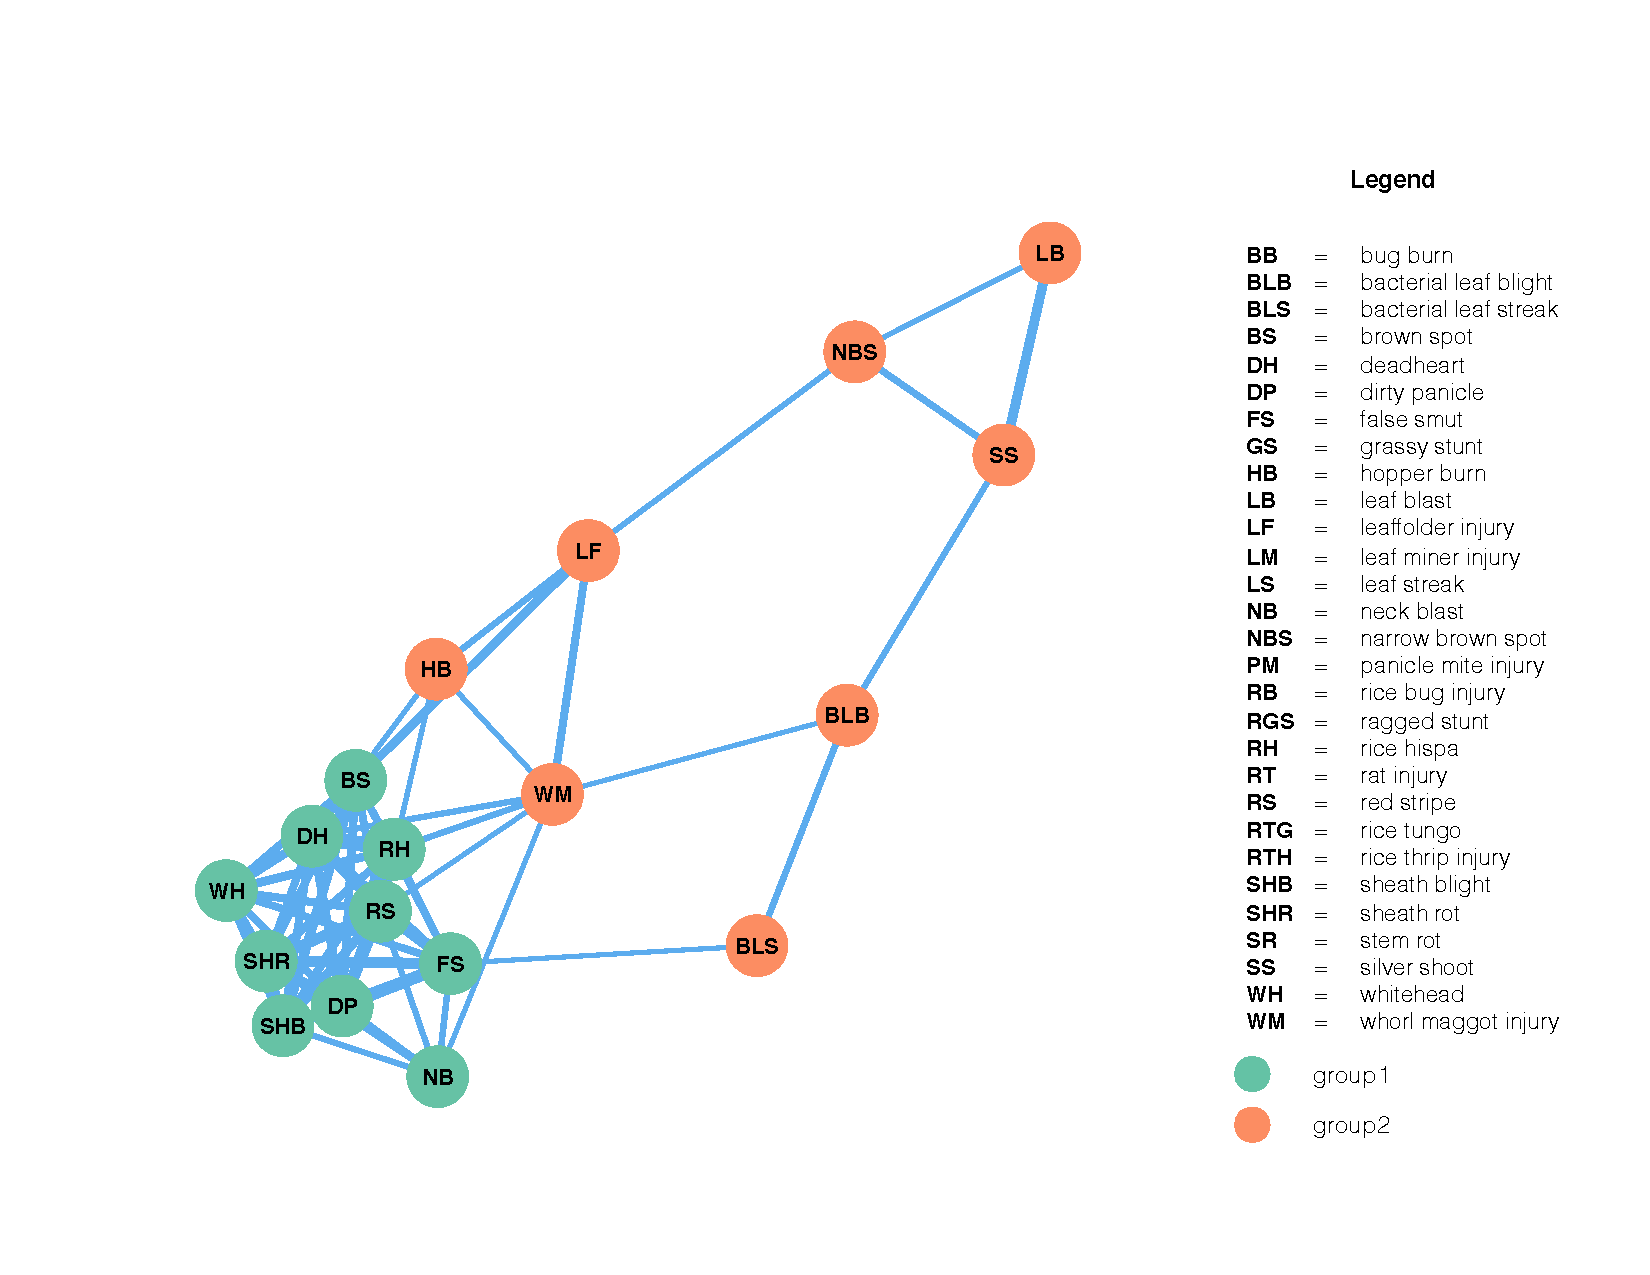
\includegraphics[width = 1\textwidth]{figures/networkCP_ds/networkCP_ds.pdf}
        \caption{Co-occurrence network of rice injuries in dry season at Central Plain, Thailand. The layout of the network graph is based on the Fruchterman-Reingold algorithm, which places nodes with stronger or more connections closer to each other.}
        \label{fig:networkCP_ds}
    \end{subfigure}
    \begin{subfigure}[b]{1\textwidth}
        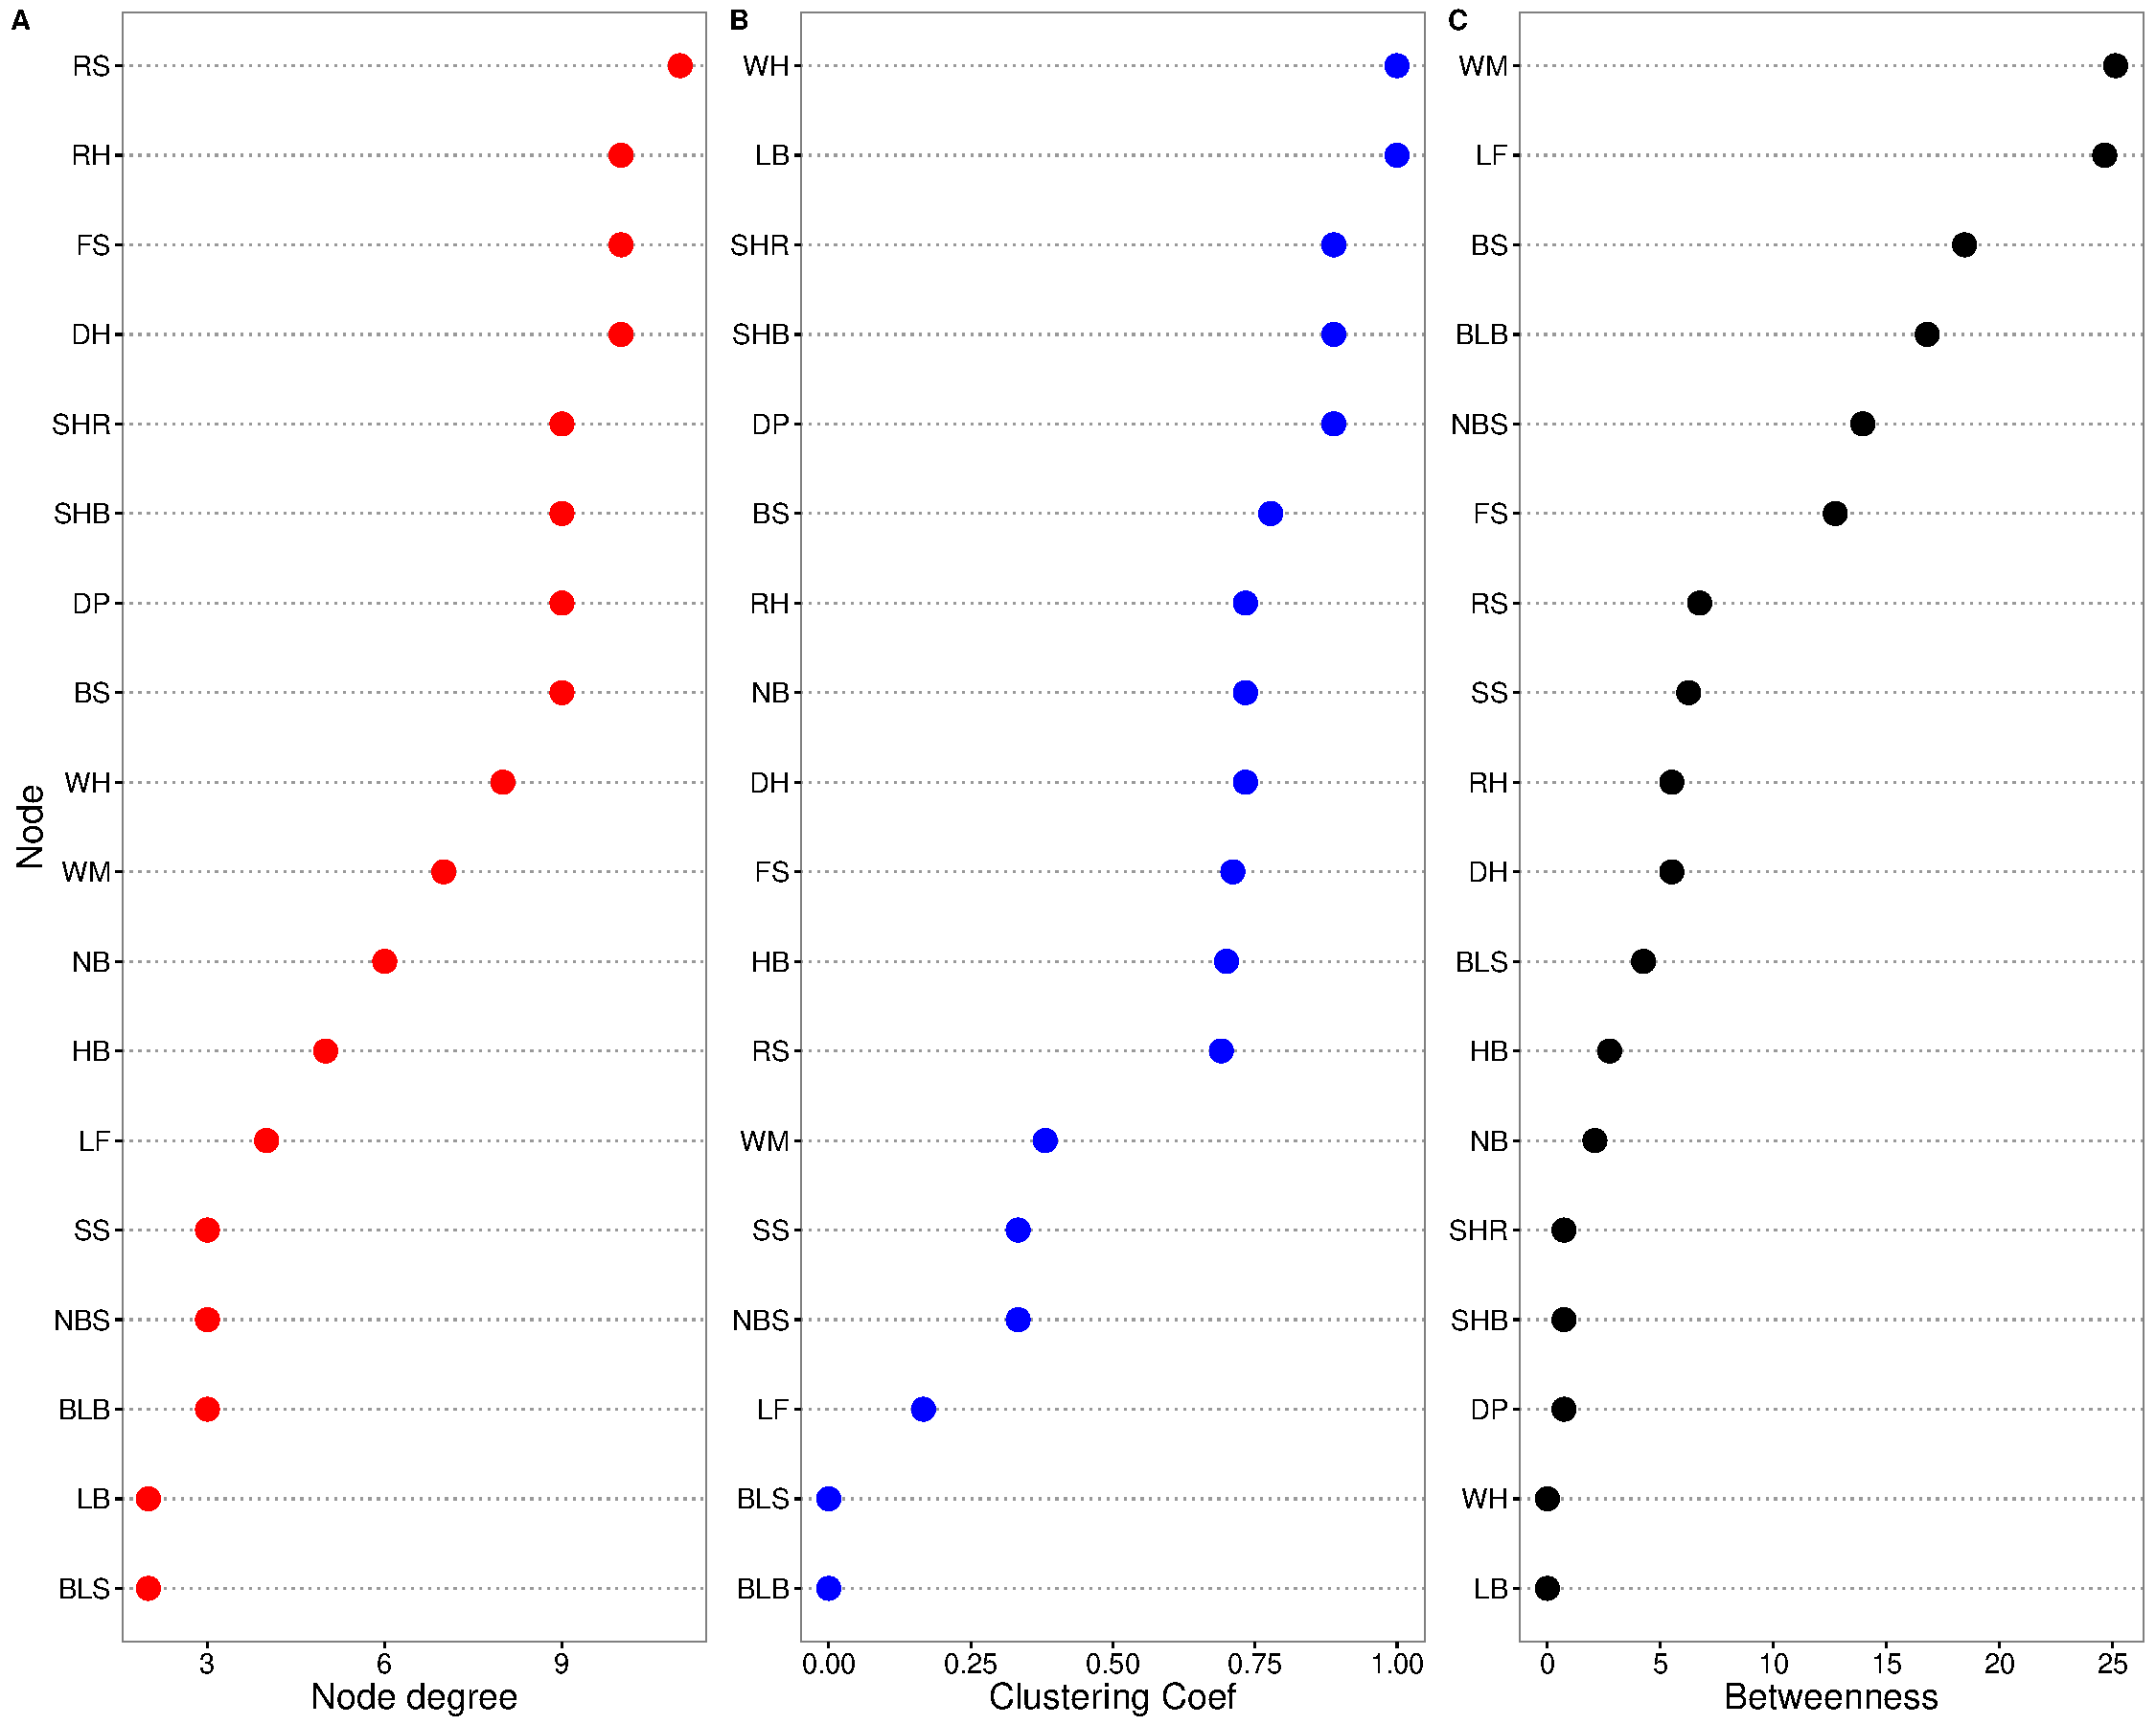
\includegraphics[width = 1\textwidth]{figures/nodepropCP_ds/nodepropCP_ds.pdf}
        \caption{Three centrality measures of the nodes in co-occurrence network of rice injuries in dry season at Central Plain. A: node degree, B:clustering coefficient, and C:Betweenness.}
        \label{fig:nodepropCP_ds}
    \end{subfigure}
    \caption{Rice injuries in dry season in Central Plain, Thailand}
    \label{fig:CP_ds}
\end{figure}

\begin{figure}
    \centering
    \begin{subfigure}[b]{1\textwidth}
        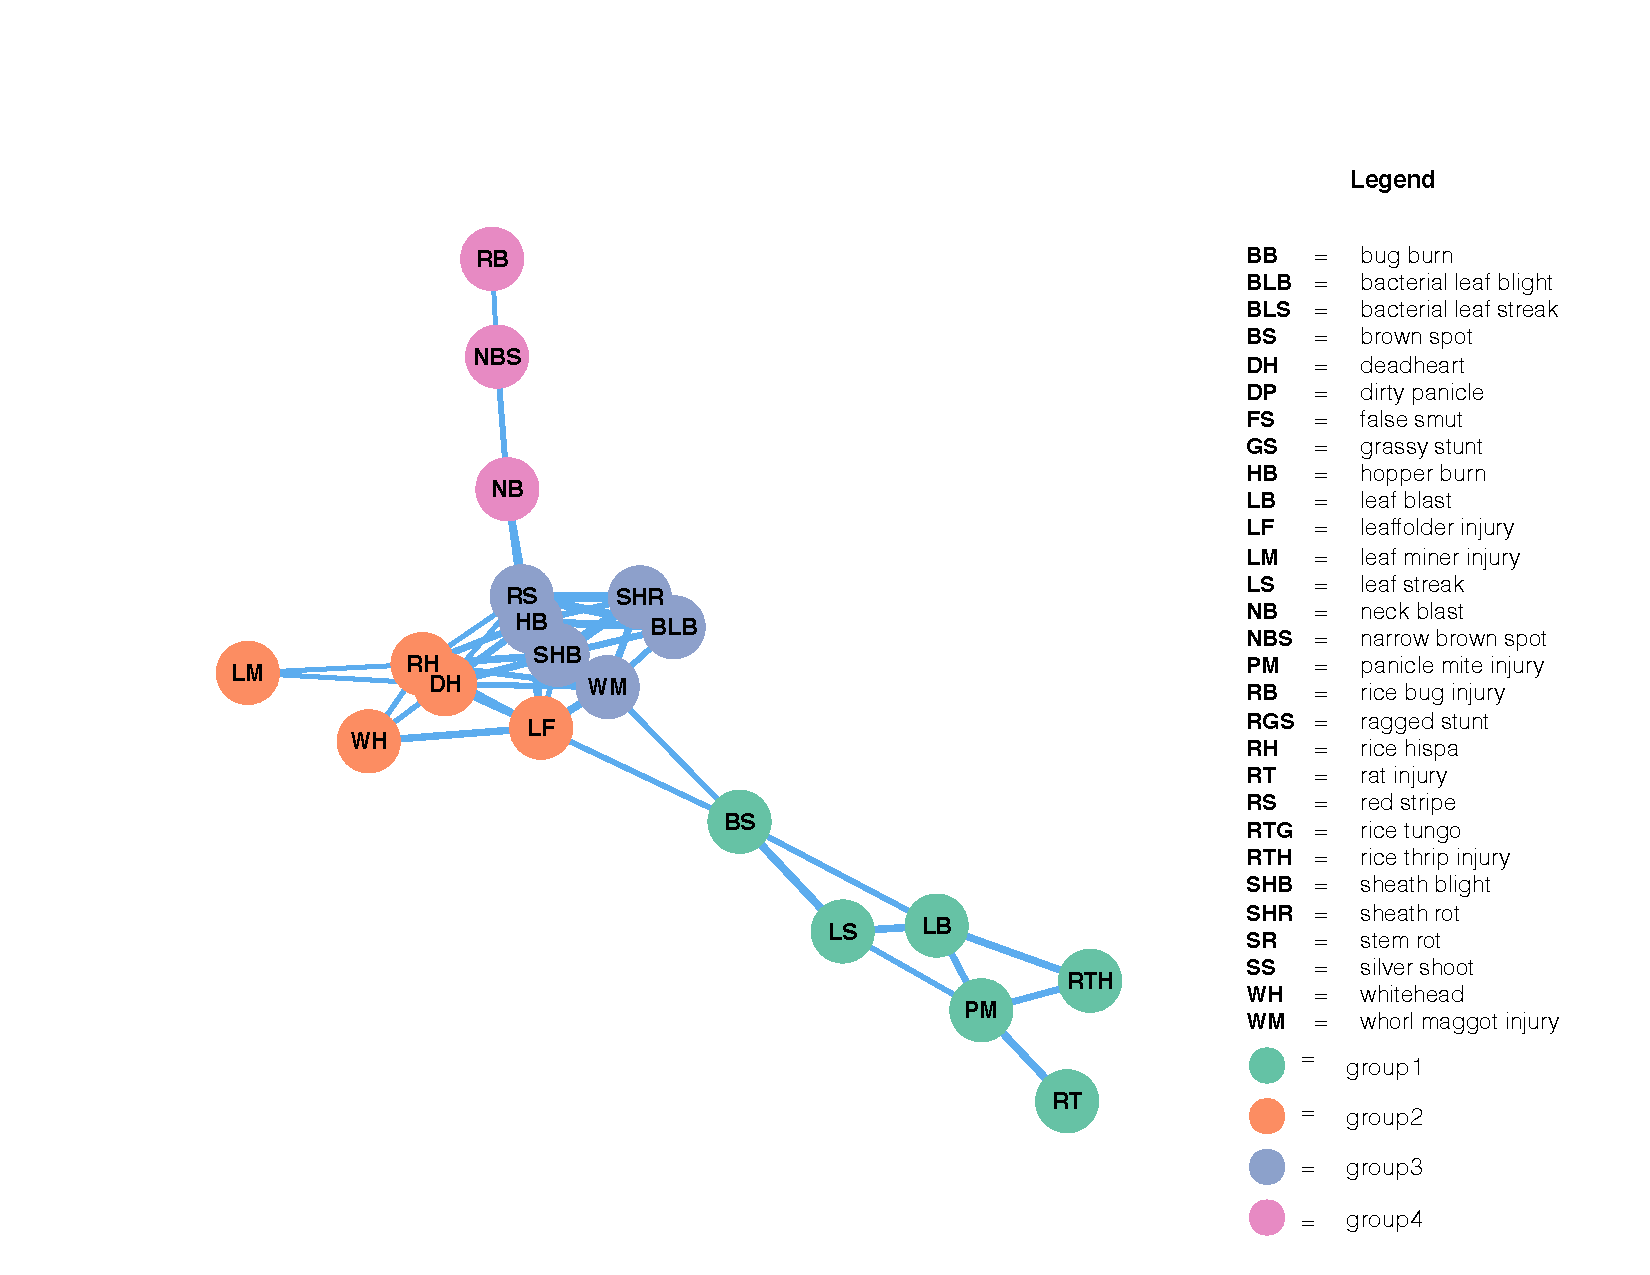
\includegraphics[width = 1\textwidth]{figures/networkCP_ws/networkCP_ws.pdf}
        \caption{Co-occurrence network of rice injuries in dry season at Central Plain, Thailand. The layout of the network graph is based on the Fruchterman-Reingold algorithm, which places nodes with stronger or more connections closer to each other.}
        \label{fig:networkCP_ws}
    \end{subfigure}
    \begin{subfigure}[b]{1\textwidth}
        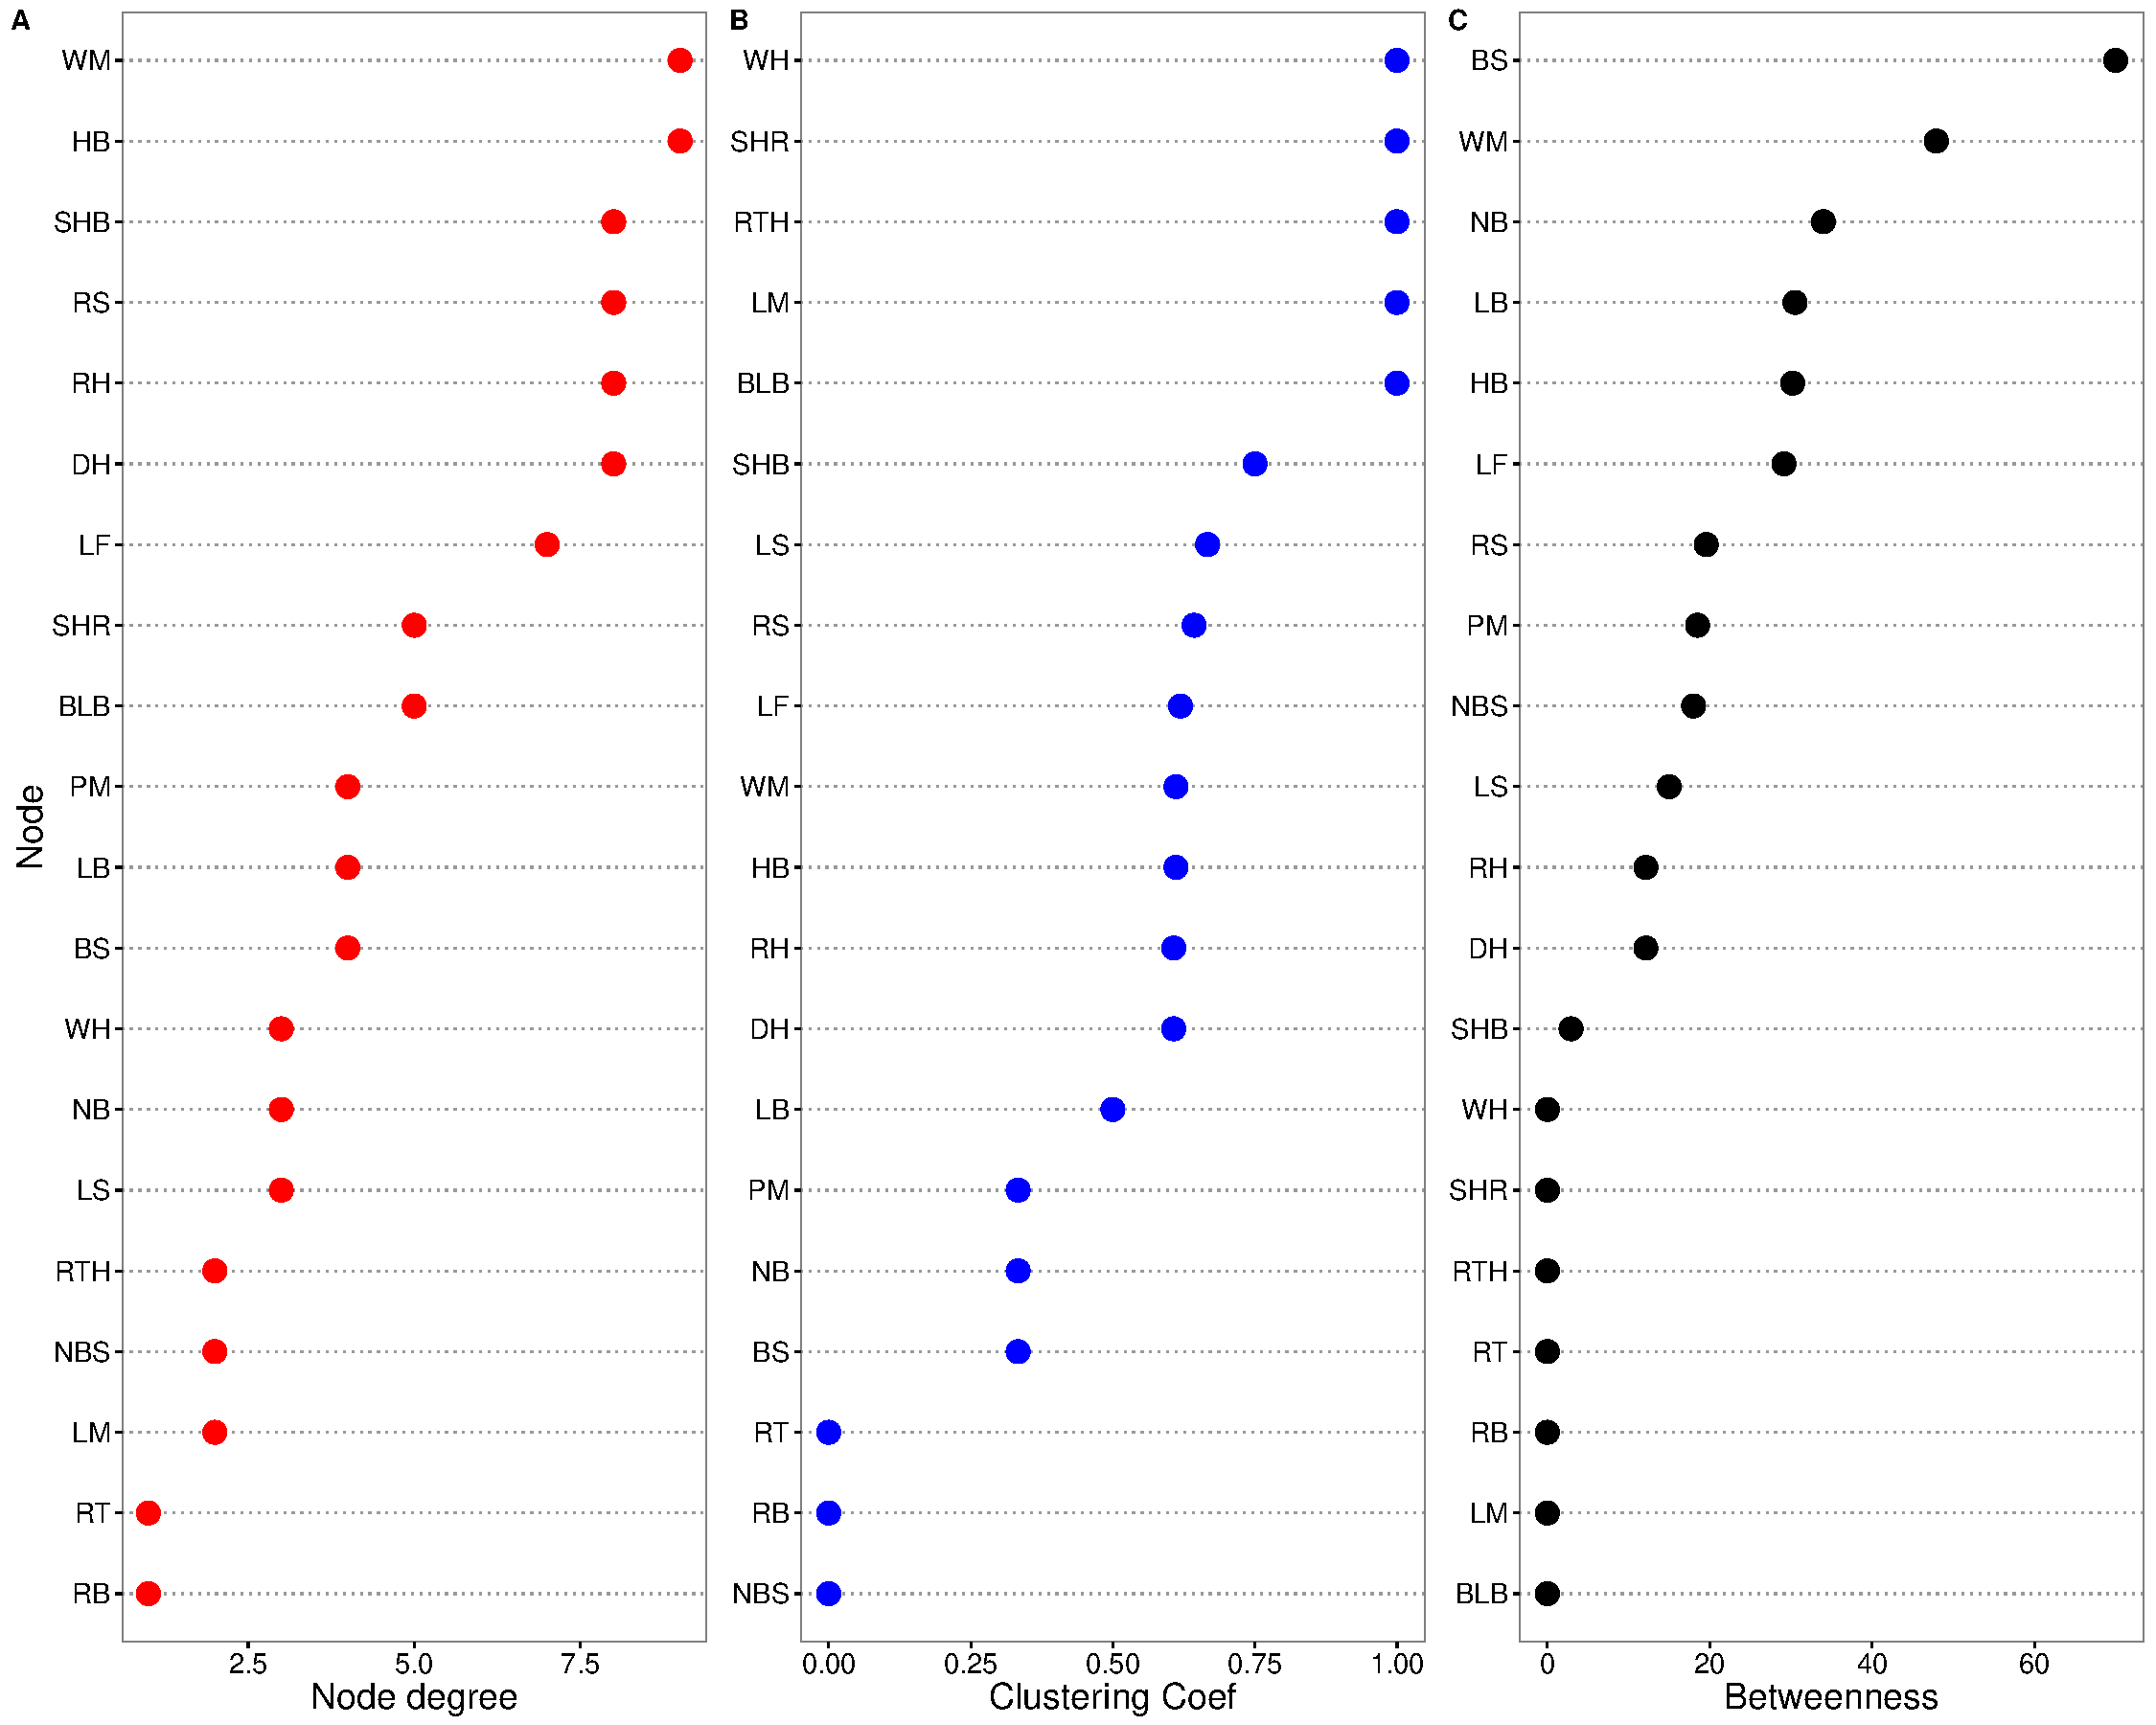
\includegraphics[width = 1\textwidth]{figures/nodepropCP_ws/nodepropCP_ws.pdf}
        \caption{Three centrality measures of the nodes in co-occurrence network of rice injuries in dry season at Central Plain. A: node degree, B:clustering coefficient, and C:Betweenness}
        \label{fig:nodepropCP_ds}
    \end{subfigure}
    \caption{Injuries in Central Plain, Thailand}
    \label{fig:CP_ws}
\end{figure}

\paragraph{Odisha, India}

Co-occurrence network of rice injuries in dry season (Figure \ref{fig:networkOR_ds}) was composed of ?? associated injuries and captured ?? associations. The network showed two isolated groups of injuries. Injuries within groups were closely related based on clustering coefficient (Table \ref{table:nodepropOR_ds}). This network could be inferred that there are two injury syndromes. One was the combination of BS, BLB, WM and SHB. Another was RH, WH, DH, LB, NB.

The network in wet season (Figure \ref{fig:networkOR_ws}) was more complex than dry season one. It composed of ?? nodes with ?? edges. The network reveals four groups of injury profiles. Group4 was isolated from the rest. Group2 was the biggest group placed in the middle of group1 and 3. The injuries in group2 had high node degree (table \ref{table:nodepropOR_ws}), which mean they were connected to many injuries. NBS and LF, injuries in group1 and group2, respectively presented high betweenness values and connected to injuries of group3. This indicated that group3 injuries had high chance to occur together with group1 and 2, but not group4. 

\begin{figure}
    \centering
    \begin{subfigure}[b]{1\textwidth}
        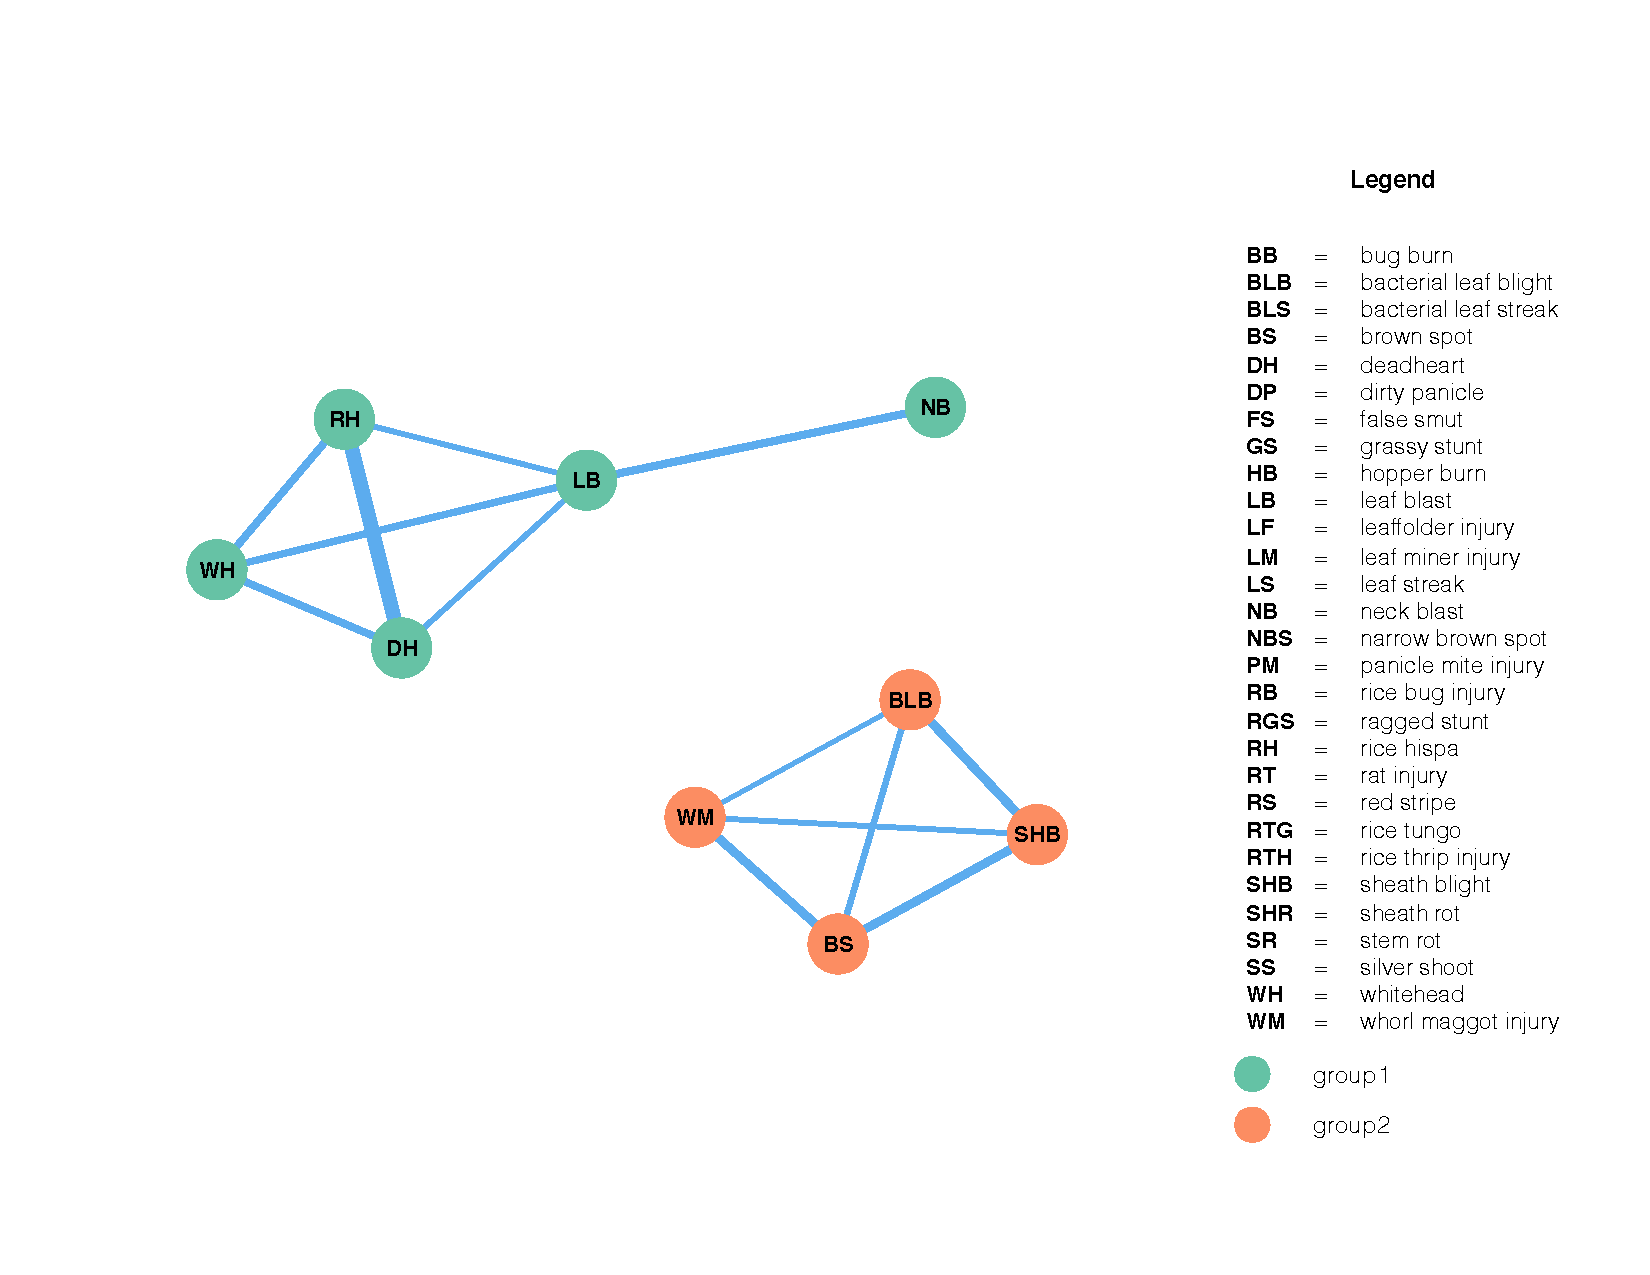
\includegraphics[width = 1\textwidth]{figures/networkOR_ds/networkOR_ds.pdf}
        \caption{Co-occurrence network of rice injuries in wet season at Odisha, India. The layout of the network graph is based on the Fruchterman-Reingold algorithm, which places nodes with stronger or more connections closer to each other.}
        \label{fig:networkOR_ds}
    \end{subfigure}
    \begin{subfigure}[b]{1\textwidth}
        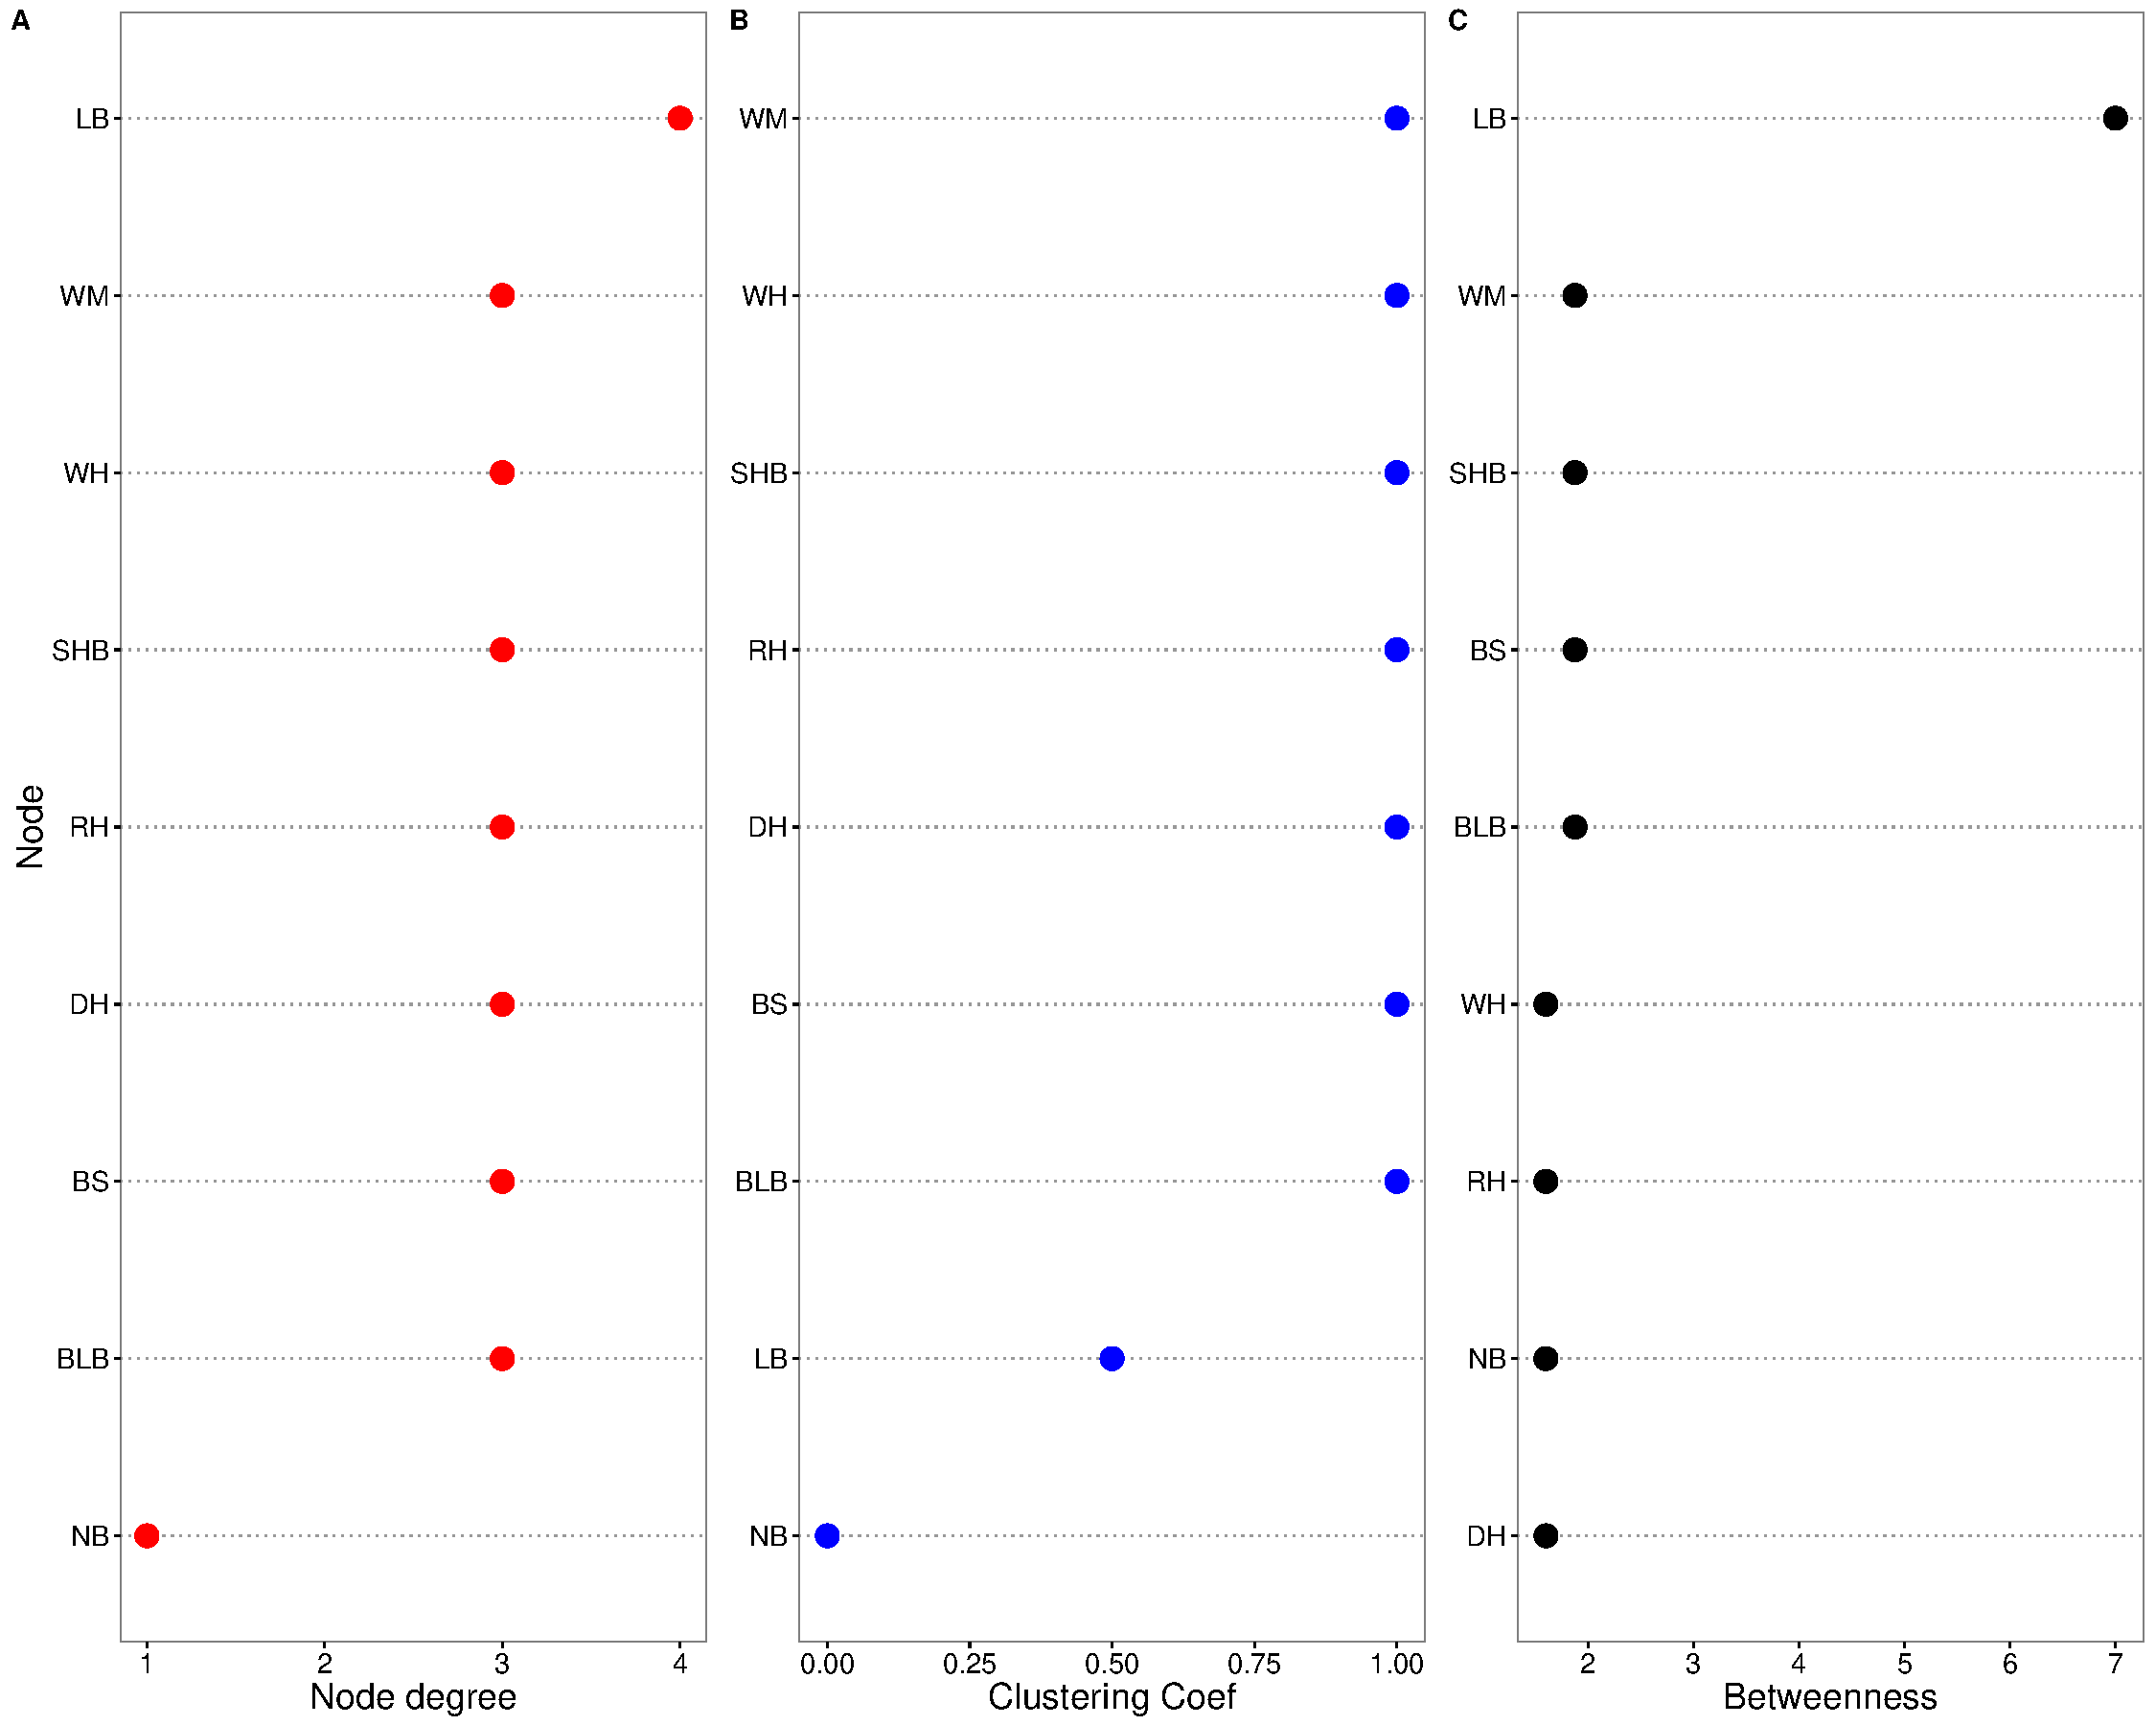
\includegraphics[width = 1\textwidth]{figures/nodepropOR_ds/nodepropOR_ds.pdf}
        \caption{Three centrality measures of the nodes in co-occurrence network of rice injuries in dry season at Odisha, India. A: node degree, B:clustering coefficient, and C:Betweenness, and.}
        \label{fig:nodepropCP_ds}
    \end{subfigure}
    \caption{Injuries in dry season at Odisha, India}
    \label{fig:OR_ds}
\end{figure}

\begin{figure}
    \centering
    \begin{subfigure}[b]{1\textwidth}
        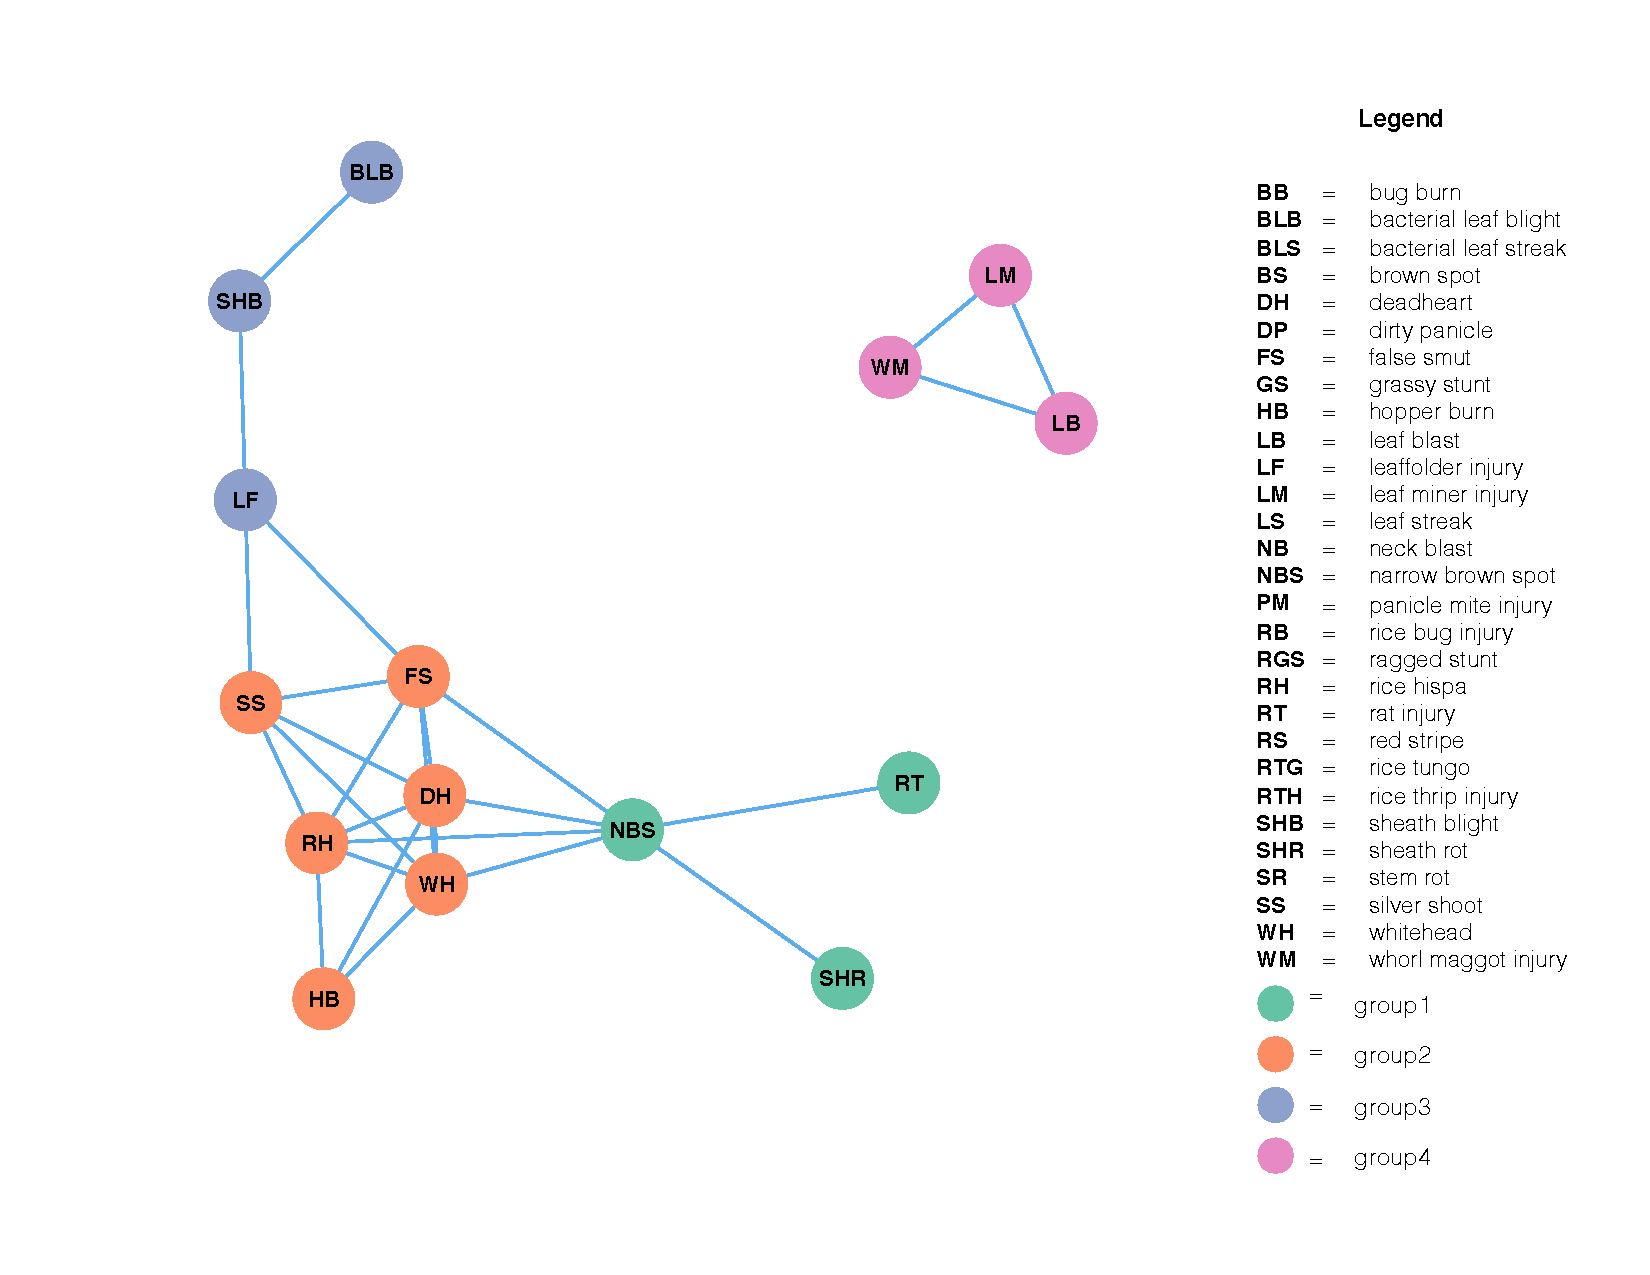
\includegraphics[width = 1\textwidth]{figures/networkOR_ws/networkOR_ws.pdf}
        \caption{Co-occurrence network of rice injuries in wet season at Odisha, India. The layout of the network graph is based on the Fruchterman-Reingold algorithm, which places nodes with stronger or more connections closer to each other.}
        \label{fig:gull}
    \end{subfigure}
    \begin{subfigure}[b]{1\textwidth}
        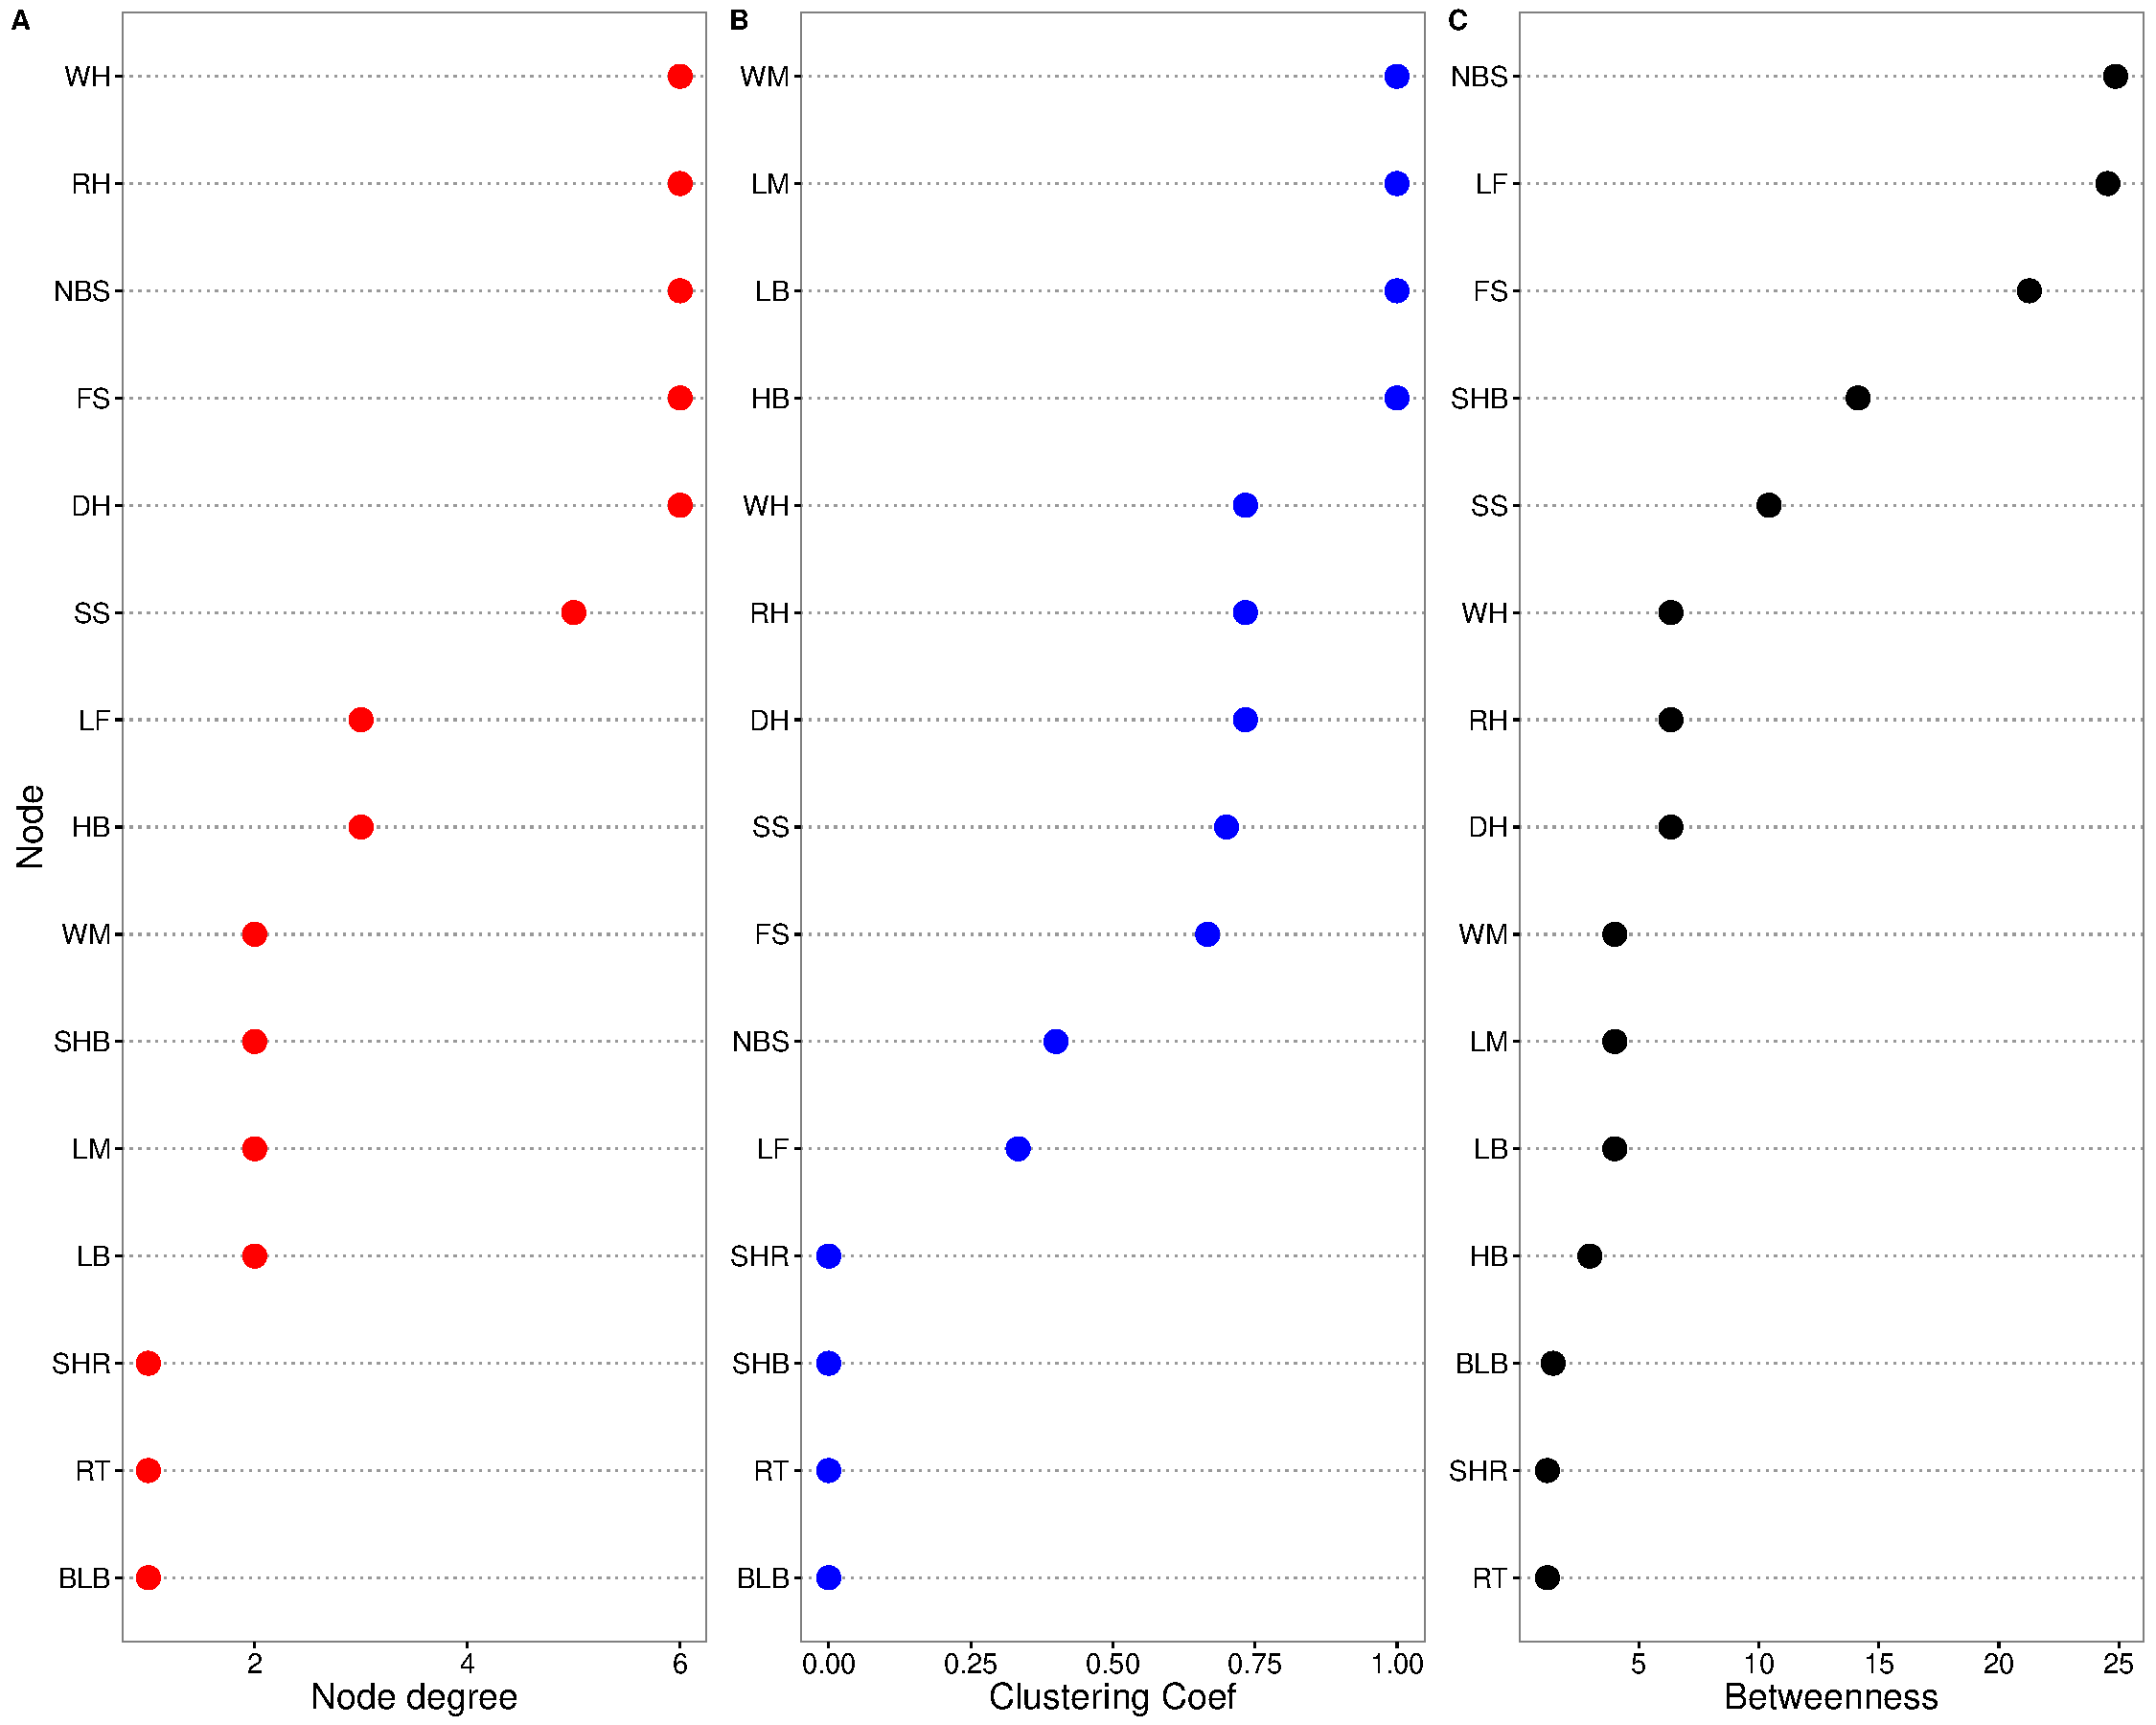
\includegraphics[width = 1\textwidth]{figures/nodepropOR_ws/nodepropOR_ws.pdf}
        \caption{Three centrality measures of the nodes in co-occurrence network of rice injuries in wet season at Odisha, India. A: node degree, B:clustering coefficient, and C:Betweenness, and.}
        \label{fig:nodepropCP_ds}
    \end{subfigure}
    \caption{Injuries in wer season at Odisha, India}
    \label{fig:OD_ws}
\end{figure}


\paragraph{Red River Delta, Vietnam}
 
Co-occurrence network of rice injuries in dry season (Fig. \ref{fig:networkRR_ds}) composed of ?? nodes and ?? associations. The network reveals three isolated groups, and two connected groups of injury profiles. Group1 and group3 were linked with BB. Group3 was the biggest among the others. In this group, SHB, BS were nodes showing high centrality (table \ref{table:nodepropRR_ds}). If they were observed in rice fields, there was high chance to observe other injuries of group3 in the fields too.

Wet season network (Fig. \ref{fig:networkRR_ws})) composed of ?? injuries with ?? associations. It reveals 4 connected groups and one isolated small group of injury profiles. Group4 was located that could connect to Group2, 3, 5. According to table\ref{table:nodepropRR_ws}, BLB, DP could be a good indicator, because it was likely to occur (high betweenness) and when it presented, other injuries in other group, except group5 (high node degree). 


\begin{figure}
    \centering
    \begin{subfigure}[b]{1\textwidth}
        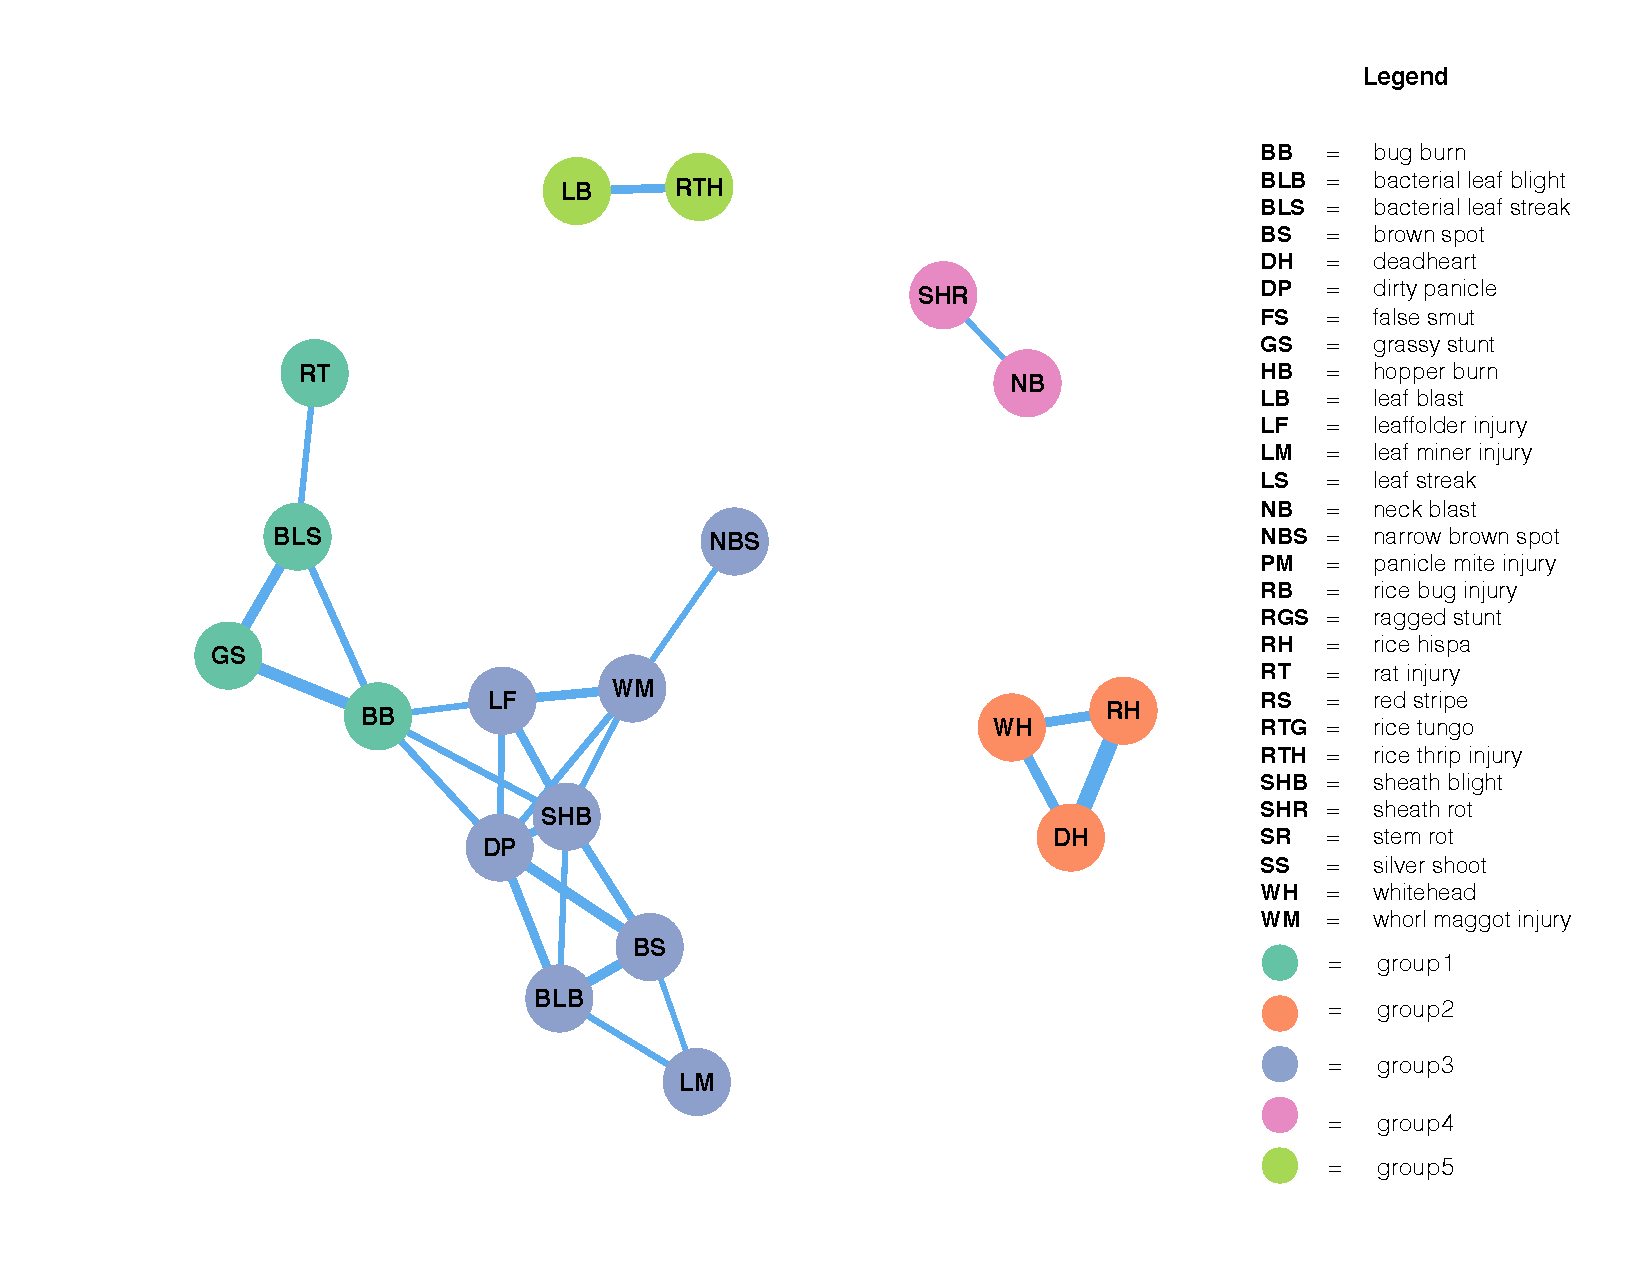
\includegraphics[width = 1\textwidth]{figures/networkRR_ds/networkRR_ds.pdf}
        \caption{Co-occurrence network of rice injuries in dry season at Red River Delta, Vietnam. The layout of the network graph is based on the Fruchterman-Reingold algorithm, which places nodes with stronger or more connections closer to each other.}
        \label{fig:gull}
    \end{subfigure}
    \begin{subfigure}[b]{1\textwidth}
        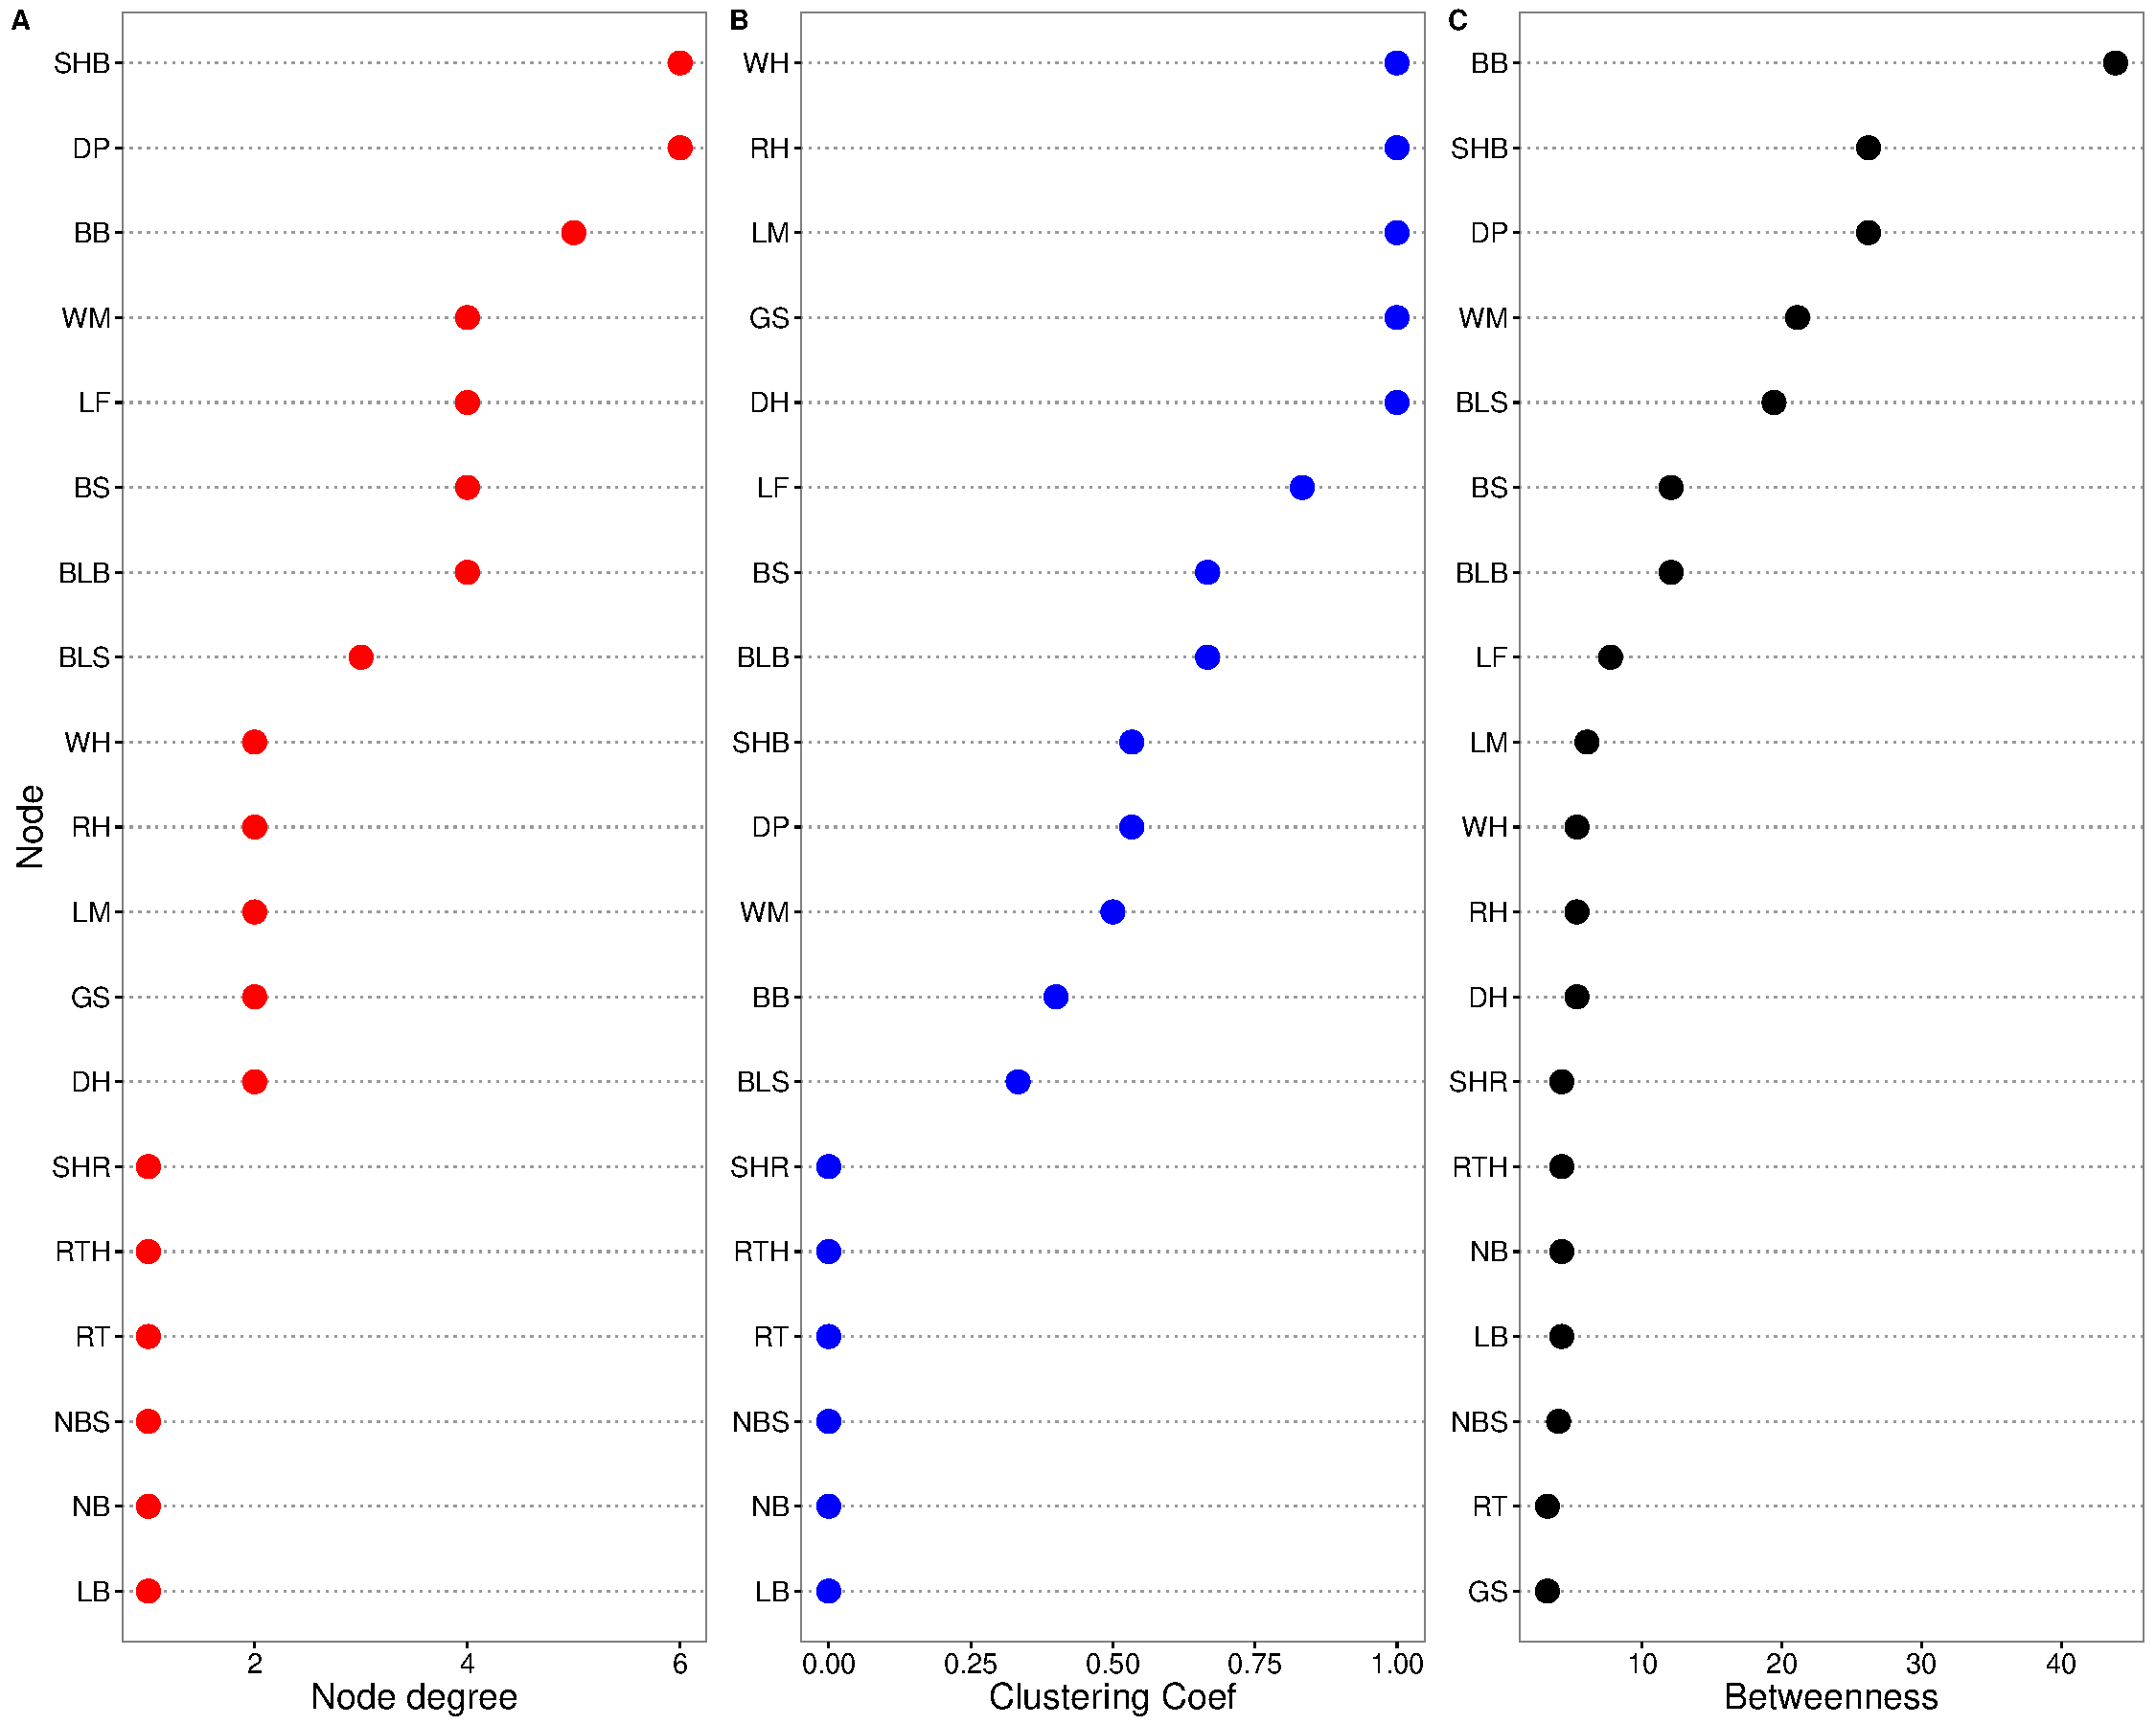
\includegraphics[width = 1\textwidth]{figures/nodepropRR_ds/nodepropRR_ds.pdf}
        \caption{Three centrality measures of the nodes in co-occurrence network of rice injuries in dry season at Red River Delta, Vietnam. A: node degree, B:clustering coefficient, and C:Betweenness}
        \label{fig:nodepropCP_ds}
    \end{subfigure}
    \caption{Pictures of animals}
    \label{fig:animals}
\end{figure}

\begin{figure}
    \centering
    \begin{subfigure}[b]{1\textwidth}
        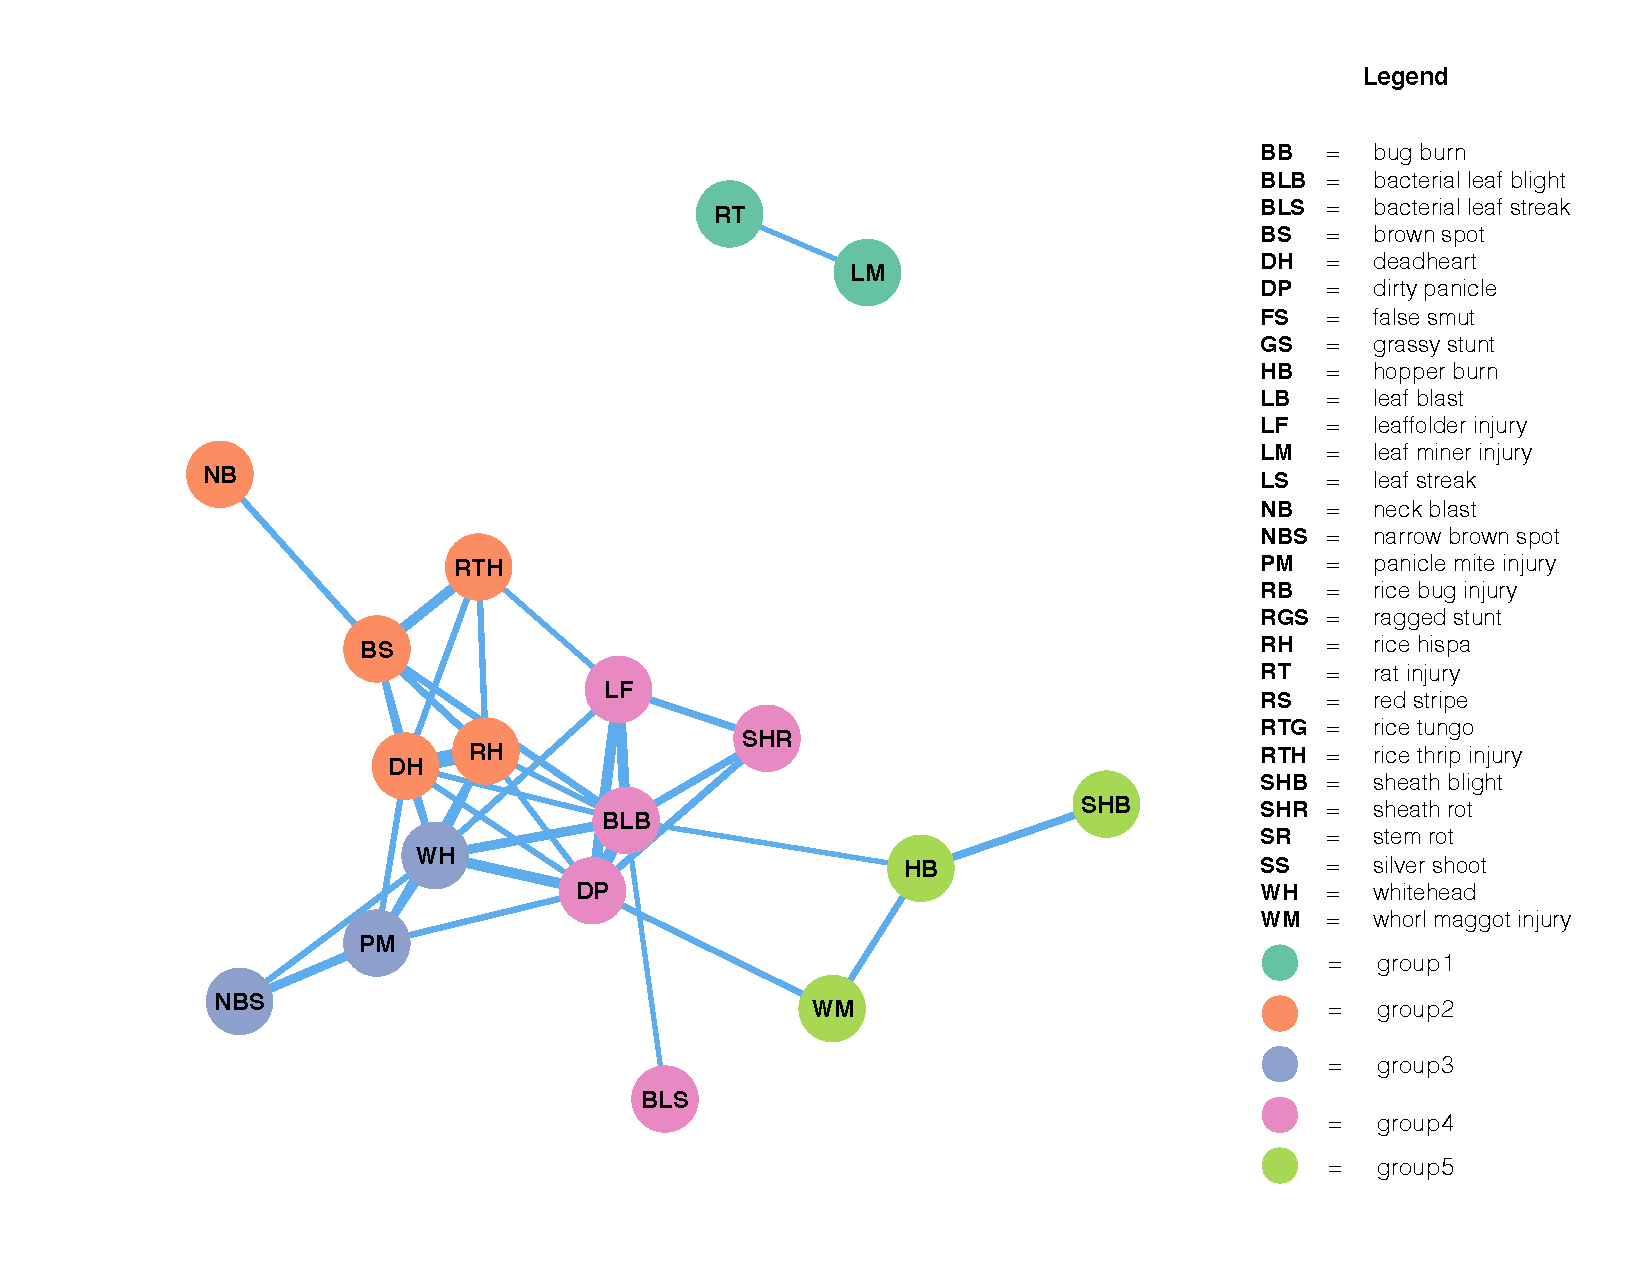
\includegraphics[width = 1\textwidth]{figures/networkRR_ws/networkRR_ws.pdf}
        \caption{Co-occurrence network of rice injuries in wet season at Red River Delta, Vietnam. The layout of the network graph is based on the Fruchterman-Reingold algorithm, which places nodes with stronger or more connections closer to each other.}
        \label{fig:gull}
    \end{subfigure}
    \begin{subfigure}[b]{1\textwidth}
        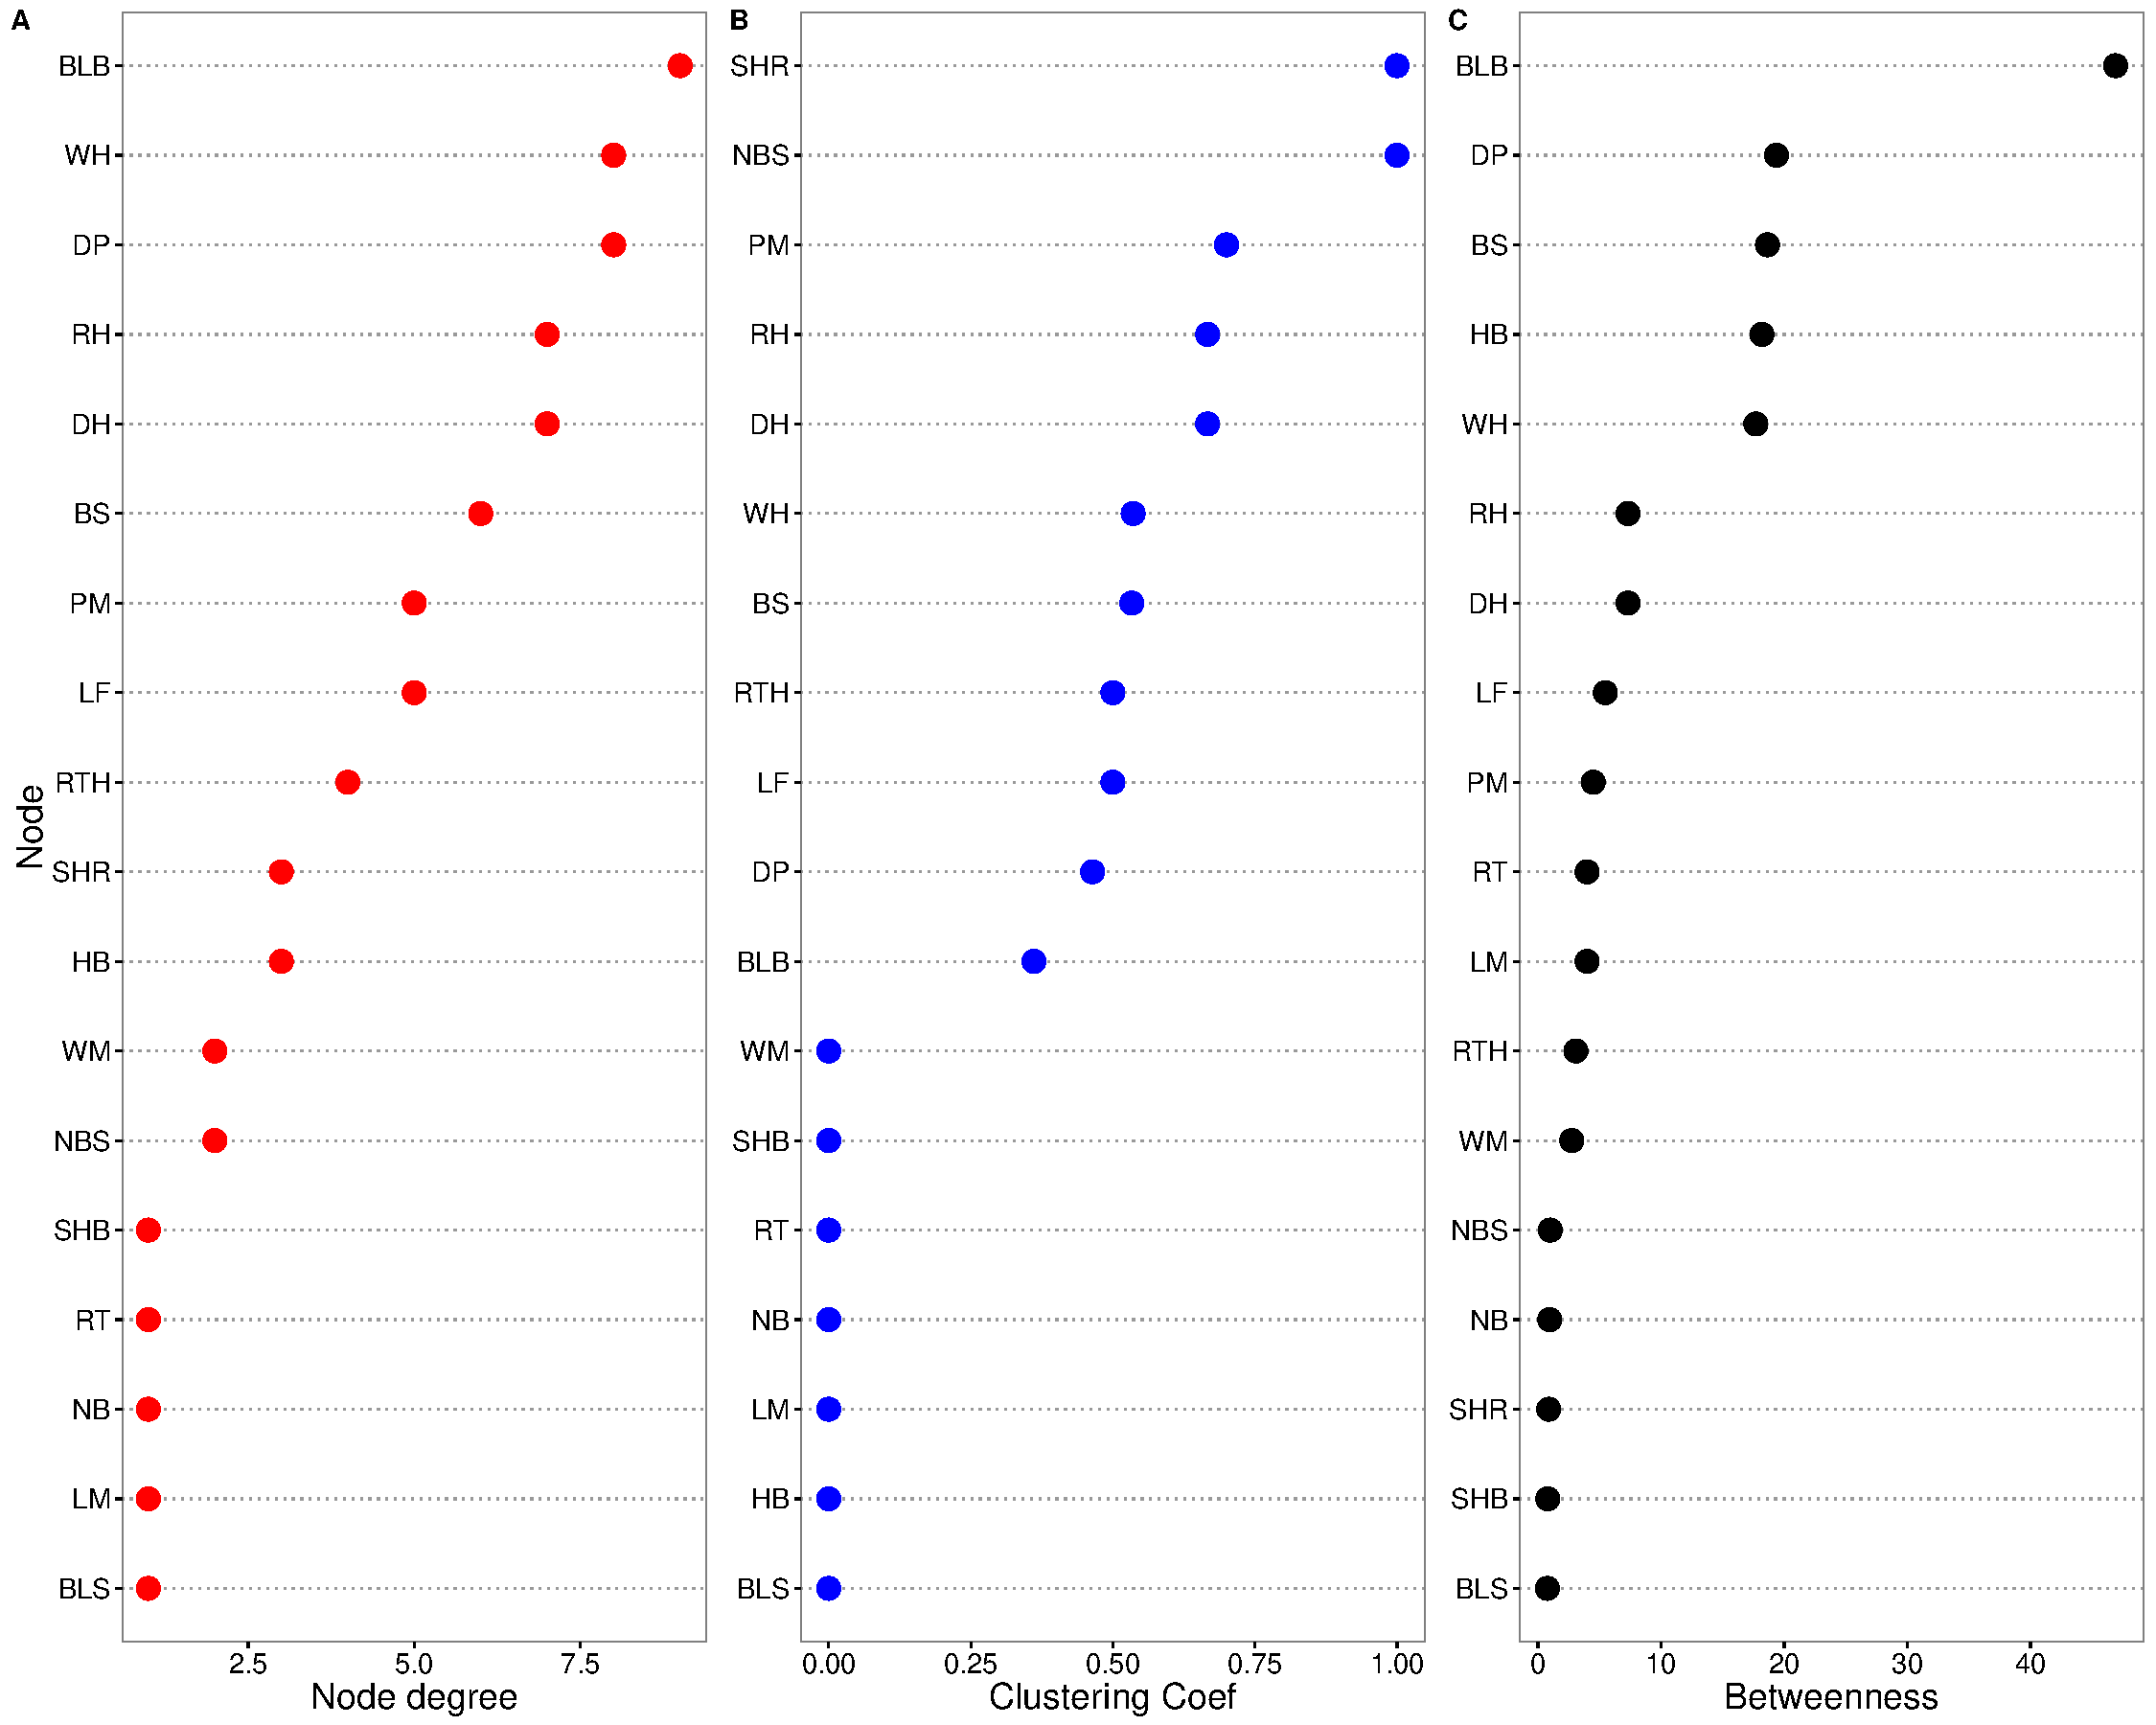
\includegraphics[width = 1\textwidth]{figures/nodepropRR_ws/nodepropRR_ws.pdf}
        \caption{Three centrality measures of the nodes in co-occurrence network of rice injuries in wet season at Red River Delta, Vietnam. A: node degree, B:clustering coefficient, and C:Betweenness}
        \label{fig:nodepropCP_ds}
    \end{subfigure}
    \caption{Rice injuries in wet season in Red River Delta, Vietnam}
    \label{fig:animals}
\end{figure}


\paragraph{Tamil Nadu, India}

The dry season network (Fig \ref{fig:networkTM_ds}) revealed three clustered groups of injury profiles. One of them was separated from other two. Group1 was condensed, which differ from group2 that injuries were placed further. SHB and BLB were disconnected to the rest.  BS and WH highly tended to occur in this season (high betweenness).  Because clustering coefficient value of members in group2 less than group1, injuries in group2 might occur together with one or two more injuries. But in group1, the combination was more complex than.

Figure \ref{fig:networkTM_ws} presented co-occurrence network of injury profiles in dry season. Network resulted three groups of injury profiles. Compared to other groups, group3 had less connection. Group1 had high node degree injuires.


\begin{figure}
    \centering
    \begin{subfigure}[b]{1\textwidth}
        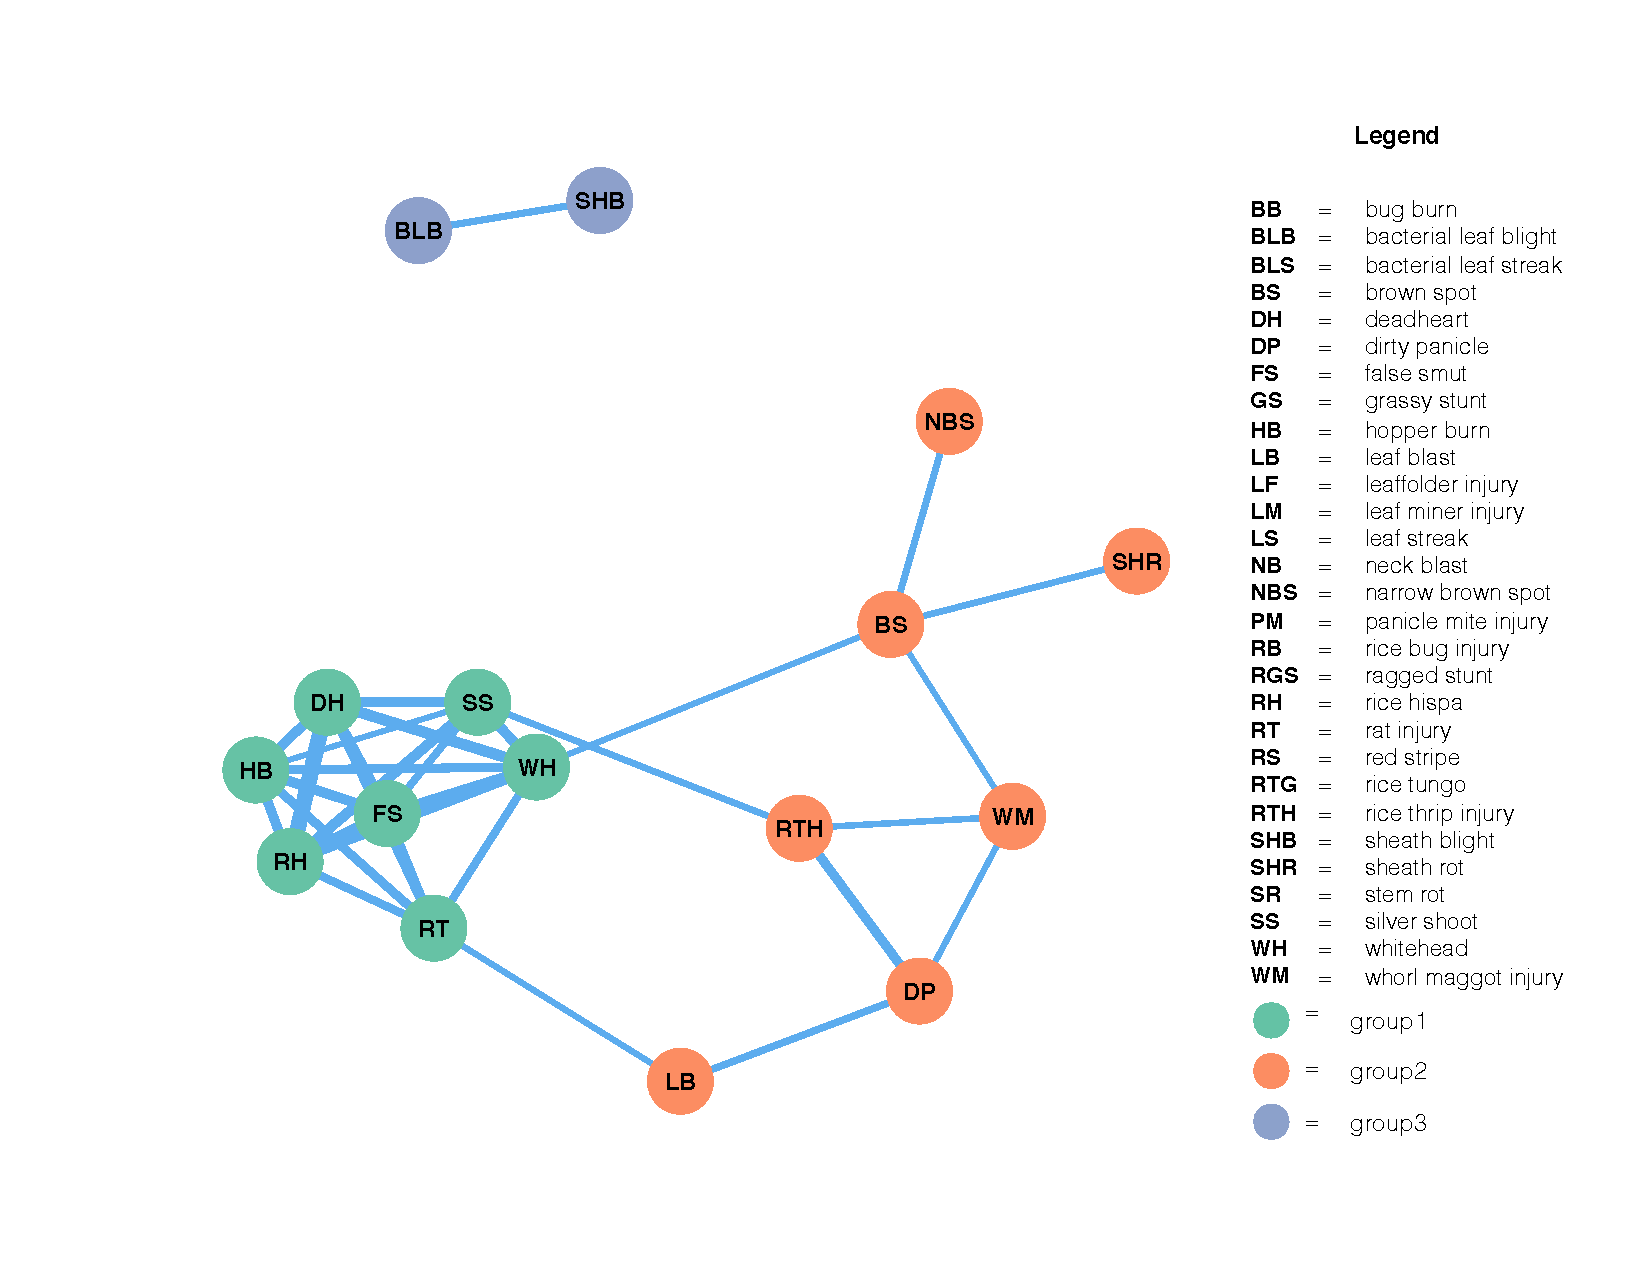
\includegraphics[width = 1\textwidth]{figures/networkTM_ds/networkTM_ds.pdf}
        \caption{Co-occurrence network of rice injuries in dry season at Tamil Nadu, India. The layout of the network graph is based on the Fruchterman-Reingold algorithm, which places nodes with stronger or more connections closer to each other.}
        \label{fig:networkTM_ds}
    \end{subfigure}
    \begin{subfigure}[b]{1\textwidth}
        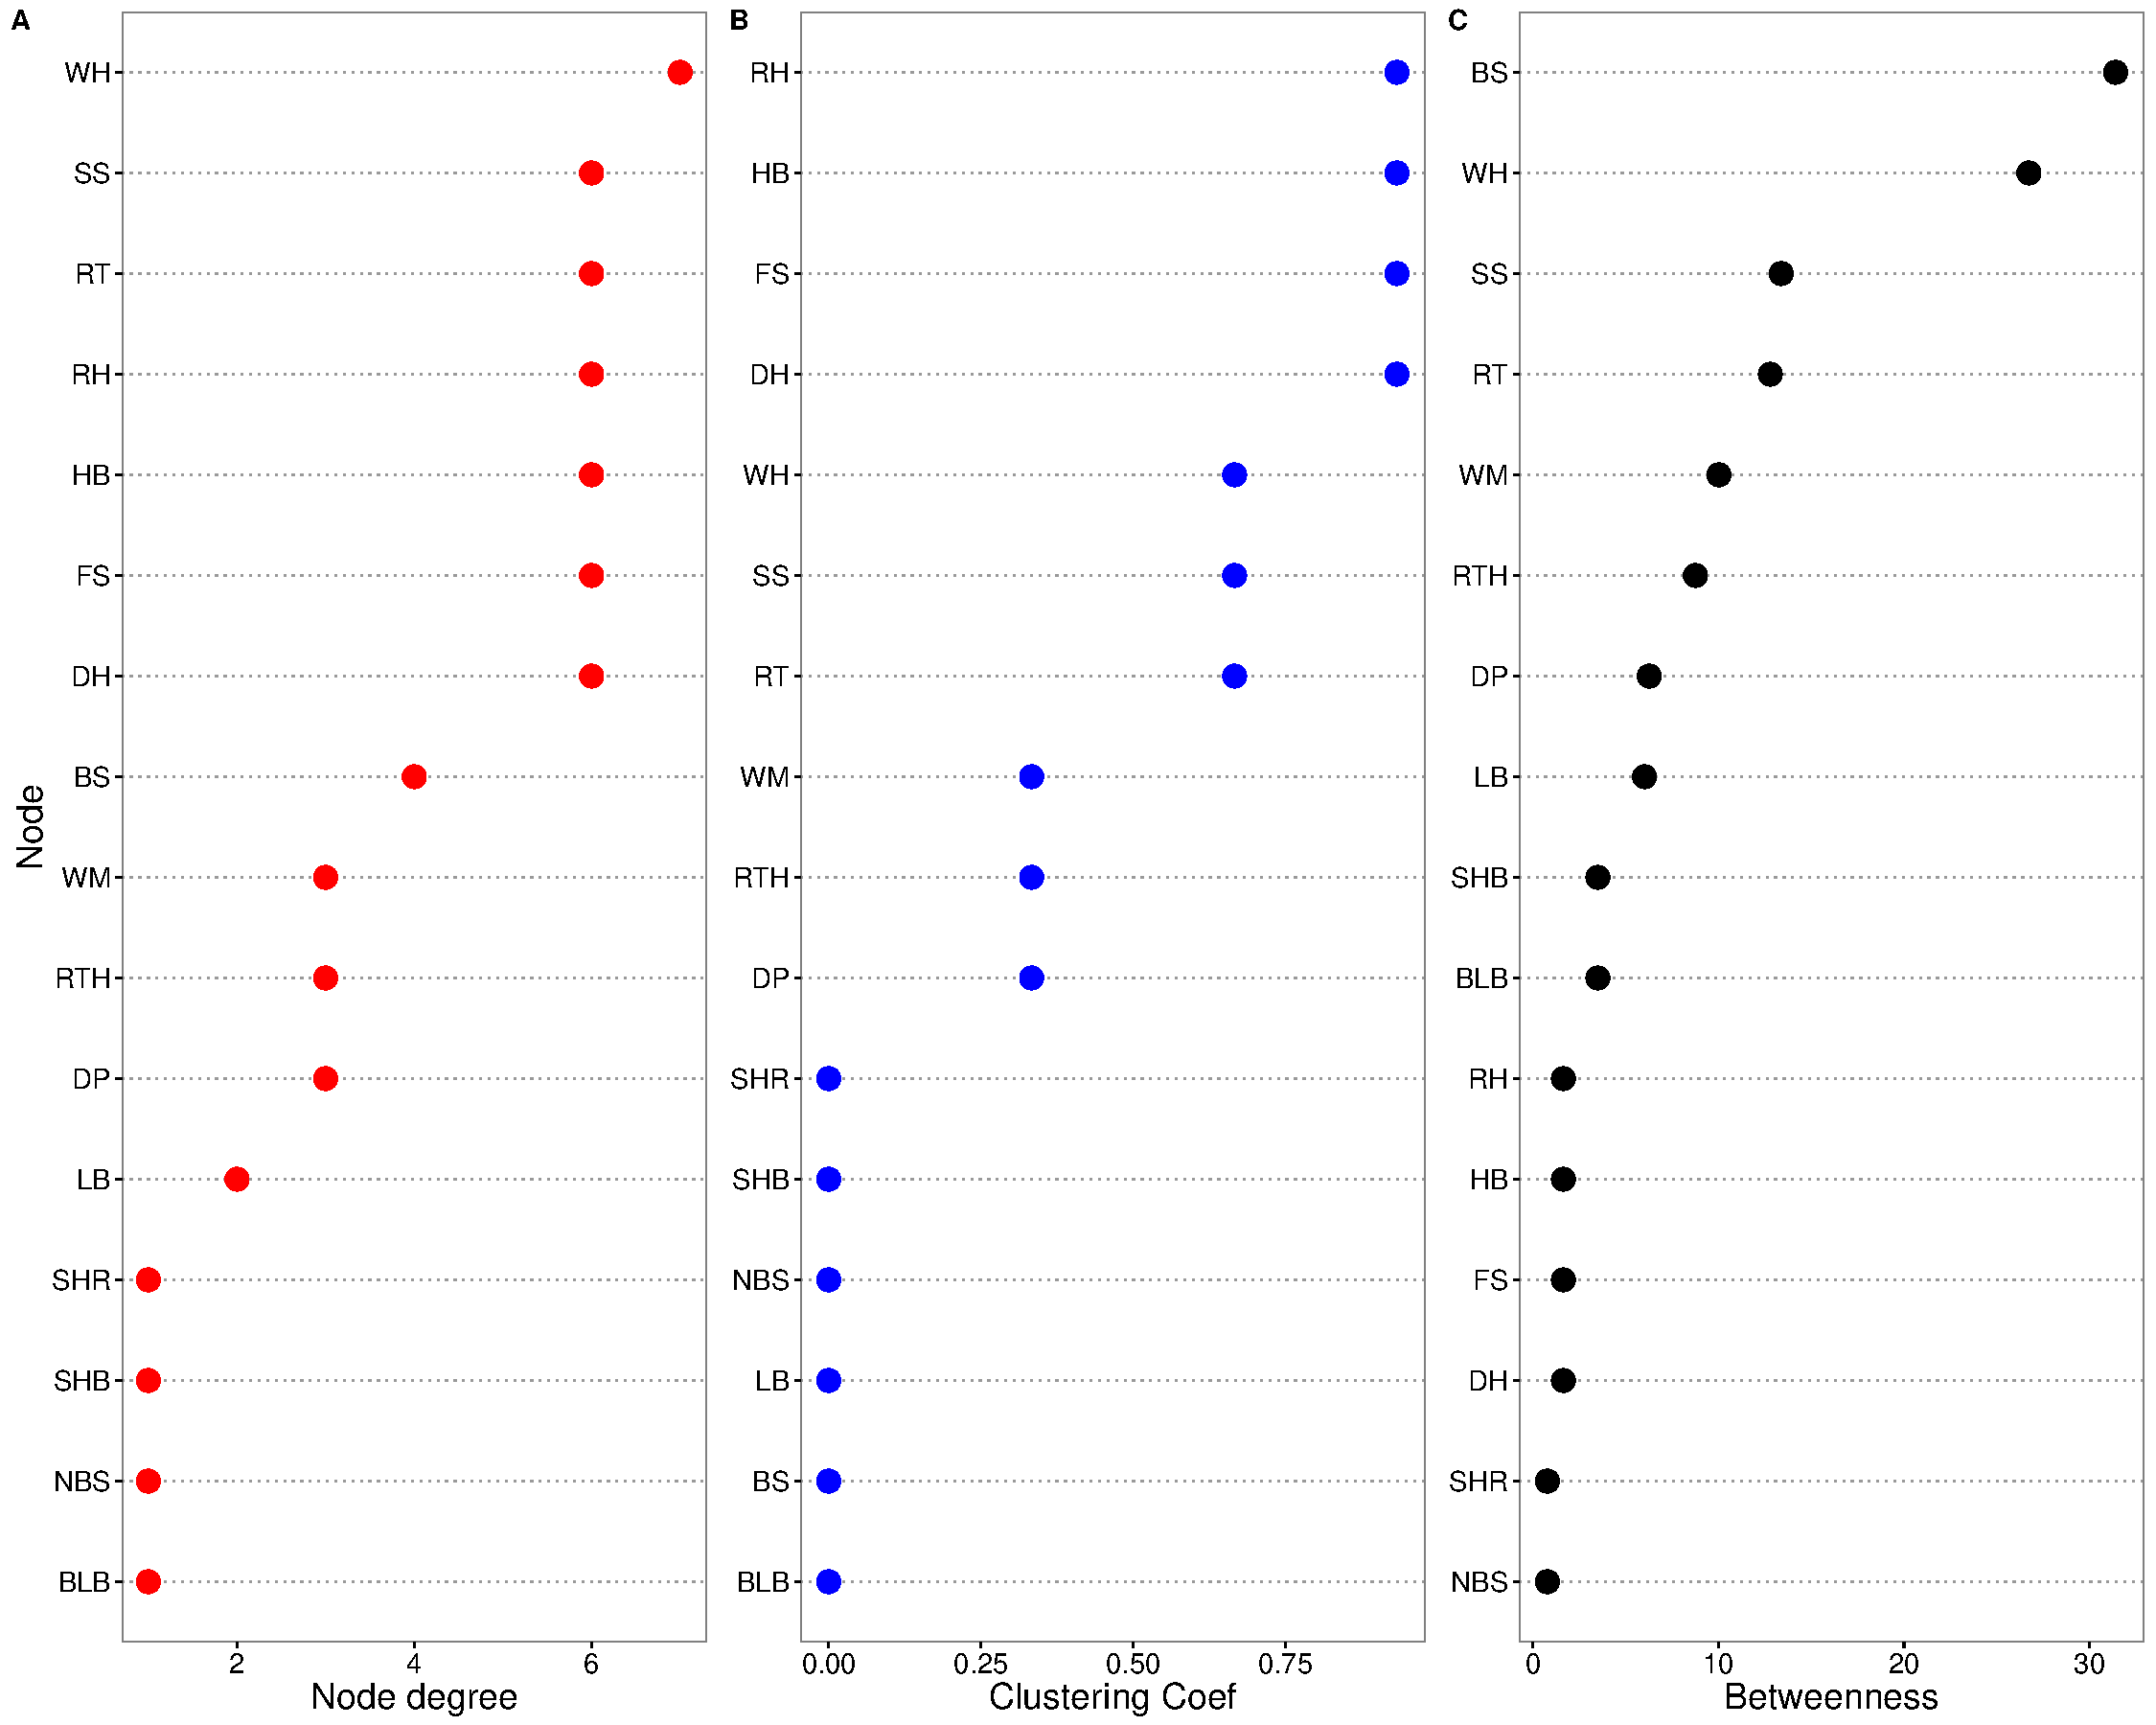
\includegraphics[width = 1\textwidth]{figures/nodepropTM_ds/nodepropTM_ds.pdf}
        \caption{Three centrality measures of the nodes in co-occurrence network of rice injuries in dry season at Tamil Nadu, India. A: node degree, B:clustering coefficient, and C:Betweenness, and.}
        \label{fig:nodepropTM_ds}
    \end{subfigure}
    \caption{Rice injuries in dry season in Tamil Nadu, India}
    \label{fig:TM_ds}
\end{figure}

\begin{figure}
    \centering
    \begin{subfigure}[b]{1\textwidth}
        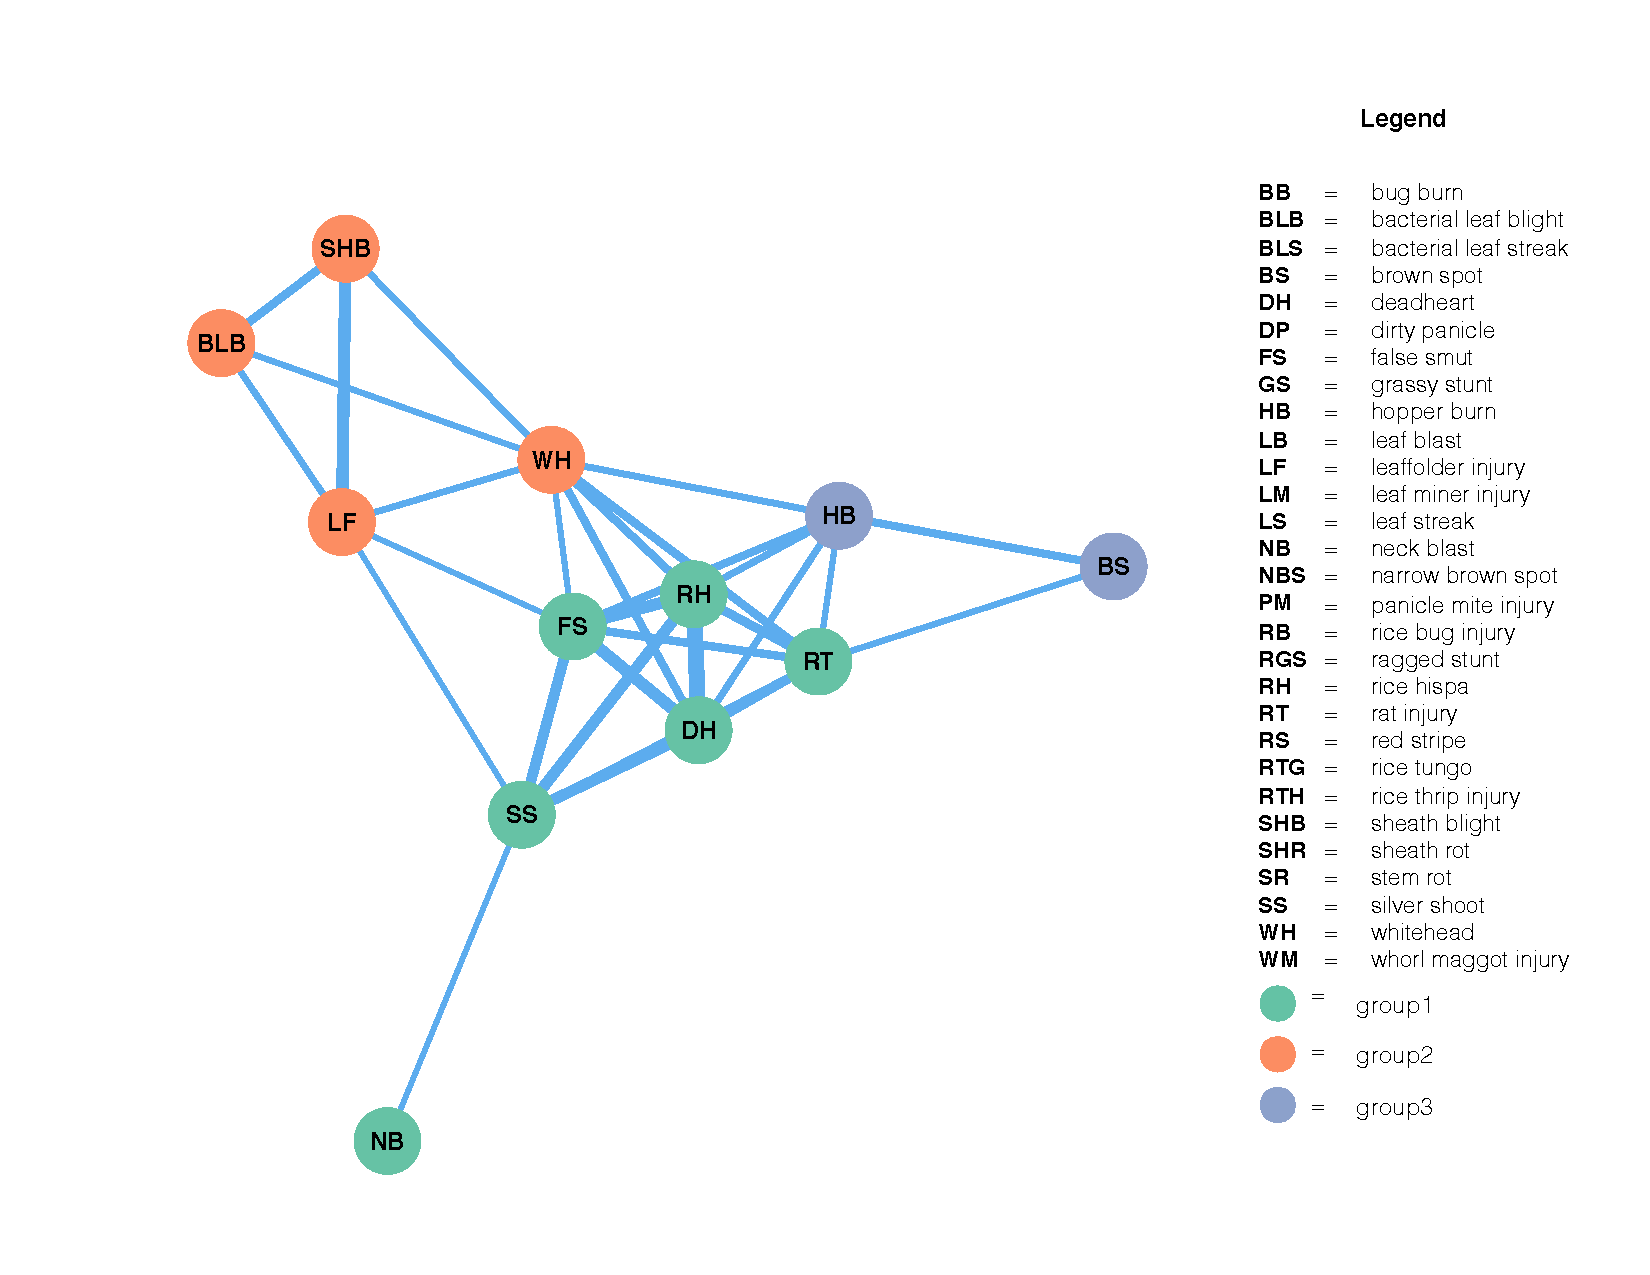
\includegraphics[width = 1\textwidth]{figures/networkTM_ws/networkTM_ws.pdf}
        \caption{Co-occurrence network of rice injuries in wet season at Tamil Nadu, India. The layout of the network graph is based on the Fruchterman-Reingold algorithm, which places nodes with stronger or more connections closer to each other.}
        \label{fig:networkTM_ws}
    \end{subfigure}
    \begin{subfigure}[b]{1\textwidth}
        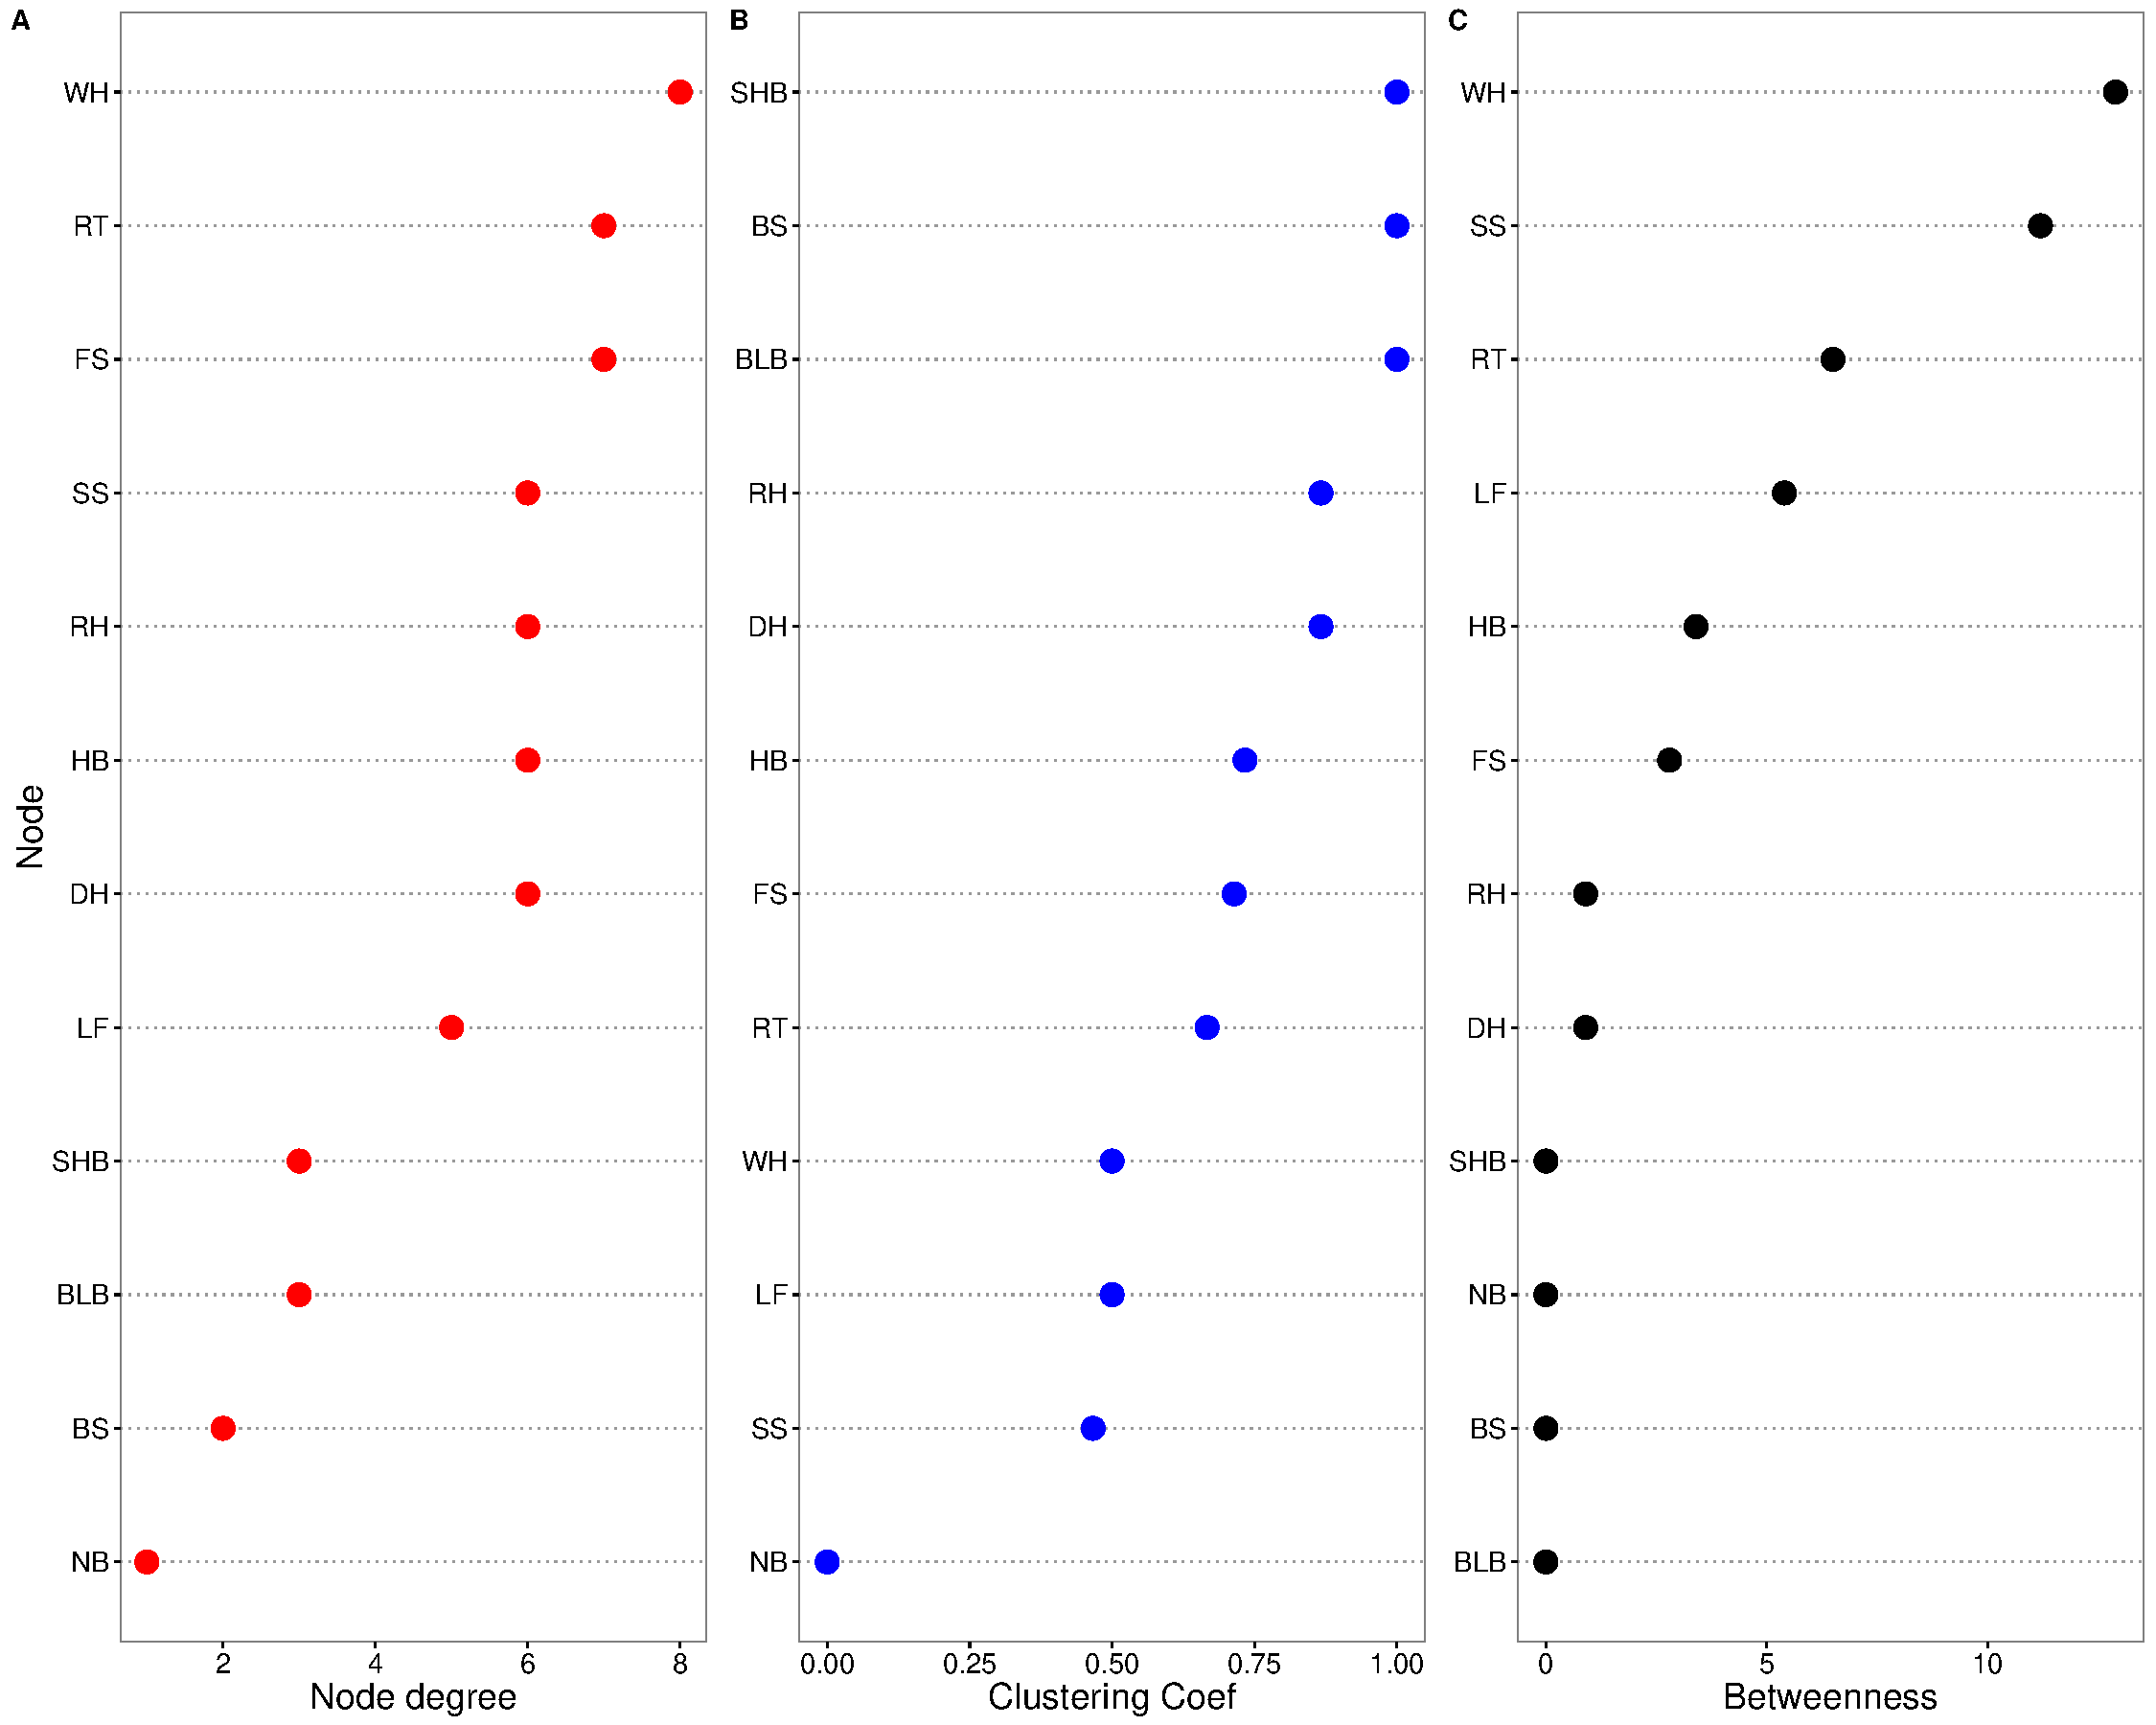
\includegraphics[width = 1\textwidth]{figures/nodepropTM_ws/nodepropTM_ws.pdf}
        \caption{Three centrality measures of the nodes in co-occurrence network of rice injuries in wet season at Tamil Nadu, India. A: node degree, B:clustering coefficient, and C:Betweenness, and.}
        \label{fig:nodepropTM_ws}
    \end{subfigure}
    \caption{Rice injuries in wet season in Tamil Nadu, India}
    \label{fig:TM_ws}
\end{figure}

\paragraph{West Java, Indonesia}

Co-occurrence network of injury profiles of dry season presented in Figure \ref{fig:networkWJ_ds}. The network reveals the four groups of injury profiles. Group1 (green) and group3 were close and group2 and group4 had less connection than others. Because of the structure and clustering coefficient, group1 and group3 are more likely to have chance to form association between the groups, and form complex association within group than between groups

Network in wet season (Figure \ref{fig:networkWJ_ws}) injuries and 54 associations. From the structure of this network, there were three type of injury syndromes.  One (group1; green) composed of SHB, RT, DH, RH, BLS, and SHR.  Within this group, BLS seems to be inducers (high betweenness), and SHB was connecter (high node degree). Two is combination of BS, LF, WM, NBS, and LM. This combination was clear that BS was dominant, and dominantly observed. Three is the combination of PM, RB, and FS. 

\begin{figure}
    \centering
    \begin{subfigure}[b]{1\textwidth}
        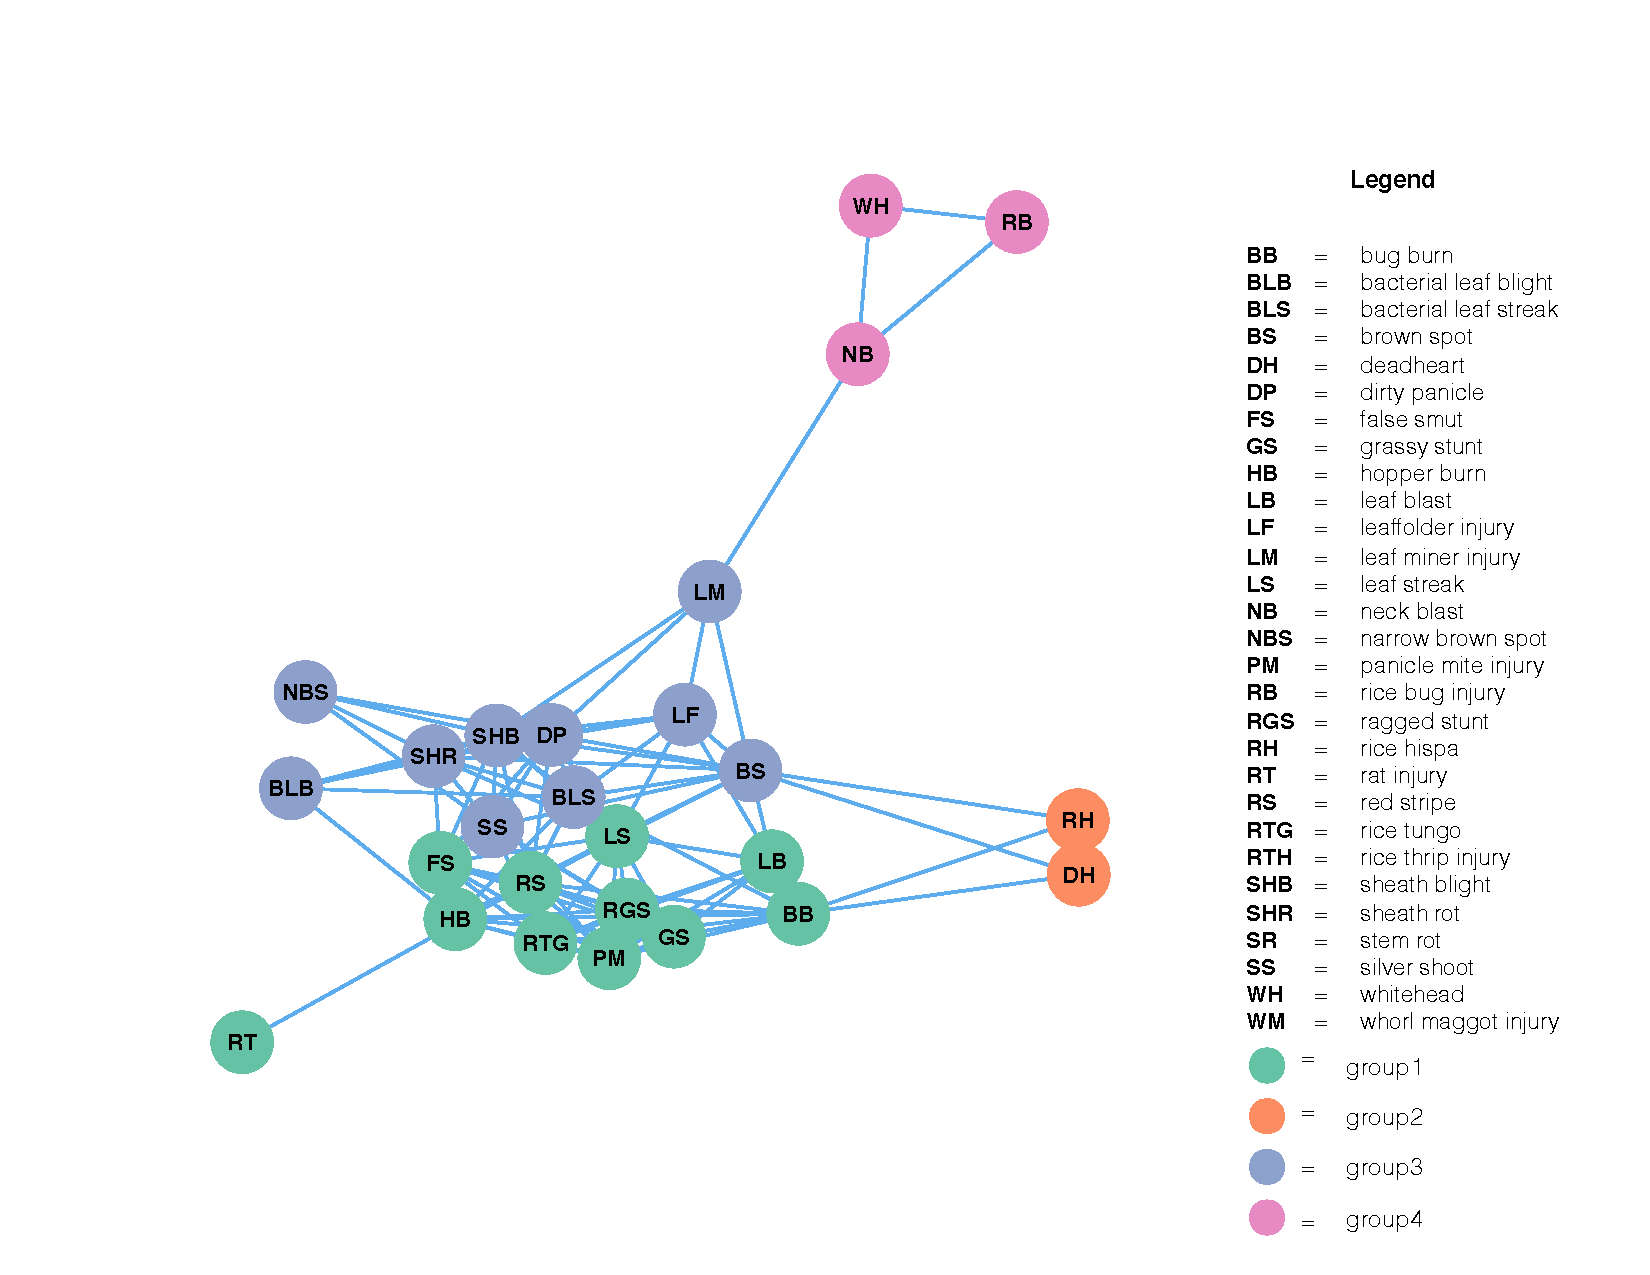
\includegraphics[width = 1\textwidth]{figures/networkWJ_ds/networkWJ_ds.pdf}
        \caption{Co-occurrence network of rice injuries in dry season at West Java, Indonesia. The layout of the network graph is based on the Fruchterman-Reingold algorithm, which places nodes with stronger or more connections closer to each other.}
        \label{fig:networkWJ_ds}
    \end{subfigure}
    \begin{subfigure}[b]{1\textwidth}
        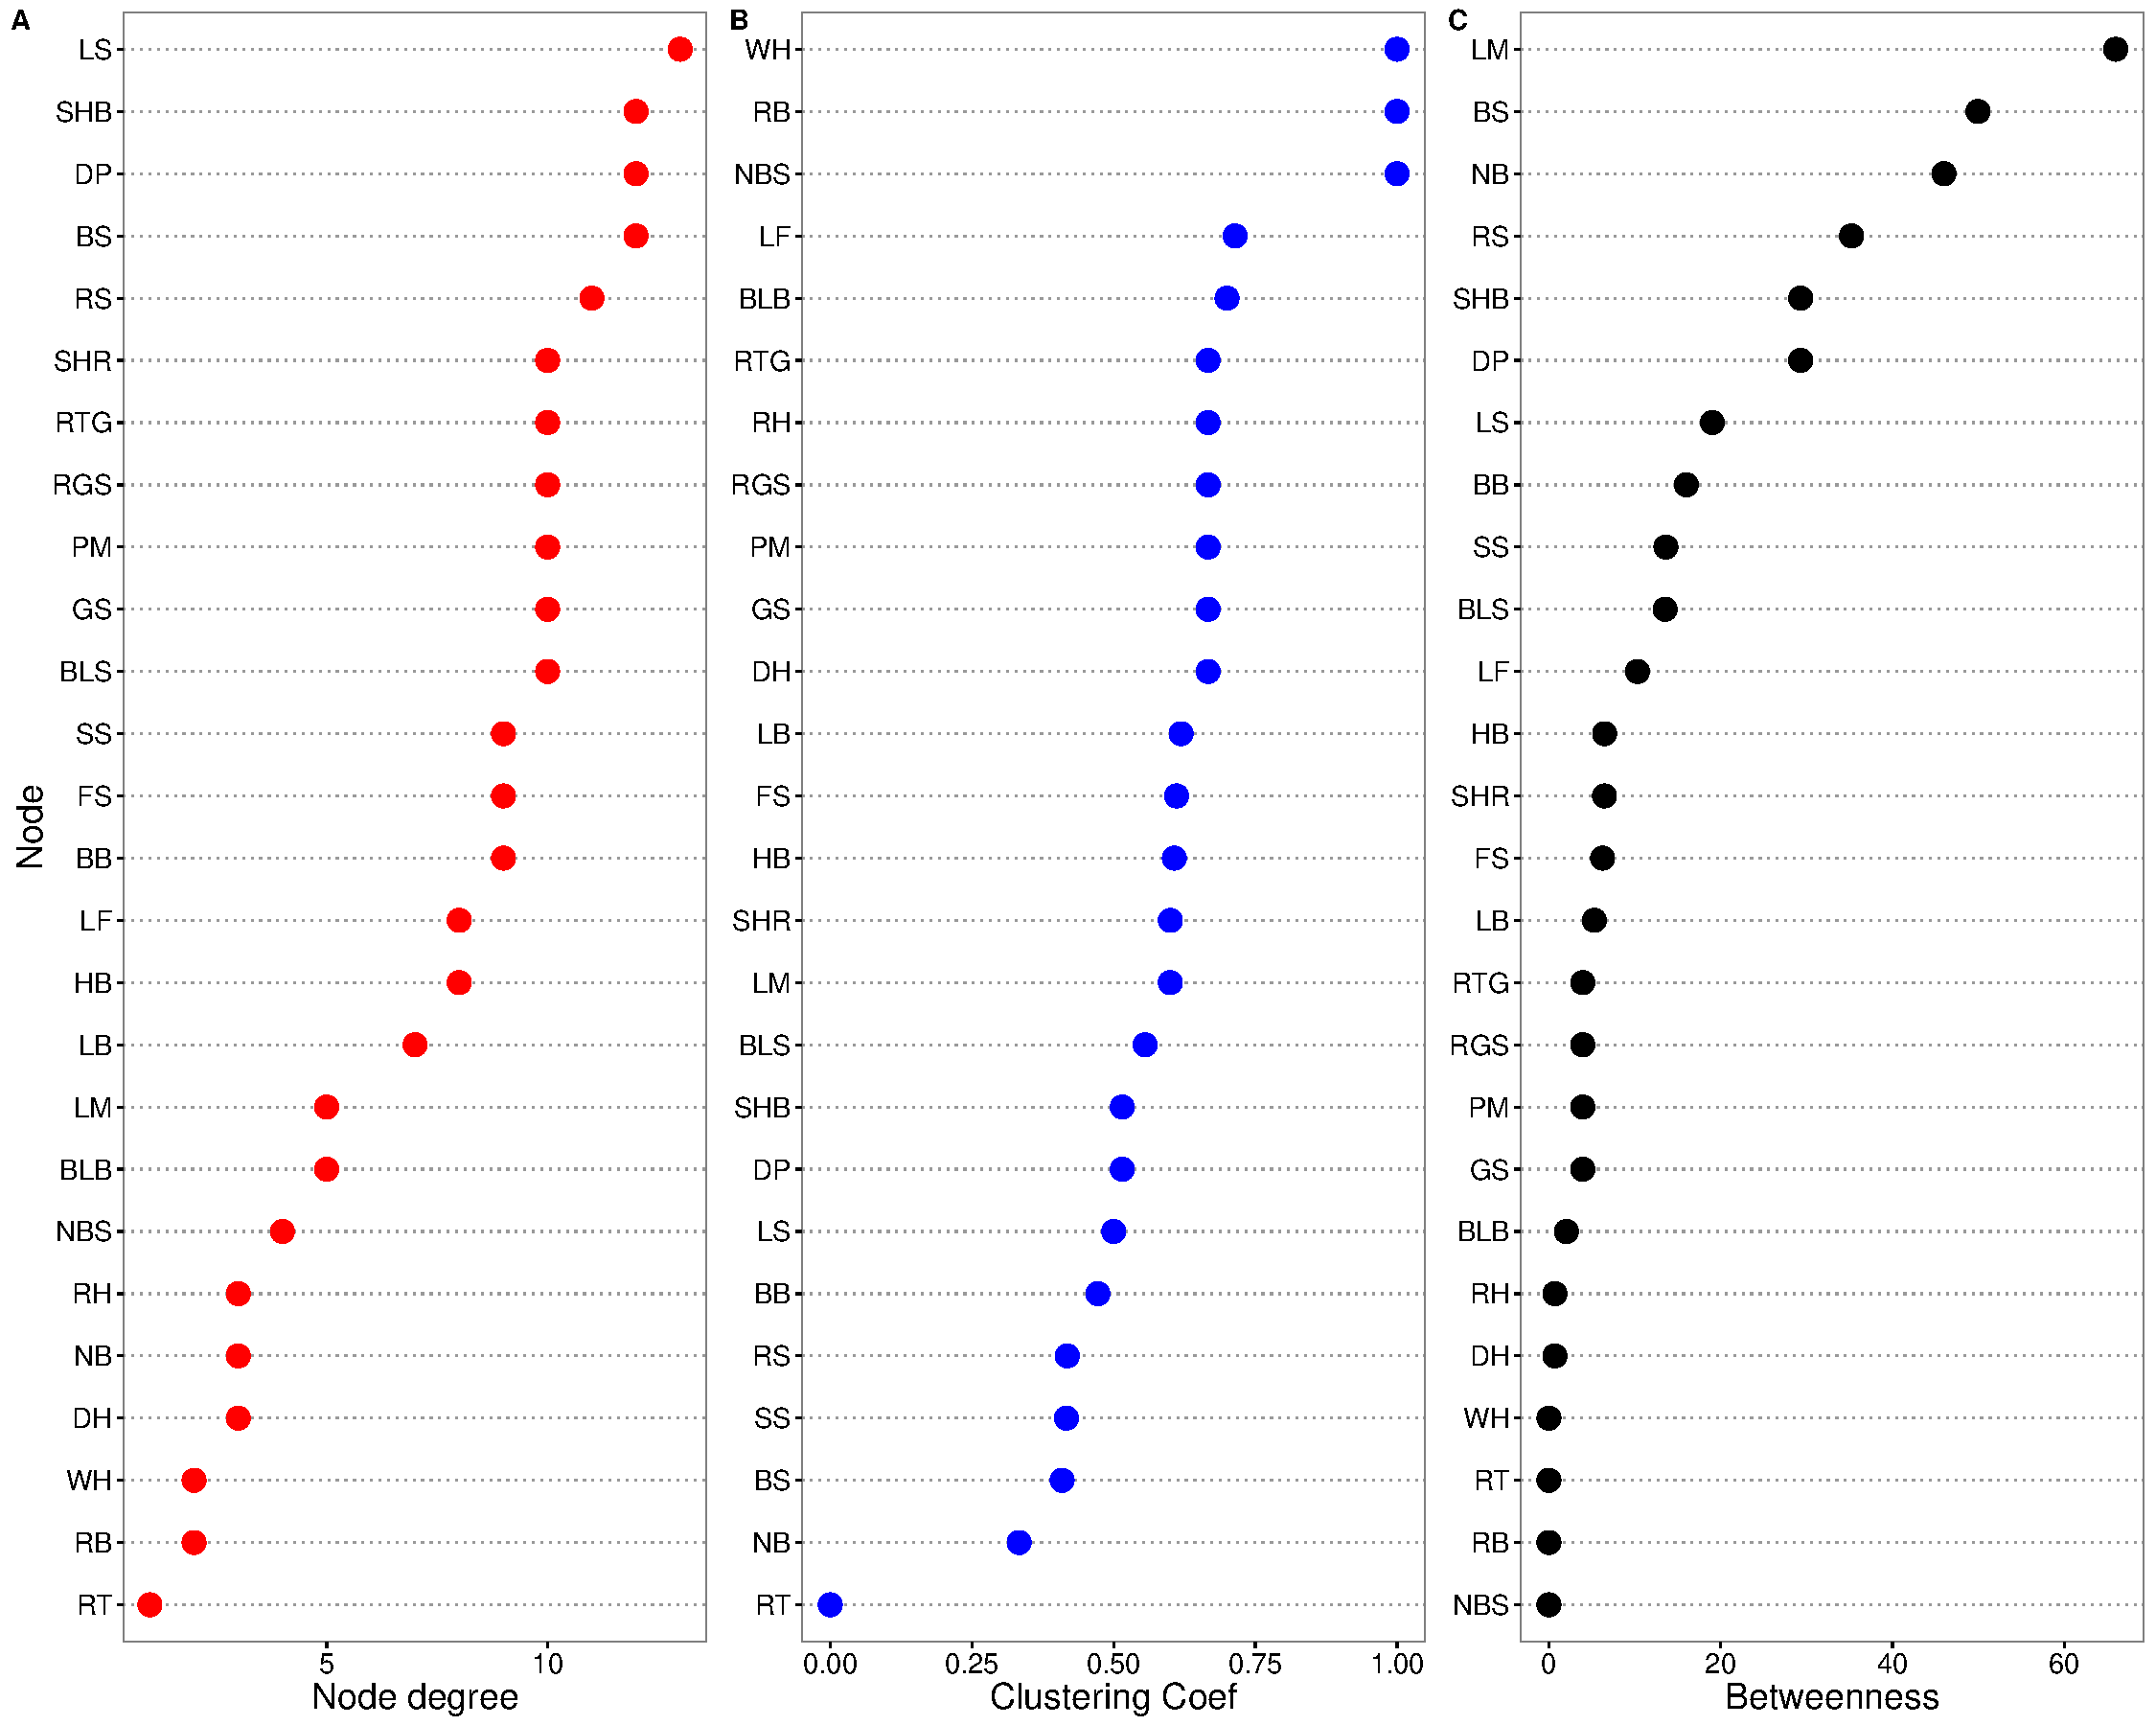
\includegraphics[width = 1\textwidth]{figures/nodepropWJ_ds/nodepropWJ_ds.pdf}
        \caption{Three centrality measures of the nodes in co-occurrence network of rice injuries in dry season at West Java, Indonesia. A: node degree, B:clustering coefficient, and C:Betweenness, and.}
        \label{fig:nodepropWJ_ds}
    \end{subfigure}
    \caption{Rice injuries in dry season in West Java, Indonesia}
    \label{fig:WJ_ds}
\end{figure}

\begin{figure}
    \centering
    \begin{subfigure}[b]{1\textwidth}
        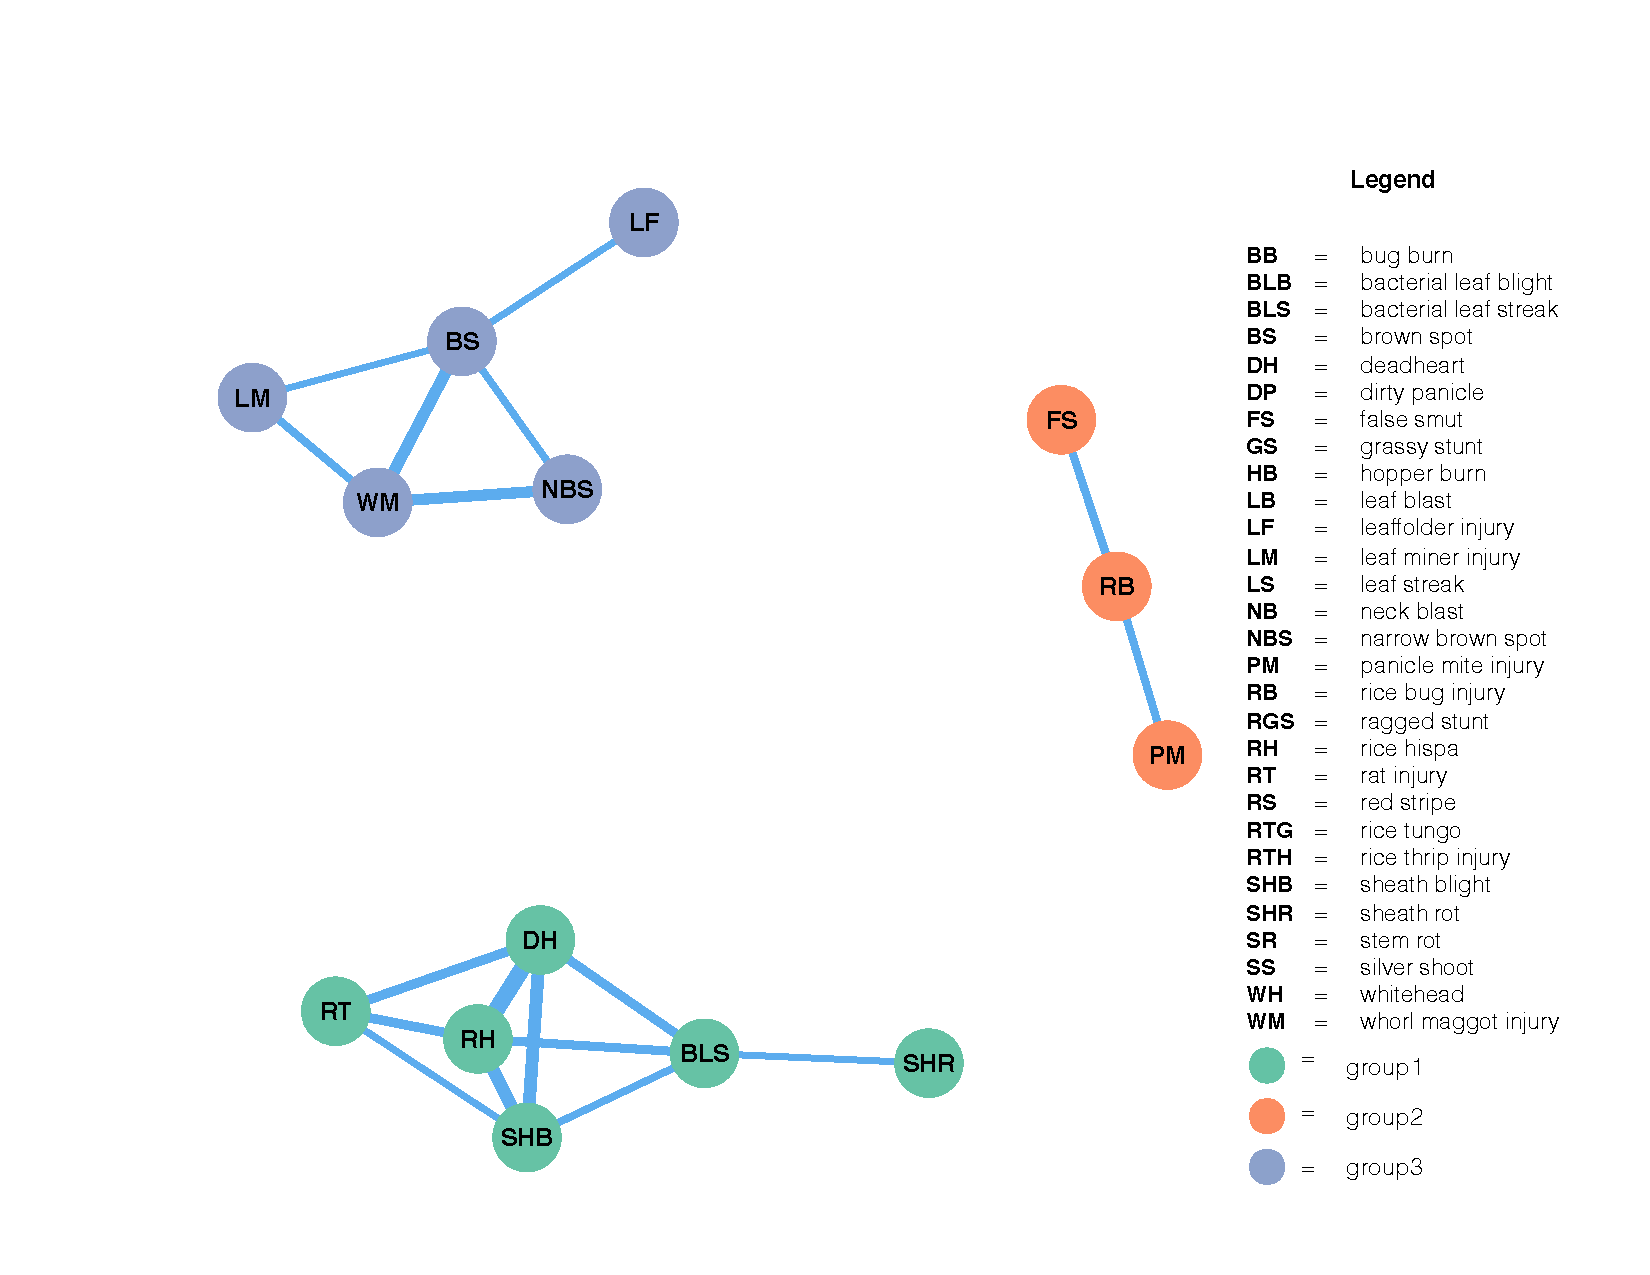
\includegraphics[width = 1\textwidth]{figures/networkWJ_ws/networkWJ_ws.pdf}
        \caption{Co-occurrence network of rice injuries in wet season at West Java, Indonesia. The layout of the network graph is based on the Fruchterman-Reingold algorithm, which places nodes with stronger or more connections closer to each other.}
        \label{fig:networkWJ_ws}
    \end{subfigure}
    \begin{subfigure}[b]{1\textwidth}
        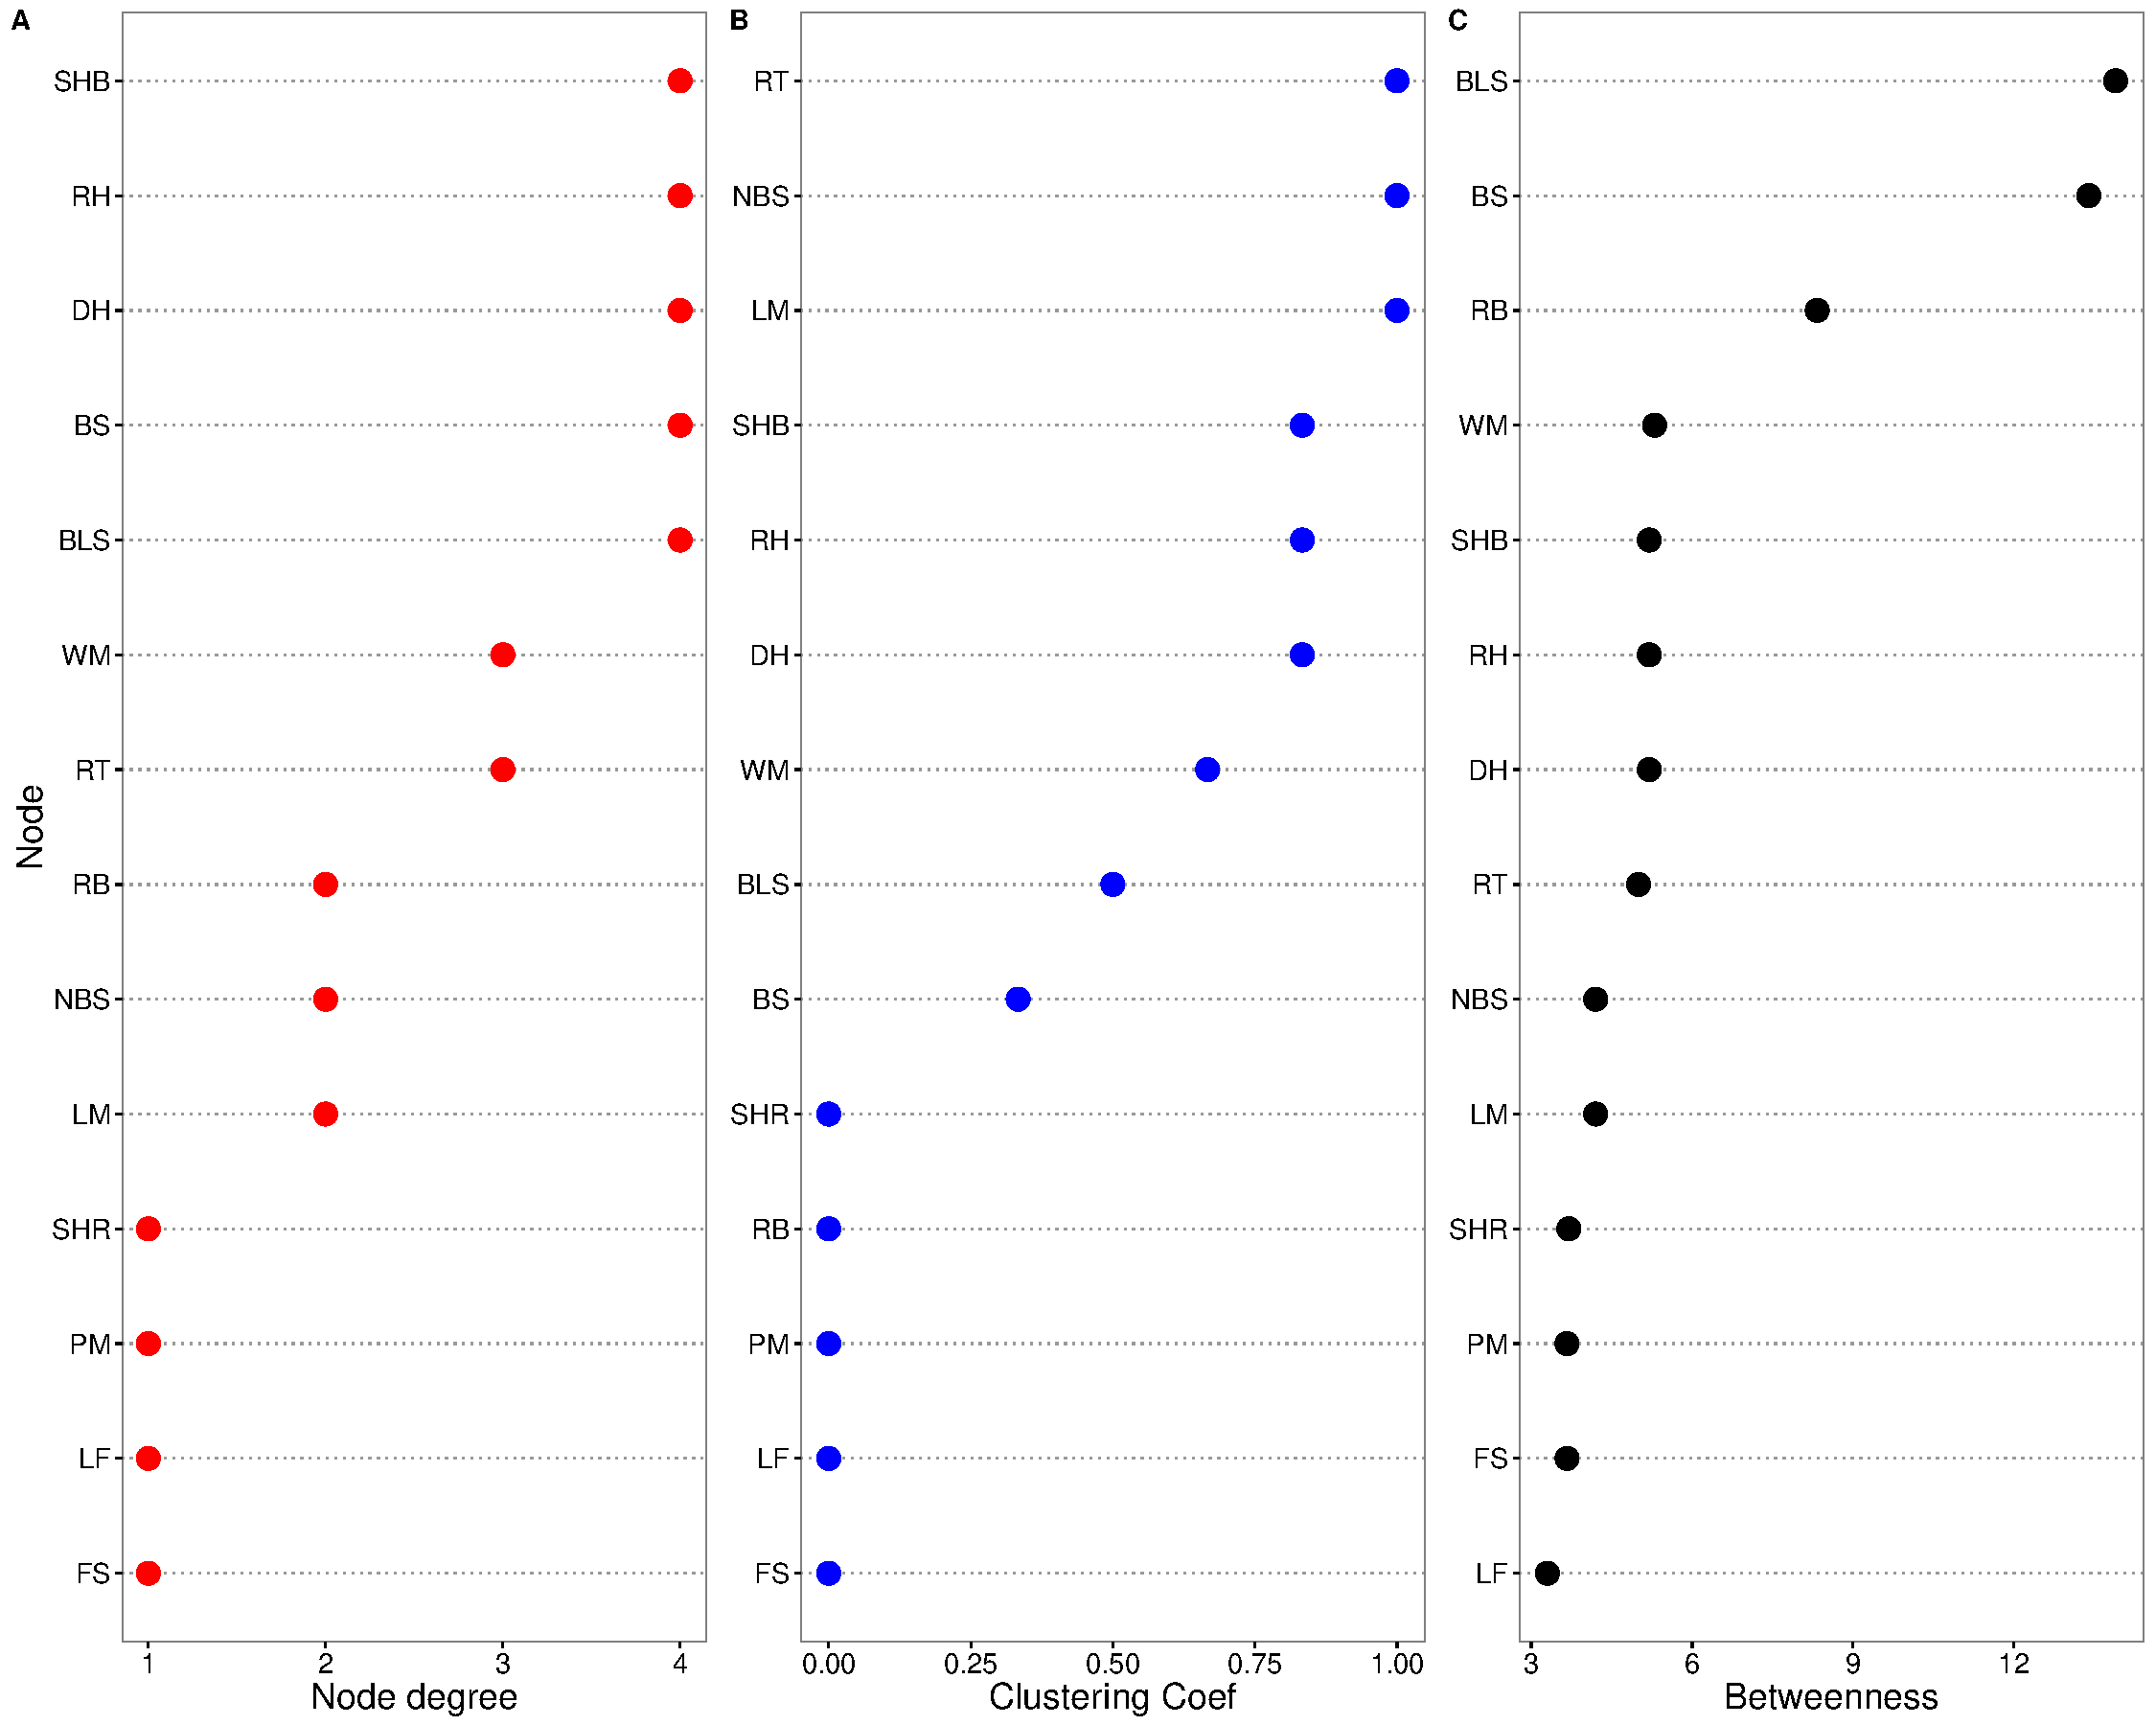
\includegraphics[width = 1\textwidth]{figures/nodepropWJ_ws/nodepropWJ_ws.pdf}
        \caption{Three centrality measures of the nodes in co-occurrence network of rice injuries in wet season at West Java, Indonesia. A: node degree, B:clustering coefficient, and C:Betweenness, and.}
        \label{fig:nodepropWJ_ds}
    \end{subfigure}
    \caption{Rice injuries in wet season in West Java, Indonesia}
    \label{fig:WJ_ws}
\end{figure}


\subsection{Discussion}
Even some nodes are less connected they may occuren in some season and not related to other and not fom co-ocurence

They may differul to preseict by suing other injuires 


Rice injuries were found commonly in South and South east Asia, but at different levels of incidence. 
Some injuries of this study is relatively low prevalence of areas that have been reported such as leaf blast, brown spot. It could be implied that these injuries strongly depended on locations or climatic conduction to develop, so they were not observed at all locations or seasons during survey were conducted. Another reason is that there are some factors such as the utility of resistance verities in the farmer’s fields surveyed, so we could observe those injuries at low level of incidence. The similar reasoning could explain to many injuries such as BLB, RB, NB, which widely occur in rice growing areas.

From the survey data of rice injuries observed in farmers’ fields, I analyzed the interaction and build the network based on that data. The methods applied for building a co-occurrence network of rice injuries were adapted from ecological studies. Usually, relationships were assessed using Pearson correlation. However, the use of the Pearson correlation coefficient is problematic because it requires the variables are applied with similar measure, and the variable values are normally distributed. Additionally, Pearson correlation can only capture linear relationships. Due to the fact that the assumptions of Pearson correlation are not fit with the survey data. The alternative is provided by using Spearman’s rank correlation coefficient, which is also widely used in ecological studies.

The exploration of co-occurrence networks is a useful method for determining interactions of co- occurring injuries. Network analysis has also suggested important injuries in networks. The important injuries were selected from the node features such as node degree, clustering coefficient, and betweenness. The betweenness represents the importance of the control potential that an injury exerts over the associations of other injuries in the network. The clustering coefficients are indicative of the potential spreading of the incidence of injuries through the network. As activated injury can activate other injuries, a more densely connected network facilitates injury activation \cite{Williams_2014_demonstrating}. In the network of dry season in West Java, Indonesia, BLB and SR can be the targets to be monitored because they have high betweenness, which indicated that they are more likely to present then others injuries.

It is good attempt to detect communities in a network because it can reveal information about the networks that is maybe not easy to detect by simple observation. The communities are groups of nodes that are densely connected among their node members, and slightly connected with the rest of the network.  In this study, we detected node community based on the optimization of the modularity of a sub-network, which is an approach that widely applied in many fields \cite{Liu_2014_Detecting}. Even though, the groups of injury profiles from this study are different from seasons and countries, but they are reasonable because some rice injuries present in some seasons (seasonal occurrence) such as gall midge injury \cite{Krishnaiah_2004_Rice}. The result also showed similar groups of injuries to the patterns of injuries profile from the study of \cite{Savary_2000_Characterization}. 

%SR is also best to be the target because it also associated with the RS, which has high clustering coefficients also because RS is potentially able to be co-found with many other injuries.  BLB also show the association with the injuries, which present high clustering coefficient. Both of BLB and SR are intermediate clustering coefficient., so they are formed concurrence between groups, but less potentially to present complex association. DH and WH are less associated with other injuries, so they are difficult to employ other injuries to. 

It is the good to monitored WM and RB  and SHB also even the GLH has no betweenness, but it has high clustering coefficients, and connected with two high betweenness node. It would be also good target to monitored also because when it present, it also frequency appear together.
We explored the characteristics of rice injury profiles

Communities are groups that are densely connected among their members, and sparsely connected with the rest of the network. Community structure can reveal abundant hidden information about complex networks that is not easy to detect by simple observation. 

With regard to pest management development, understanding that the relationships of rice injuries could simplify pest management decisions. As applied here, the node degree, clustering coefficients, and betweenness described the interaction of injuries in the networks. Therefore, they may be useful in finding a good indicator for monitoring pest in rice fields. High-betweenness node High- clustering coefficient node 

Community structure in complex network can reveal hidden information about complex networks that is maybe not easy to detect by simple observation such as nodes, which are clustered. In this study, we detected node community based on the optimization of the modularity of a sub-network, which is a popular approach \cite{Liu_2014_Detecting}. Even though, the groups of injury profiles from this study are different from seasons and countries, but they are reasonable because some rice injuries present in some seasons (seasonal occurrence) such as gall midge injury \cite{Krishnaiah_2004_Rice}. from the groups of injury profile from \cite{Savary_2000_Characterization}. 



\subsection{Conclusion}


%\chapter{Differential networks reveal the dynamics of animal pests and disease co-occurrences}
\chapter{Differential networks reveal the dynamics of animal injury and disease co- occurrences}

\subsection{Introduction}
Rice (\textit{Oryza sativa}) is a major crop in South and Southeast Asian. The Food and Agriculture Organization of the United Nations (FAO) estimates that approximately 70 percent of total lowland rice area produces tow rice crops each year. The first crop is cultivated in the wet season, while another is in the dry season. The important role of seasonal cropping in the temporal dynamics of animal pests and diseases has been studied under farmers field survey in South and Southeast Asia by the use of multivariate techniques \citet{Savary_2000_Characterization, Willocquet_2008_Simulating}. These studies showed that injuries profiles (the combination of injuries) differ from season to season due to weather patterns, which in dry season, crop losses were lower than in the wet season because of lower incidence and severity of pests and diseases \citep{Litsinger_1991_Crop}. Additional a previous study based on surveys done in farmers’ rice fields in the region of lowland rice were shown that injury profiles were strongly associated with season.

In the previous chapter, the co-occurrence networks showed  co-occurrence networks, a methodological approach which has already proved fruitful in a variety of different applications.  Plant injuries caused by pests maybe affect yield production. Therefore, in this chapter, I attempted to characterize the patterns of rice injuries by studying the changes in the co-occurrence patterns of rice injuries (\textit{e.g} disease incidence, animal pest injury incidence) in different season and different yield levels.

Differential network analysis aims to compare the connectivity of two nodes at two different conditions. As demonstrated by several studies, differential networks can identify important nodes implicated in my fields, and also provide critical novel insights not obtainable using other approaches. In this work, I explore the the properties of network of a complex association of rice injuries at different yield levels. Elucidating the rice injuries association represents a key challenge, not only for achieving a deeper understanding of injury association (injury profiles) but also for identifying the unique association. Given that the injury association is governed by a complex network of injuries association, it seems natural to explore network properties which may help elucidate some of different association presenting in the different seasons.

In this chapter, I employ a differential network topology method to examine the co-occurrence relationships of rice injuries from survey data. I use graph theory methods to examine the topological feature dynamic of a co-occurrence network corresponding to different seasons, and production environments. The co-occurrence networks were built from differentially co-occurring injuries. I extract significantly differential co-occurring injuries from co-occurrence networks, which represent different seasons, to identify which injuries that may be involved specifically curtain season. I postulate that these selected injuries may contribute to the difference in the co-occurrence patterns in different season. Furthermore, I identified the injuries associated with yield from networks at different yield levels. Finally, I suggest key injuries that may contribute to yield reduction under a curtain production environment. The goal is to leverage insights to better understand the rice injury co-occurrence that may contribute to pest management development.

\newpage
\subsection{Materials and Methods}

\textbf{Differential co-occurrence network construction}

The survey data were pre-processed by using methods described in the previous chapter. Subsequently, I applied the method proposed by \citet{Fukushima_2013_Diffcorr} to identify differentially co-occurrence links. The difference of co-occurrence of injury $x$ and $y$ between two conditions ($A$ and $B$) was quantified by Fisher's $z$-test.
 
For the pair of $x$ injury and $y$ injury, I denoted the correlation coefficient based on Spearman's correlation coefficient by $r_{xy}^A$ and $r_{xy}^A$ in networks of condition $A$ and condition $B$, respectively. To test whether the 2 correlation coefficients were significantly different, correlation coefficients for each of the 2 conditions, $r_{xy}^A$ and $r_{xy}^B$, were transformed into $Z_{xy}^A$ and $Z_{xy}^B$, respectively.


The Fisher's transformation of coefficient $r_{xy}^A$ is defined by
\begin{equation}
\label{eq:zvalue}
Z_{xy} = \frac{1}{2} \log\left[{\frac{1 + r_{xy}}{1 - r_{xy}}}\right]
\end{equation}

Next, The $p$-value of the difference in $Z_{xy}$ values was calculated using the standard normal distribution.

\begin{equation}
\label{eq:pofz}
p(Z\geq \left | \frac{Z_{xy}^A - Z_{xy}^B}{\sqrt{\frac{1}{N_{A}-3}+ \frac{1}{N_{A}-3}}} \right |
\end{equation}

Next, The $p$-value of the difference in Z values was calculated using the standard normal distribution

$N_{A}$ and $N_{A}$ represent the sample size for each of condition. The $Z$ has an approximately Gaussian distribution under null hypotheses that the population correlations are equal. The pairwise correlation significants are considered at $p$-value < 0.05.


\textbf{Differential co-occurrence network in different seasons}

Consider any two injuries $x$ and $y$ in the survey data, let $r_{xy}^D$ and $r_{xy}^W$ be the Spearman’s correlation coefficient calculated separately over the samples in dry and wet, respectively. I constructed differential co-occurrence networks that are specified by adjacency matrix $A^{diff}$ = $(A_{xy}^{diff})$ where the entry $A_{xy}^{diff}$ quantified by following:   


\begin{equation}
A_{xy}^{diff} = \left\{\begin{matrix}
 1 & \text{when } r_{xy}^D > r_{xy}^W \text{ at } P_{z_{xy}} \text{-value}  < 0.05  \\ 
 0 & \text{when } P_{z_{xy}}  \text{-value}  > 0.05                              \\ -1 & \text{when } r_{xy}^W > r_{xy}^D \text{ at } P_{z_{xy}} \text{-value}  < 0.05 \end{matrix}\right.\end{equation}


For this differential co-occurrence network,$A_{xy}^{diff}$ equals 1 depending on whether any injury pairs show significantly higher correlation coefficient of co-occurrence  in dry season than wet season, but -1 is vice versa, and if it equal 0, meaning that co-occurrence level of injury pairs were not different in dry and wet season. \ref{fig:pipeline3} illustrated the differential co-occurrence network at different seasons.

\begin{figure}[h]
\centering
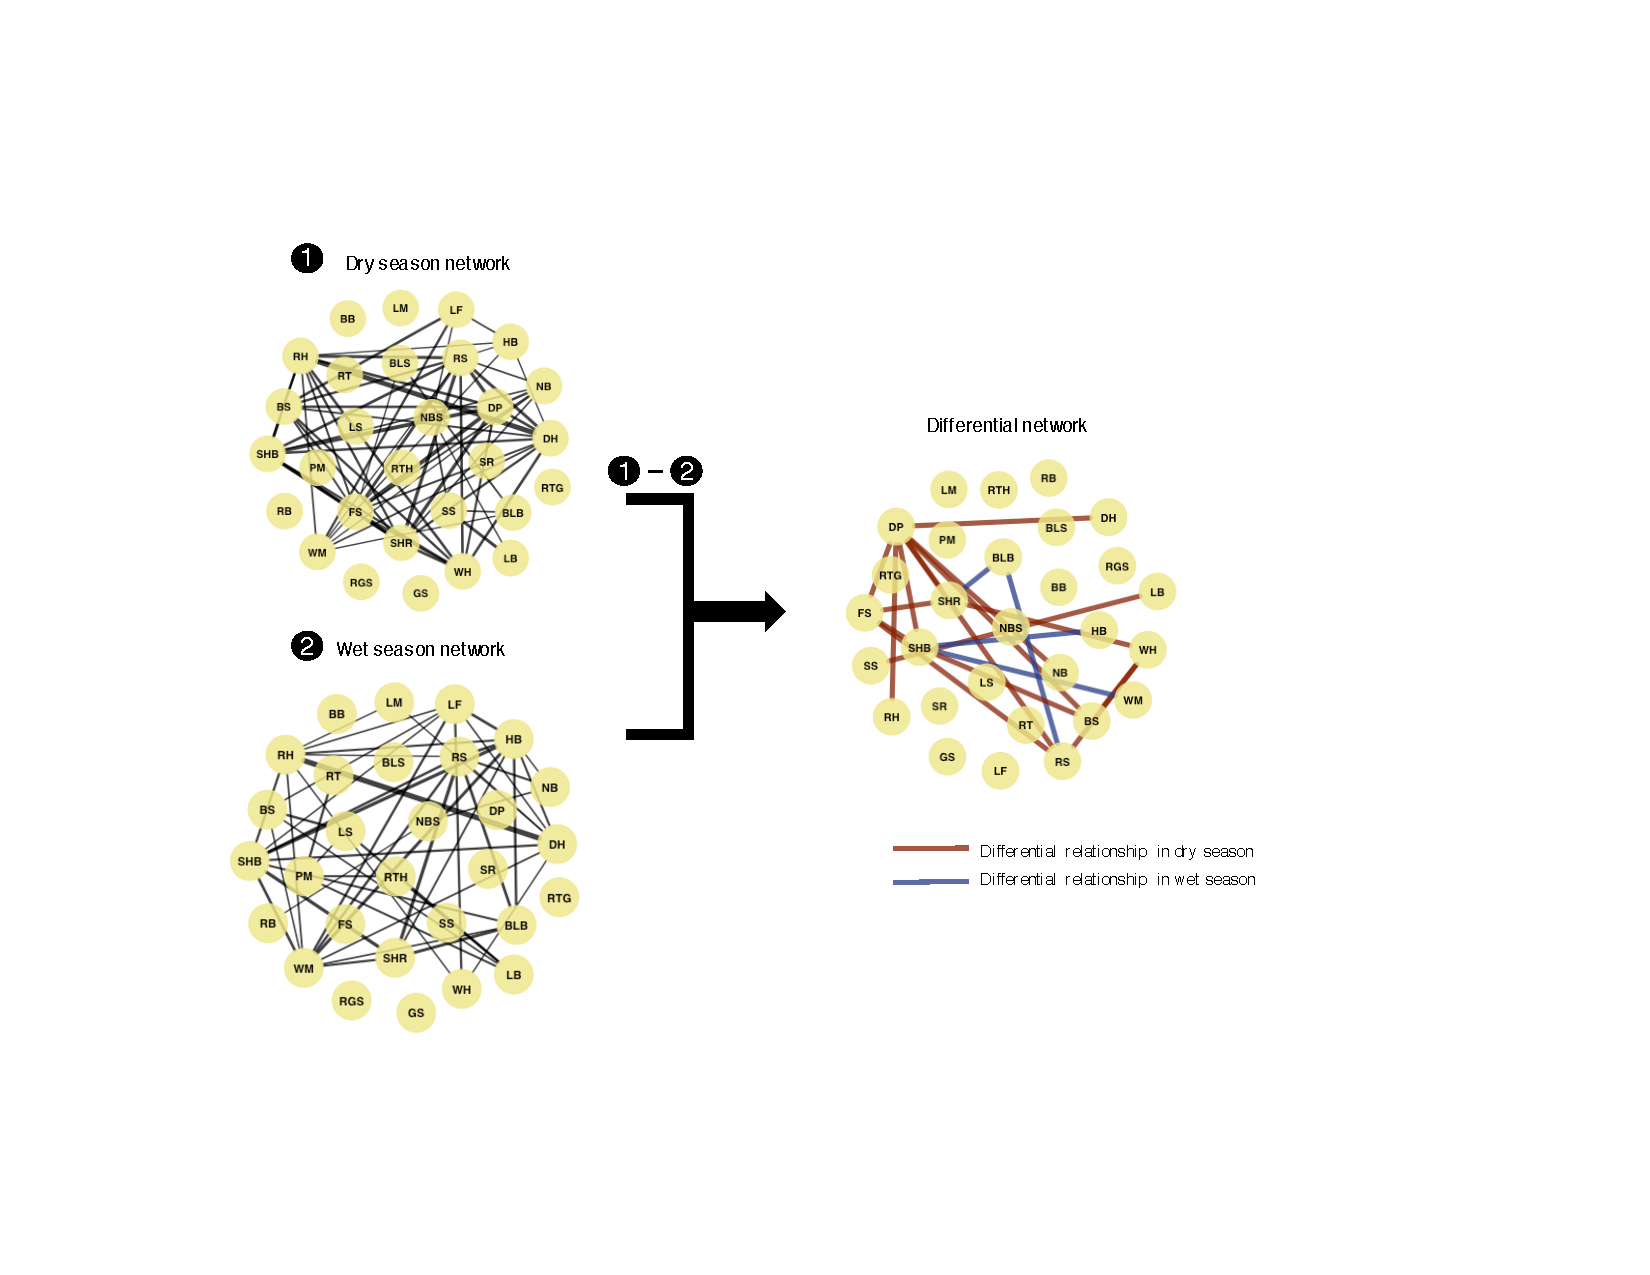
\includegraphics[width = 1\textwidth]{figures/pipeline3.pdf}
\caption[Differential analysis of crop health survey data in season]{Schematic showing differential analysis in seasons. Co-occurrence networks are measured in each of two seasons (left) resulting in interactions (black). Dry season is subtracted from wet season to create a differential co-occurrence network (right), in which the significant differential interactions are those that positive (red) or negative (blue) in score after the shift in conditions, which means differential in dry, and wet season, respectively.}
\label{fig:pipeline3}
\end{figure} 

\textbf{Difference of co-occurrence network of rice injuries at different yield levels}

Consider any two injuries $x$ and $y$ in the survey data, let $r_{xy}^L$ and $r_{xy}^H$ be the Spearman’s correlation coefficient calculated separately over the samples in $L$ and $H$ yield level, respectively. I constructed differential co-occurrence networks that are specified by adjacency matrix $A^{diff}$ = $(A_{xy}^{diff})$ where the entry $A_{xy}^{diff}$ quantified by following:   

\begin{equation}
A_{xy}^{diff} = \left\{\begin{matrix} 1 & \text{when } r_{xy}^L > r_{xy}^H \text{ at } P_{z_{xy}} \text{-value} < 0.05  \\  0 & \text{otherwise}                             
\end{matrix}\right.
\end{equation}

For  this differential co-occurrence network,$A_{xy}^{diff}$ equals 1 depending on whether any injury pairs show significantly higher co-occurrence level in low yield level than high yield state, and if it equal 0, meaning that co-occurrence level of injury pairs were not or lower different in low yield level state. \ref{fig:pipeline4} illustrated the differential co-occurrence network at different seasons.

\begin{figure}[h]
\centering
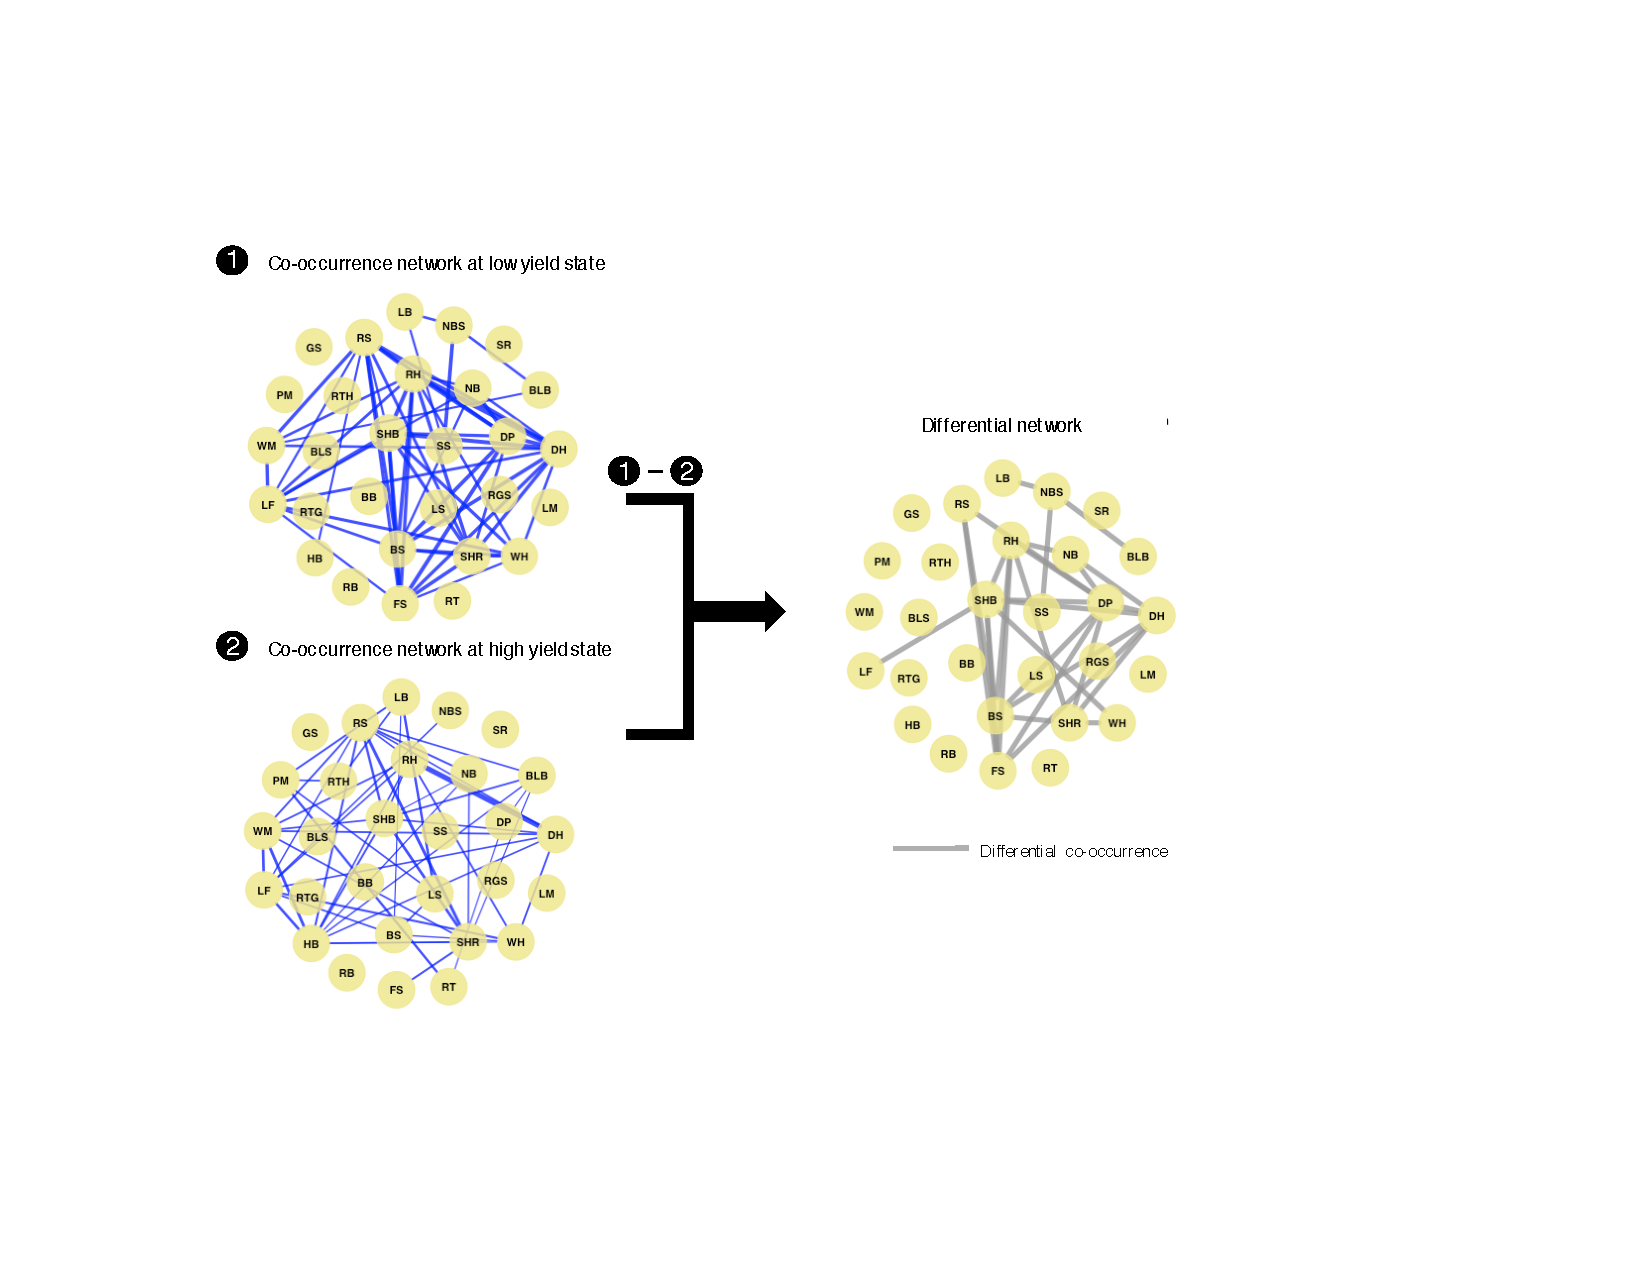
\includegraphics[width = 1\textwidth]{figures/pipeline4.pdf}
\caption[Differential analysis of crop health survey data at different yield levels]{Schematic showing differential analysis at different yield levels. Co-occurrence networks are measured in each of two different yield levels (left) resulting in interactions (blue). The network at low yield level network is subtracted from high yield level to create a differential co-occurrence network (right), in which the significant differential interactions are those that positive in score after the shift from low to high yield state.}
\label{fig:pipeline4}
\end{figure} 

\textbf{Topological properties}
To investigate the structural properties of differential networks, I calculated topological features for each node in the network with the \textbf{igraph} package. This feature set included node degree, clustering coefficient, and betweenness. 


\clearpage
\subsection{Results}

Differential network approach to constructing response networks enables easy comparison of the generated graphs. This, in turn allowed identification of the differences between the responses of co-occurrence relationships of rice injuries. In particular, in the differential network, I identified injuries and network components that are relevant for responsive condition as well as responsible for condition. 


\subsubsection{Construction of differential co-occurrence networks of rice injuries at different seasons}

I determined differential co-occurrence patterns of rice injuries of survey data in dry and wet season. The Differential co-occurrence network in season (DCONS), presenting pairs of injuries (nodes) connected with significantly different co-occurrence relationships (edges), are showed in \ref{fig:difseasonCP} - \ref{fig:difseasonWJ}. DCONS at Central Plain (Figure. \ref{fig:difseasonCP}) reveals SHB, SHR, and RS showing significantly different co-occurrence in both dry and wet season. They are likely to observed theses injuries. DP, SHB are high-betweenness in this network. Obviously, DP are likely to be observed in dry season because there are many pathway to increase it. Also, SHB  


   var degree betweenness clust.coef
1   RH      1    0.000000        NaN
2   SS      1    0.000000        NaN
3   WH      3    1.750000  0.0000000
4   DH      1    0.000000        NaN
5   DP      8   36.750000  0.1428571
6   FS      4    4.750000  0.5000000
7   NB      1    0.000000        NaN
8   WM      1    0.000000        NaN
9  BLB      2    0.250000  0.0000000
10  BS      3    4.333333  0.3333333
11  LB      1    0.000000        NaN
12  RS      4    6.833333  0.1666667
13  HB      1    0.000000        NaN
14 SHB      5   21.500000  0.2000000
15 SHR      4    6.833333  0.1666667


DCONS at OD \ref{fig:difseasonOD} reveals LB different both in dry and wet season. The group of injuries that present in wet season are RH, SS, FS, DH, and LM. But in dry season, there are SHB, BS, WH, NB.

var degree betweenness clust.coef
1   RH      2         0.0  1.0000000
2   SS      3         0.5  0.6666667
3   DH      2         0.0  1.0000000
4   FS      3         0.5  0.6666667
5   NB      1         0.0        NaN
6   LM      1         0.0        NaN
7   WM      1         0.0        NaN
8   BS      2         1.0  0.0000000
9   LB      2         1.0  0.0000000
10 SHB      1         0.0        NaN

DCONS at RR \ref{fig:difseasonRR} reveals that DP, BS, RTH, LF. 

PM- NBS in wet season , GS-BB-BLS in dry season

var degree betweenness clust.coef
1   WH      2          12          0
2   PM      1           0        NaN
3   DP      2          12          0
4  RTH      2           6          0
5   LF      2           6          0
6   WM      1           0        NaN
7  BLB      2          10          0
8  BLS      1           0        NaN
9   BS      2          10          0
10  LB      1           0        NaN
11 NBS      1           0        NaN
12  BB      1           0        NaN
13  GS      2           1          0

DCONS at TM shows two injury pairs express significantly co-occurrence in dry season, which are WH-BS, and DP-RTH, and one injury pair (SHB-LF) apparently occur together in wet season. 



DCONS at WJ (Figure.\ref{fig:difseasonnetwork_WJ} revealed that BS, NBS, SHB, and BLS co-occurring in both seasons.   

There are cluster group of injuries PM RS RTG RGS BB GS in dry season 

DP SHR

\ref{fig:difseasonTM}
   var degree betweenness clust.coef
1   RT      2   0.3333333  0.0000000
2   RH      3   5.6666667  0.0000000
3   WH      1   0.0000000        NaN
4   PM      5   0.2500000  0.9000000
5   RB      1   0.0000000        NaN
6   DH      3   5.6666667  0.0000000
7   DP      6   7.7500000  0.4666667
8   NB      1   0.0000000        NaN
9   LF      3   0.0000000  1.0000000
10  LM      1   0.0000000        NaN
11  LS      1   0.0000000        NaN
12  WM      2   0.5000000  0.0000000
13 BLB      3   1.0000000  0.6666667
14 BLS      4   4.8333333  0.1666667
15  BS      4   7.7500000  0.5000000
16 NBS      2   2.2500000  0.0000000
17  RS      4   0.0000000  1.0000000
18  BB      4   0.0000000  1.0000000
19  GS      5   0.2500000  0.9000000
20 RGS      5   0.2500000  0.9000000
21 RTG      5   0.2500000  0.9000000
22 SHB      7  27.1666667  0.2380952
23 SHR      6  14.0833333  0.4000000




\subsection{shared co-occurrence patterns networks of rice injuries at different season}

\begin{figure}
\centering
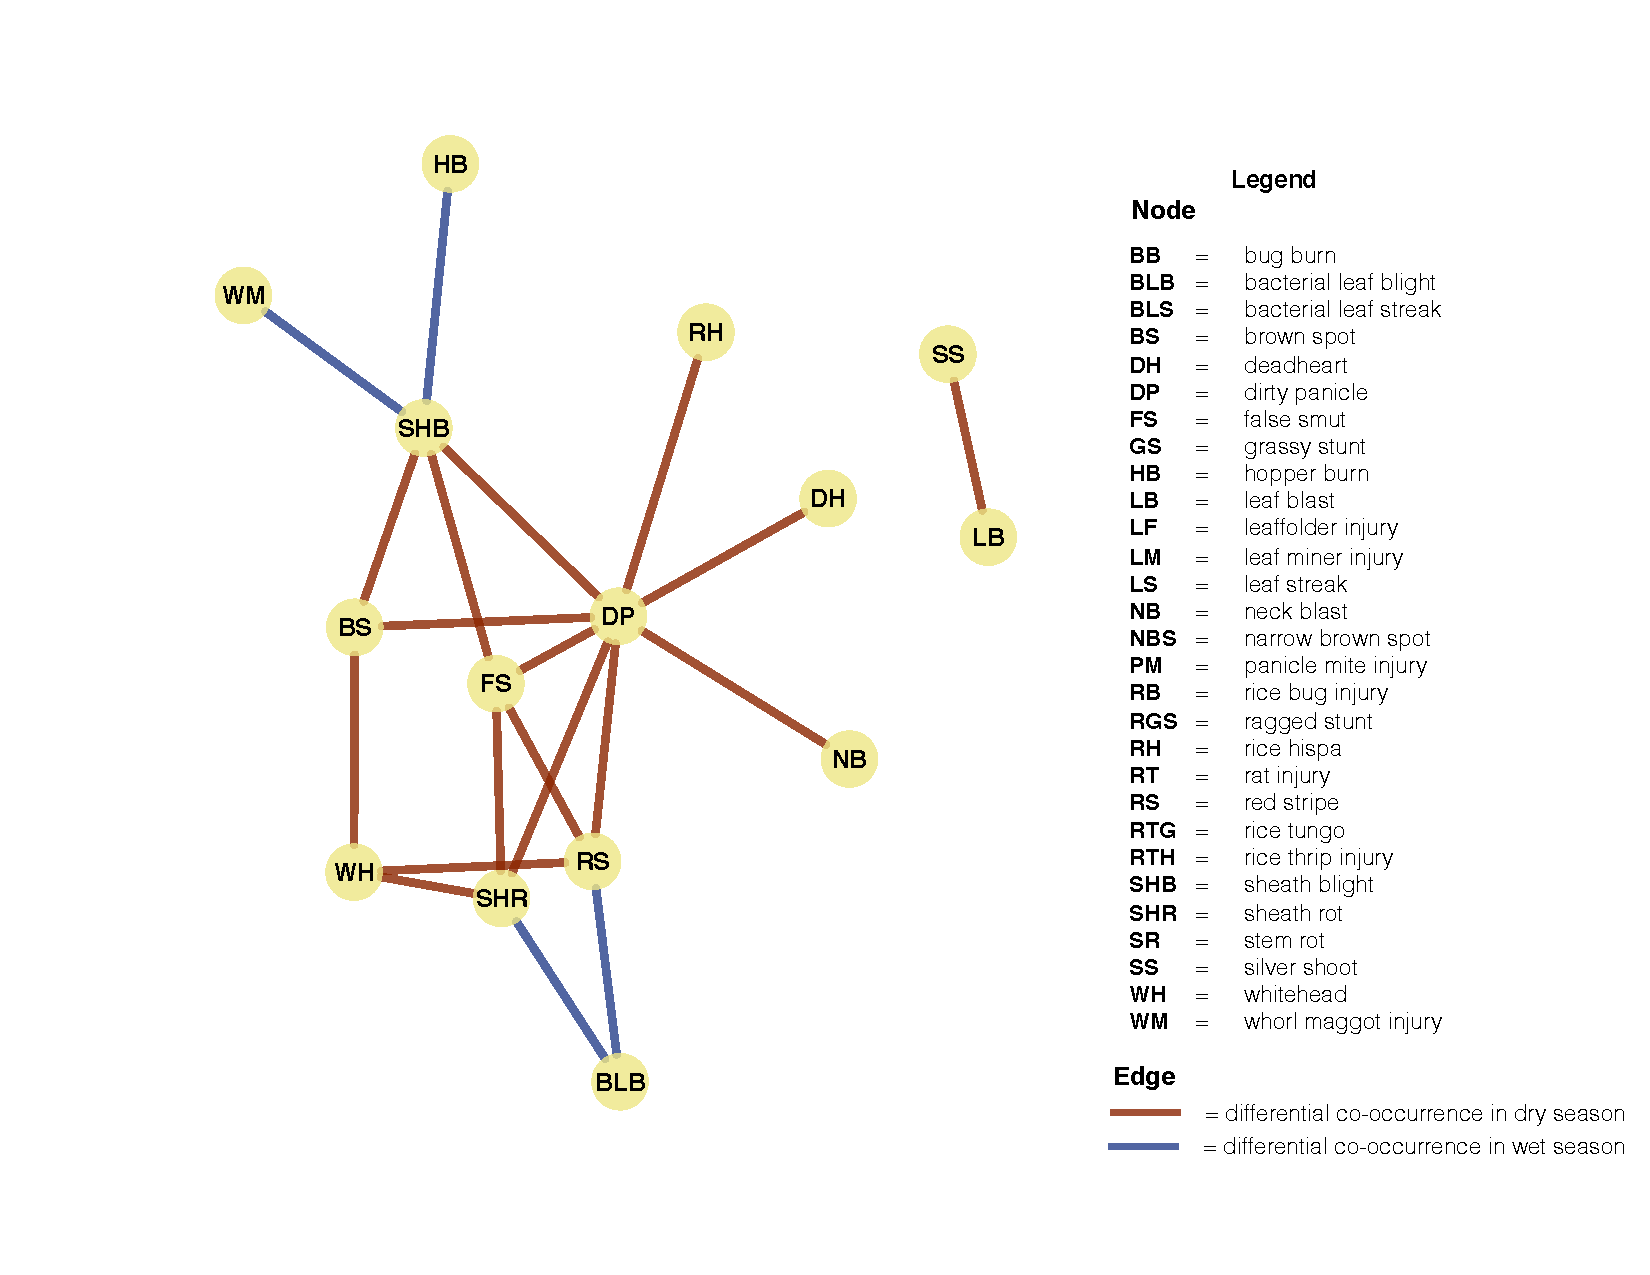
\includegraphics[width = 1\textwidth]{figures/difseasonCP.pdf}
\caption{Differential co-occurrence network of rice injuries in different seasons at Central Plain, Thailand}
\label{fig:difseasonnetwork_CP}
\end{figure} 

\begin{figure}
\centering
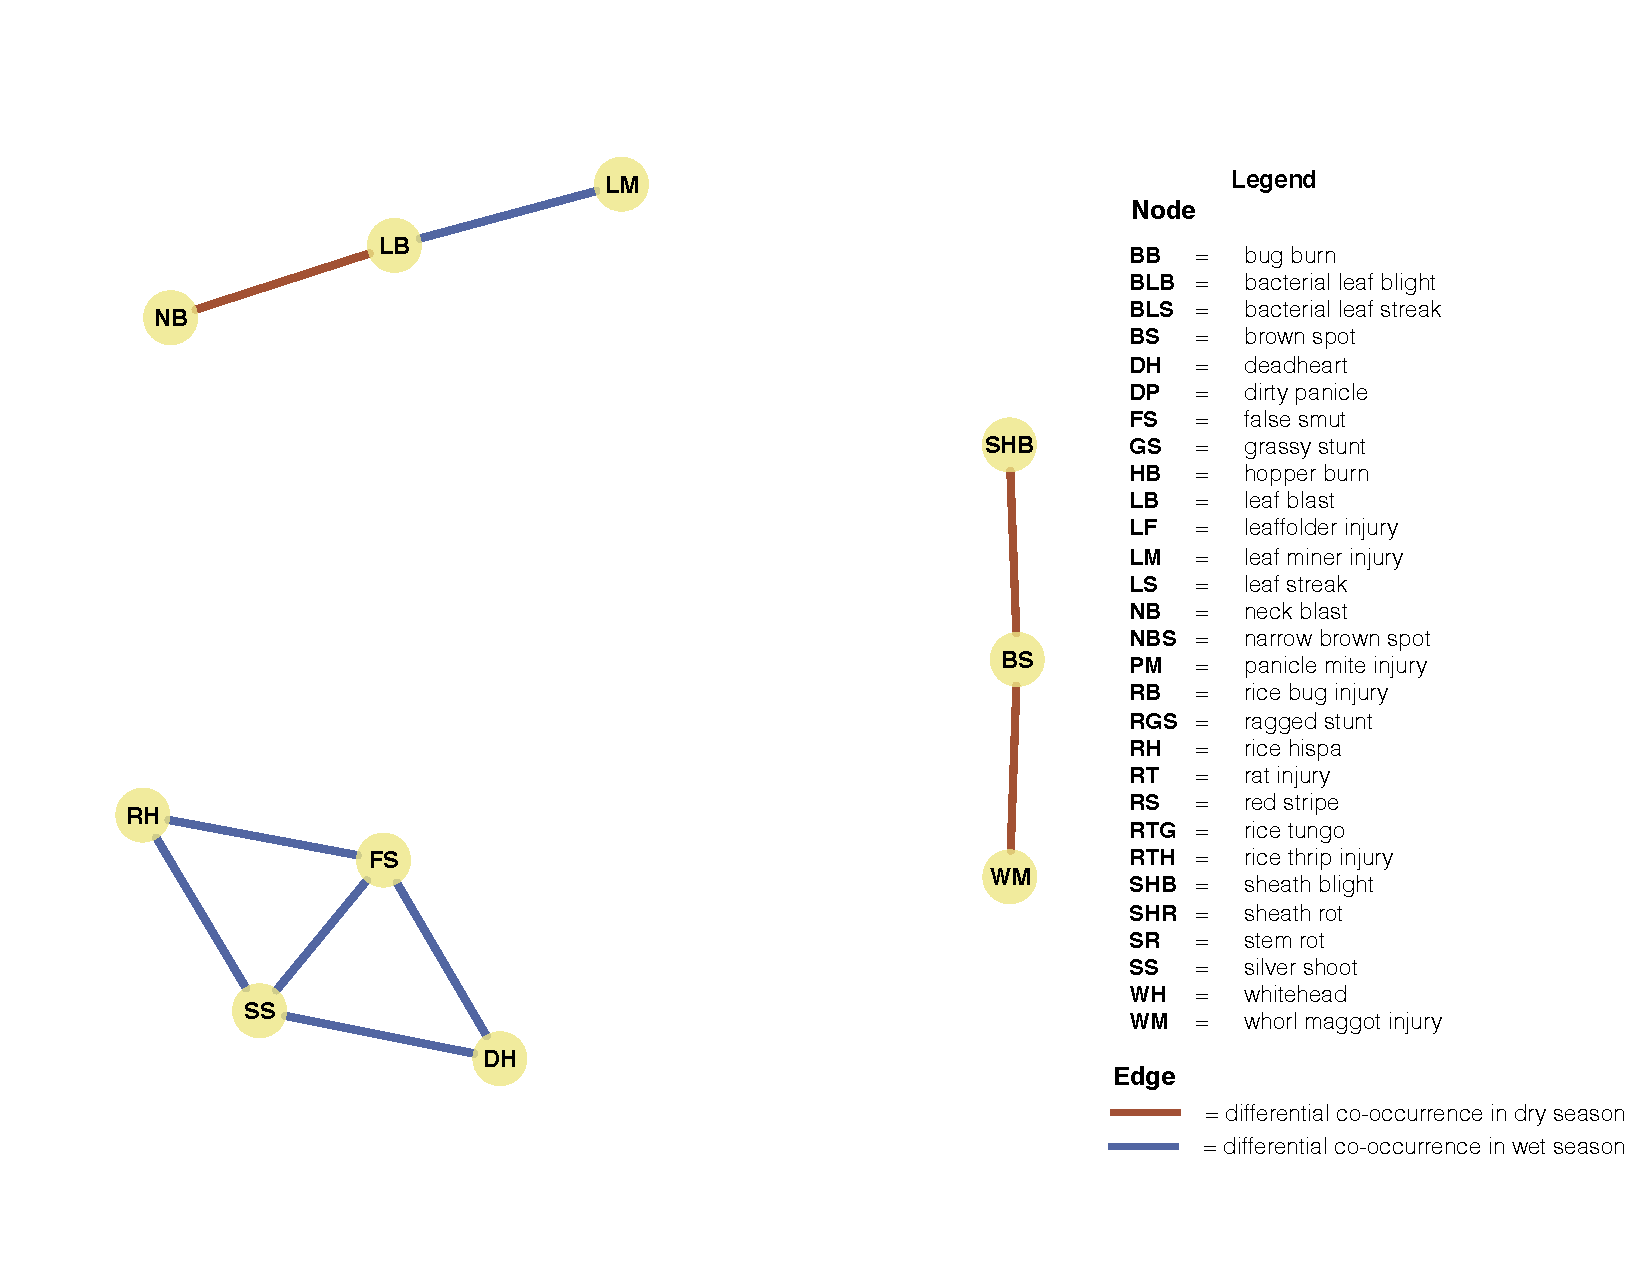
\includegraphics[width = 1\textwidth]{figures/difseasonOR.pdf}
\caption{Differential co-occurrence network of rice injuries in different seasons at Odisha, India }
\label{fig:difseasonnetwork_OR}
\end{figure}


\begin{figure}
\centering
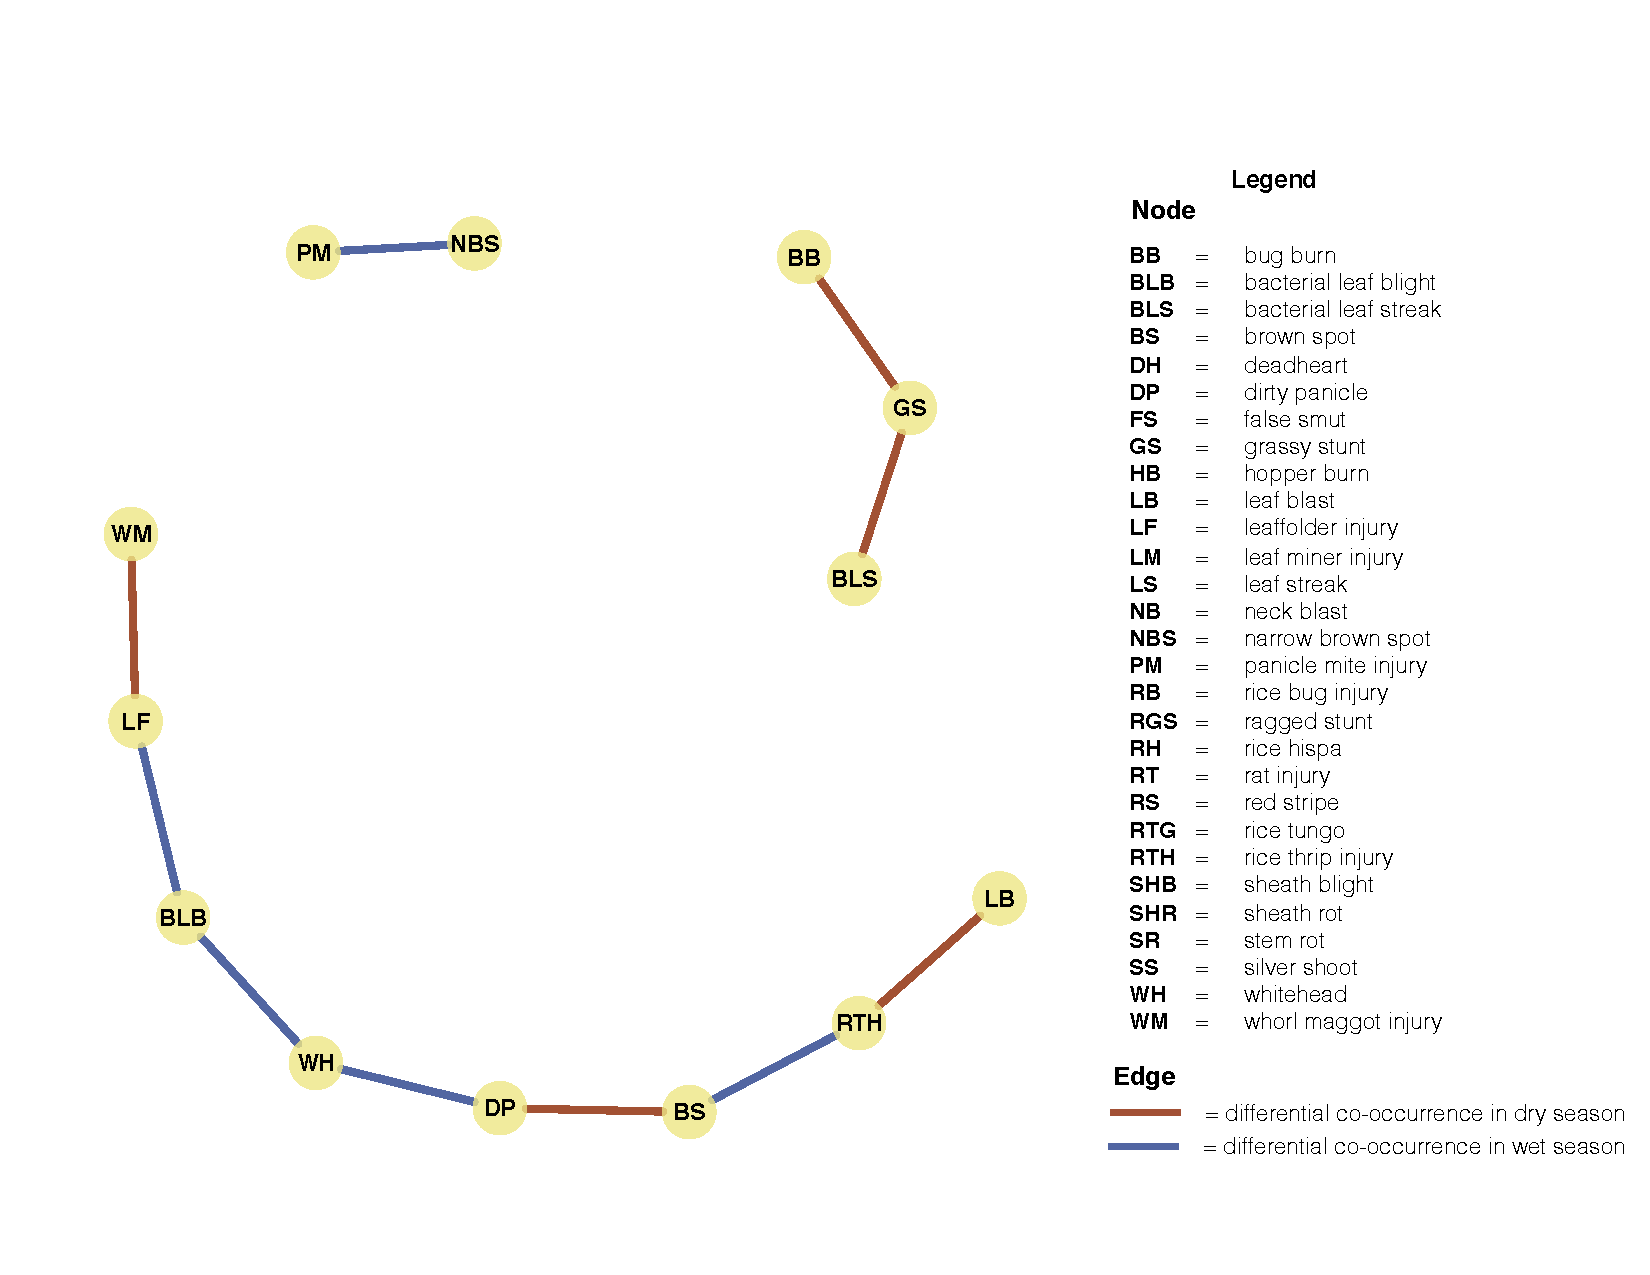
\includegraphics[width = 1\textwidth]{figures/difseasonRR.pdf}
\caption{Differential co-occurrence network of rice injuries in different seasons at Red River Delta, Vietnam}
\label{fig:difseasonnetwork_RR}
\end{figure}


\begin{figure}
\centering
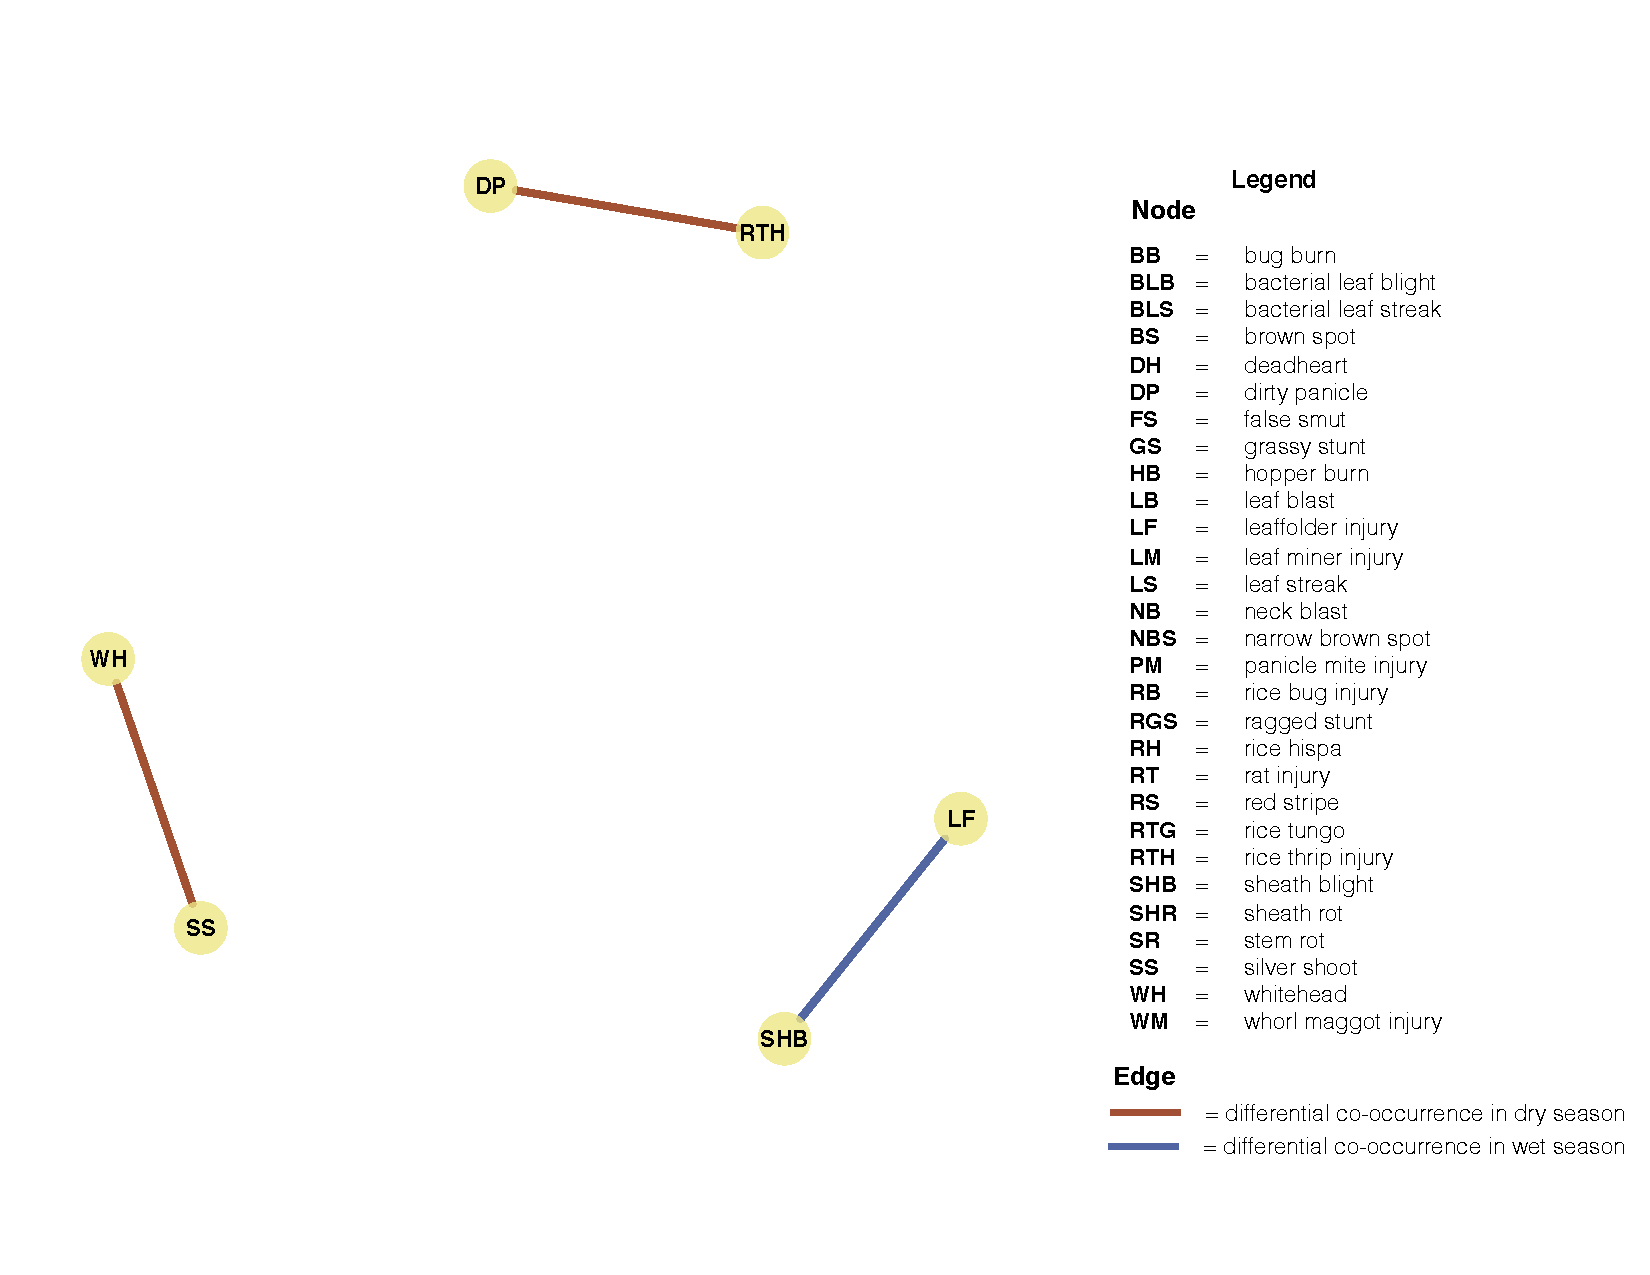
\includegraphics[width = 1\textwidth]{figures/difseasonTM.pdf}
\caption{Differential co-occurrence network of rice injuries in different seasons at Tamil Nadu, India}
\label{fig:difseasonTM}
\end{figure}


\begin{figure}
\centering
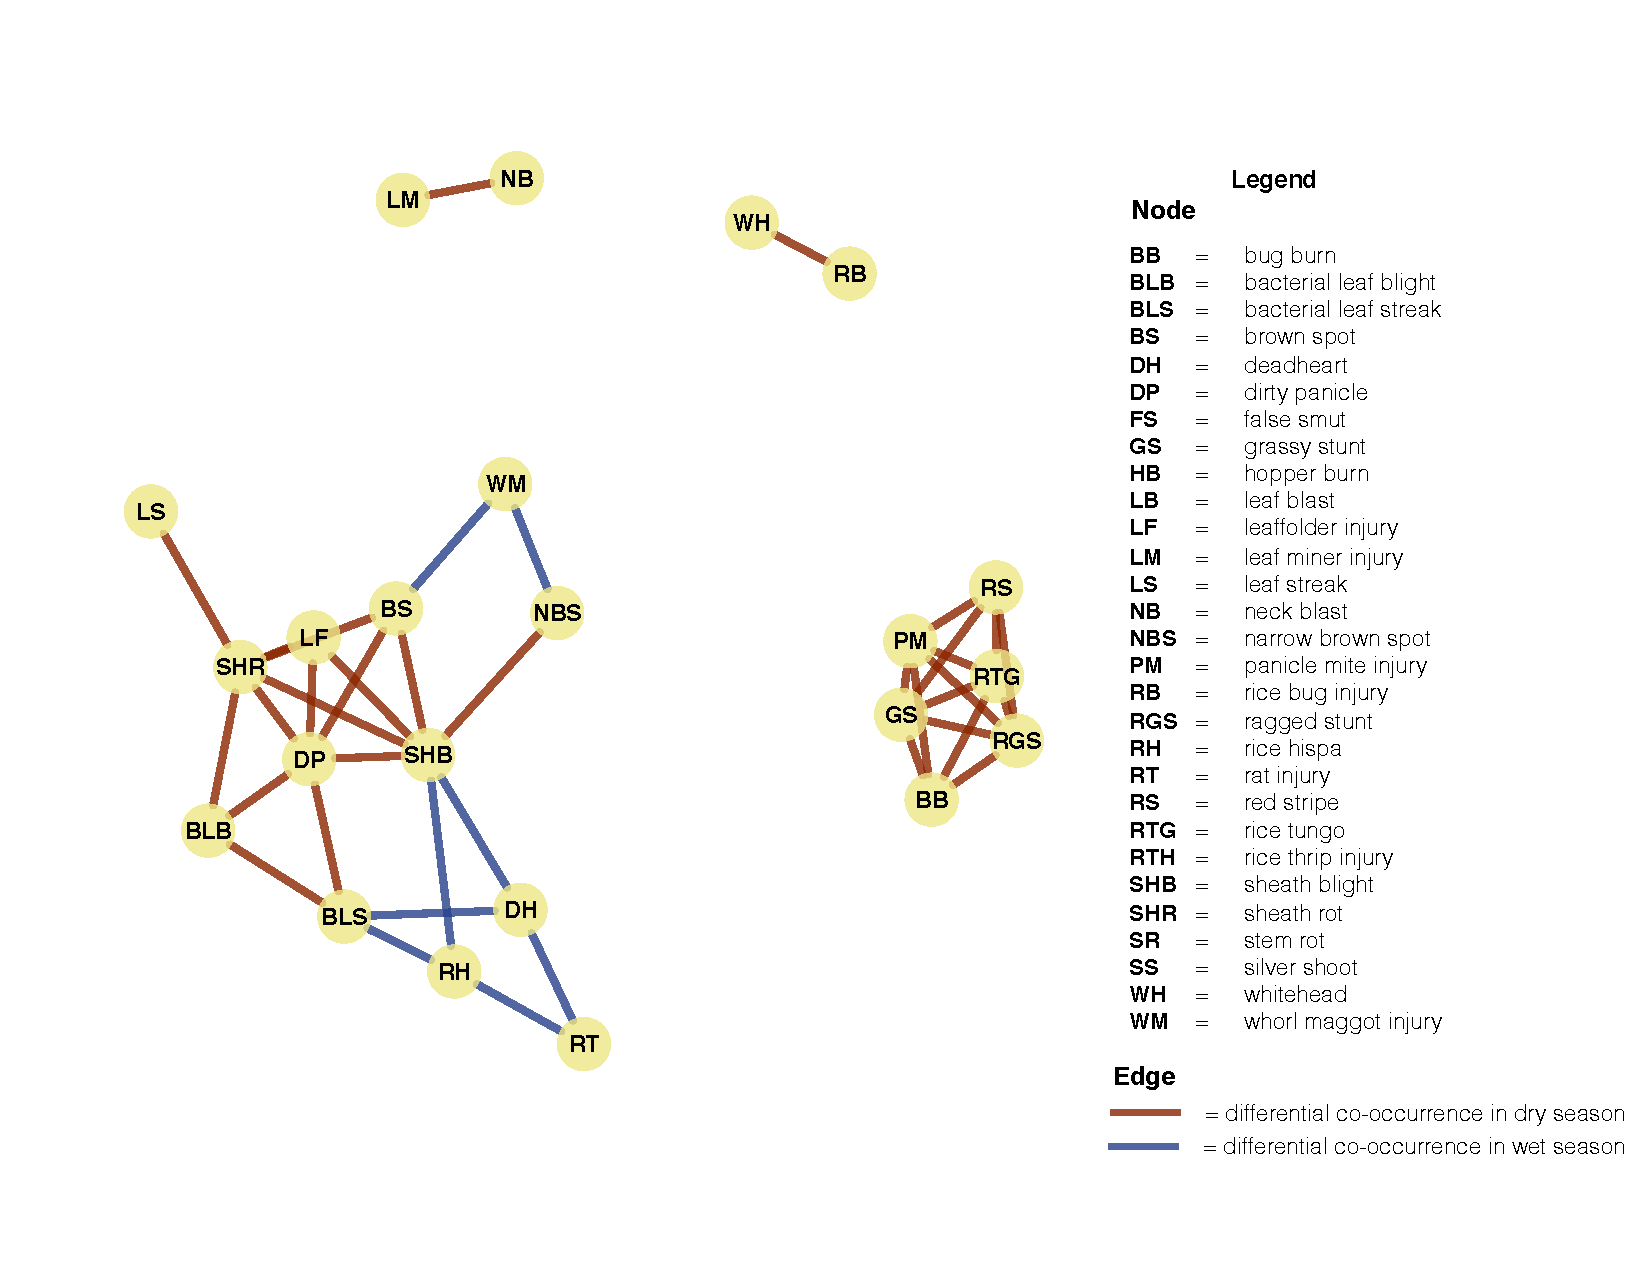
\includegraphics[width = 1\textwidth]{figures/difseasonWJ.pdf}
\caption{Differential co-occurrence network of rice injuries in different seasons at West Java, Indonesia}
\label{fig:difseasonWJ}
\end{figure}

%================================
\subsubsection{Differential co-occurrence networks of rice injuries at yield levels}

Comparison of the injury co-occurrence networks differed by season and the generic stress response network induced by different yield levels revealed features unique to each graph. In particular, I not only detected the presence of injuries, but I was able to see how they interacted with other genes in their respective networks. 
The injuries showed in the differential networks are the injuries showed co-occurrence patterns represented by edges. Edges were determined as co-occurrence correlation that express significantly higher in lower yield level. 

In this study, three successive yield classes were defined, in order to enable a better description of actual yield, from low (< 4 ton/ha), medium (4 – 6 ton/ha),  high (> 6 ton/ha) yield levels. Figure \ref{fig:yield_level_bar} shows the number of farmers’ fields surveyed classified in each season, and production environment.

\citet{Berry_2014_Deciphering} recommended that a co-occurrence network will be more reliable, it should be produced using a minimum of 25 samples or observations. From figure \ref{fig:yield_level_bar}, to be able compare the networks at different yield levels, I chose the data set, which are medium and high yield level of Central Plain, low and medium yield level of Odisha, medium and high yield level at Red River Delta, low and medium yield level of Tamil Nadu, and medium and high yield level of West Java. 

The resulted networks, differential co-occurrence network in yield (DCON-Y), depicts the associations of injury pairs significantly expressing in lower yield state but absent in higher yield state. Figures.\ref{fig:difyieldnetwork_CP} presents DCON-Y between medium and high yield level. It comprised of two groups of related injuries. Form node properties, DP, SHB, BS, RH, FS, and DH are high node degree and betweenness, which are likely to occur in this state because there are many connection, which can increase other injuries related, be induced by them as well. BS, SHB, are DP recorded in survey data showed these injuries were observed higher in medium than high yield data set(Fiure. \ref{fig:nodepropdifyield_CP}). DCON-Y compared between low yield and medium yield level at Odisha (Figure \ref{fig:difyieldnetwork_OD}) shows closely associated injures (DH, RH, FS, BS, WH). Their relationships were captured only in low yield state, and WH, BS, and FS are injuries connecting to all the injuries. Survey data also found that these injuries were observed in high frequency at high level of incidence (Figure \ref{fig:nodepropdifyield_OD}). In Red River delta, DCON-Y (Figure.\ref{fig:difyieldnetwork_RR}) reveals three injury combinations (DP-WH, GS-BB, and WM-LB-RTH) presenting in medium yield level, not in high yield level. So their co-occurrences may affect to yield losses between medium to high yield levels. Based on the survey data, DP, WM, and WH were found more incidence in low yield than high yield level (Figure. \ref{fig:nodepropdifyield_RR}). Apparently, in Tamil Nadu, Figure.\ref{fig:difyieldnetwork_TM} showed the co-occurrence pattern between SHB and WH that was found only in low yield level state, even though, from survey data, WH were found higher incidence in medium yield level than low yield level, but SHB were observe high incidence in low yield level than medium yield level (Figure \ref{nodepropdifyieldnetwork_TM}). In West Java, DCONY (Figure. \ref{fig:difyieldnetwork_TM}) reveals two groups of associated injuries that significantly express in medium yield level state. Form topological features of this DCON-Y, FS, RS, SHB, and LB are high betweenness nodes, which they are more likely to occur or be observed in this state because there are many pathway to increase them. SHB based on survey data also were highly found in medium than high yield level (Figure.\ref{fig:nodepropdifyield_WJ}).  

\begin{figure}
    \centering
        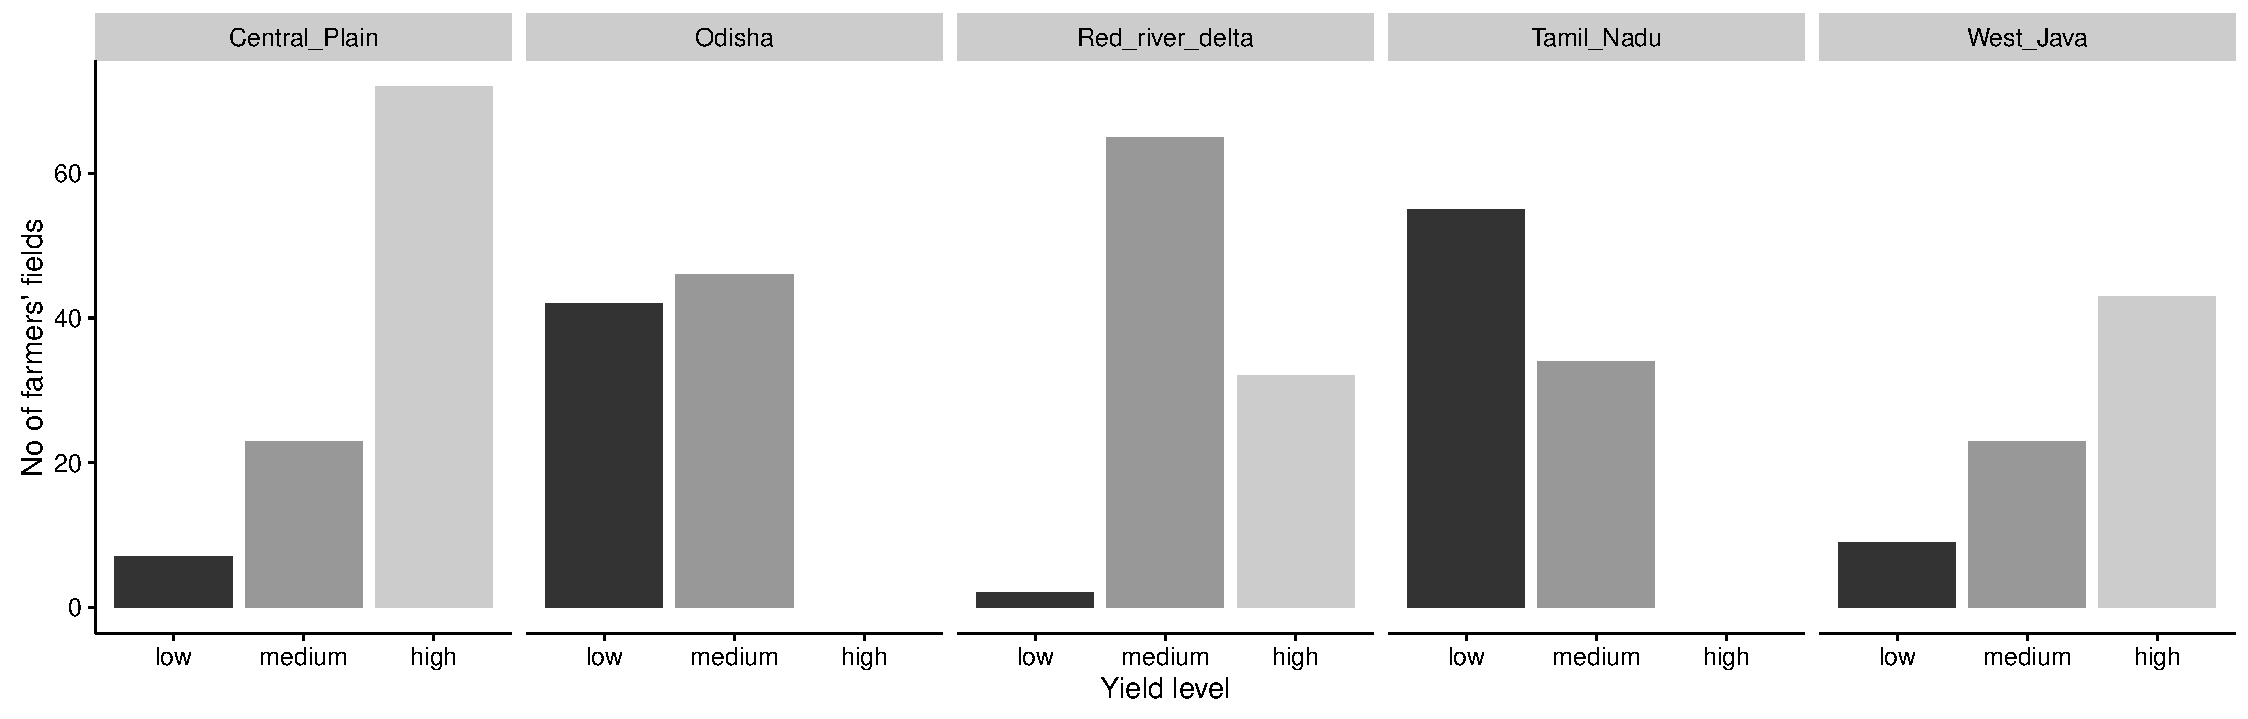
\includegraphics[width = 1\textwidth]{figures/yield_level_bar.pdf}
\caption{Bar graphs showing number of farmers' fields classified by different yield levels in each production environment.}
\label{fig:yield_level_bar}
\end{figure}

\begin{figure}
    \centering
    \begin{subfigure}[b]{1\textwidth}
        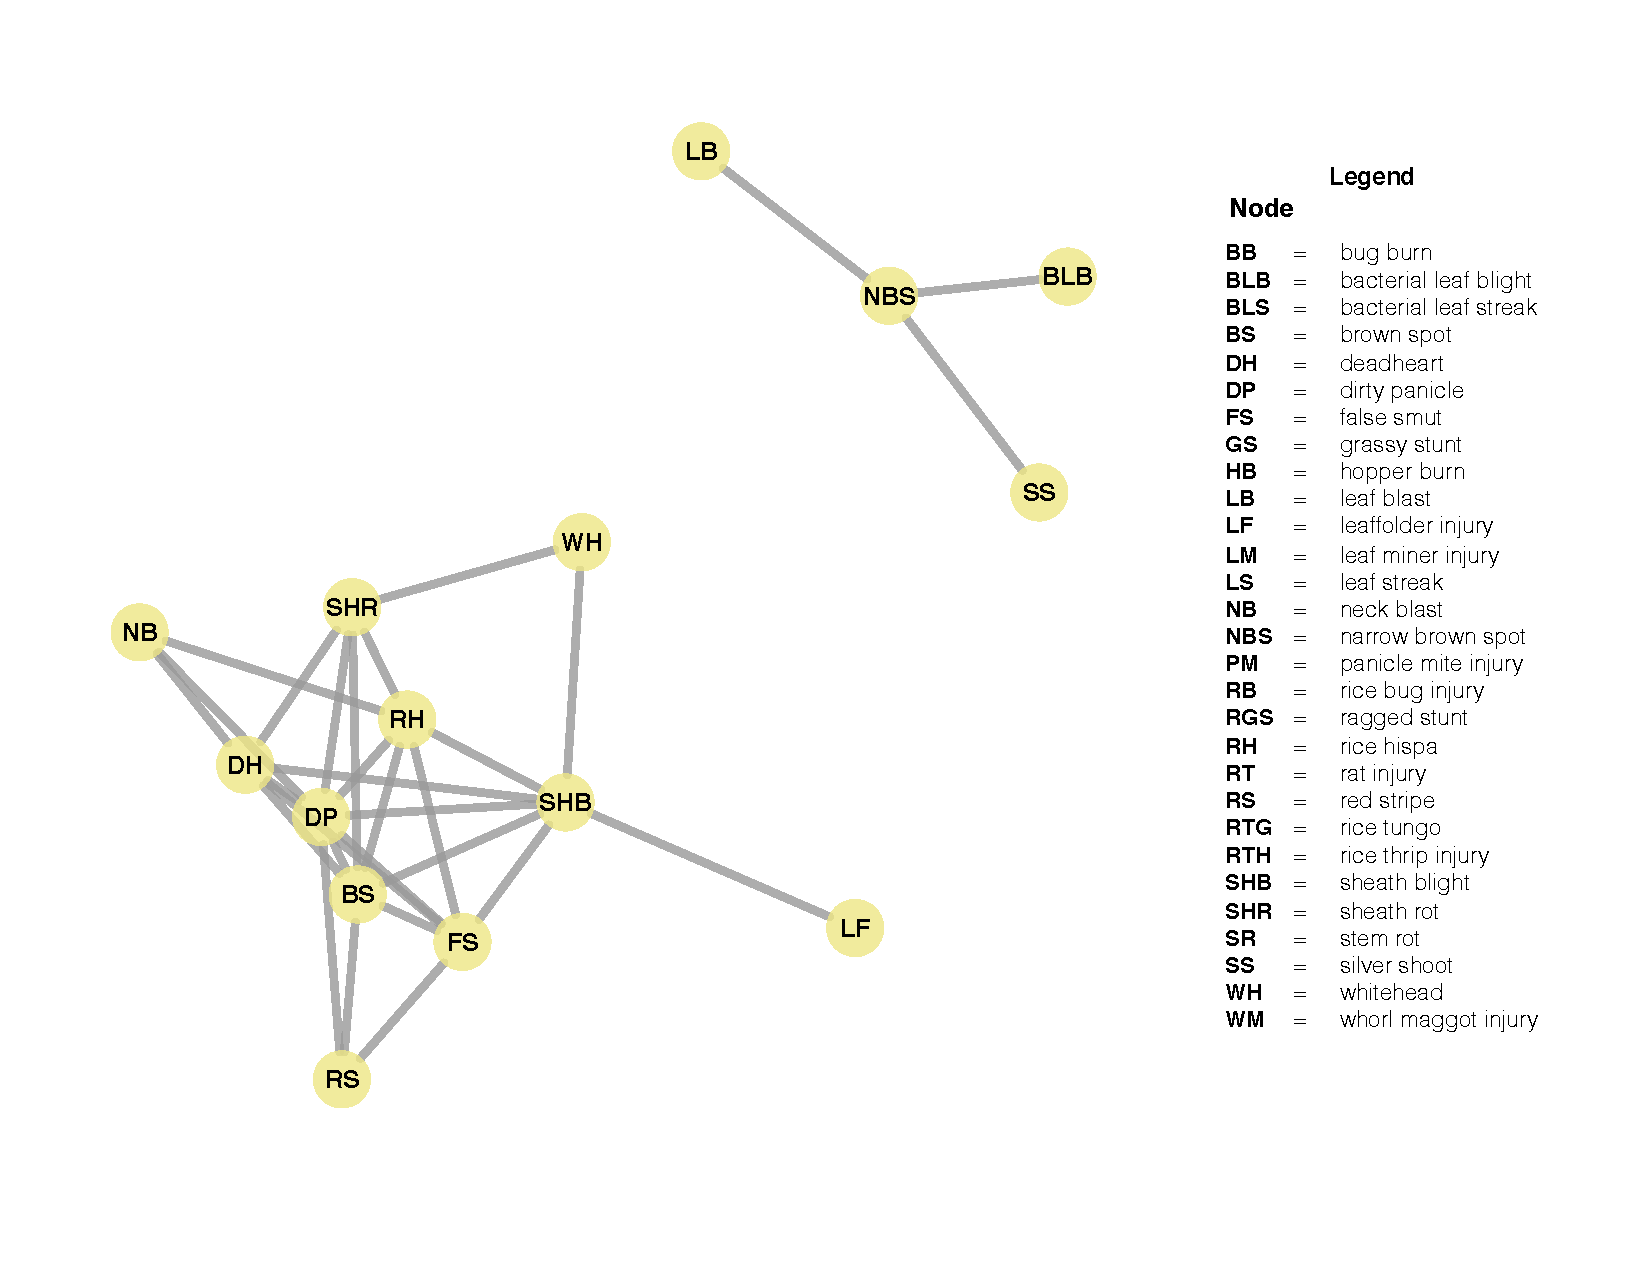
\includegraphics[width = 0.9\textwidth]{figures/difyieldCP.pdf}
        \caption[Differential co-occurrence network of rice injuries in different yield levels at Central Plain, Thailand]{Differential co-occurrence network of rice injuries in different yield levels at Central Plain, Thailand. The layout of the network graph is based on the Fruchterman-Reingold algorithm, which places nodes with stronger or more connections closer to each other.}
        \label{fig:difyieldnetwork_CP}
    \end{subfigure}
    \begin{subfigure}[b]{0.9\textwidth}
        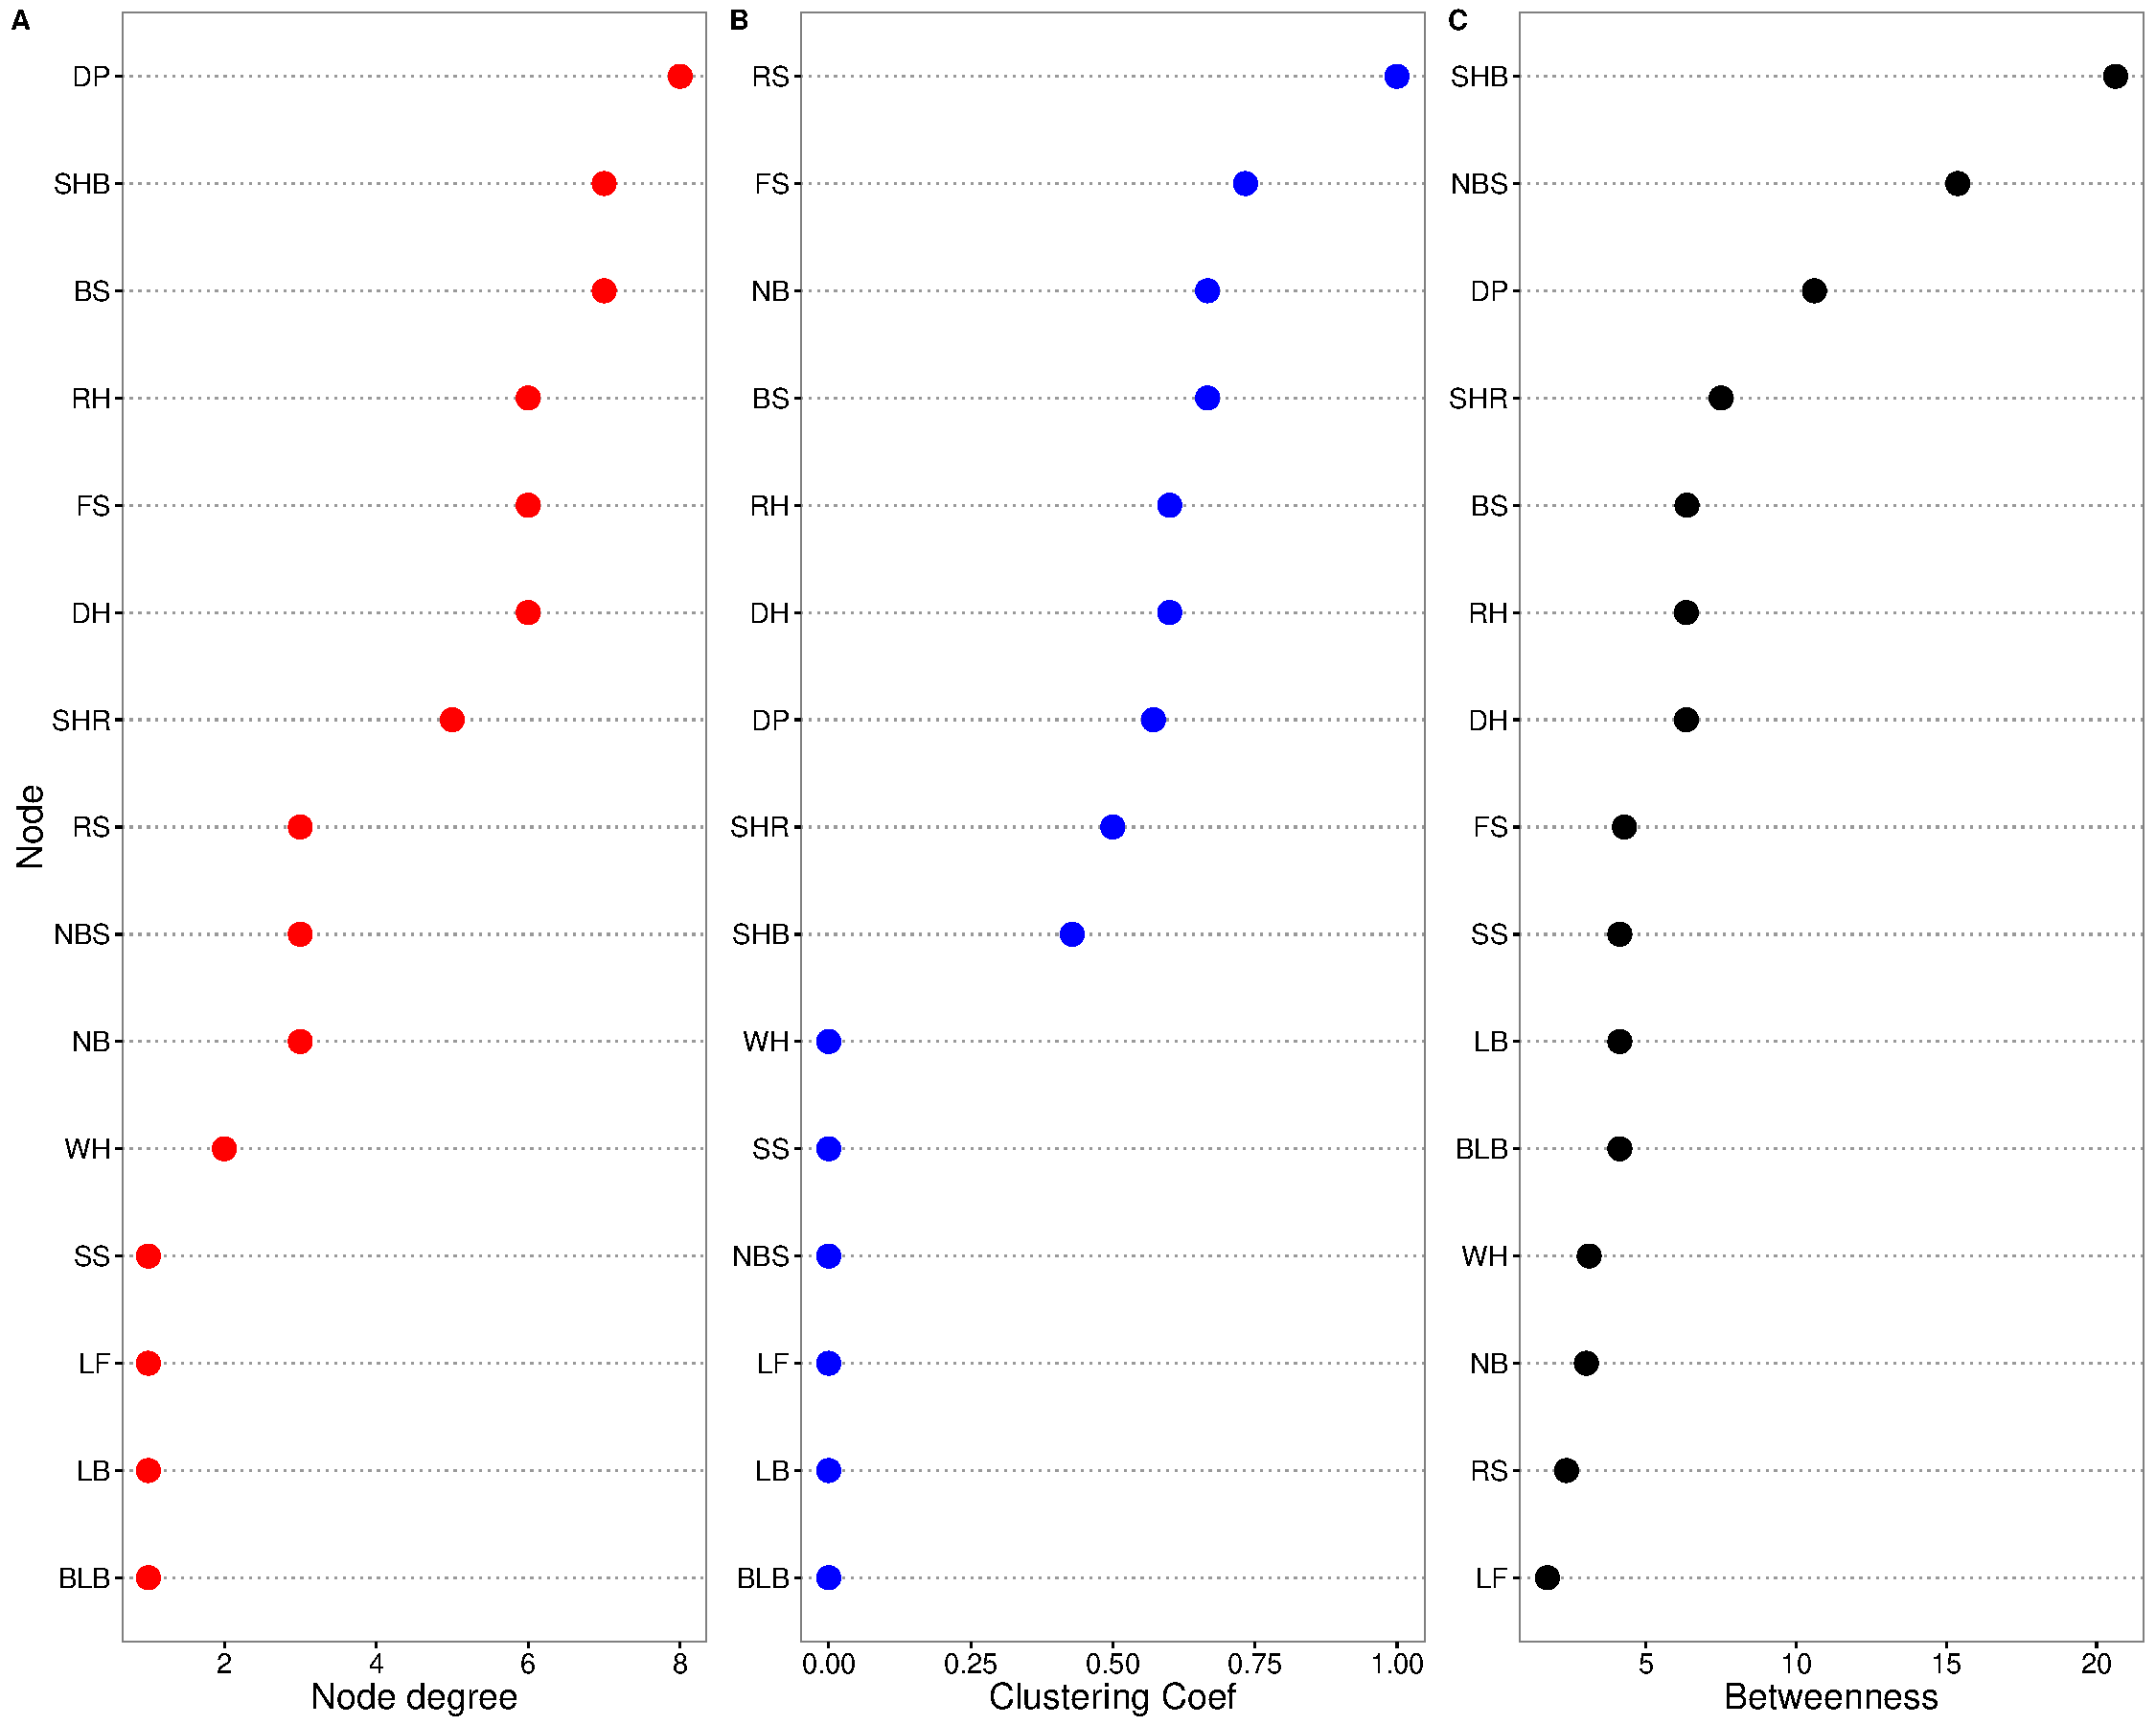
\includegraphics[width = 1\textwidth]{figures/yield_dif_nodepropCentral_Plain.pdf}
        \caption[Three centrality measures of the nodes in co-occurrence network of rice injuries in dry season at Central Plain.]{Three centrality measures of the nodes in co-occurrence network of rice injuries in dry season at Central Plain. A: node degree, B:clustering coefficient, and C:Betweenness.}
        \label{fig:nodepropdifyield_CP}
    \end{subfigure}
    \caption{Differential network analysis of survey data in different yield levels at Central Plain, Thailand.}
    \label{fig:difyield_CP}
\end{figure}
 
\begin{figure}
    \centering
    \begin{subfigure}[b]{1\textwidth}
        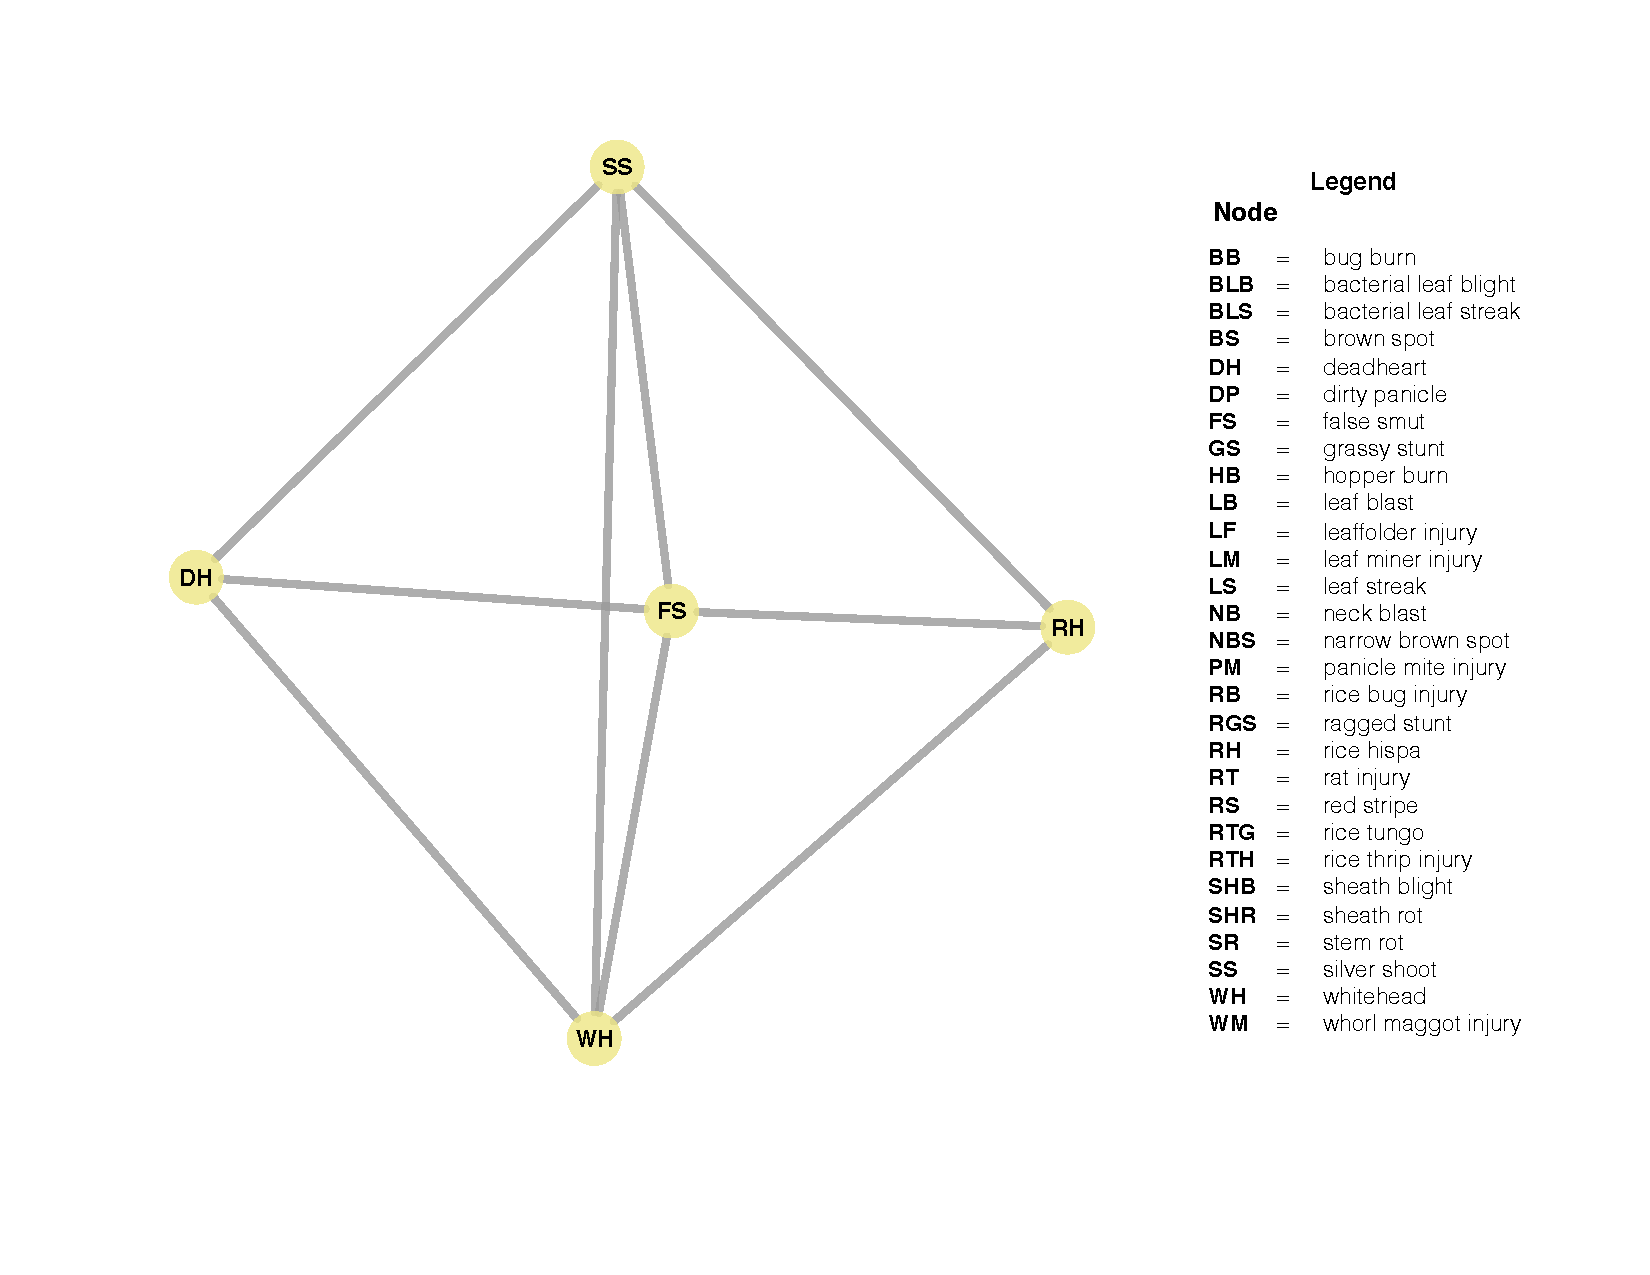
\includegraphics[width = 1\textwidth]{figures/difyieldOD.pdf}
        \caption[Differential co-occurrence network of rice injuries in different yield levels at Odisha, India.]{Differential co-occurrence network of rice injuries in different yield levels at Odisha, India. The layout of the network graph is based on the Fruchterman-Reingold algorithm, which places nodes with stronger or more connections closer to each other.}
        \label{fig:difyieldnetwork_OD}
    \end{subfigure}
    \begin{subfigure}[b]{1\textwidth}
        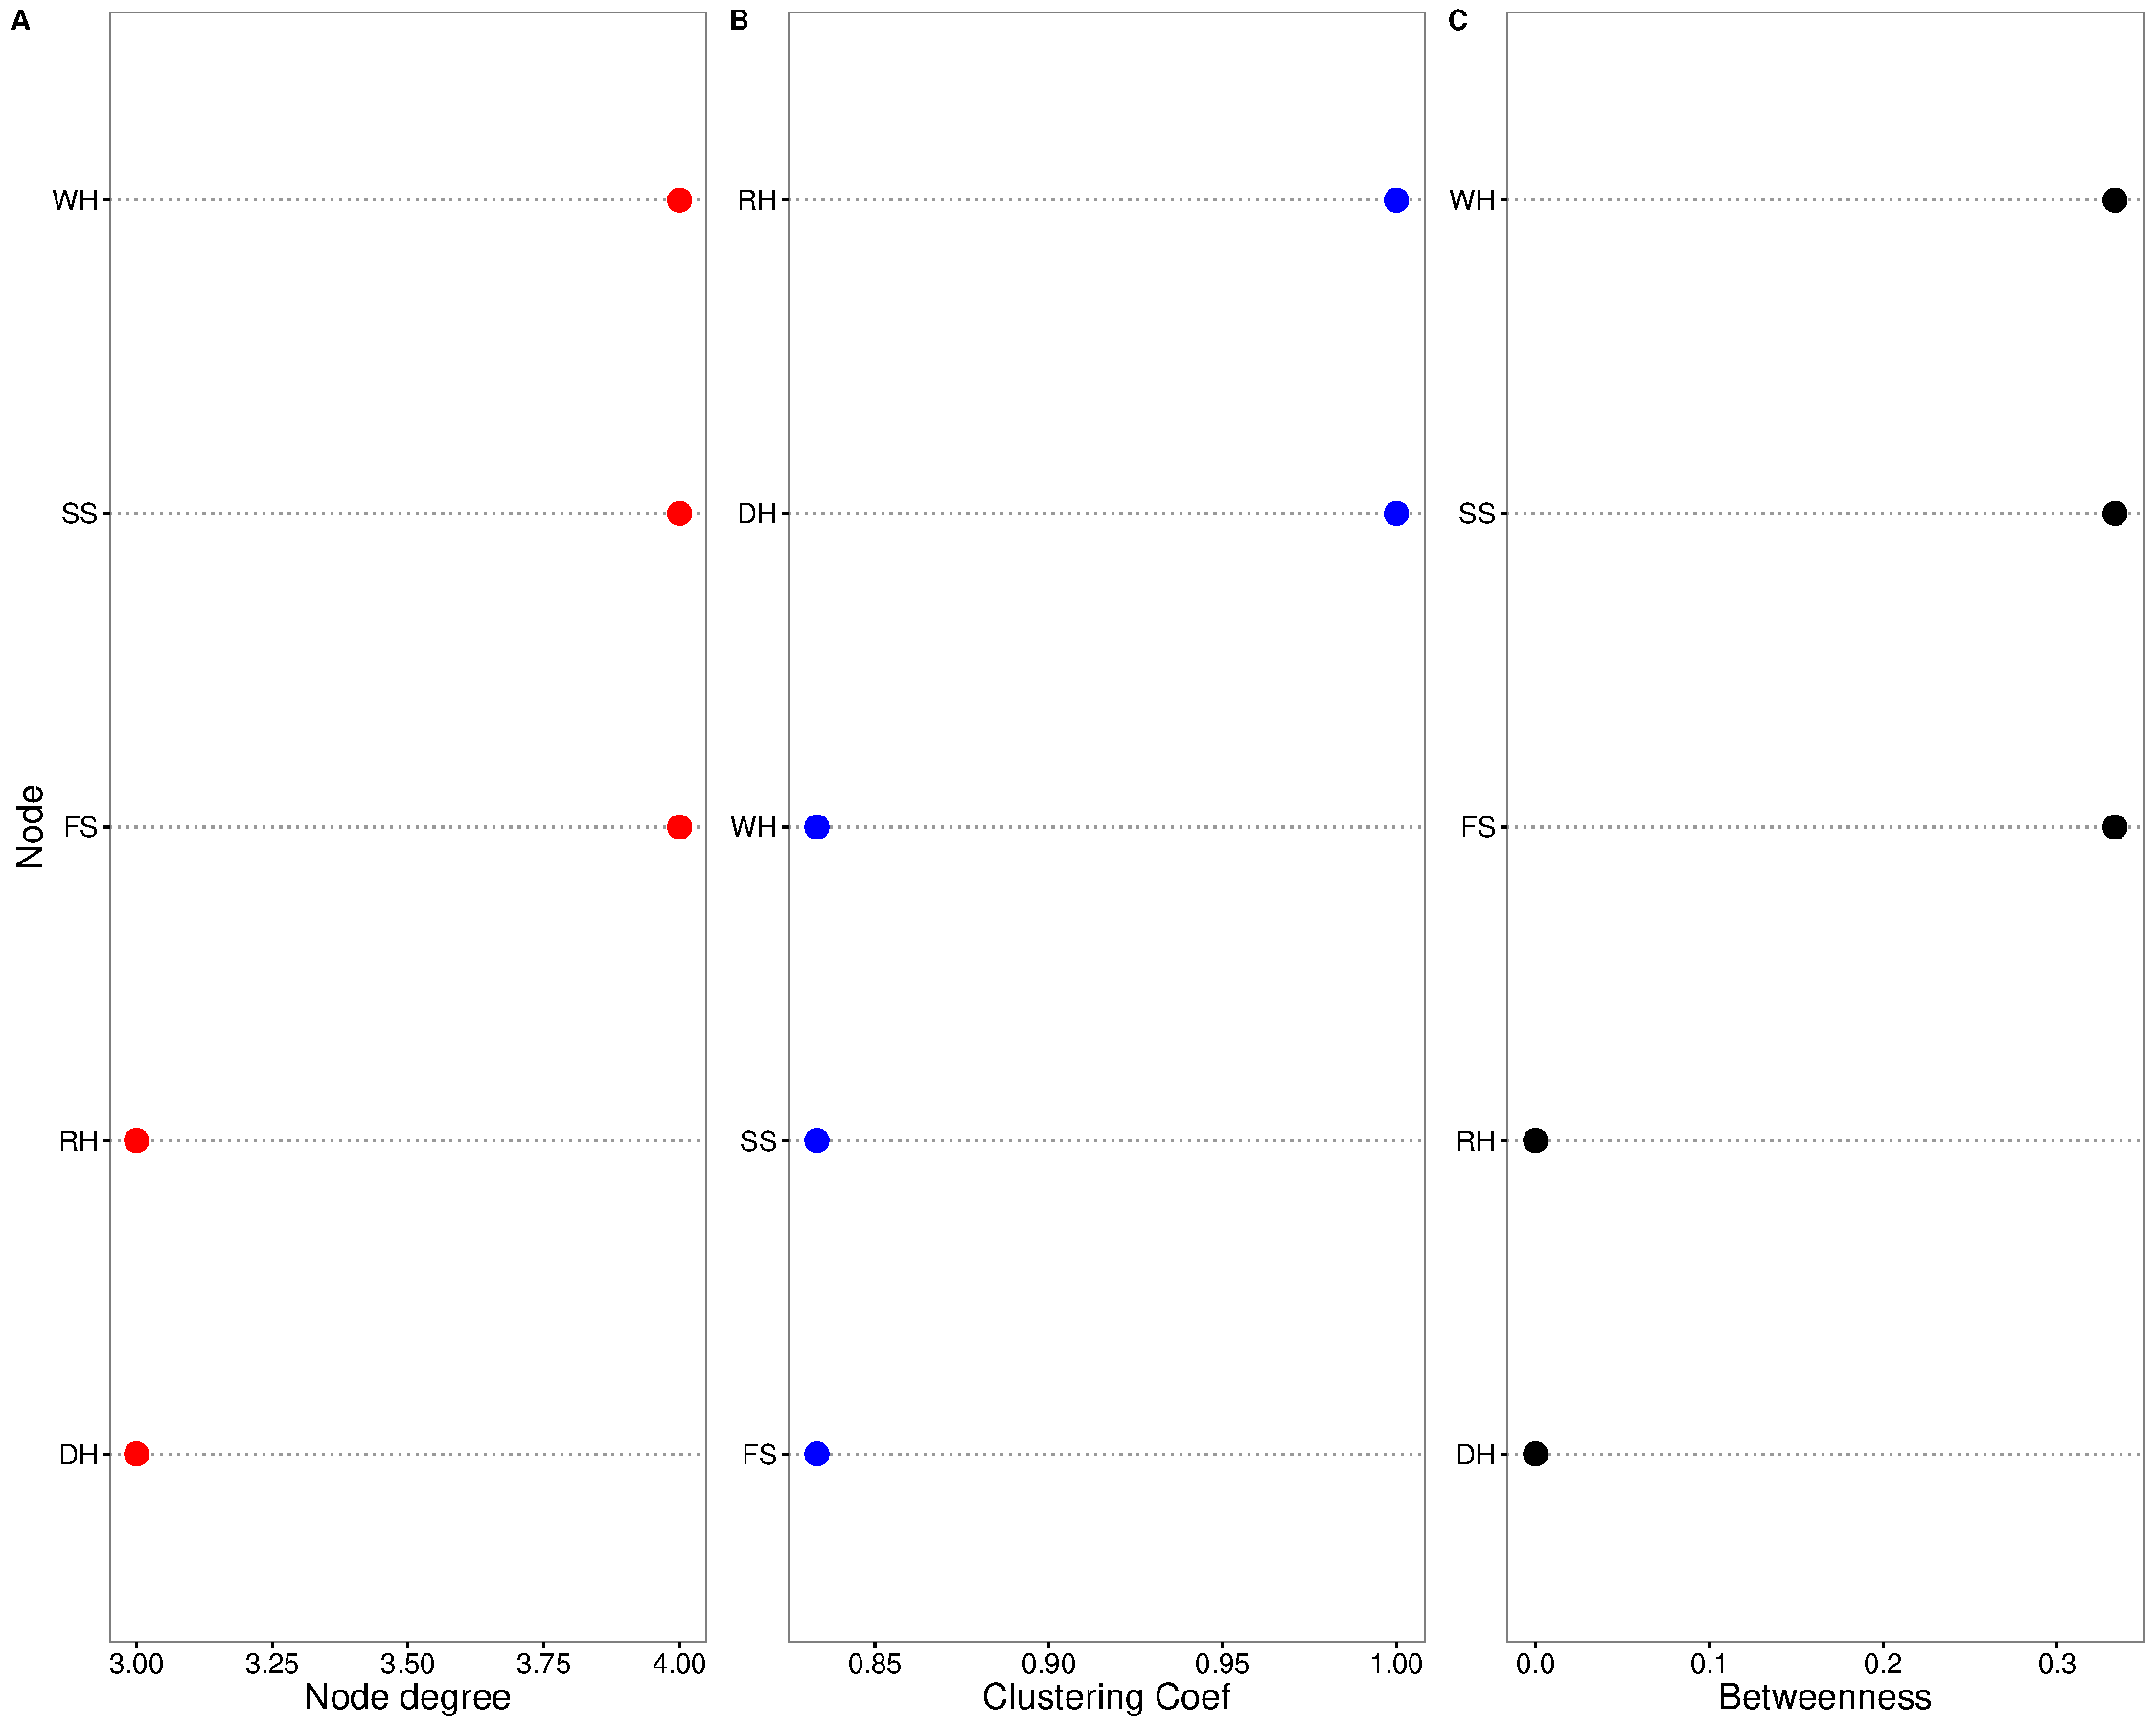
\includegraphics[width = 1\textwidth]{figures/yield_dif_nodepropOdisha.pdf}
        \caption[Three centrality measures of the nodes in co-occurrence network of rice injuries in dry season at Odisha, India.]{Three centrality measures of the nodes in co-occurrence network of rice injuries in dry season at Odisha, India. A: node degree, B:clustering coefficient, and C:Betweenness.}
        \label{fig:nodepropdifyield_OD}
    \end{subfigure}
    \caption{Differential network analysis of survey data in different yield levels at Odisha, India.}
    \label{fig:difyield_OD}
\end{figure}
 
 \begin{figure}
    \centering
    \begin{subfigure}[b]{1\textwidth}
        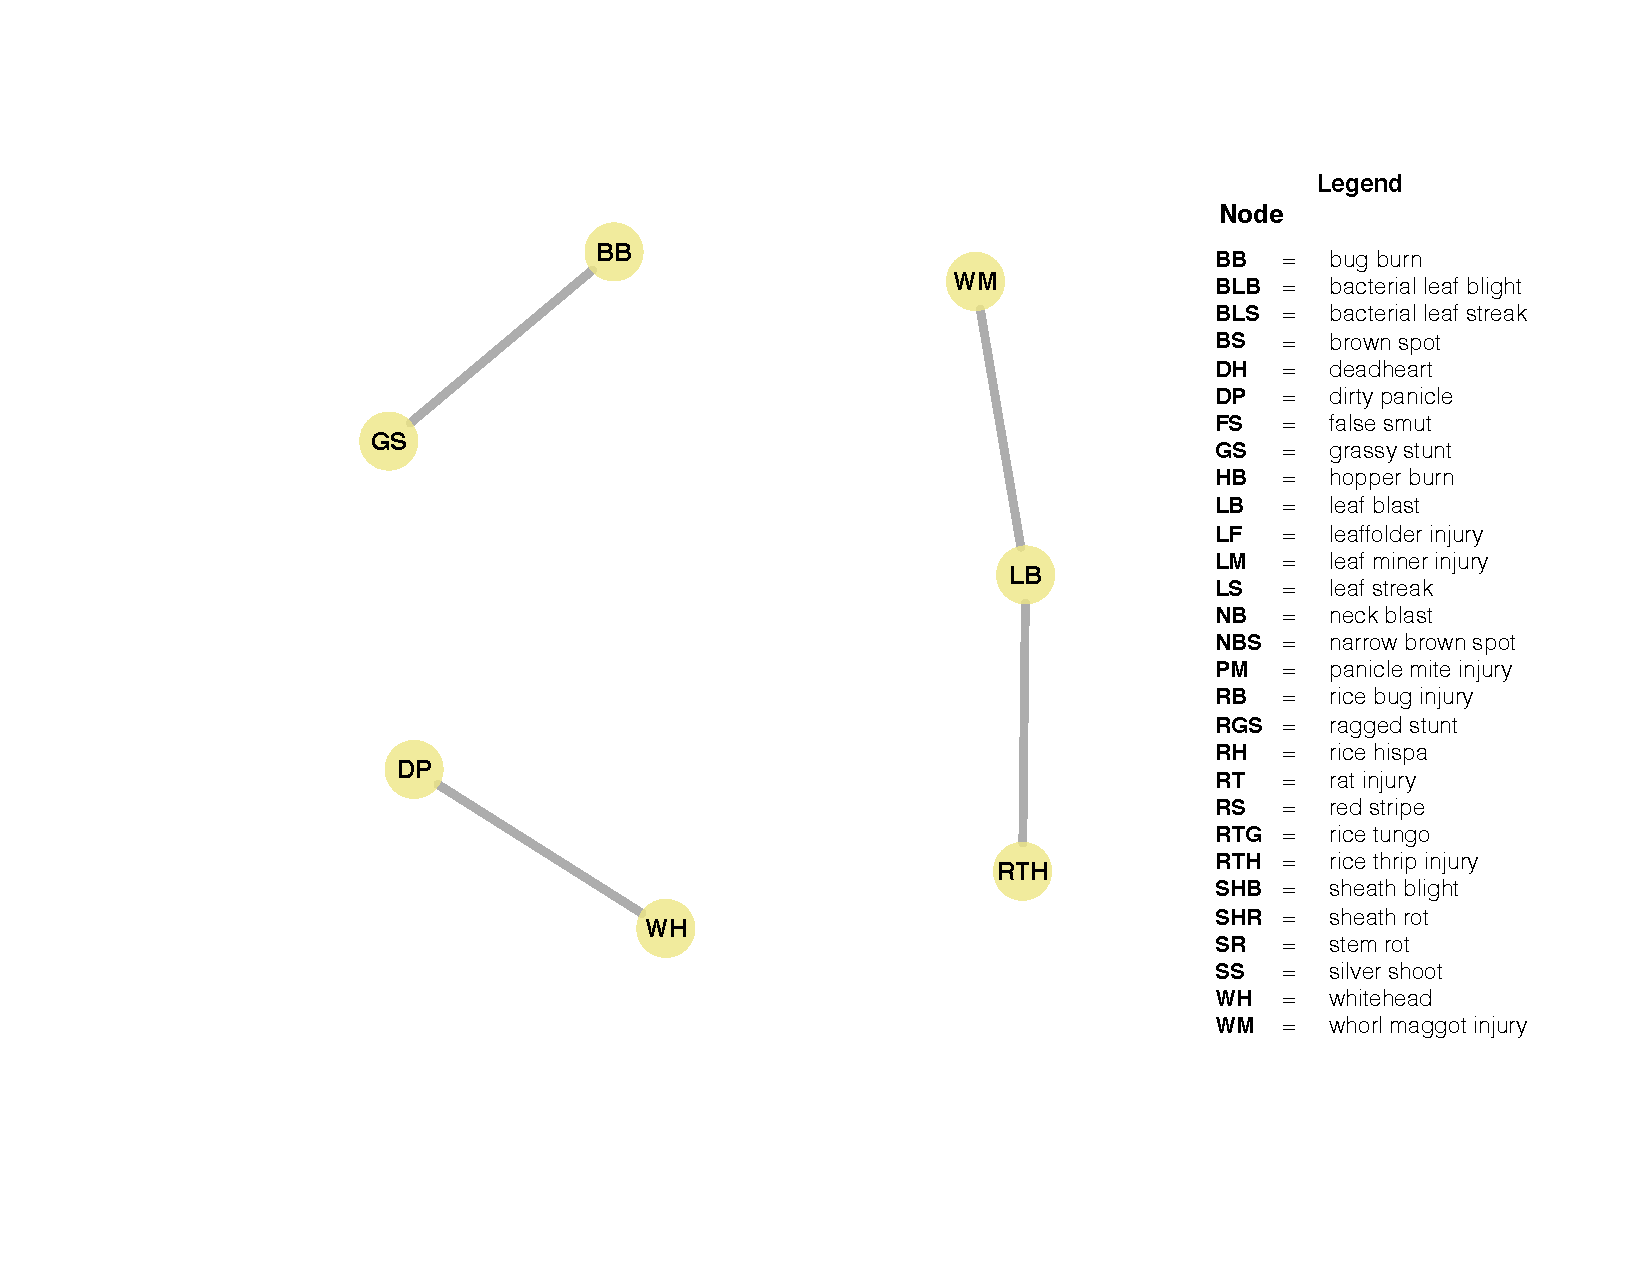
\includegraphics[width = 1\textwidth]{figures/difyieldRR.pdf}
        \caption[Differential co-occurrence network of rice injuries in different yield levels at Red River Delta, Vietnam. ]{Differential co-occurrence network of rice injuries in different yield levels at Red River Delta, Vietnam. The layout of the network graph is based on the Fruchterman-Reingold algorithm, which places nodes with stronger or more connections closer to each other.}
        \label{fig:difyieldnetwork_RR}
    \end{subfigure}
    \begin{subfigure}[b]{1\textwidth}
        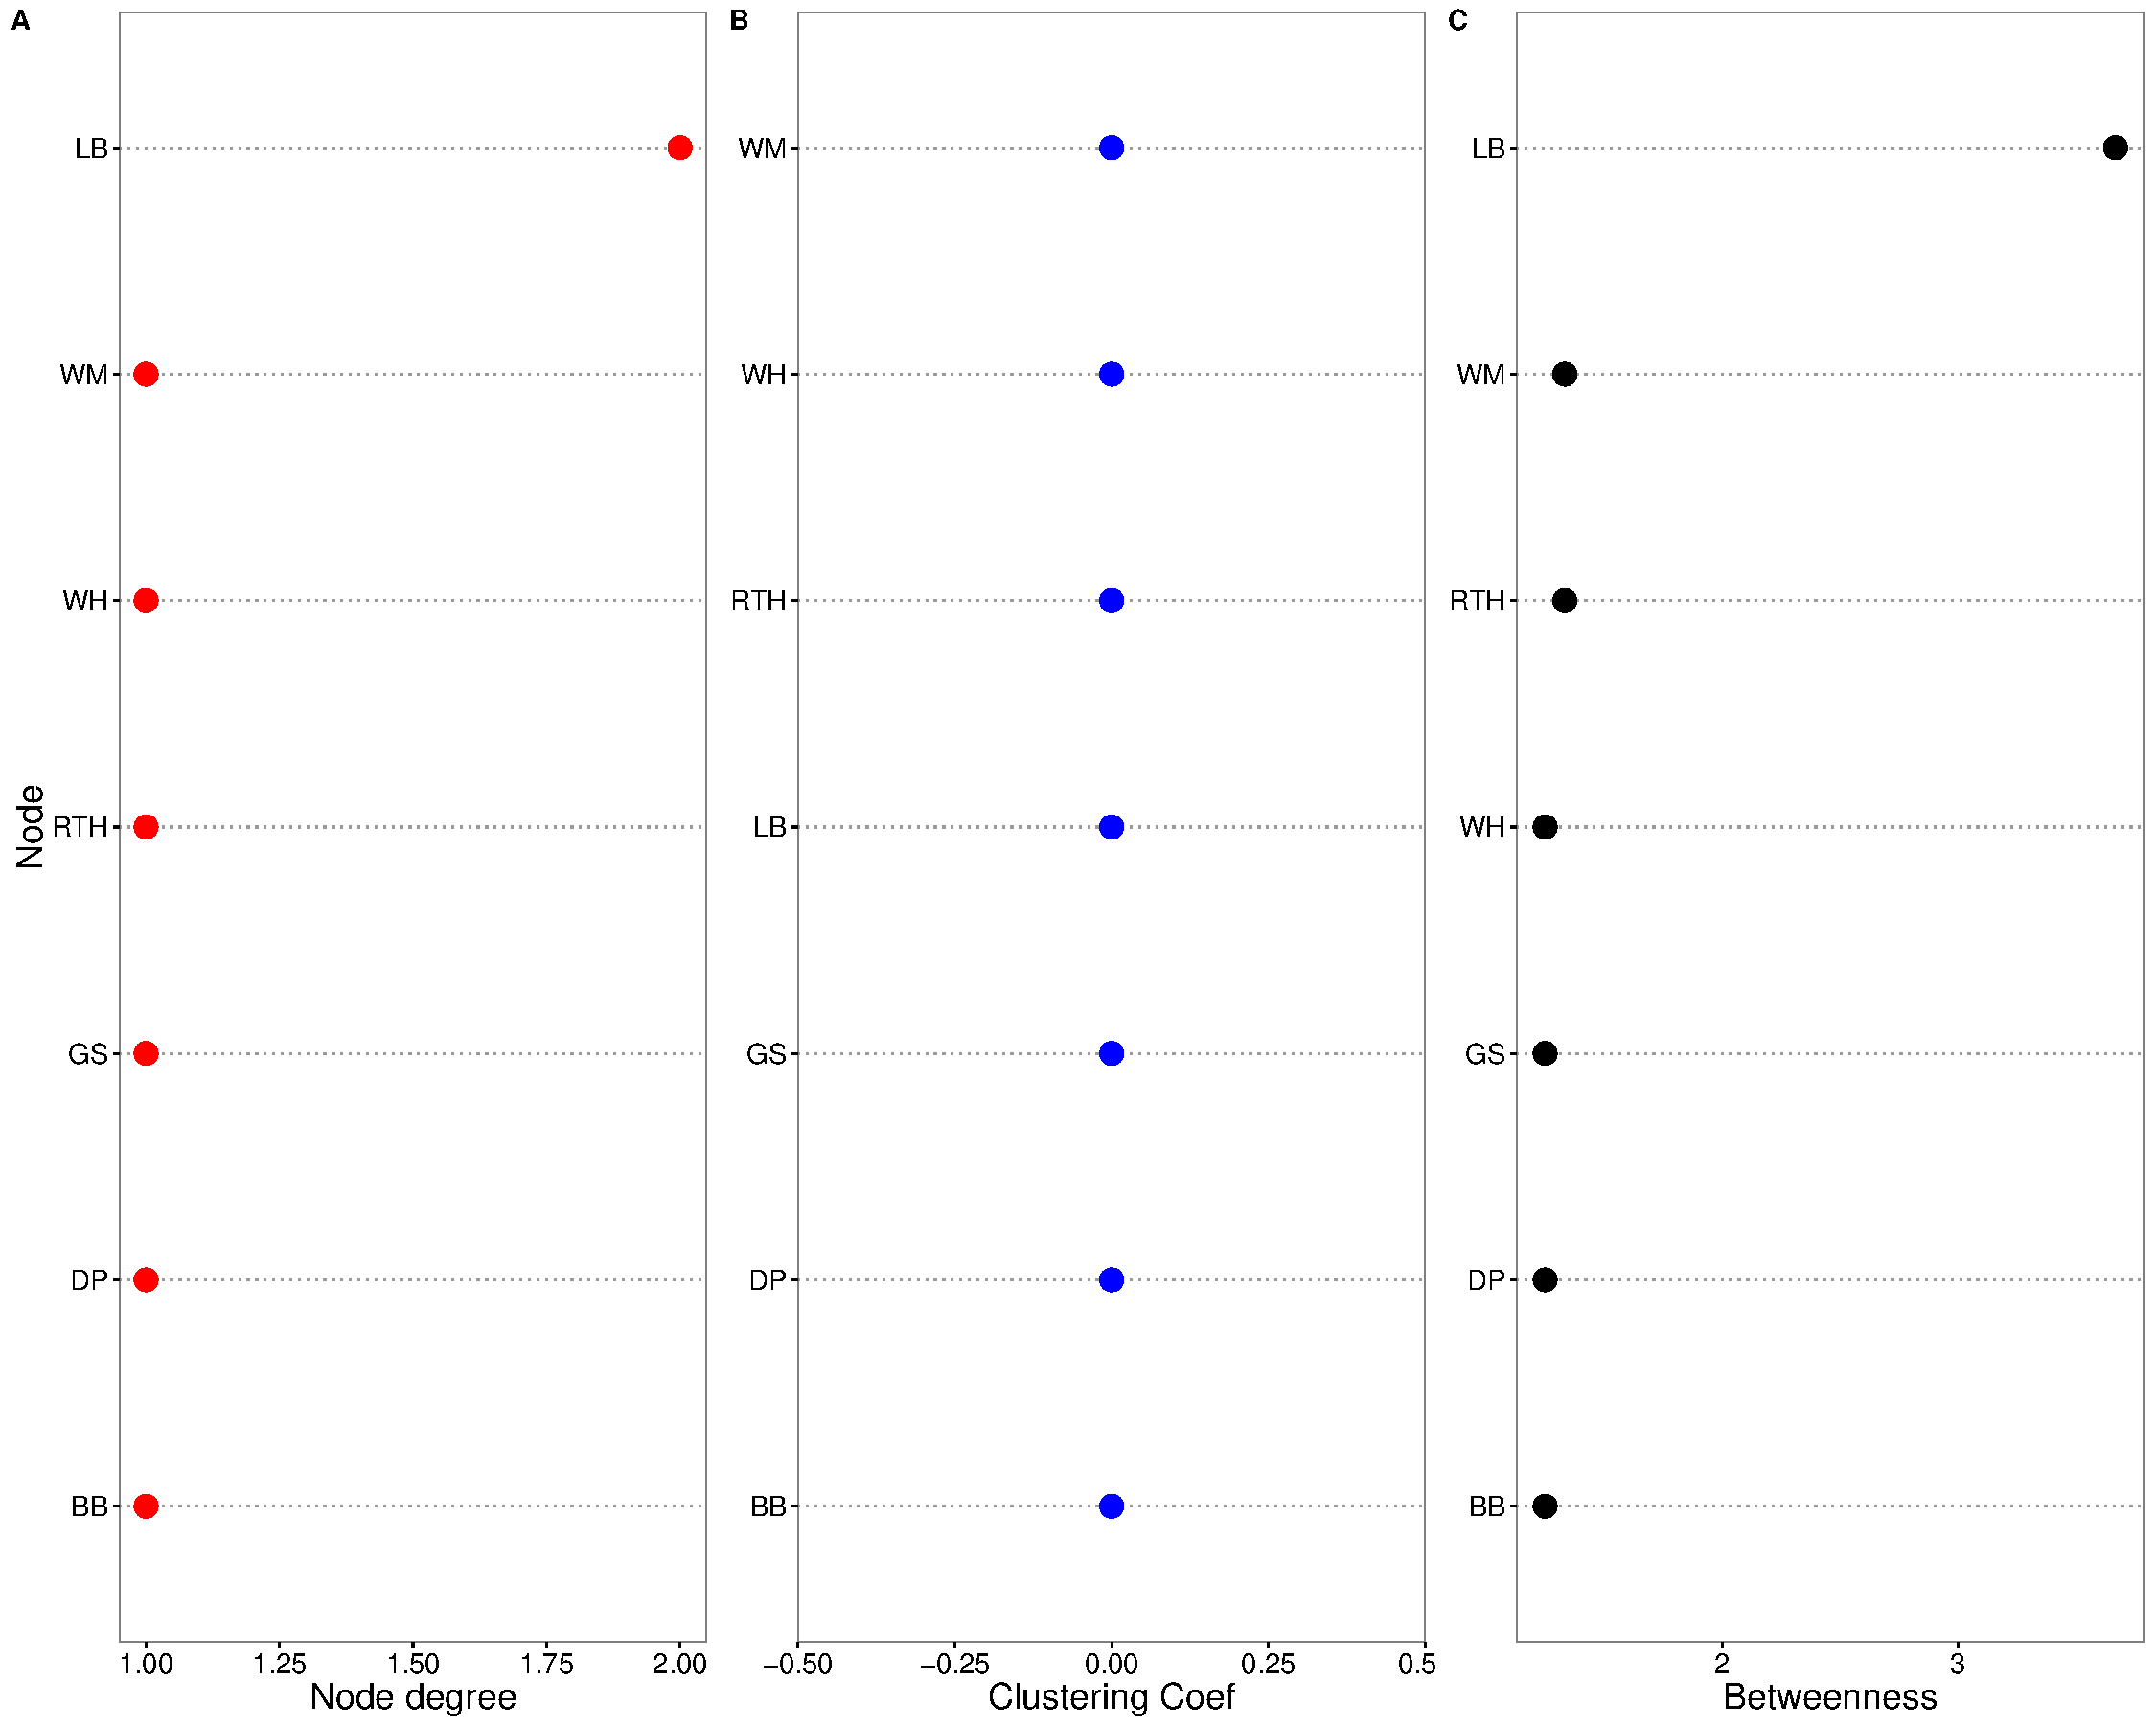
\includegraphics[width = 1\textwidth]{figures/yield_dif_nodepropRed_River_Delta.pdf}
        \caption[Three centrality measures of the nodes in differential co-occurrence network of rice injuries in different yield levels at Red River Delta, Vietnam]{Three centrality measures of the nodes in differential co-occurrence network of rice injuries in different yield levels at Red River Delta, Vietnam. A: node degree, B:clustering coefficient, and C:Betweenness.}
        \label{fig:nodepropdifyield_RR}
    \end{subfigure}
    \caption{Differential network analysis of survey data in different yield levels at Red River Delta, Vietnam}
    \label{fig:difyield_RR}
\end{figure}
 
 \begin{figure}
    \centering
    \begin{subfigure}[b]{1\textwidth}
        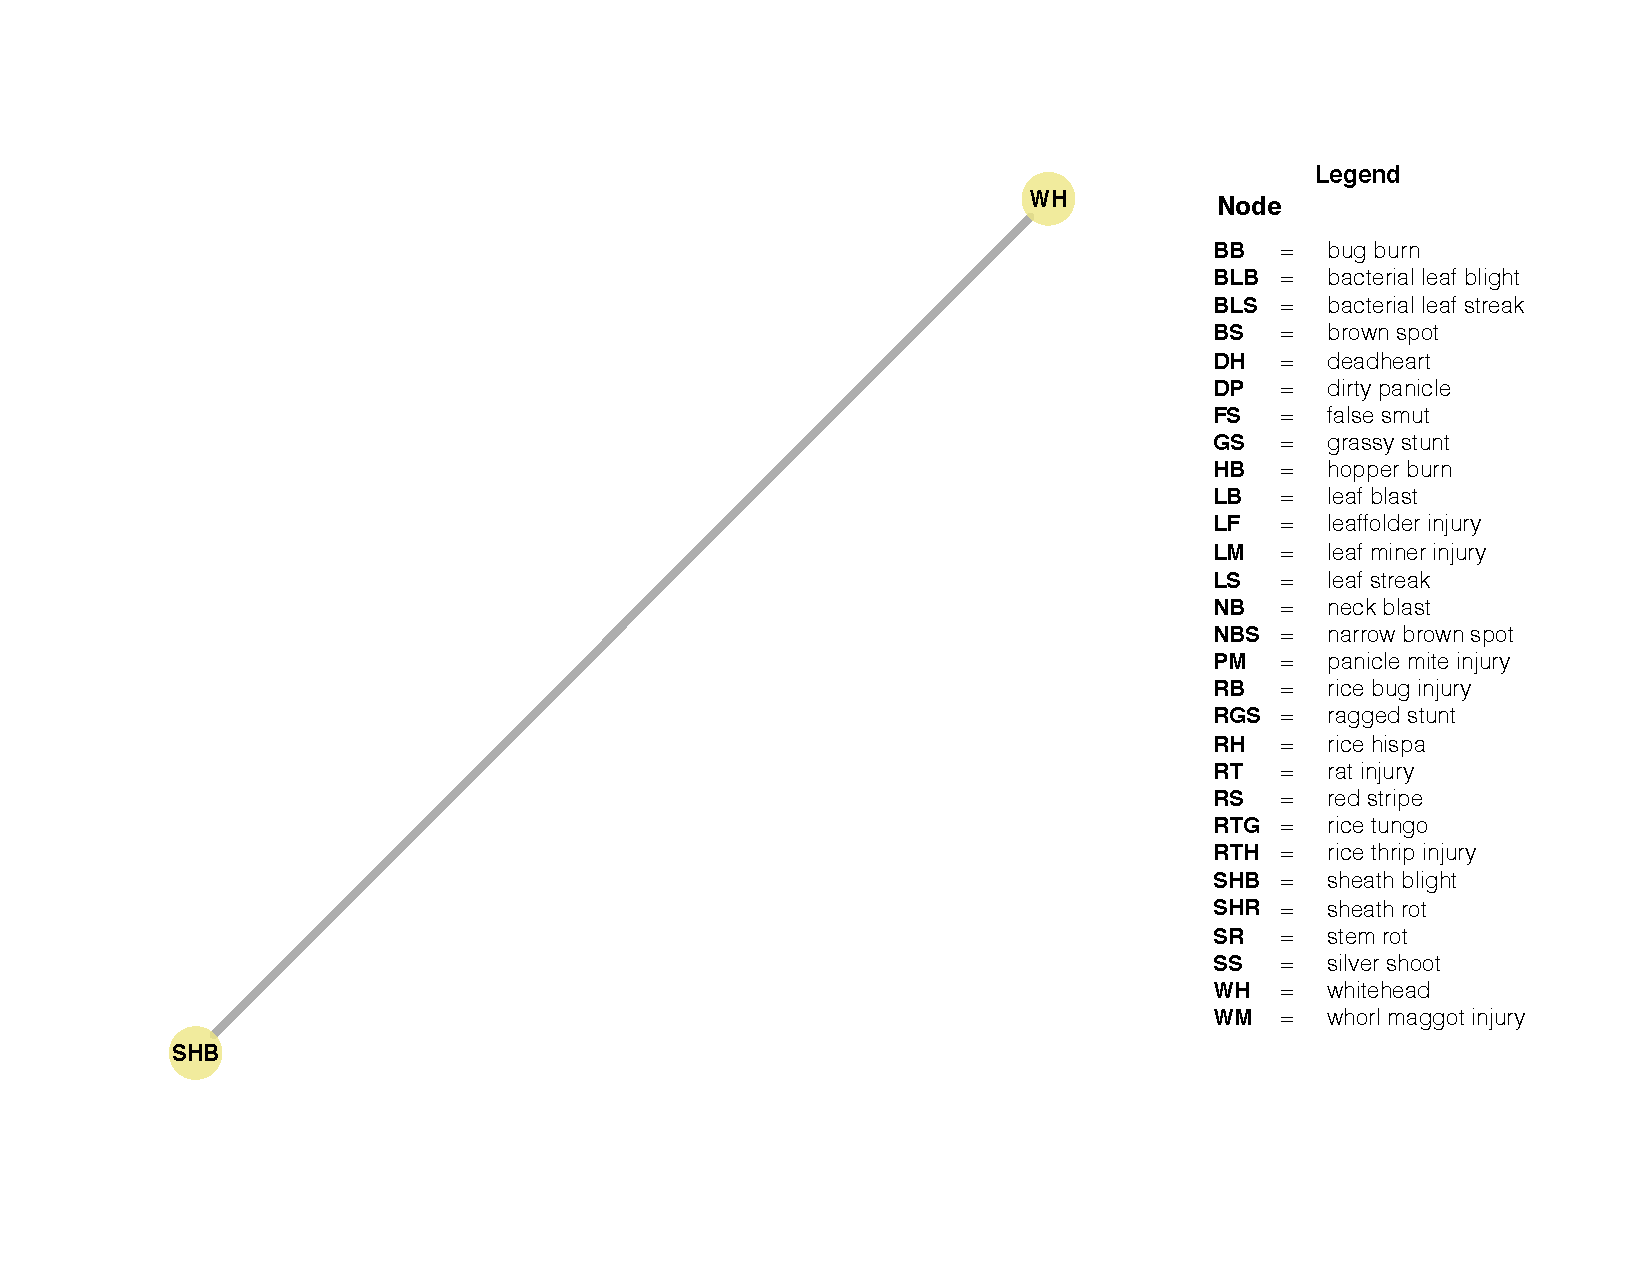
\includegraphics[width = 1\textwidth]{figures/difyieldTM.pdf}
        \caption[Differential co-occurrence network of rice injuries in different yield levels at Tamil Nadu, India.]{Differential co-occurrence network of rice injuries in different yield levels at Tamil Nadu, India. The layout of the network graph is based on the Fruchterman-Reingold algorithm, which places nodes with stronger or more connections closer to each other.}
        \label{fig:difyieldnetwork_TM}
    \end{subfigure}
    \begin{subfigure}[b]{1\textwidth}
        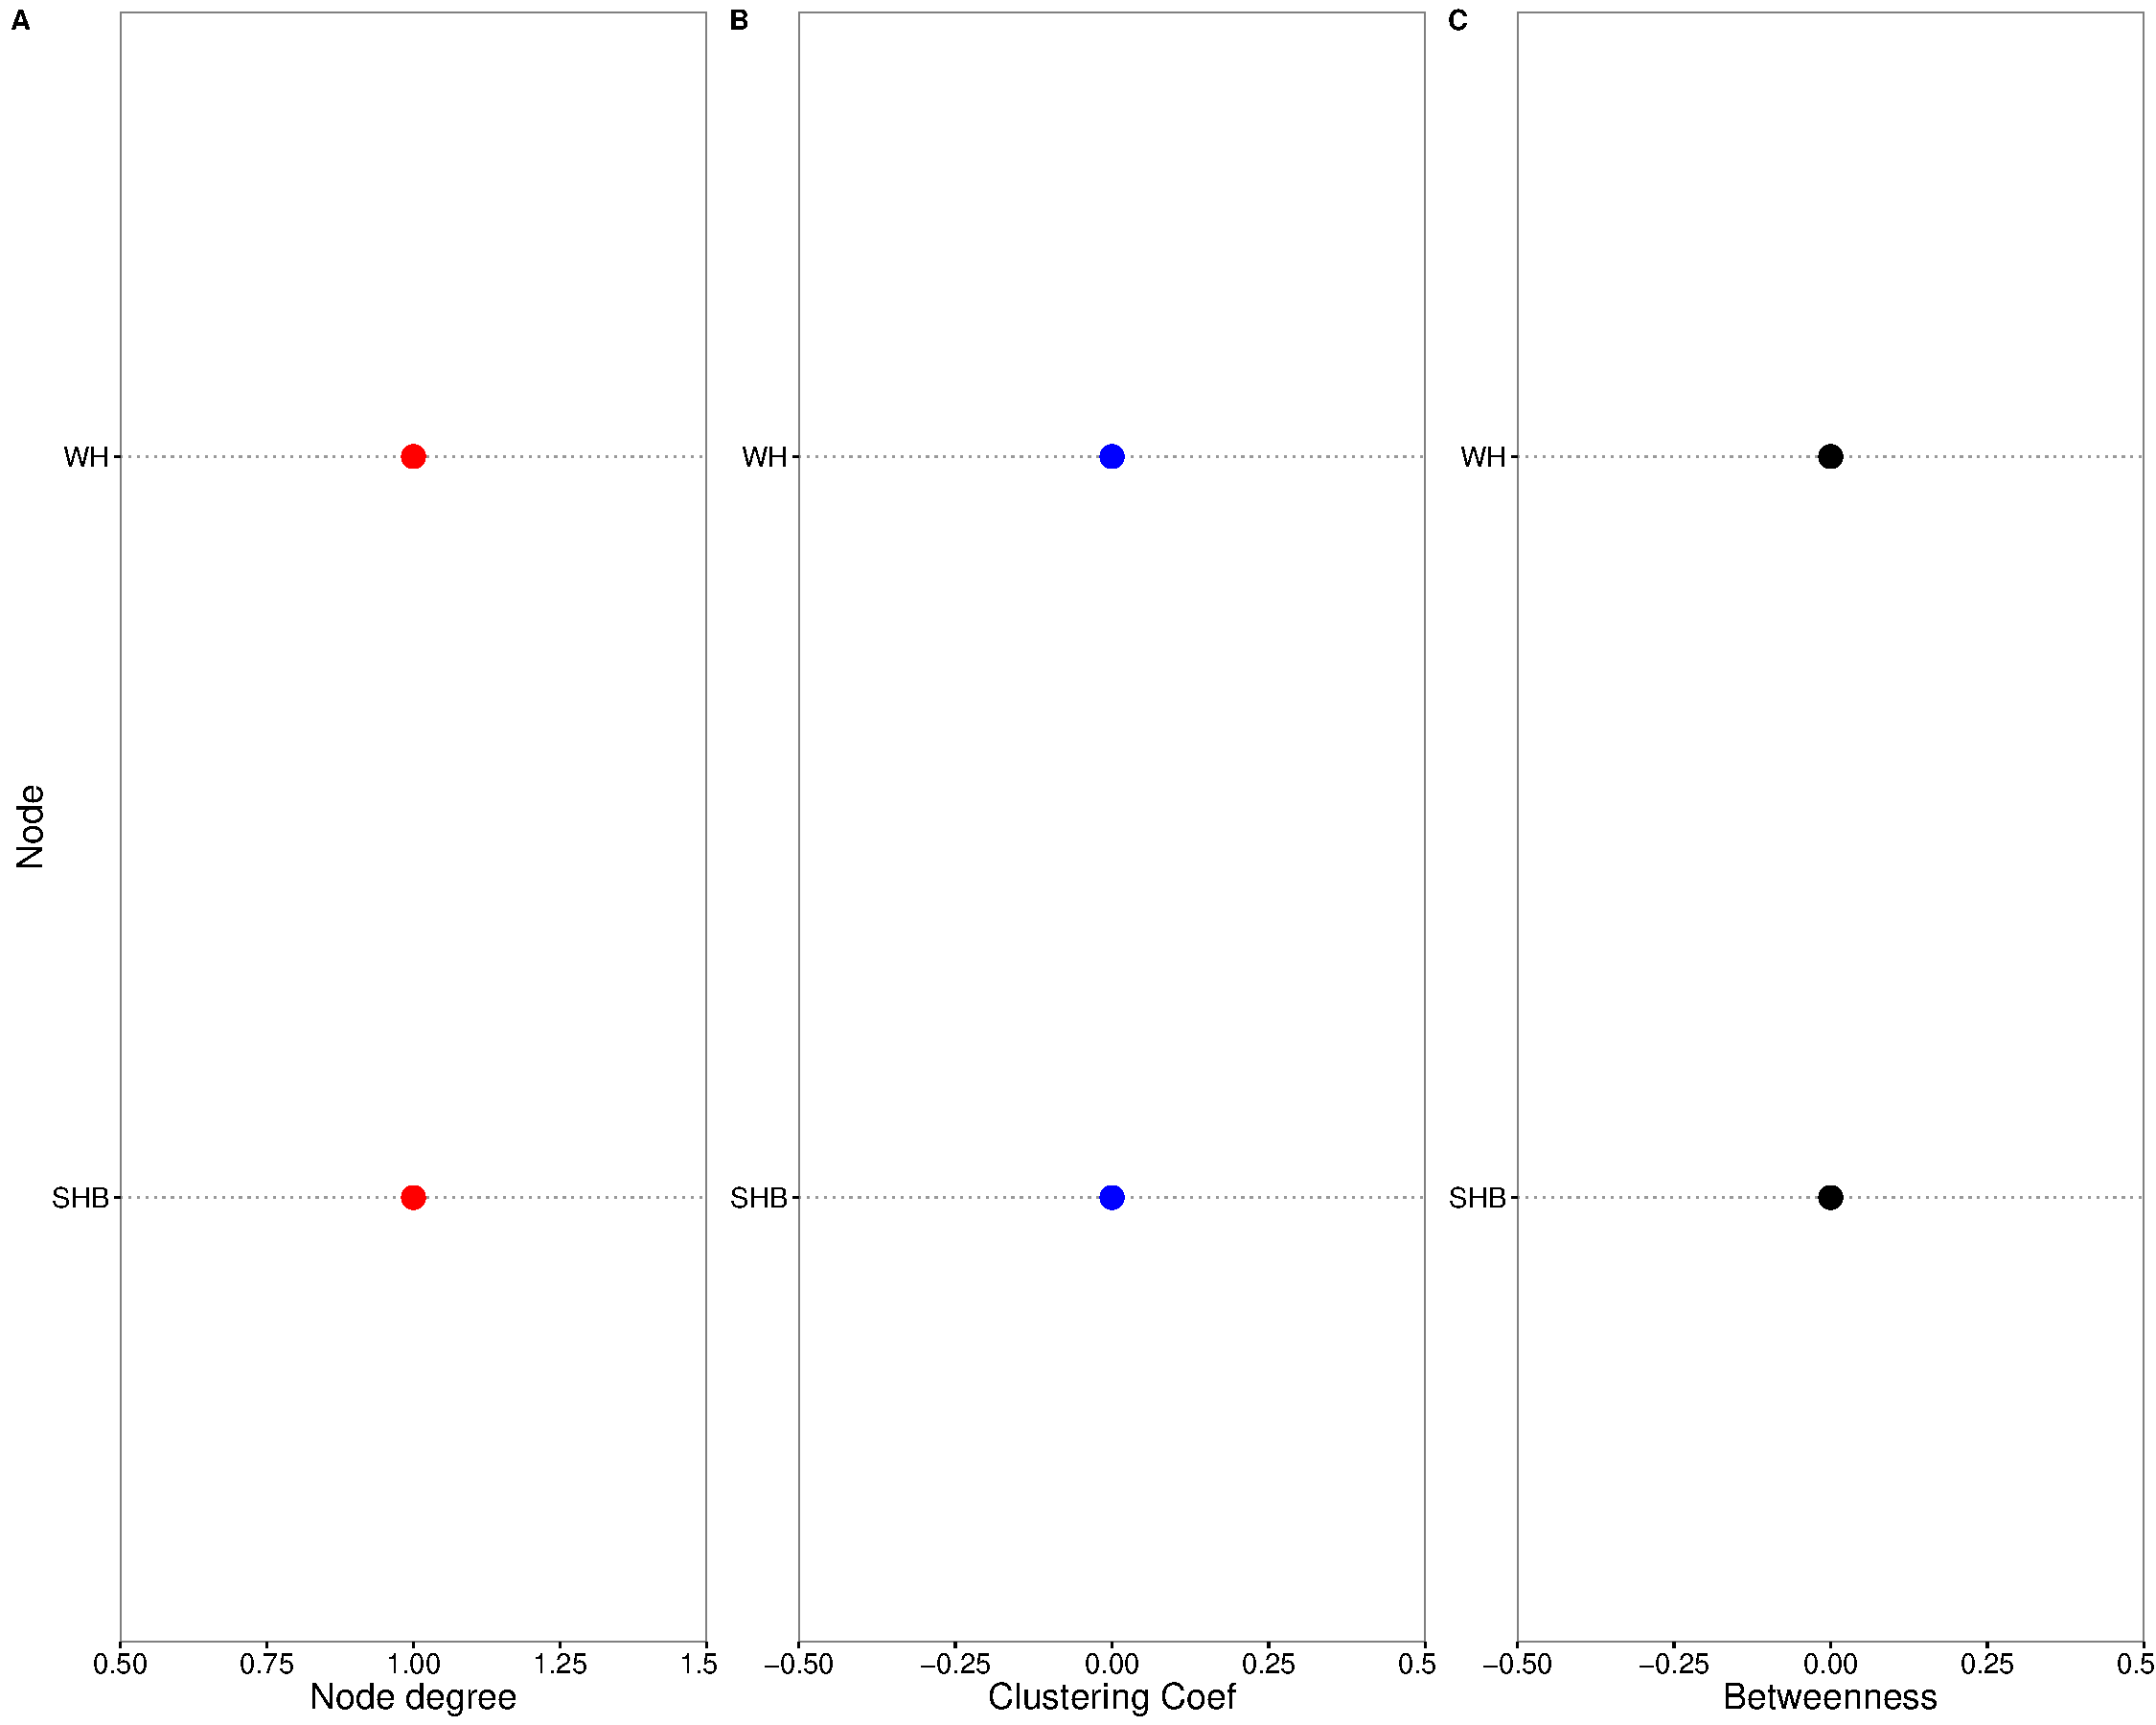
\includegraphics[width = 1\textwidth]{figures/yield_dif_nodepropTamil_Nadu.pdf}
        \caption{Three centrality measures of the nodes in co-occurrence network of rice injuries in dry season at Central Plain. A: node degree, B:clustering coefficient, and C:Betweenness.}
        \label{fig:nodepropdifyield_TM}
    \end{subfigure}
    \caption{Differential network analysis of survey data in different yield levels at Tamil Nadu, India.}
    \label{fig:yielddif_TM}
\end{figure}
 
  
 \begin{figure}
    \centering
    \begin{subfigure}[b]{1\textwidth}
        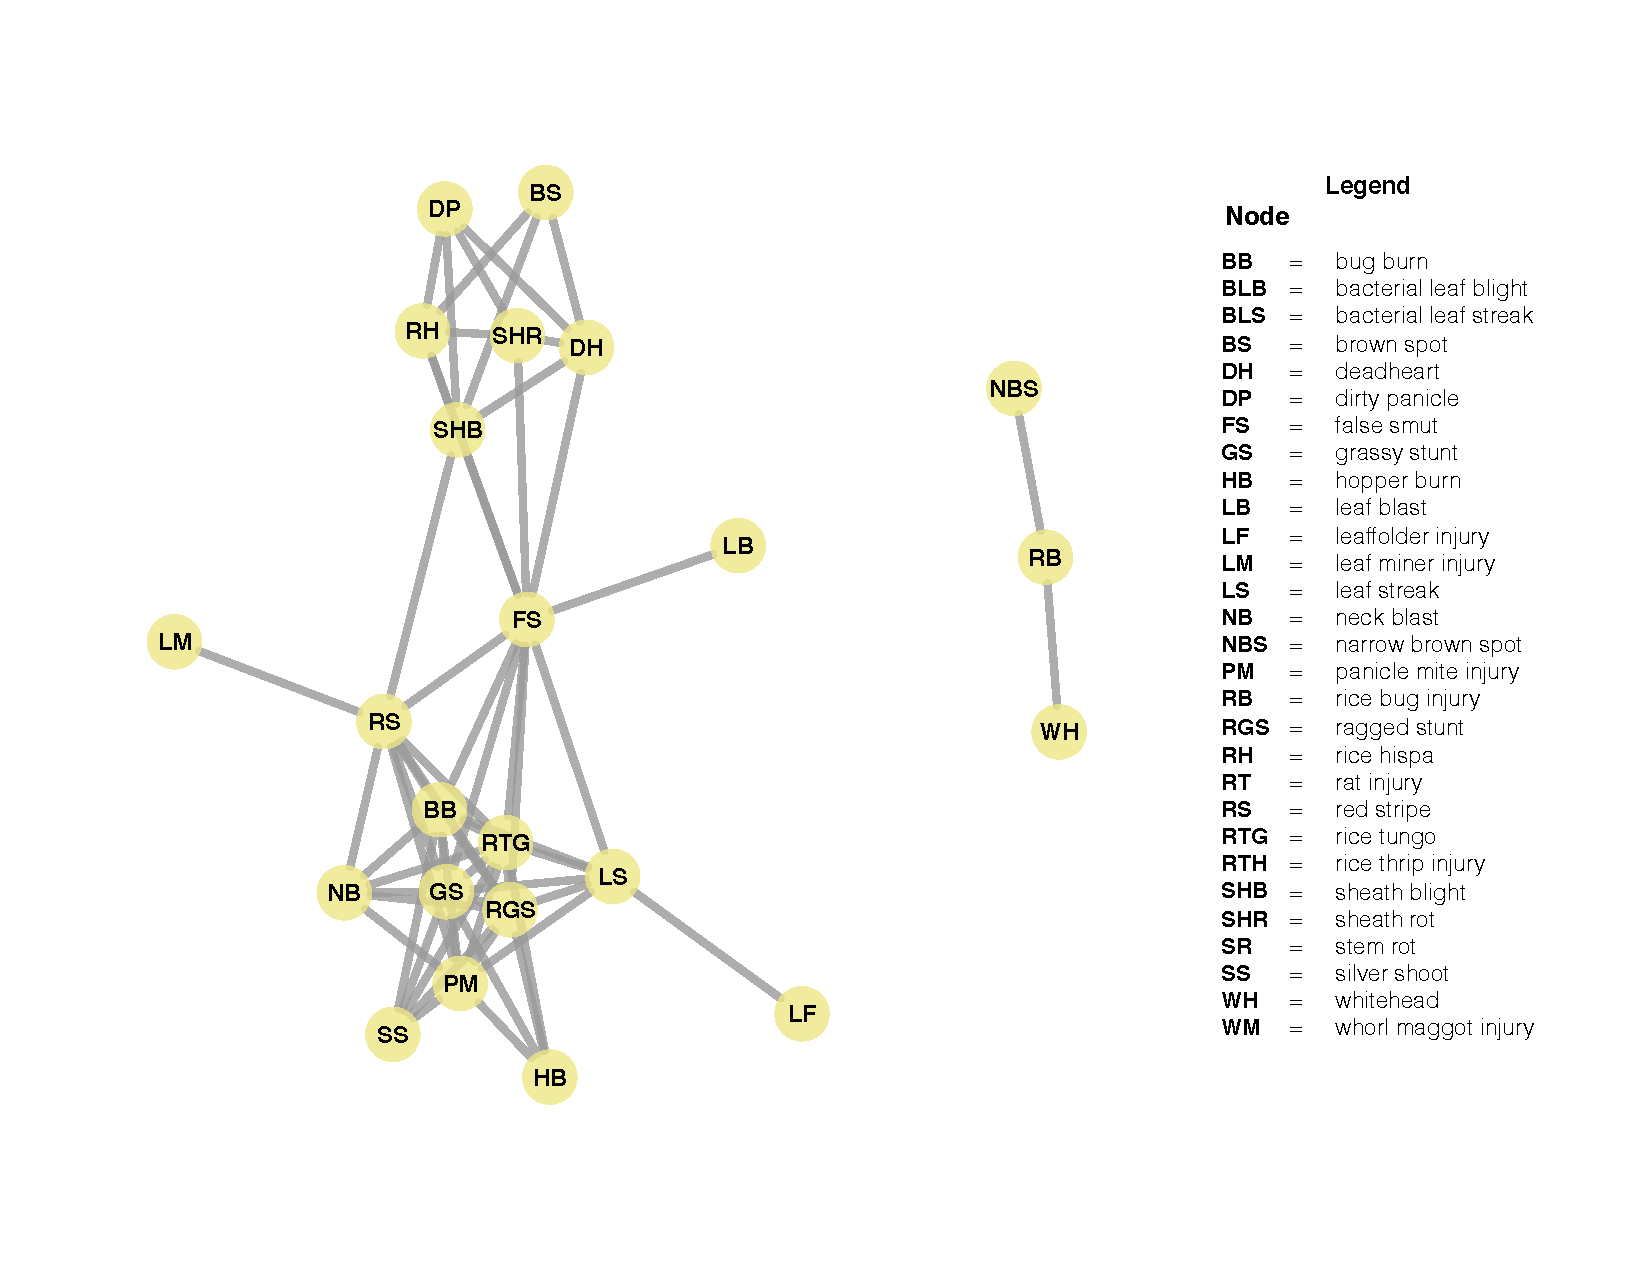
\includegraphics[width = 1\textwidth]{figures/difyieldWJ.pdf}
        \caption[Differential co-occurrence network of rice injuries in different yield levels at West Java, Indonesia.]{Differential co-occurrence network of rice injuries in different yield levels at West Java, Indonesia. The layout of the network graph is based on the Fruchterman-Reingold algorithm, which places nodes with stronger or more connections closer to each other.}
        \label{fig:difyieldnetwork_WJ}
    \end{subfigure}
    \begin{subfigure}[b]{1\textwidth}
        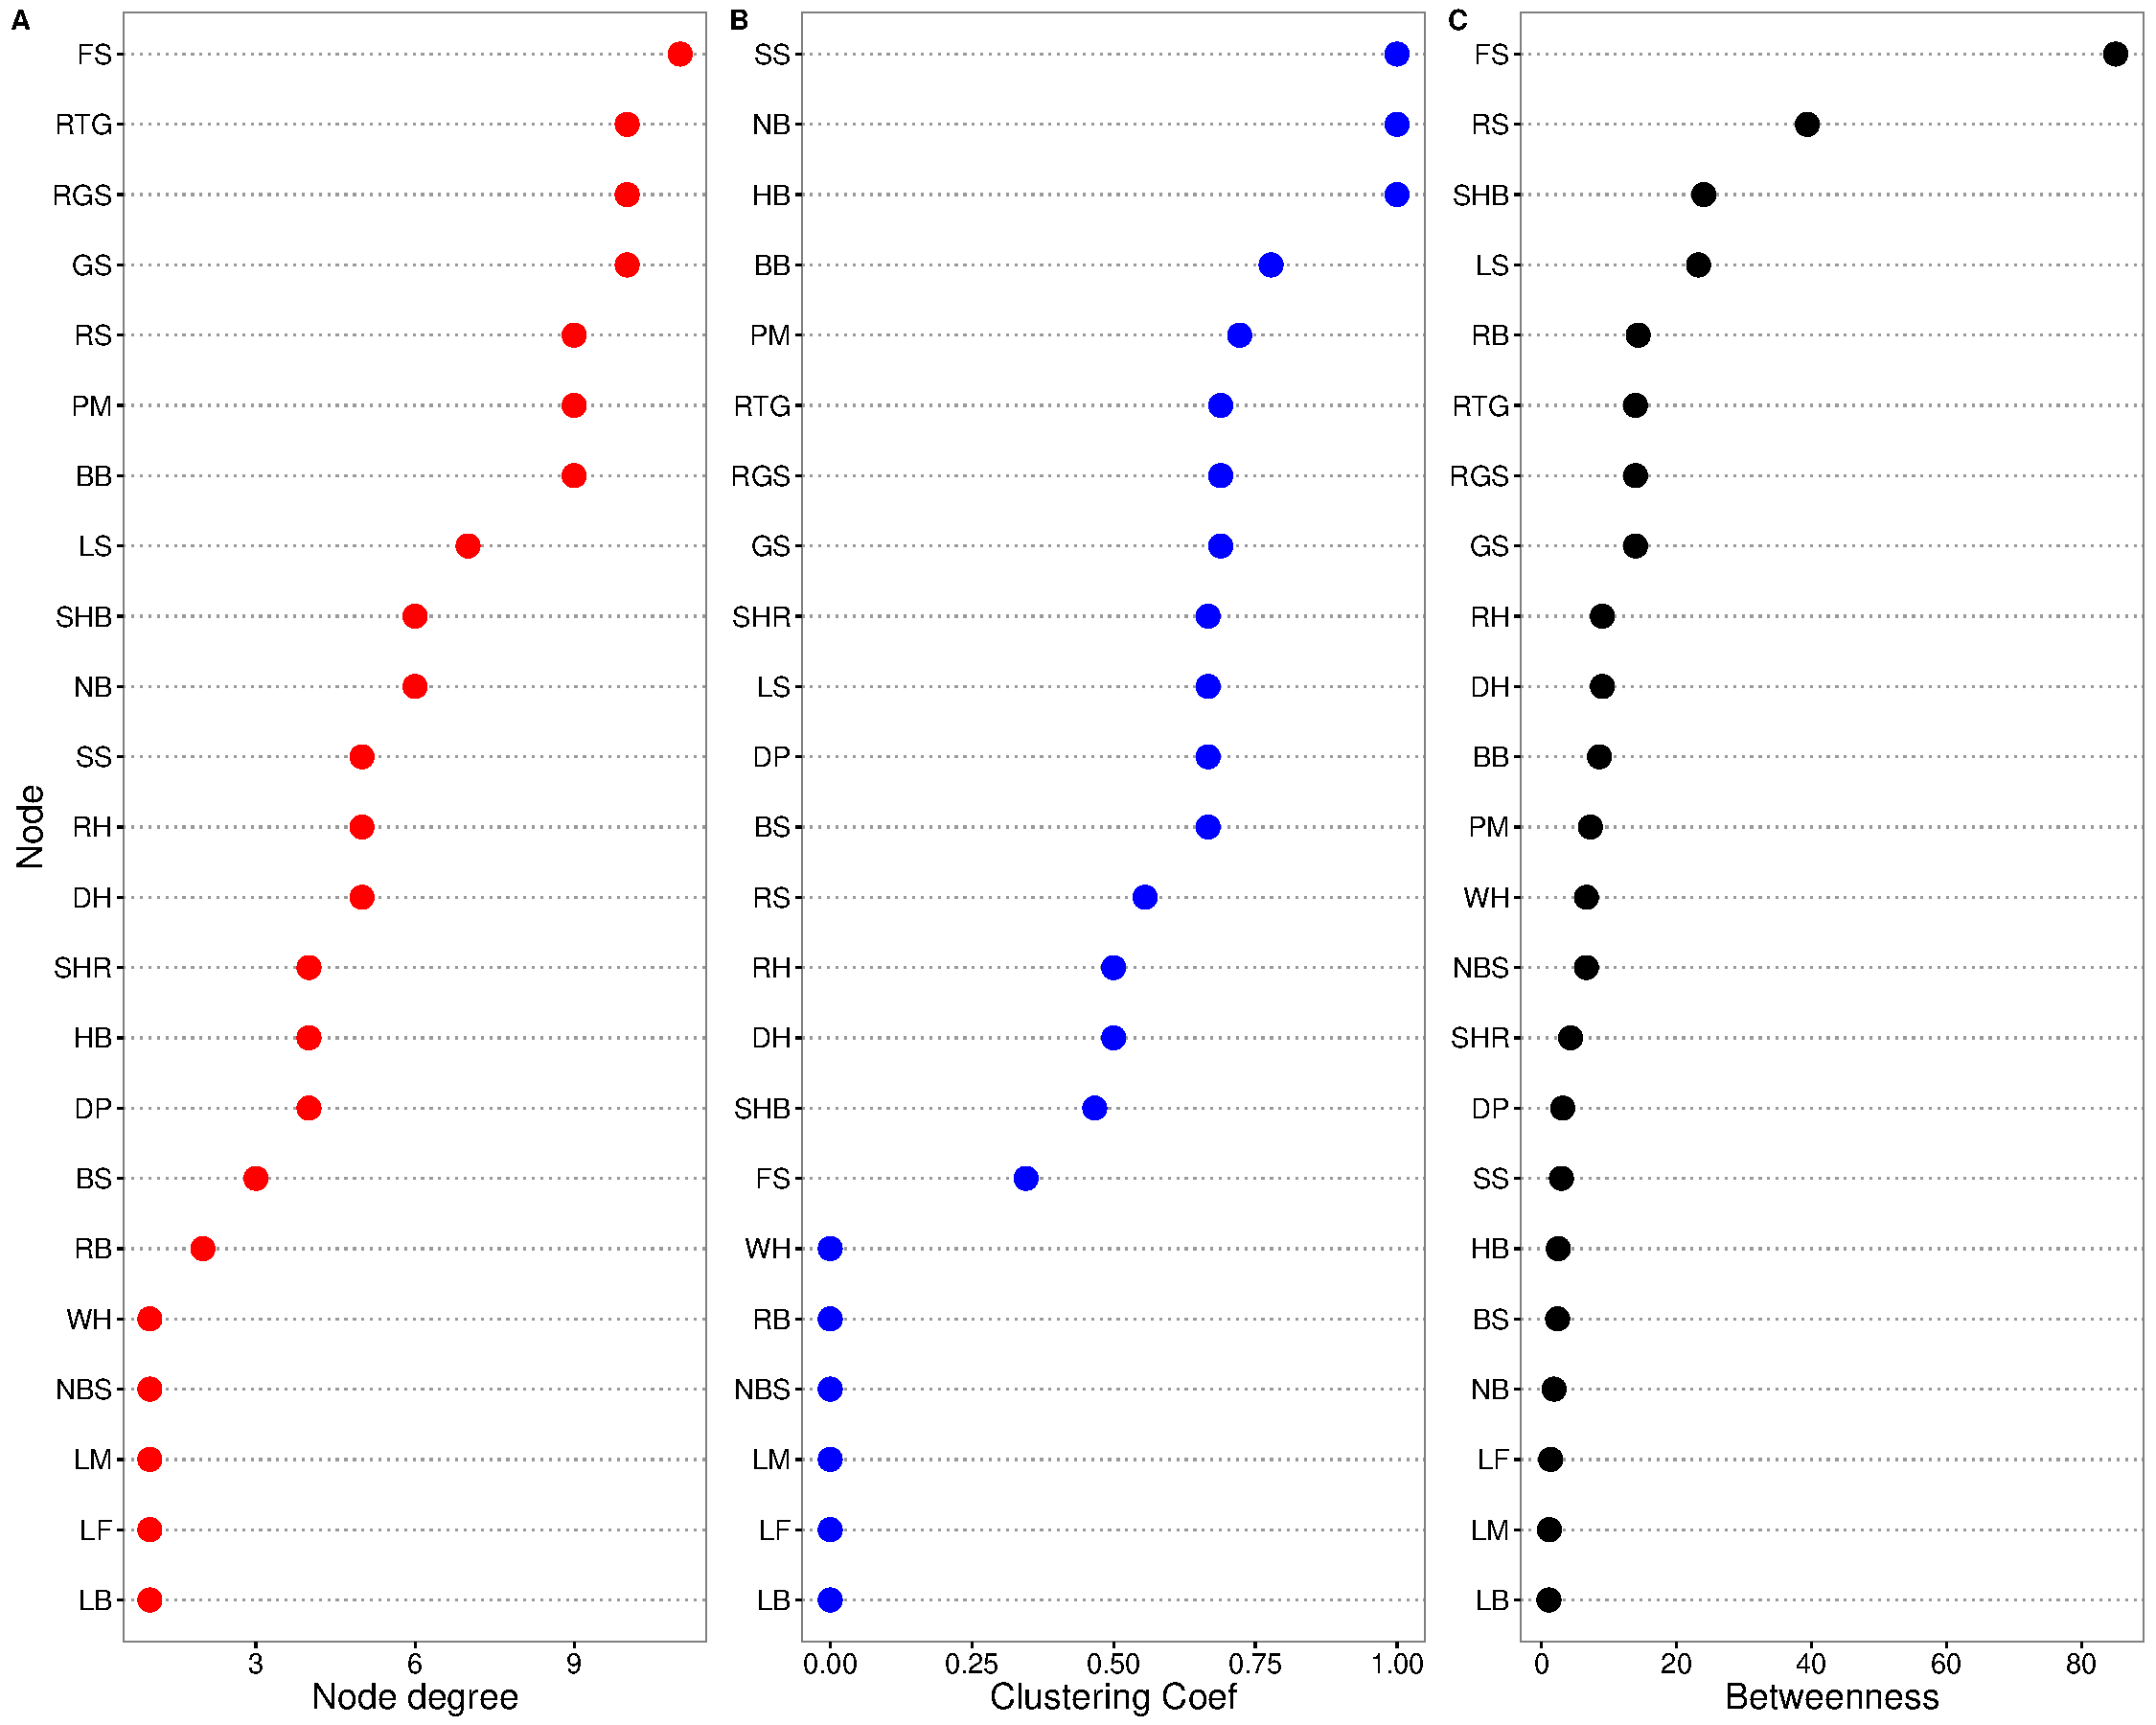
\includegraphics[width = 1\textwidth]{figures/yield_dif_nodepropWest_Java.pdf}
        \caption{Three centrality measures of the nodes in co-occurrence network of rice injuries in dry season at Central Plain. A: node degree, B:clustering coefficient, and C:Betweenness.}
        \label{fig:nodepropdifyield_WJ}
    \end{subfigure}
    \caption{Differential network analysis of survey data in different yield levels at West Java, Indonesia}
    \label{fig:yielddif_WJ}
\end{figure}


% ===
\begin{figure}[h]
    \centering
        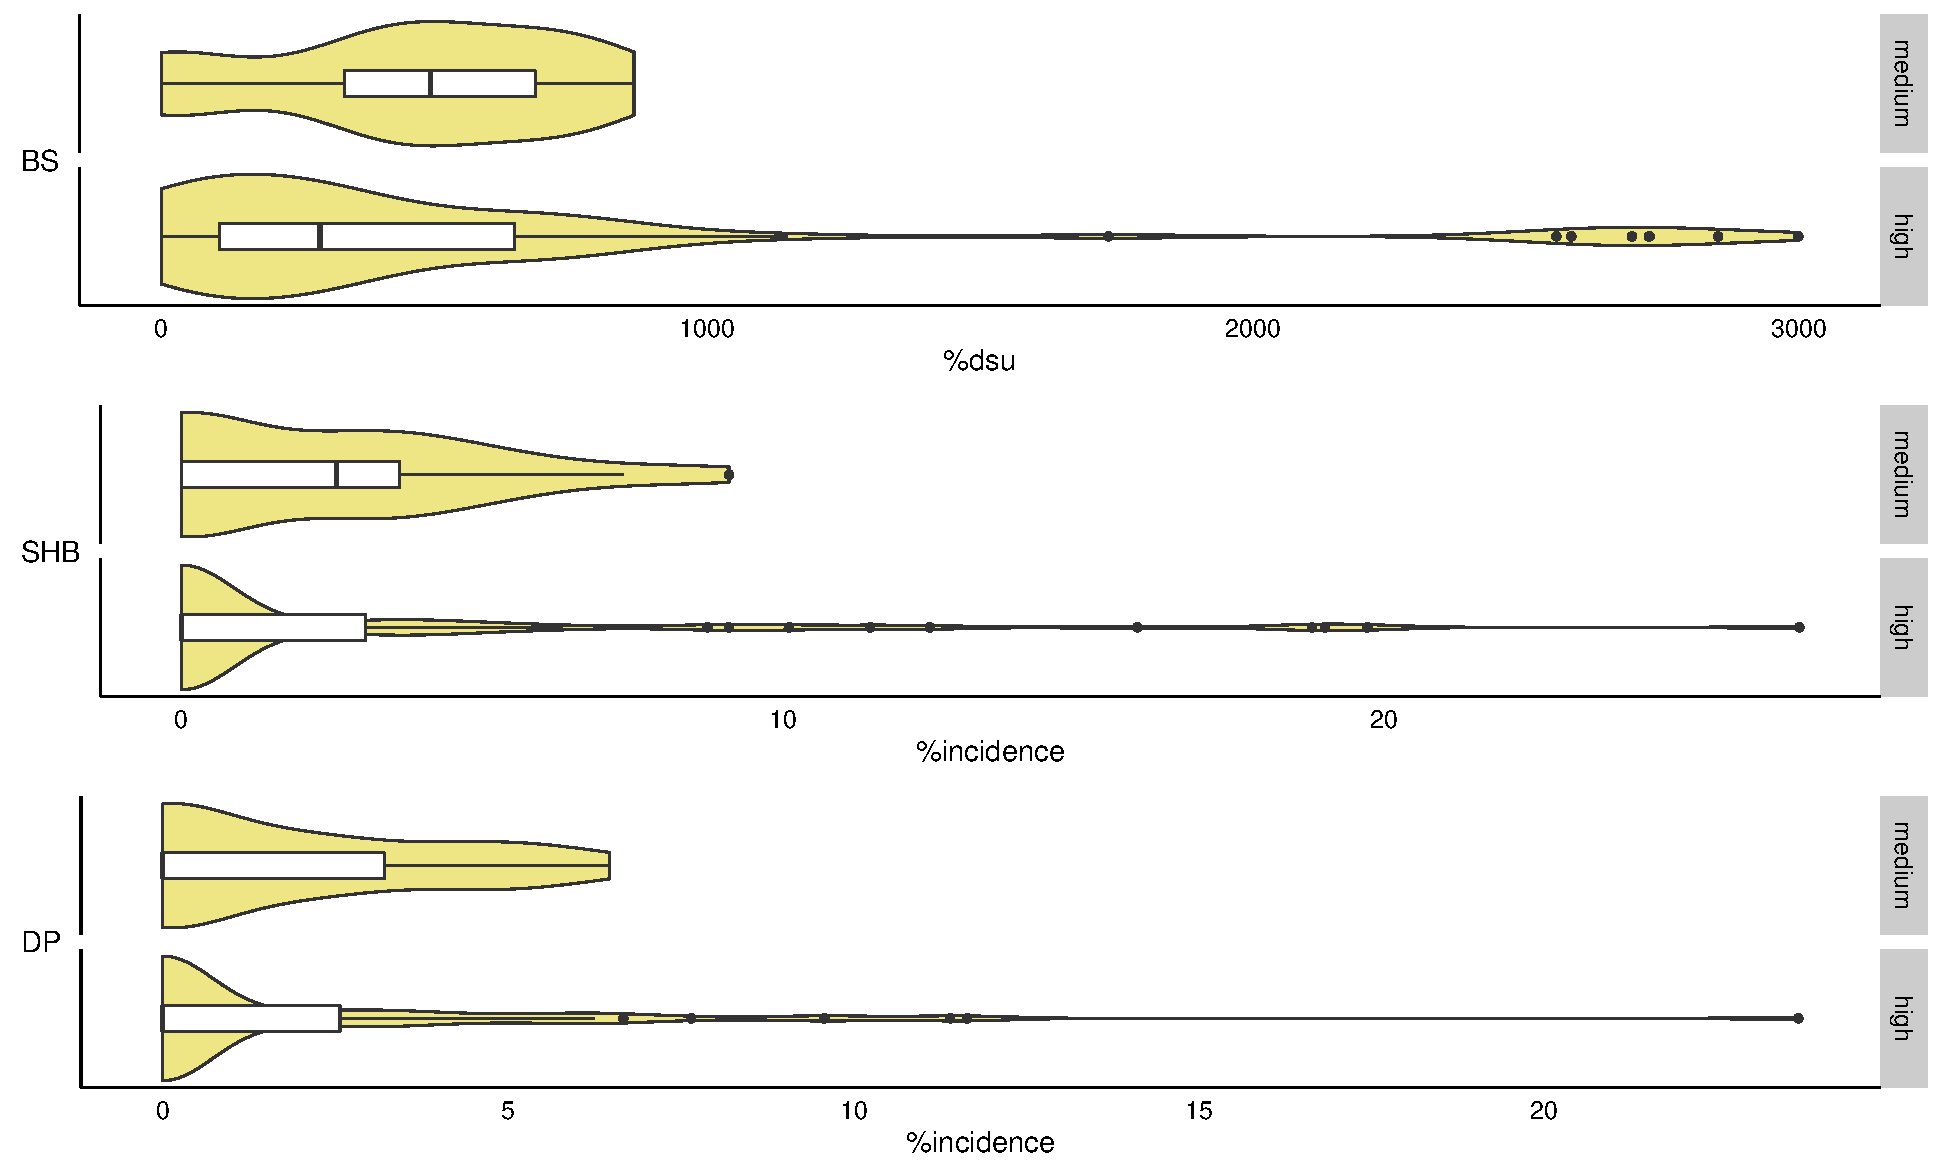
\includegraphics[width = 1\textwidth]{figures/CP_yield_box.pdf}
        \caption{.}
        \label{fig:yield.box_CP}
\end{figure}


\begin{figure}
        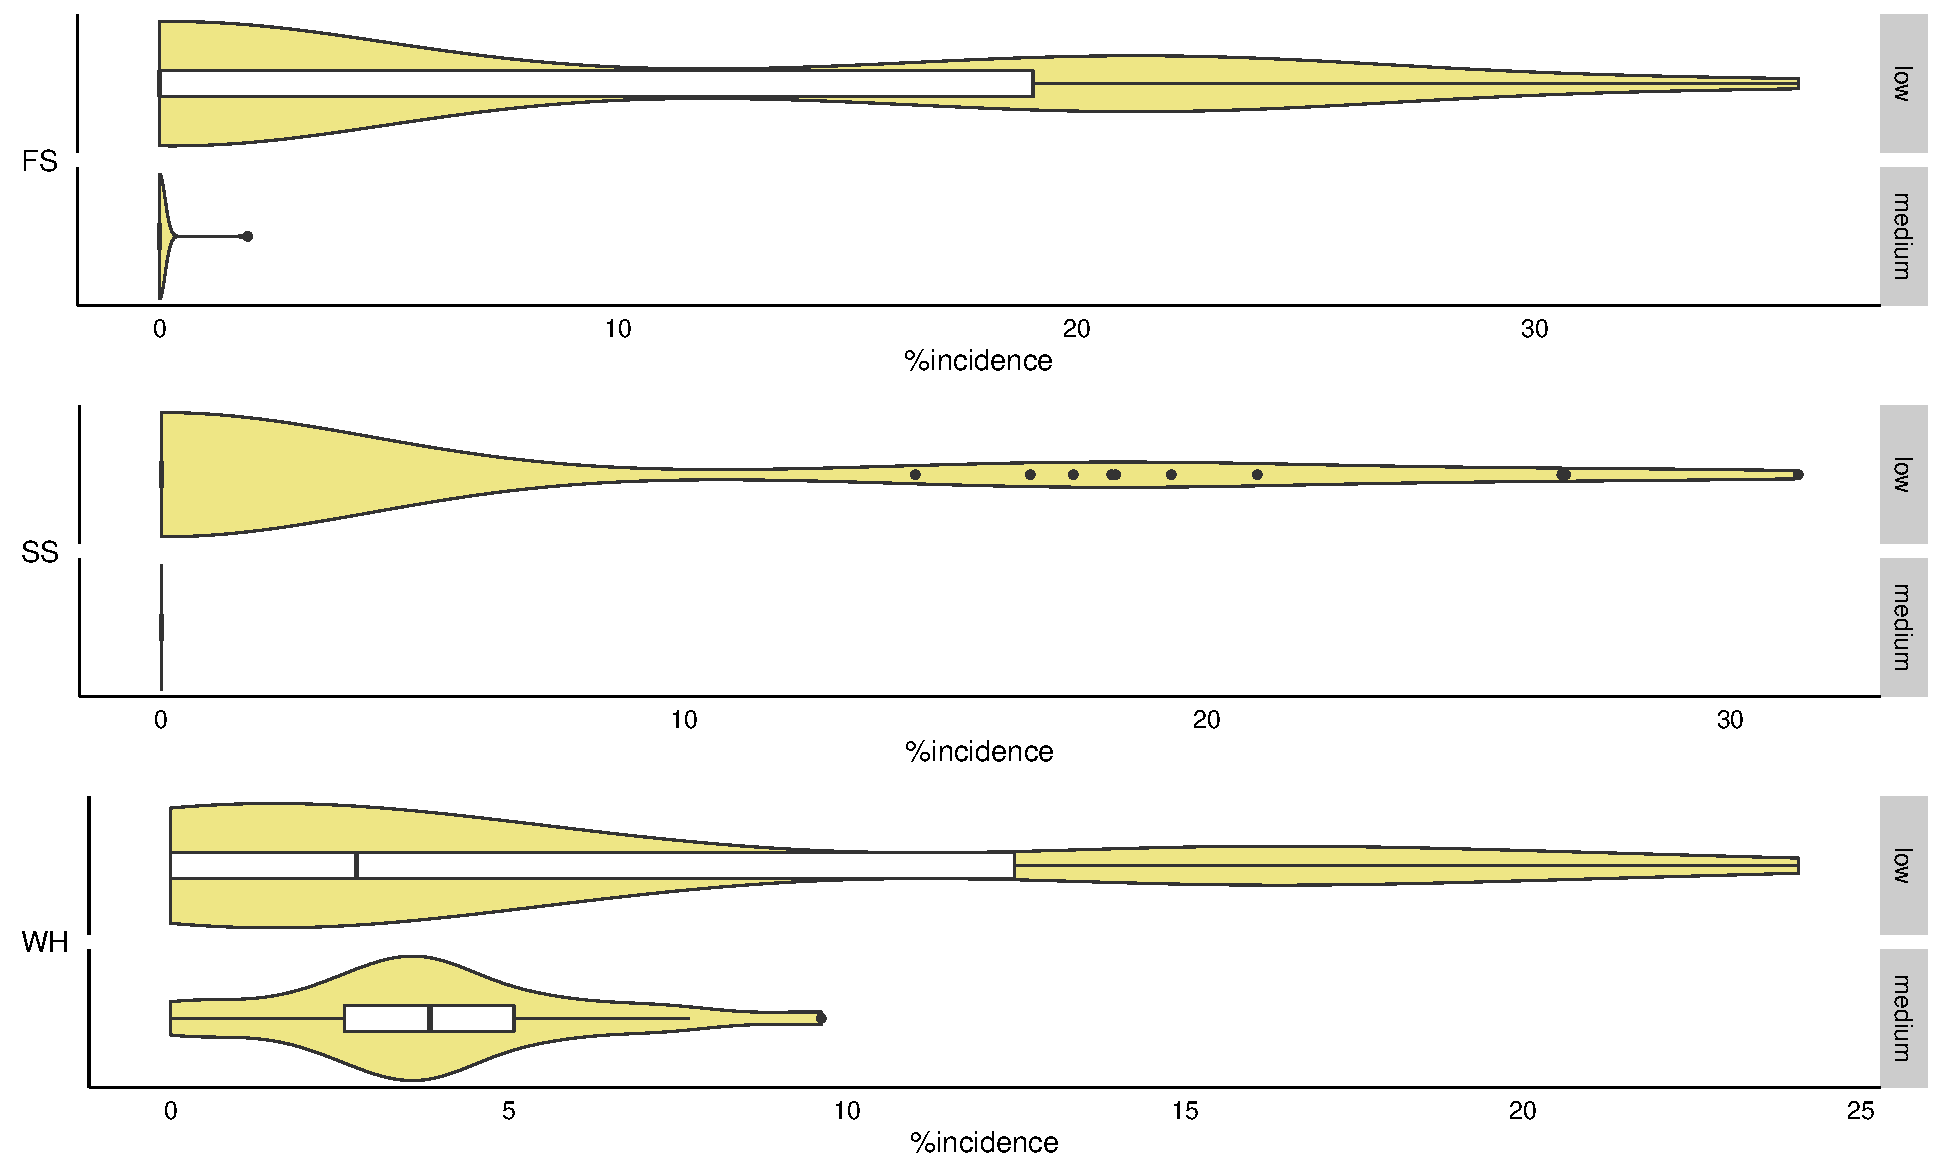
\includegraphics[width = 1\textwidth]{figures/OD_yield_box.pdf}
        \caption{.}
\label{fig:yield.box_OD}
\end{figure}

\begin{figure}
    \centering
        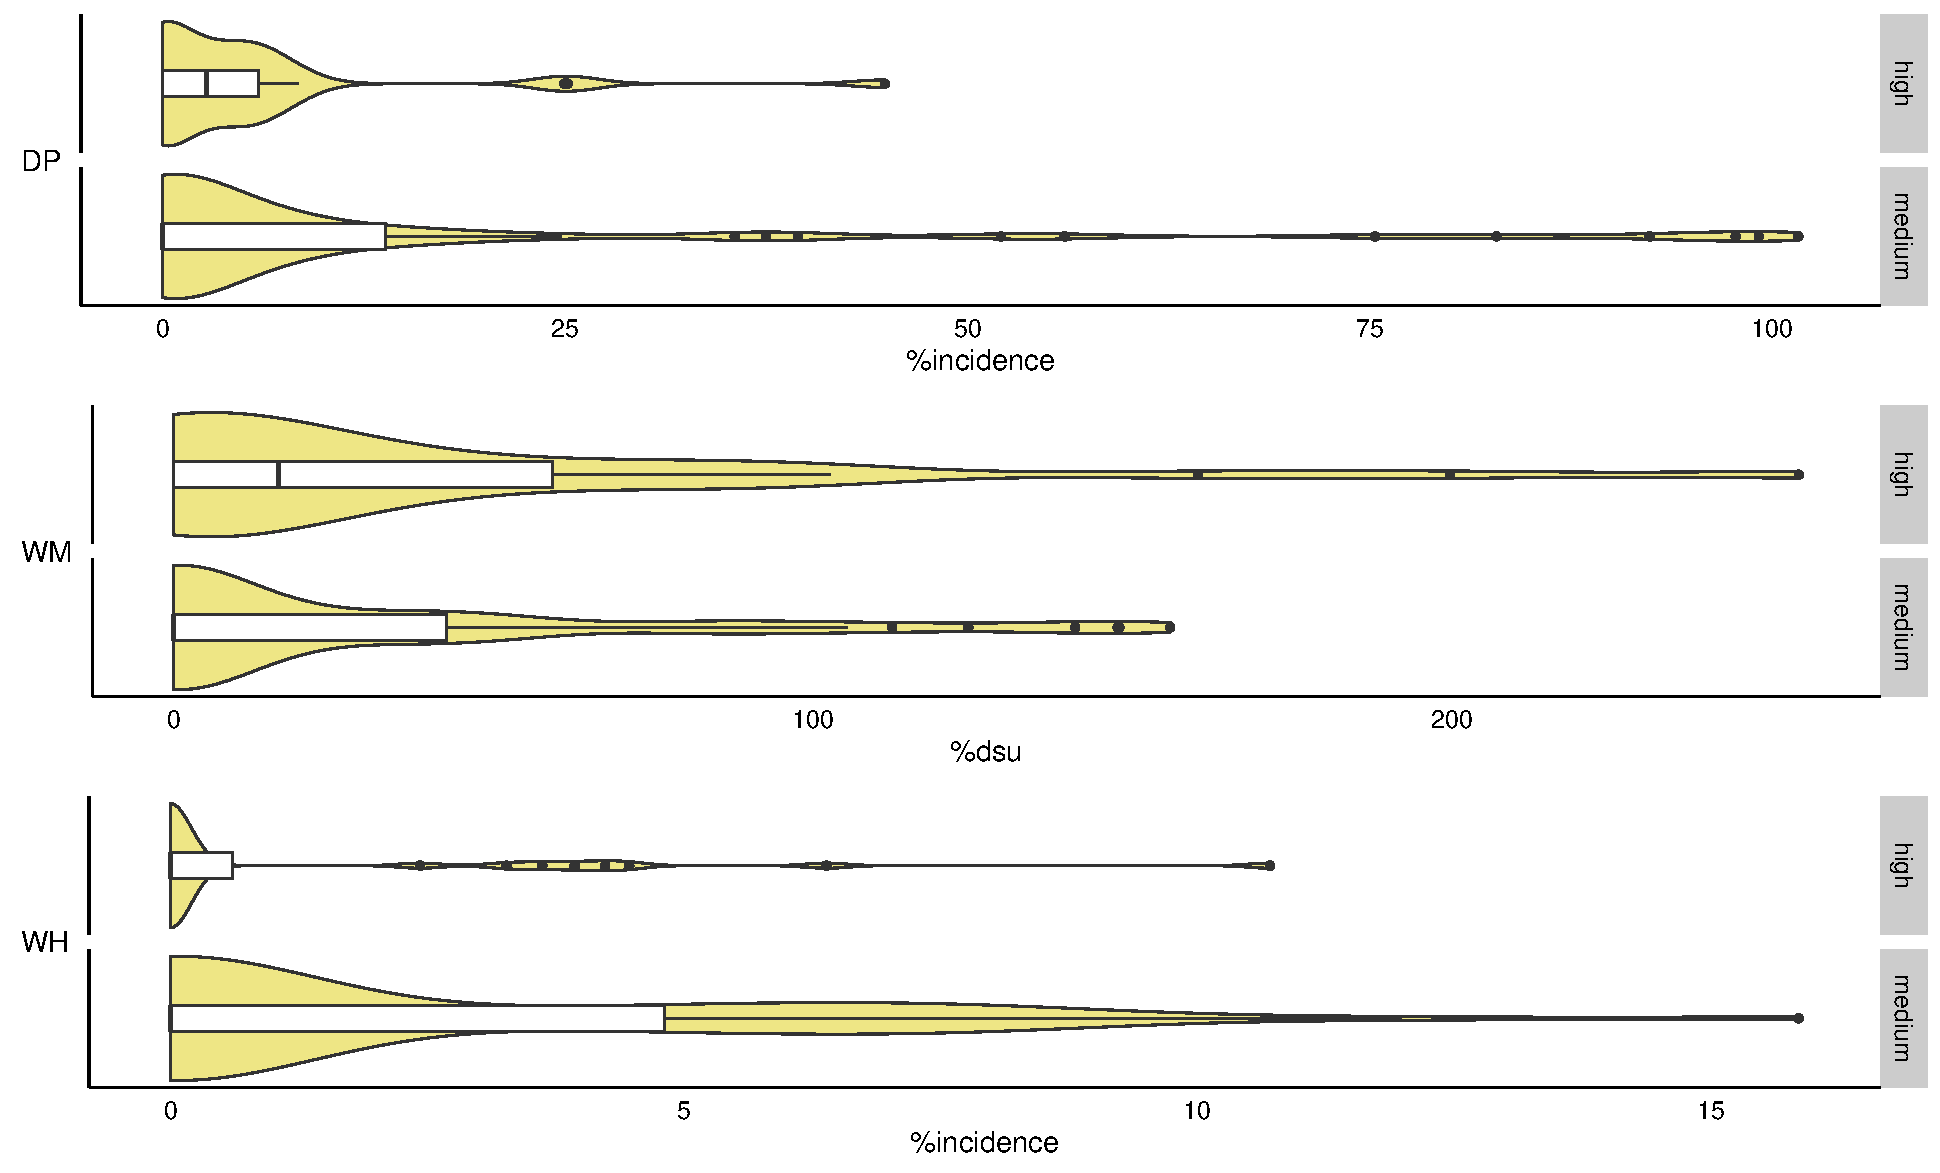
\includegraphics[width = 1\textwidth]{figures/RR_yield_box.pdf}
        \caption{.}
        \label{fig:yield.box_RR}
\end{figure}


\begin{figure}
        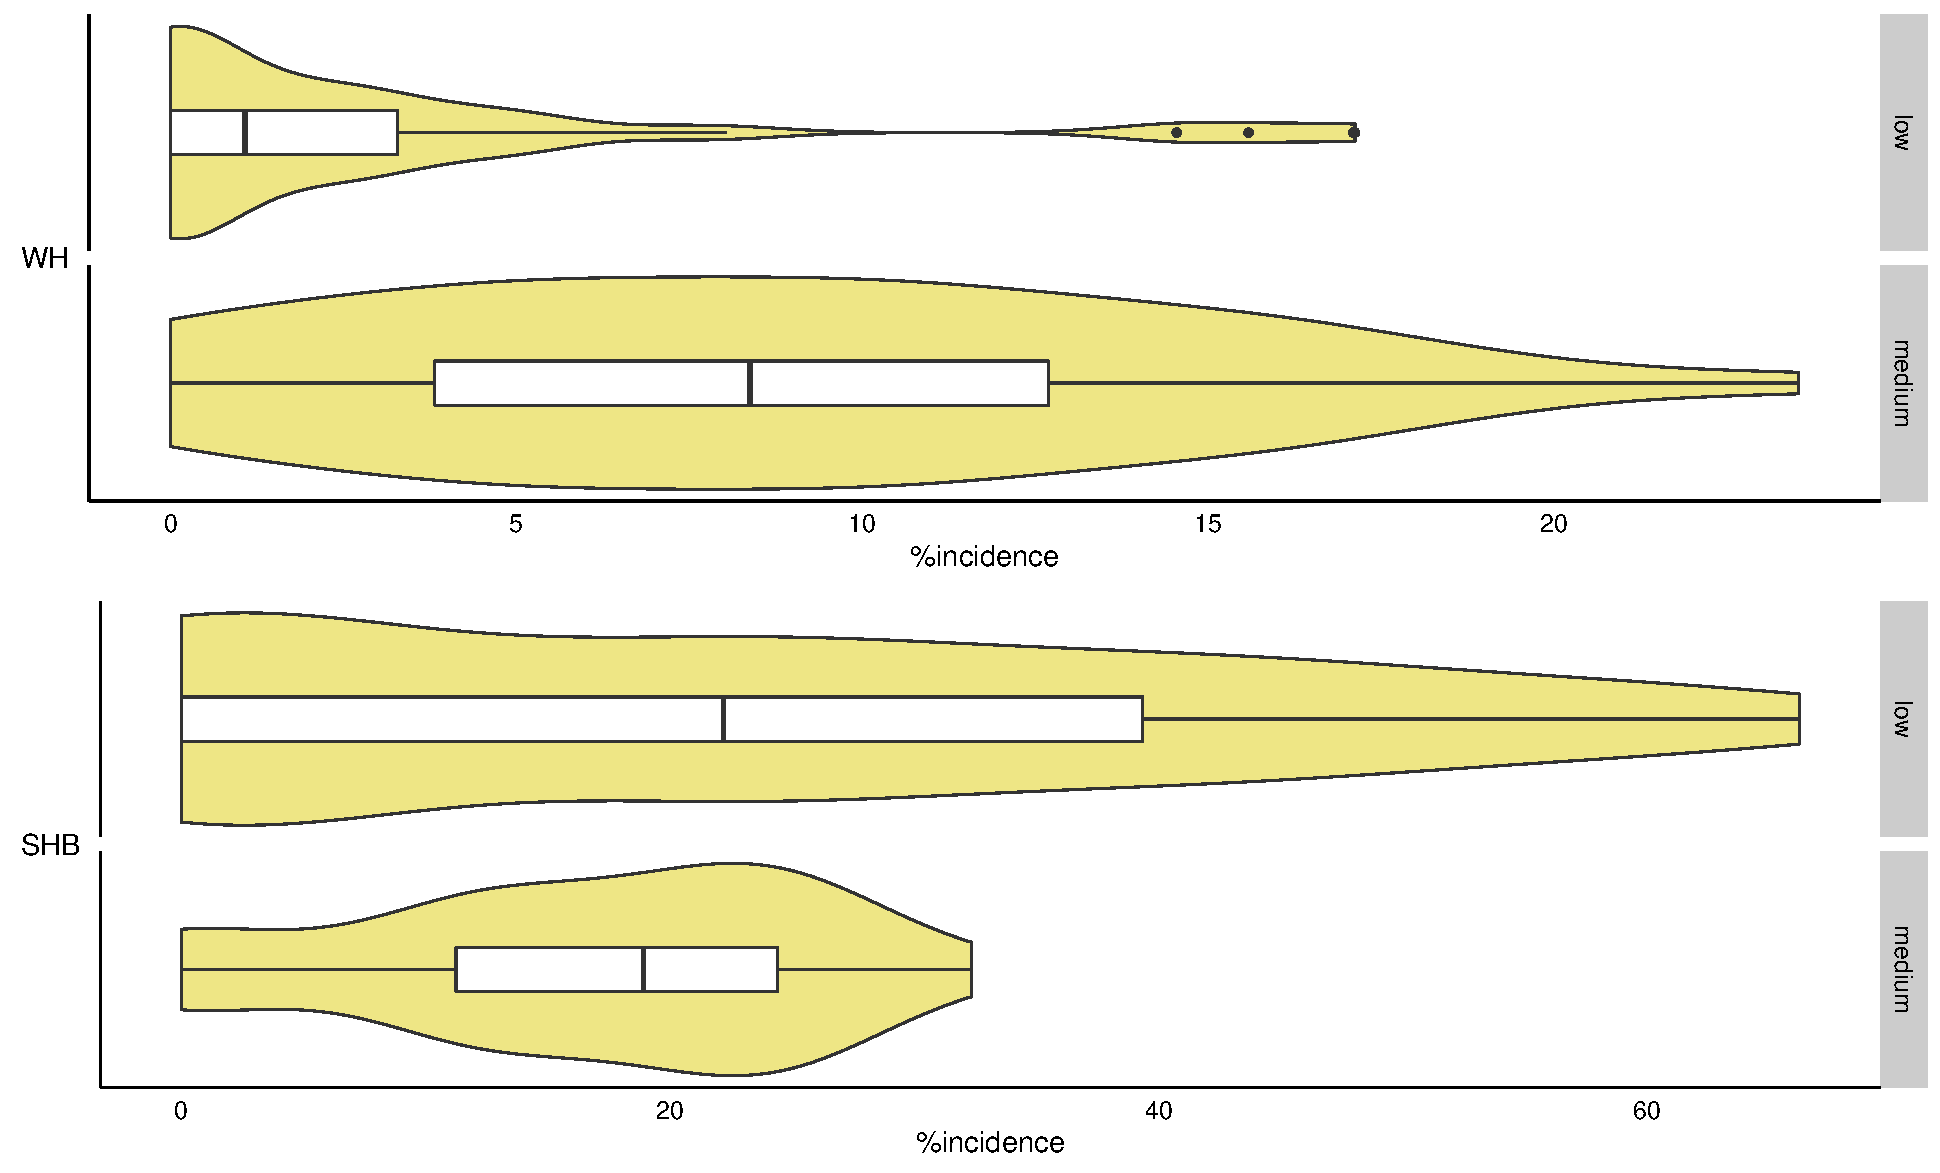
\includegraphics[width = 1\textwidth]{figures/TM_yield_box.pdf}
        \caption{.}
\label{fig:yield.box_TM}
\end{figure}

\begin{figure}
        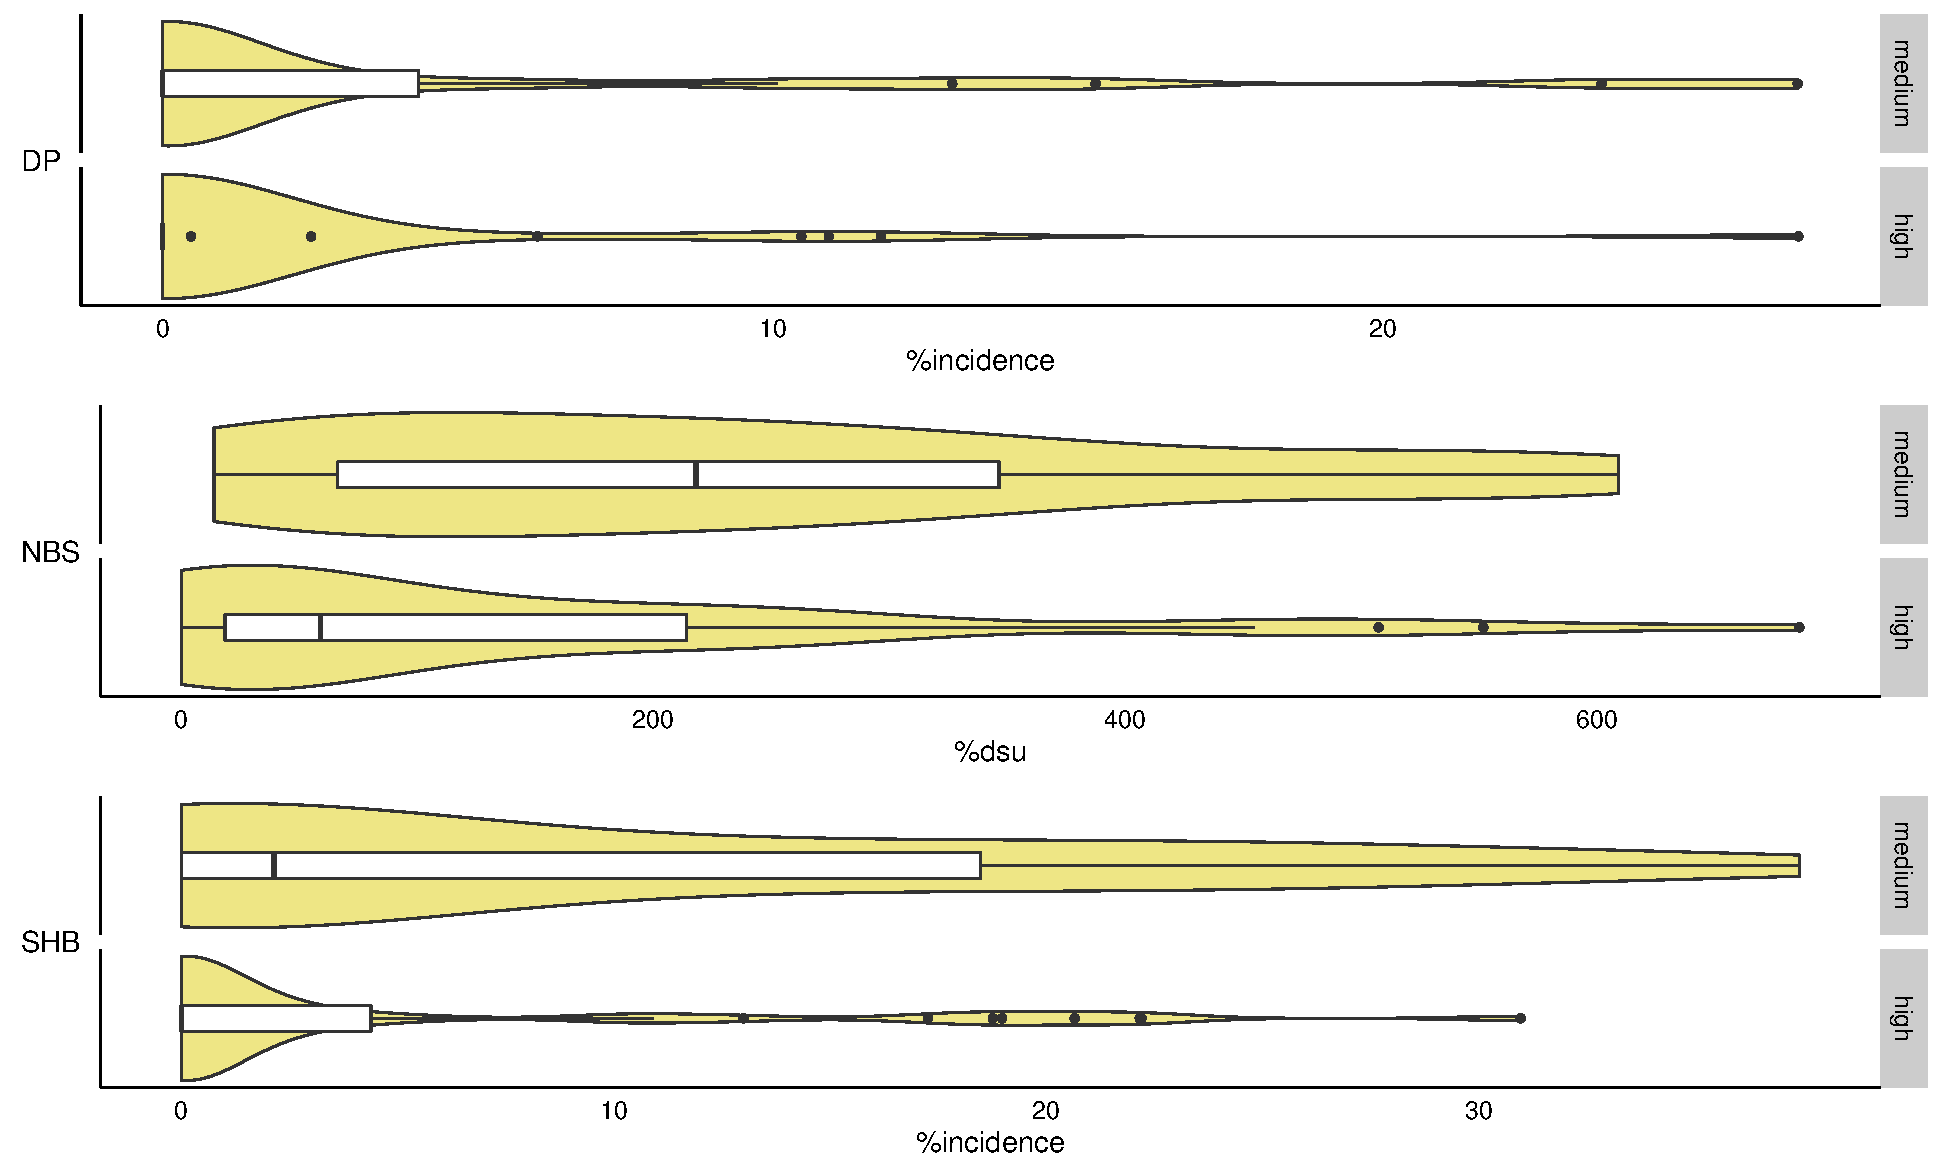
\includegraphics[width = 1\textwidth]{figures/WJ_yield_box.pdf}
        \caption{.}
\label{fig:yield.box_WJ}
\end{figure}


\clearpage
\subsection{Discussion}
When sets of changed correlations have been identified,
the next step is to establish the causal influences in the
regulatory systems (i.e. to put directions on the edges in the
undirected coexpression network) and, more importantly,
to identify which causal influences have disappeared in the
disease network with respect to the healthy network. Such
disappeared regulatory mechanisms resulted in the
observed changes in correlations and potentially could
underlie the associated disease phenotype. Although it is
not trivial to identify the causal system from the correlation
patterns, the changes in correlation hint at the
interesting regions of the network involved in disease
which could form the basis for further detailed analysis.
Systematic perturbations (e.g. experimental gene knockouts)
are needed to establish the edges’ direction. Particular
promise comes from so-called systems genetics
experiments in which genotyping and gene expression data
(and possibly metabolomics and proteomic

%Systems biology methods like this are in high demand as the differences between many conditions, be they neurodegenerative diseases, brain diseases, different kinds of cancers, different degrees of disease severity, and so forth, are very subtle and cannot be easily highlighted using the usual off-the-shelf clustering or biological pathways identification algorithms. Many studies investigate only the genes that are unique to a condition, in order to analyze how different the conditions are. However, we hypothesize that even the genes that are common between conditions (conditions can be physiological, treatment, or time) can contribute to the differences between conditions either by invoking different biological pathways or by invoking the same biological pathways to varying degrees. Our differential network analysis method is applicable to other studies where a sequence of activities or processes is being determined. For instance, in our time-dependent analysis of low dose ionizing radiation study we were able to show the active biological processes at 3, 8, and 24 hours [12]. Our approach can aid in identifying the few genes that may be the key players in the specific condition and, therefore, potential biomarkers or therapeutic targets for that condition.

 
%----------------------------------------------------------------------
% END MATERIAL
%----------------------------------------------------------------------

% B I B L I O G R A P H Y
% -----------------------
\bibliographystyle{apalike2}
\cleardoublepage
\begin{singlespace}
\renewcommand{\bibname}{LITERATURE CITED}
\bibliography{bibliography/biblio}
\end{singlespace}
\end{document}